% Auto-generated by scripts/generate_heatmap_figures_tex.py
% One figure per (token, position); 3 rows x 5 cols inside each figure.

\begin{figure}[H]
\centering
\setlength{\tabcolsep}{2pt}
\renewcommand{\arraystretch}{0.5}
\begin{tabular}{r ccccc}
& \textbf{rep=1} & \textbf{rep=2} & \textbf{rep=3} & \textbf{rep=4} & \textbf{rep=5} \\[2pt]
\rotatebox{90}{\textbf{forward}} & 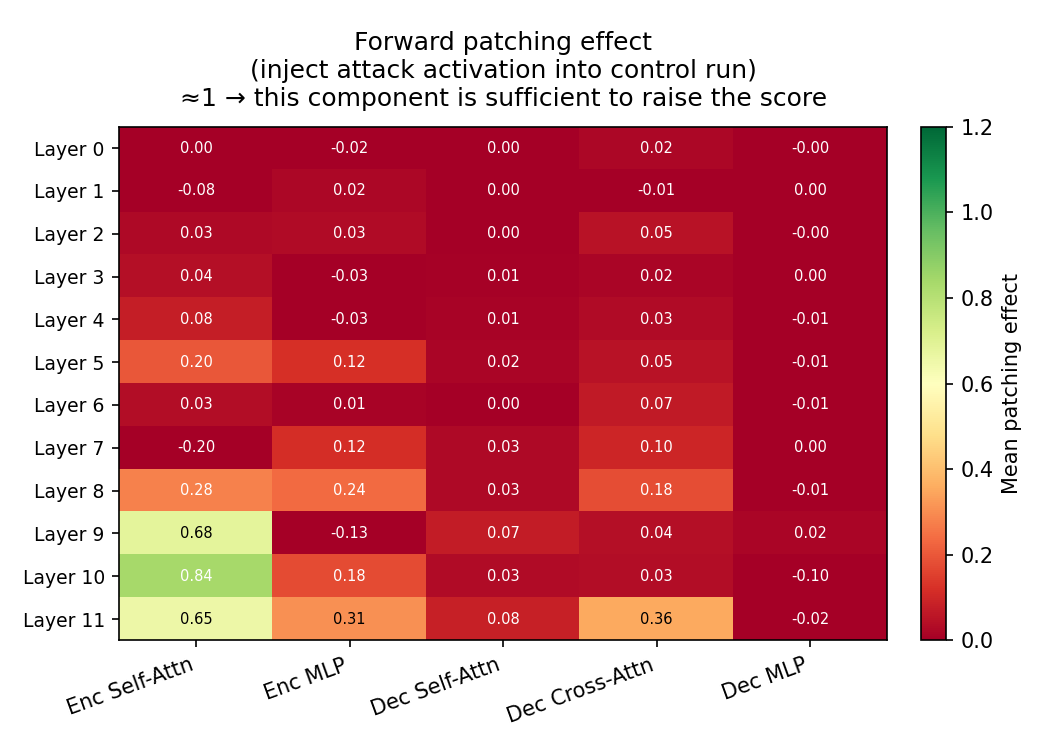
\includegraphics[width=0.17\textwidth]{outputs/attacks/bar_end_1/plots/forward_layer_component_heatmap.png} & 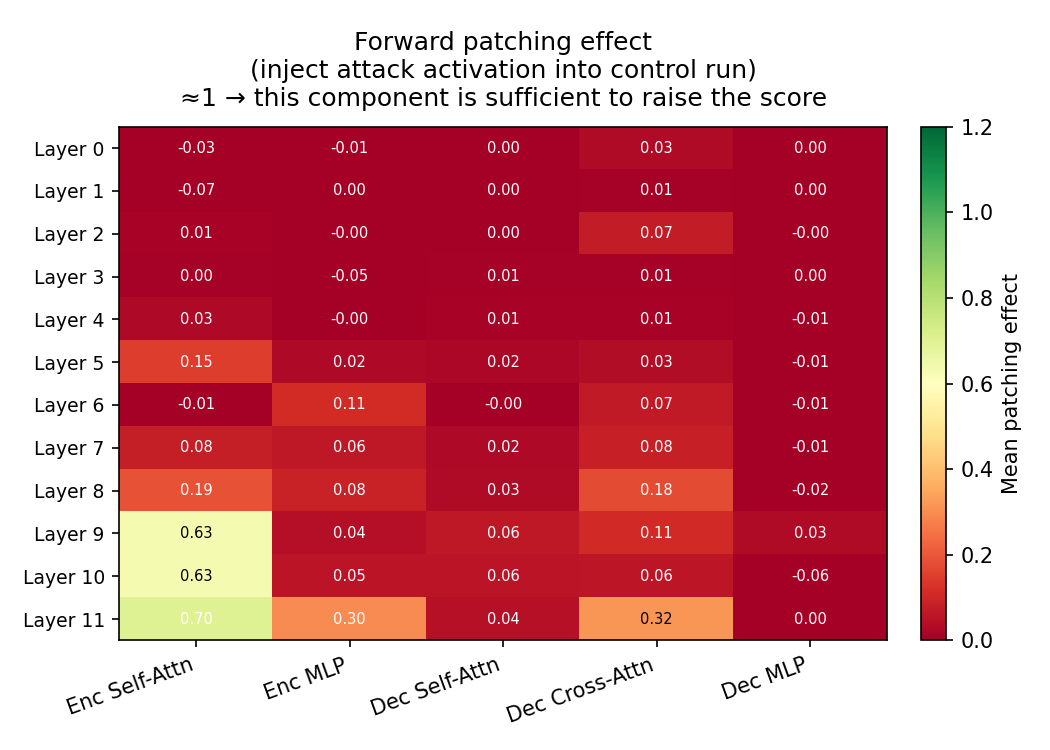
\includegraphics[width=0.17\textwidth]{outputs/attacks/bar_end_2/plots/forward_layer_component_heatmap.png} & 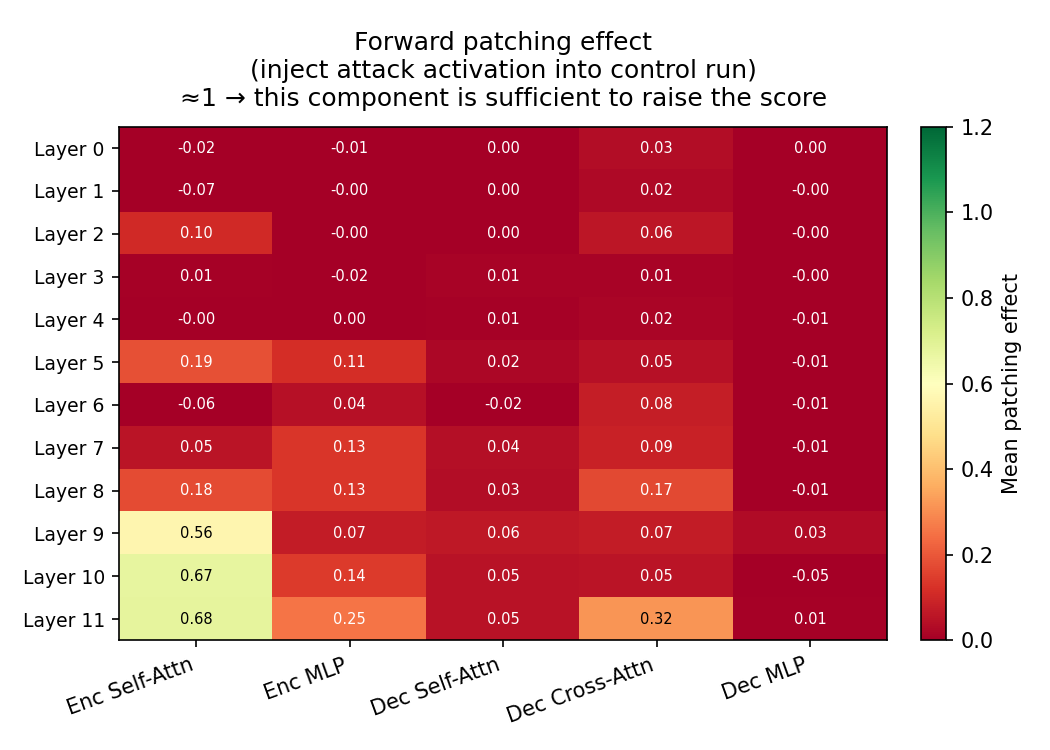
\includegraphics[width=0.17\textwidth]{outputs/attacks/bar_end_3/plots/forward_layer_component_heatmap.png} & 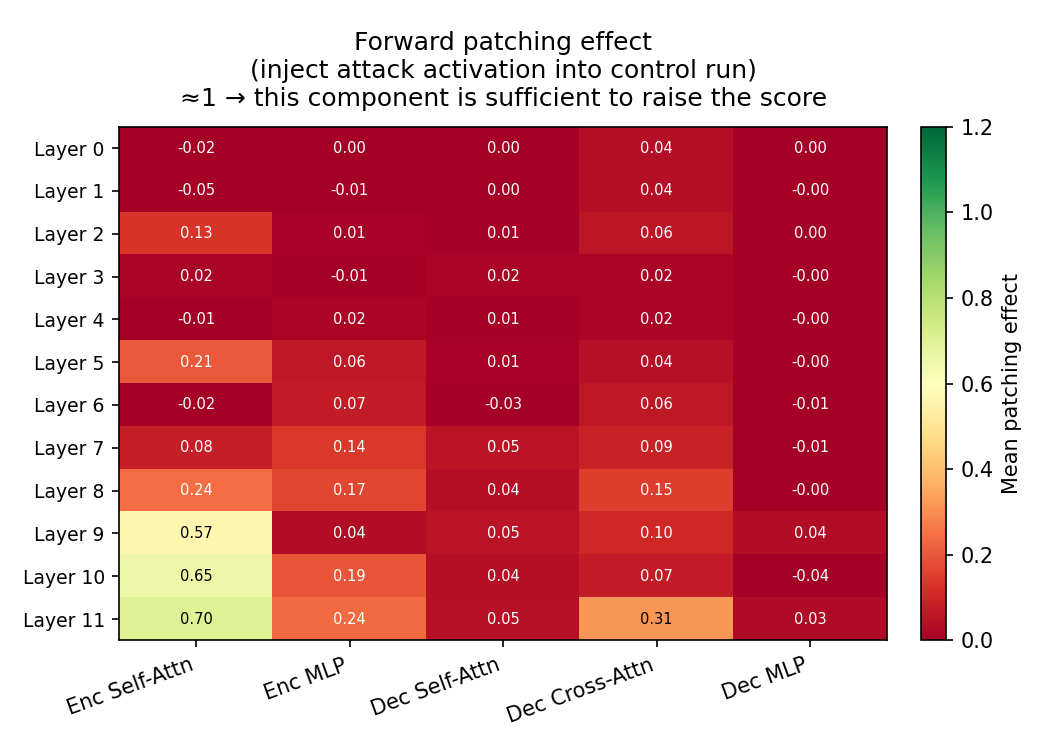
\includegraphics[width=0.17\textwidth]{outputs/attacks/bar_end_4/plots/forward_layer_component_heatmap.png} & 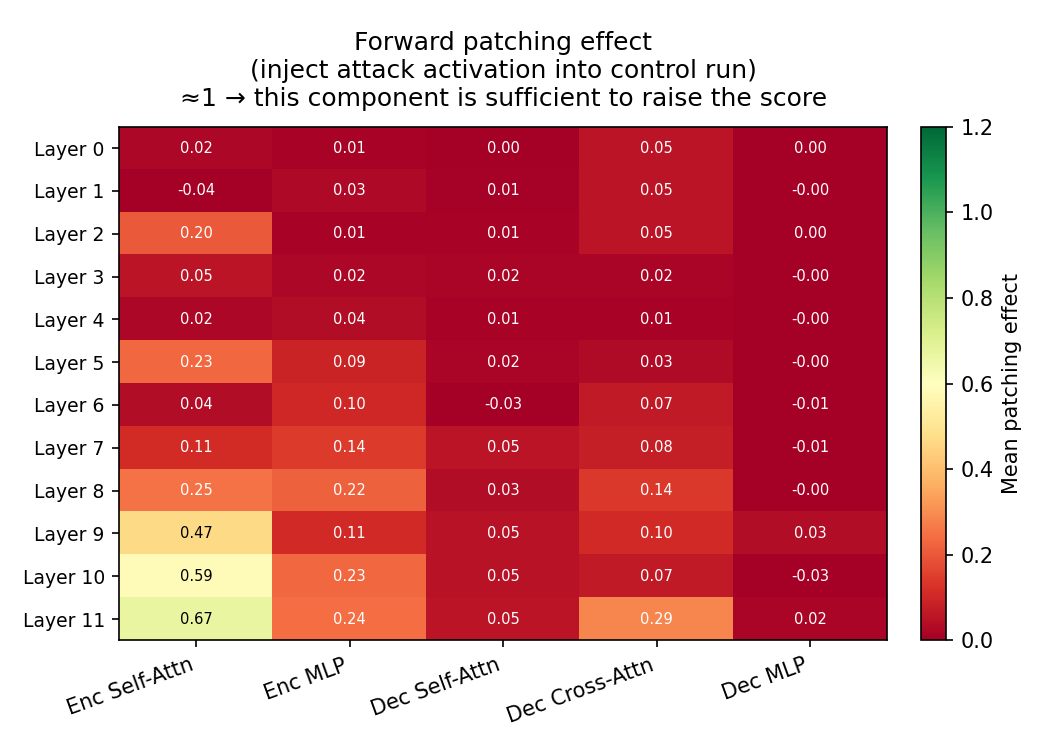
\includegraphics[width=0.17\textwidth]{outputs/attacks/bar_end_5/plots/forward_layer_component_heatmap.png} \\[4pt]
\rotatebox{90}{\textbf{reverse}} & 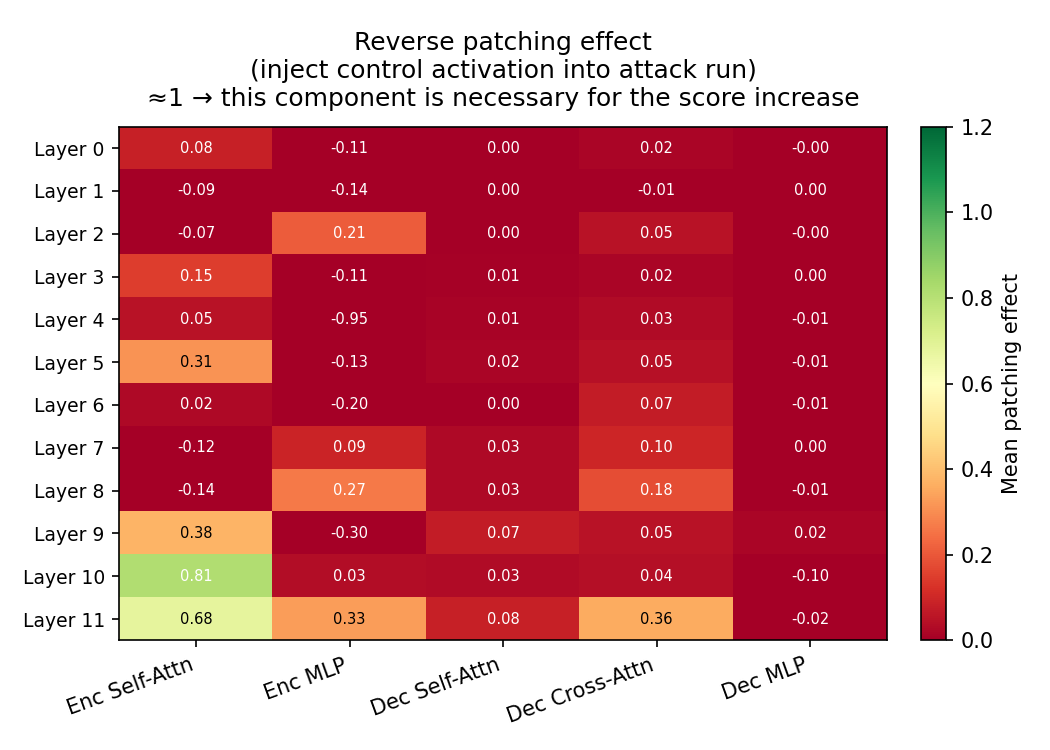
\includegraphics[width=0.17\textwidth]{outputs/attacks/bar_end_1/plots/reverse_layer_component_heatmap.png} & 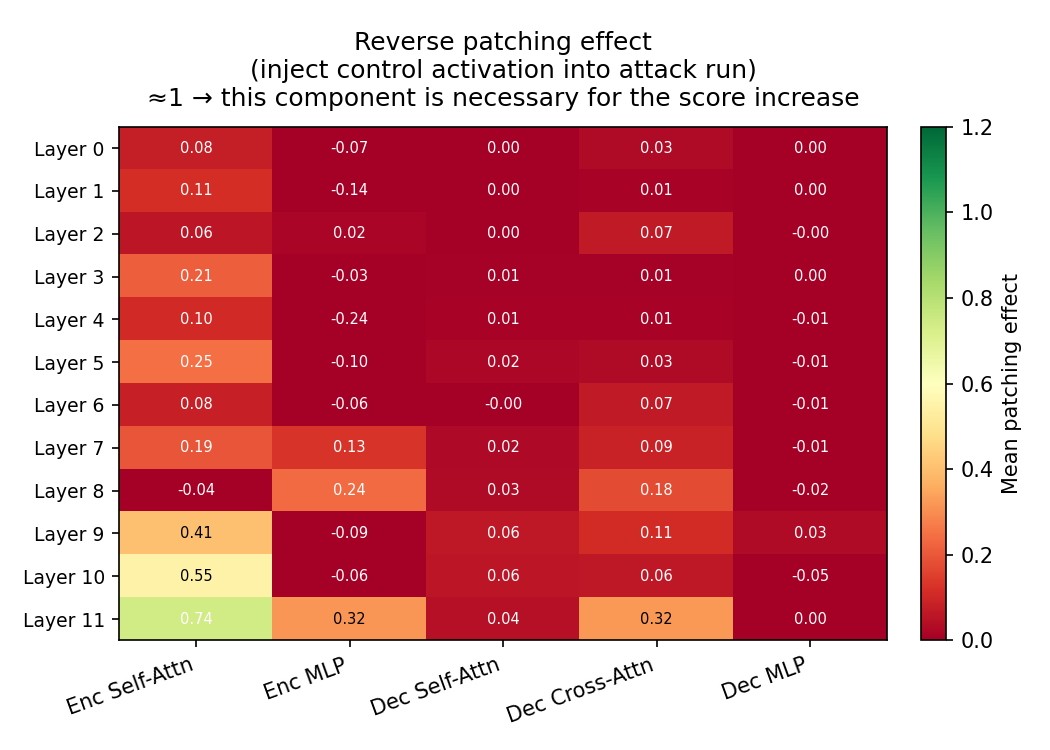
\includegraphics[width=0.17\textwidth]{outputs/attacks/bar_end_2/plots/reverse_layer_component_heatmap.png} & 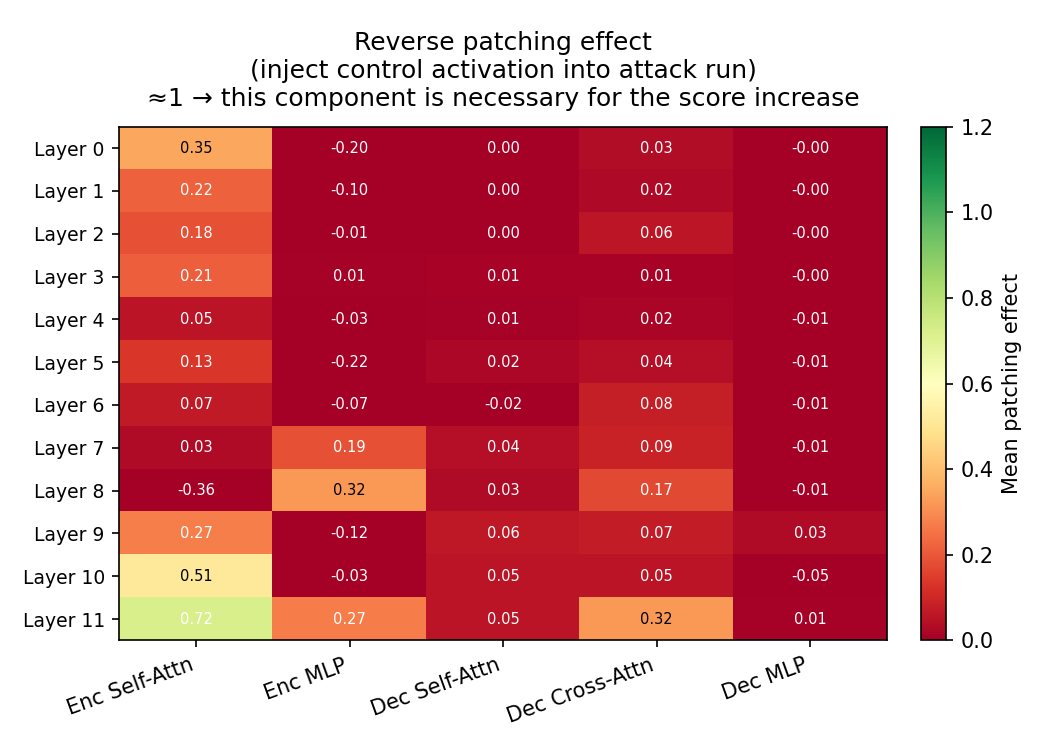
\includegraphics[width=0.17\textwidth]{outputs/attacks/bar_end_3/plots/reverse_layer_component_heatmap.png} & 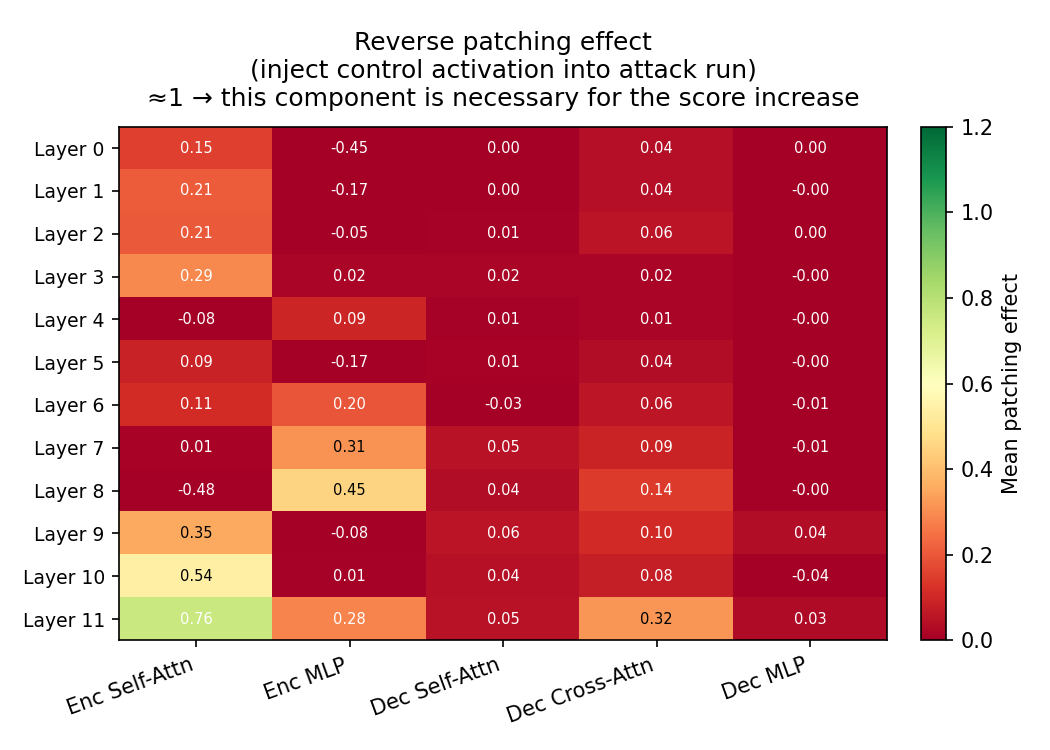
\includegraphics[width=0.17\textwidth]{outputs/attacks/bar_end_4/plots/reverse_layer_component_heatmap.png} & 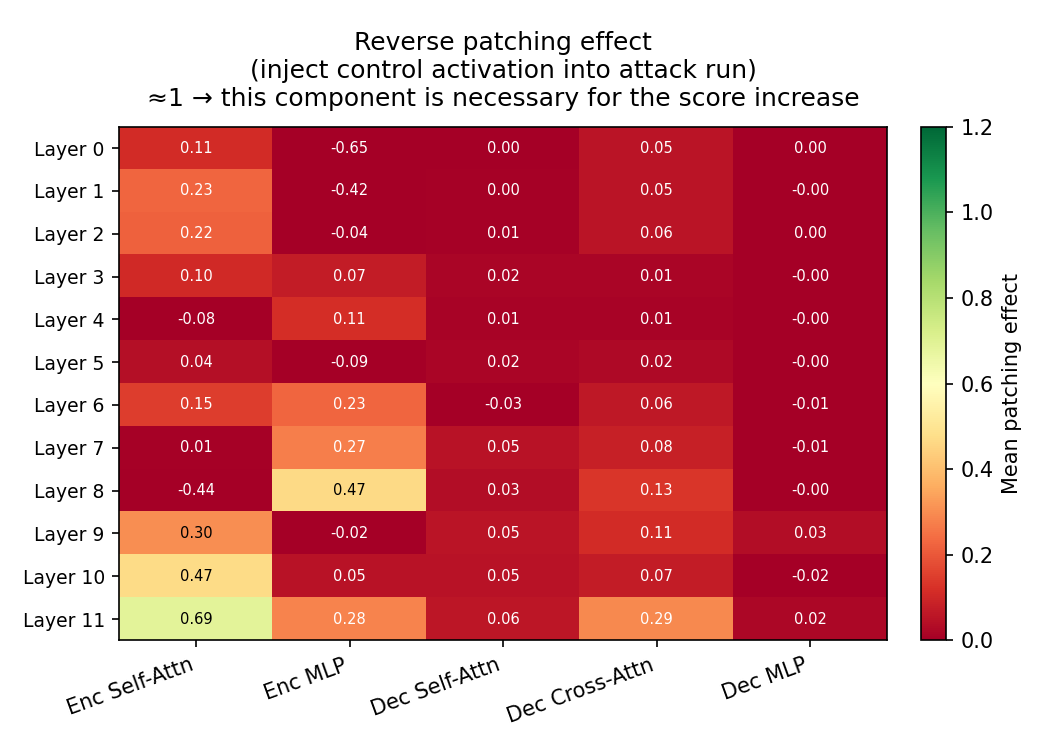
\includegraphics[width=0.17\textwidth]{outputs/attacks/bar_end_5/plots/reverse_layer_component_heatmap.png} \\[4pt]
\rotatebox{90}{\textbf{combined}} & 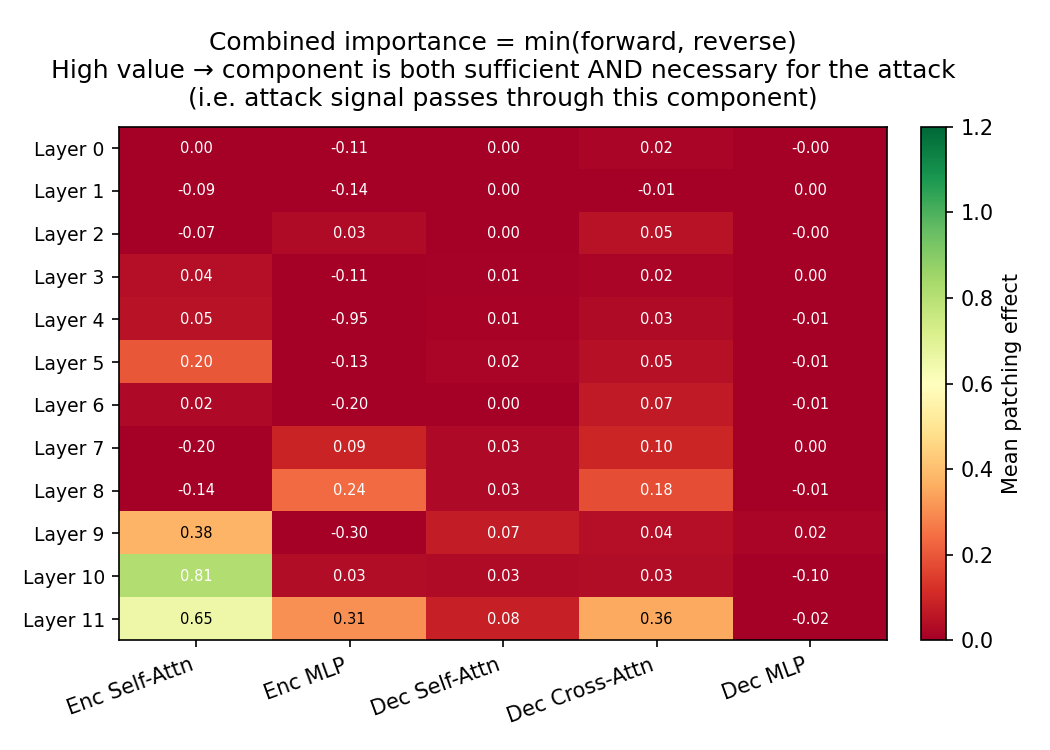
\includegraphics[width=0.17\textwidth]{outputs/attacks/bar_end_1/plots/combined_layer_component_heatmap.png} & 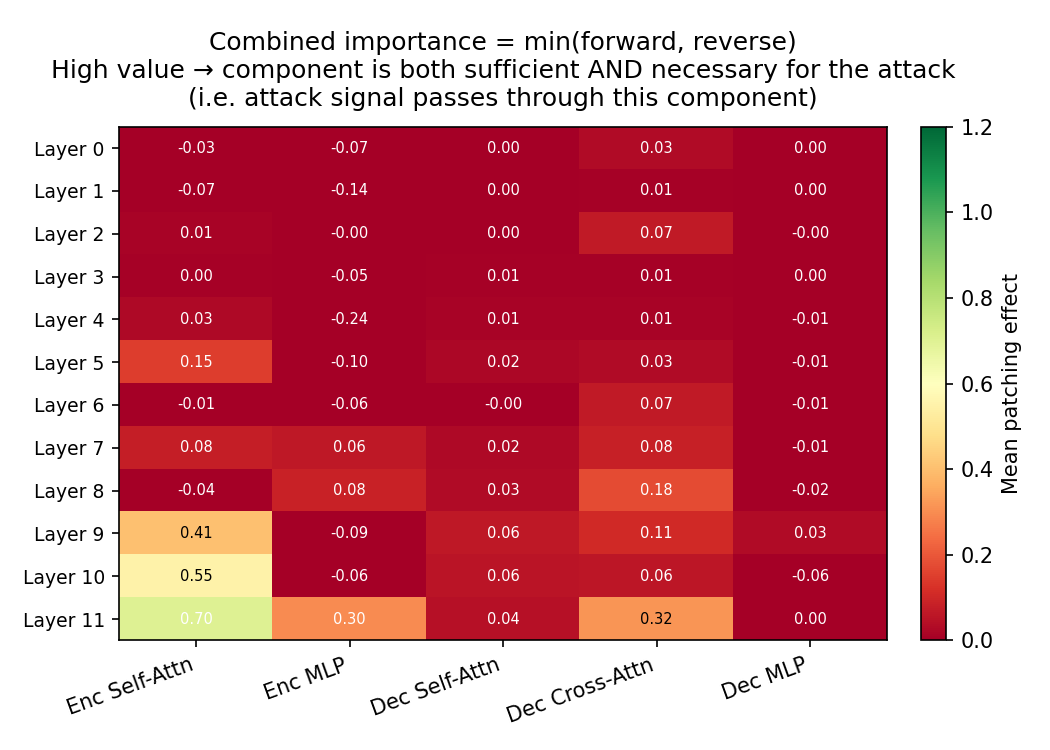
\includegraphics[width=0.17\textwidth]{outputs/attacks/bar_end_2/plots/combined_layer_component_heatmap.png} & 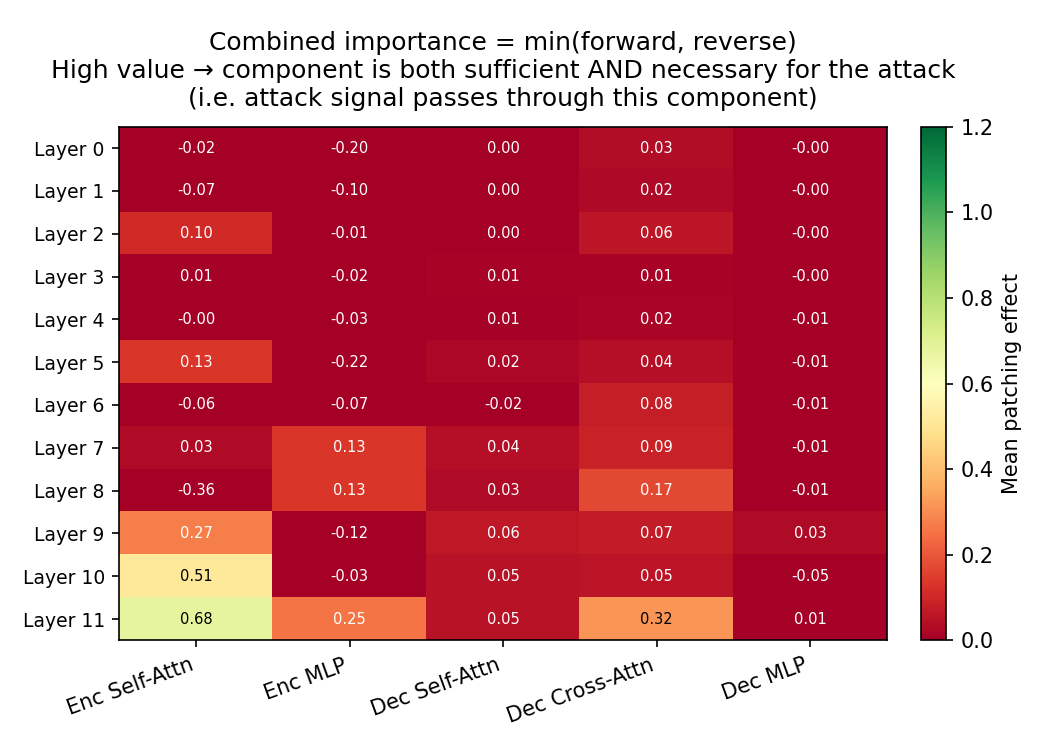
\includegraphics[width=0.17\textwidth]{outputs/attacks/bar_end_3/plots/combined_layer_component_heatmap.png} & 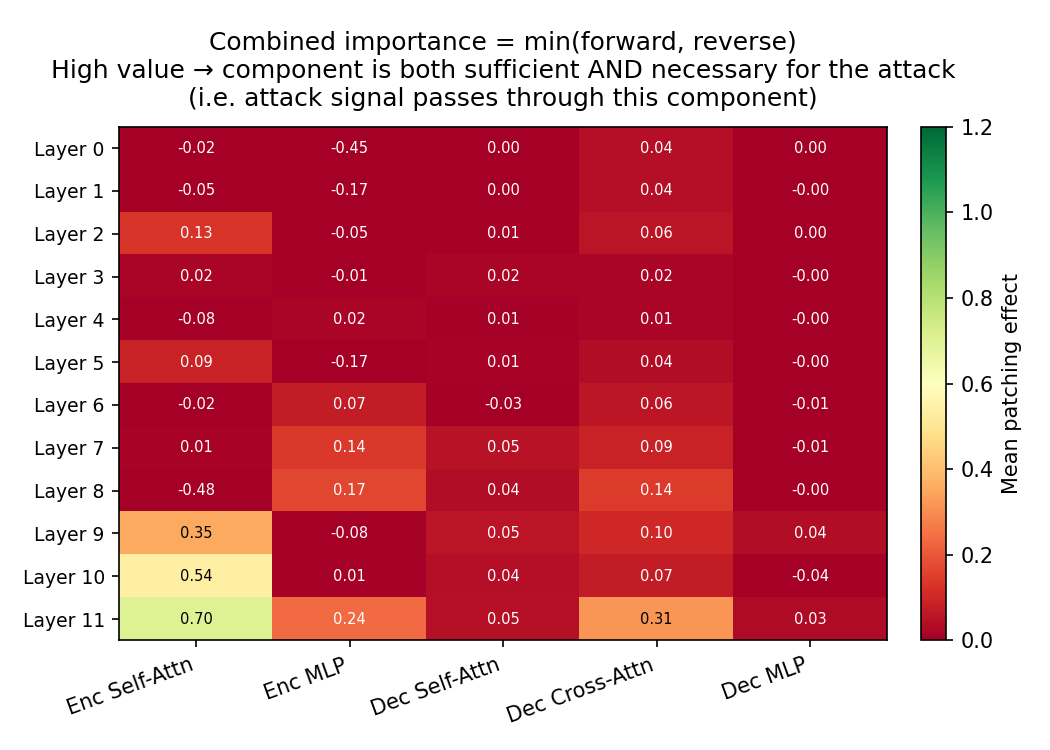
\includegraphics[width=0.17\textwidth]{outputs/attacks/bar_end_4/plots/combined_layer_component_heatmap.png} & 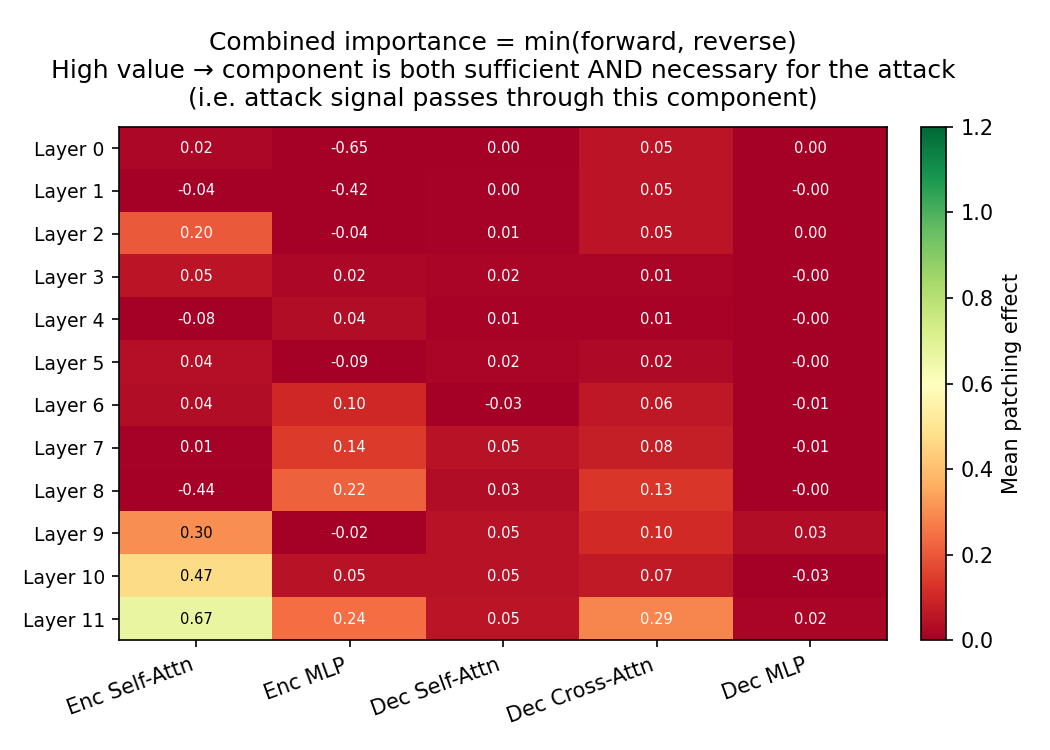
\includegraphics[width=0.17\textwidth]{outputs/attacks/bar_end_5/plots/combined_layer_component_heatmap.png} \\[4pt]
\end{tabular}
\caption{Patching heatmaps for \texttt{bar_end}: forward (top), reverse (middle), combined (bottom) across repetitions 1--5.}
\label{fig:hm:bar_end}
\end{figure}

\begin{figure}[H]
\centering
\setlength{\tabcolsep}{2pt}
\renewcommand{\arraystretch}{0.5}
\begin{tabular}{r ccccc}
& \textbf{rep=1} & \textbf{rep=2} & \textbf{rep=3} & \textbf{rep=4} & \textbf{rep=5} \\[2pt]
\rotatebox{90}{\textbf{forward}} & 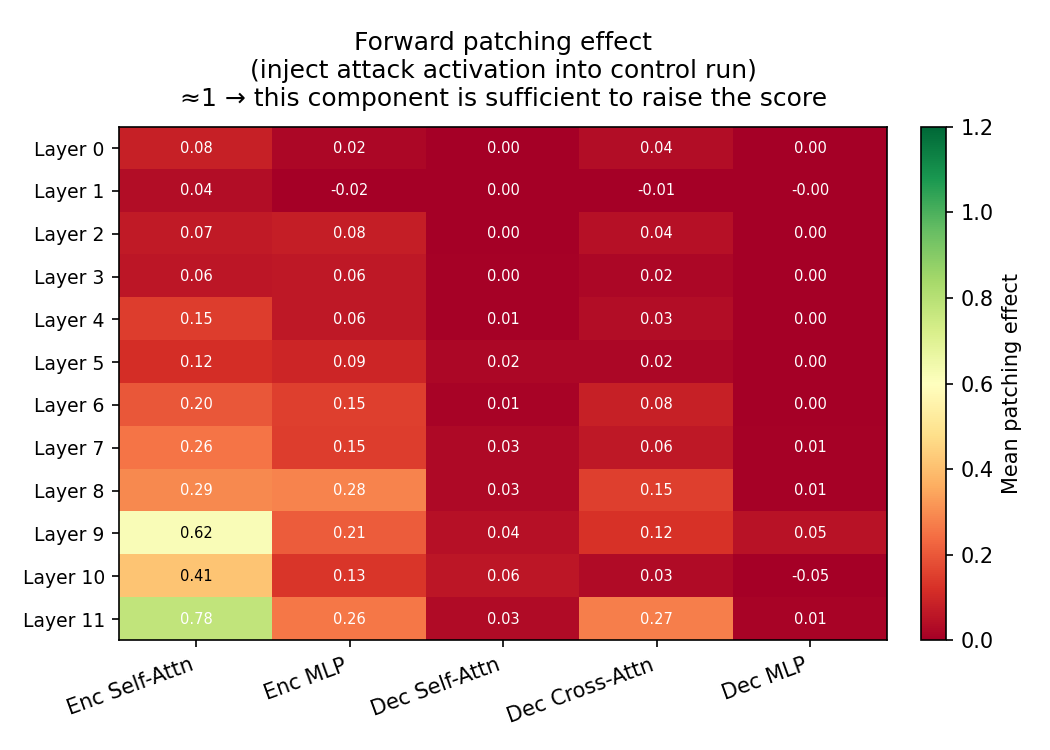
\includegraphics[width=0.17\textwidth]{outputs/attacks/bar_random_1/plots/forward_layer_component_heatmap.png} & 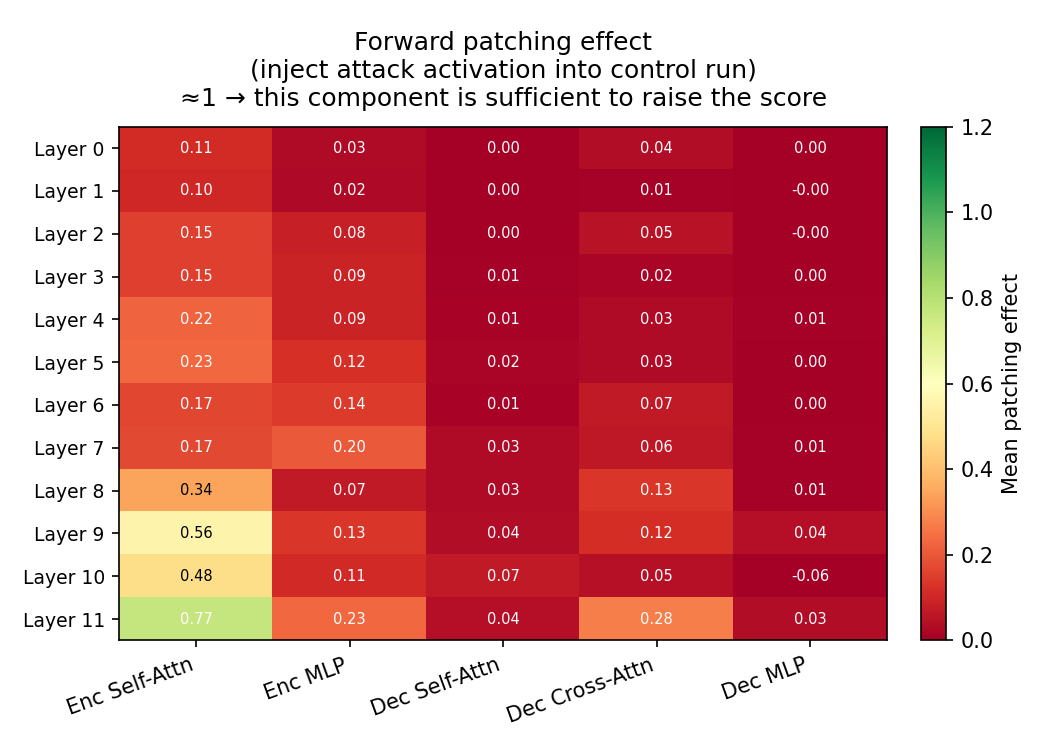
\includegraphics[width=0.17\textwidth]{outputs/attacks/bar_random_2/plots/forward_layer_component_heatmap.png} & 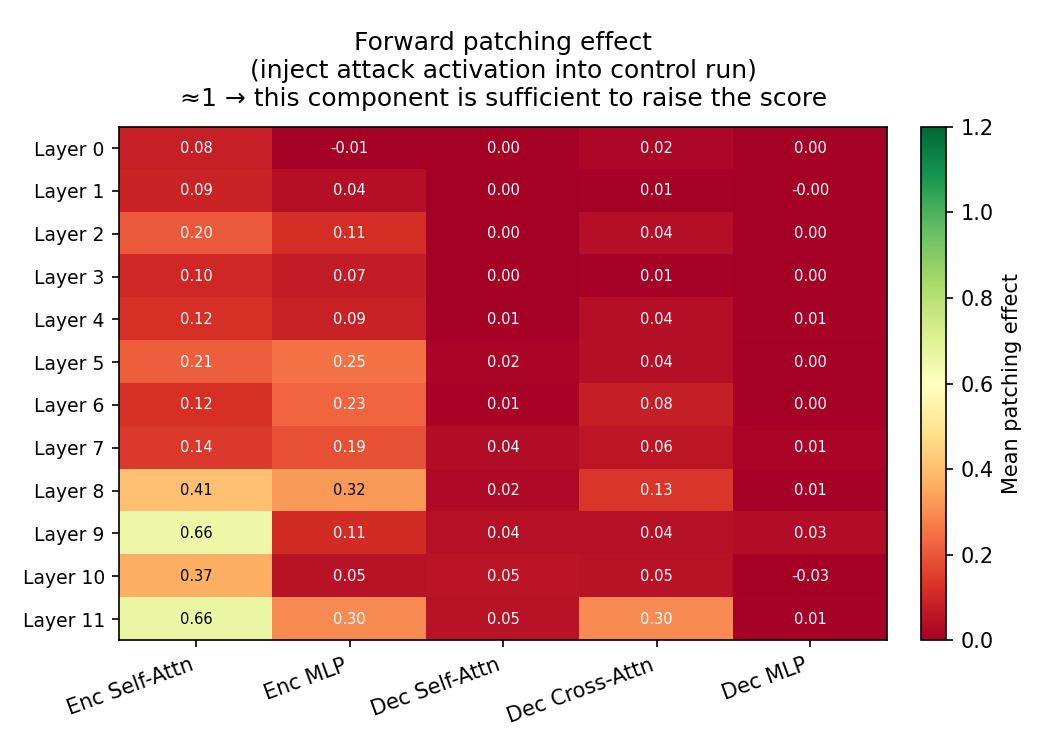
\includegraphics[width=0.17\textwidth]{outputs/attacks/bar_random_3/plots/forward_layer_component_heatmap.png} & 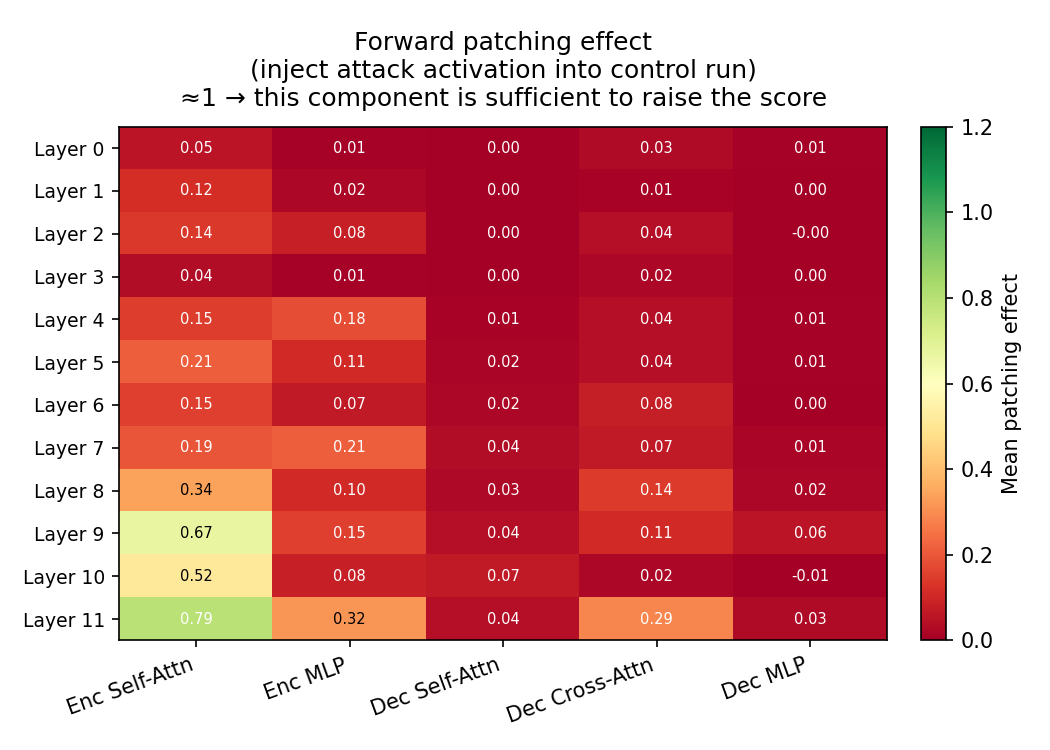
\includegraphics[width=0.17\textwidth]{outputs/attacks/bar_random_4/plots/forward_layer_component_heatmap.png} & 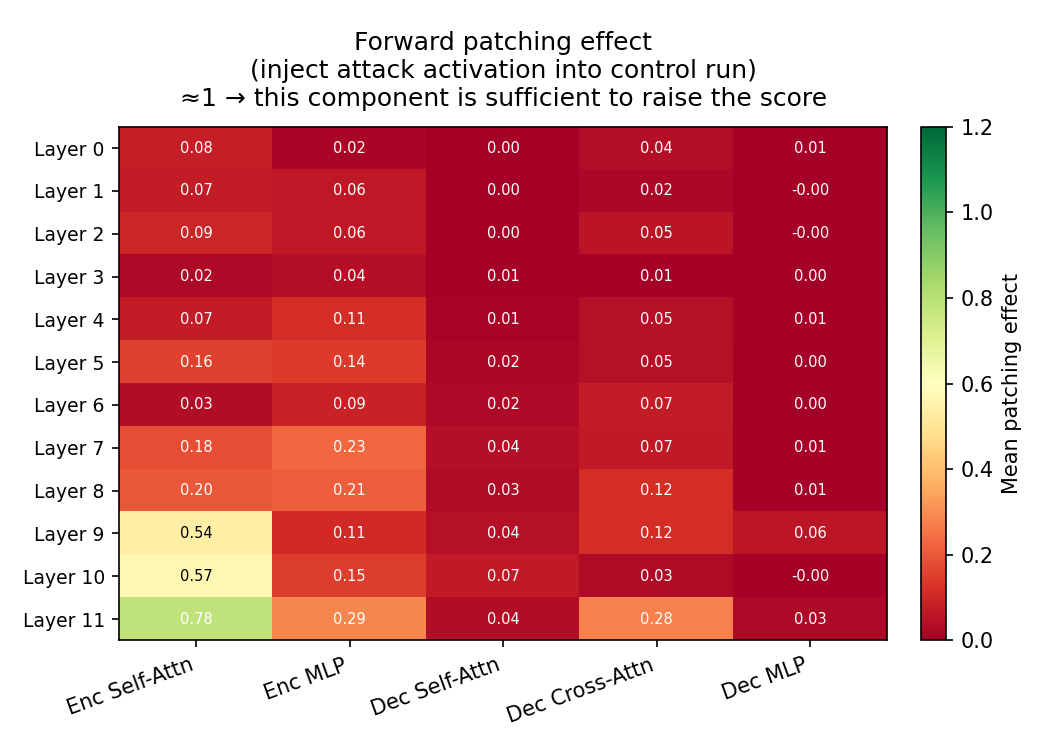
\includegraphics[width=0.17\textwidth]{outputs/attacks/bar_random_5/plots/forward_layer_component_heatmap.png} \\[4pt]
\rotatebox{90}{\textbf{reverse}} & 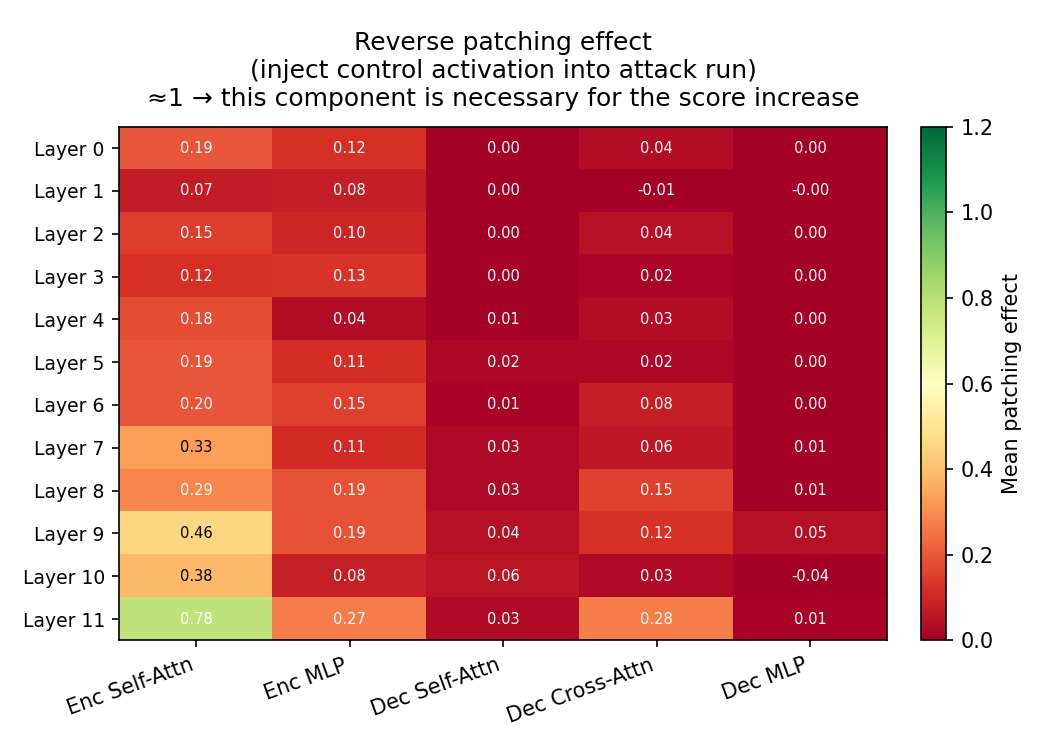
\includegraphics[width=0.17\textwidth]{outputs/attacks/bar_random_1/plots/reverse_layer_component_heatmap.png} & 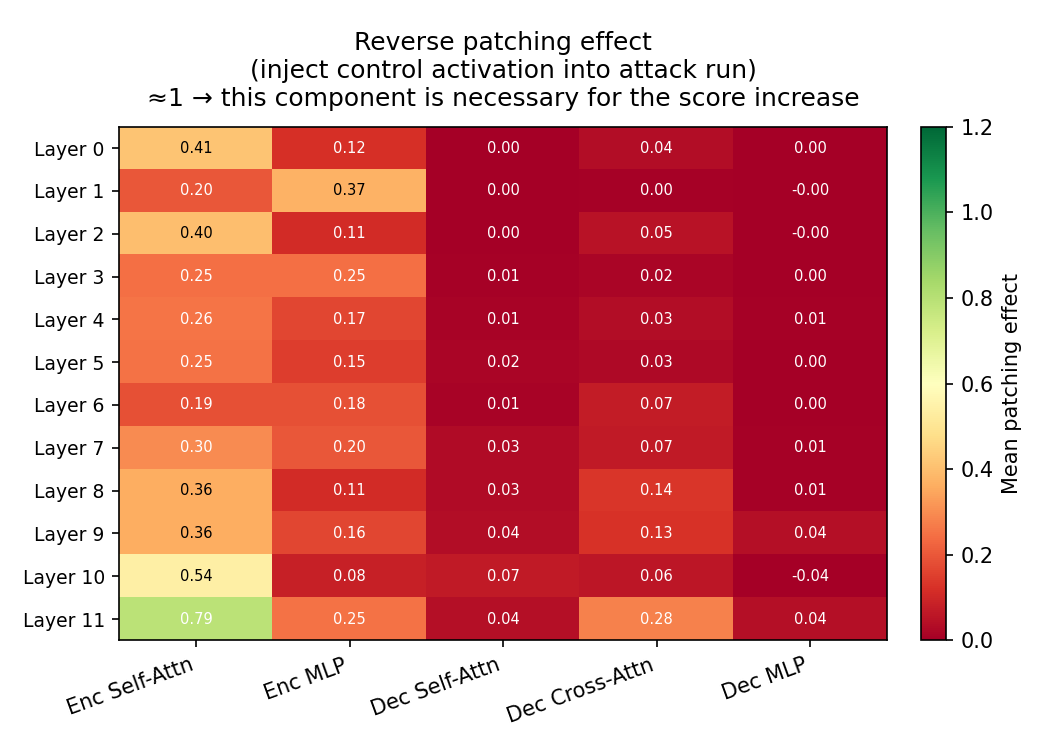
\includegraphics[width=0.17\textwidth]{outputs/attacks/bar_random_2/plots/reverse_layer_component_heatmap.png} & 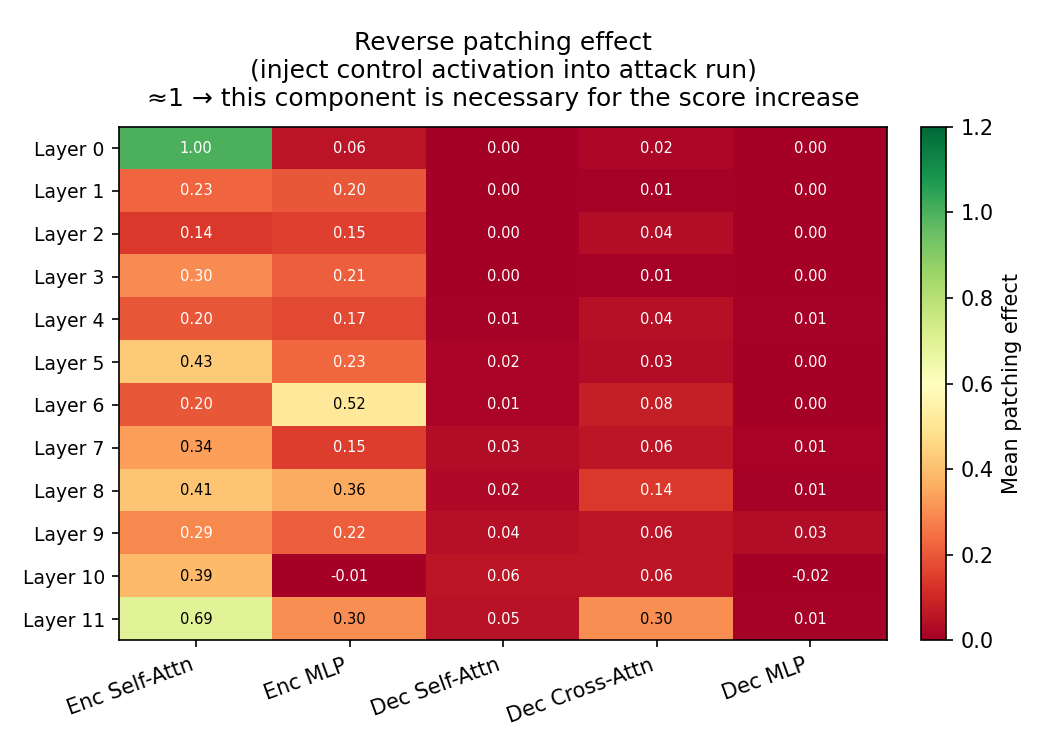
\includegraphics[width=0.17\textwidth]{outputs/attacks/bar_random_3/plots/reverse_layer_component_heatmap.png} & 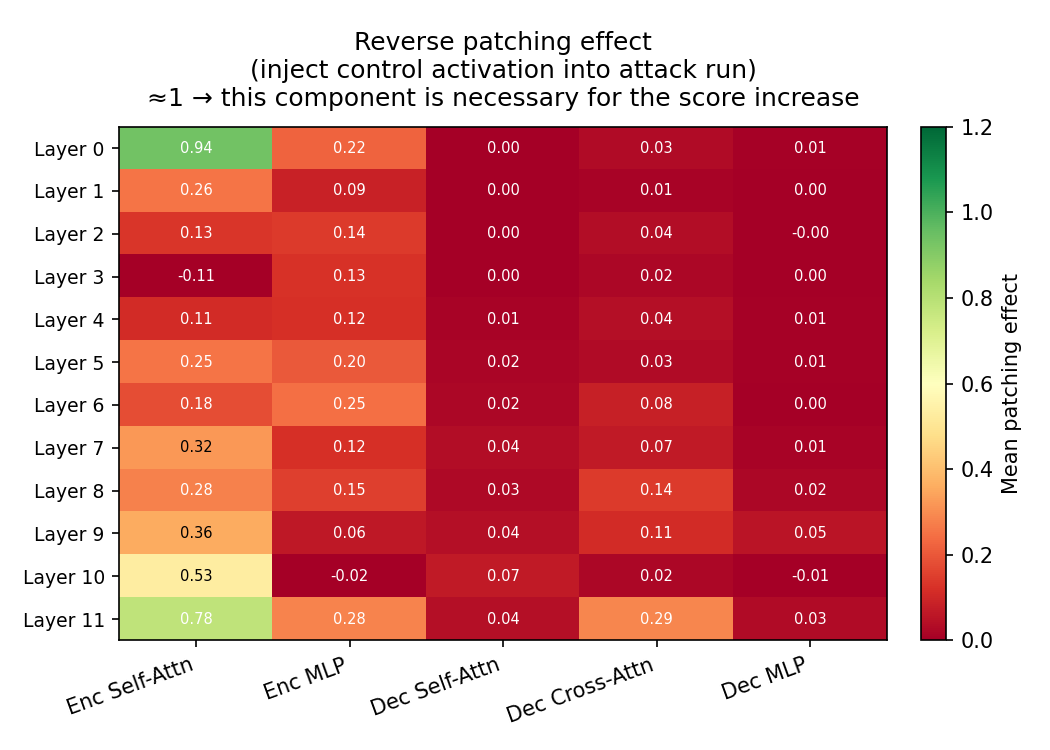
\includegraphics[width=0.17\textwidth]{outputs/attacks/bar_random_4/plots/reverse_layer_component_heatmap.png} & 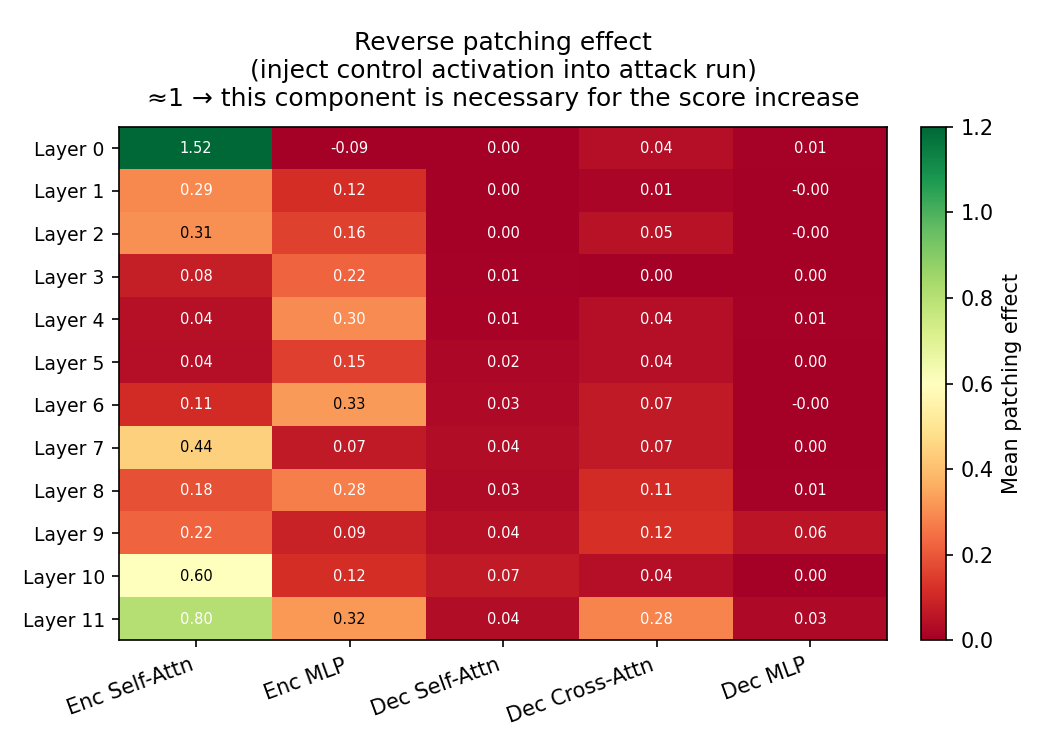
\includegraphics[width=0.17\textwidth]{outputs/attacks/bar_random_5/plots/reverse_layer_component_heatmap.png} \\[4pt]
\rotatebox{90}{\textbf{combined}} & 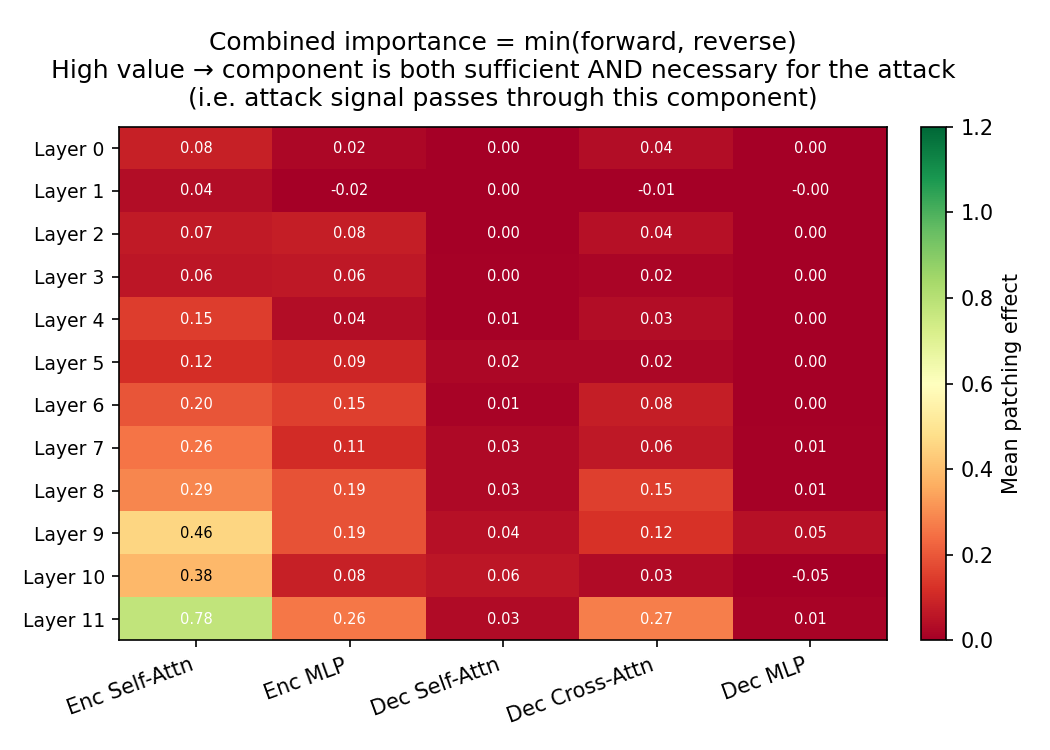
\includegraphics[width=0.17\textwidth]{outputs/attacks/bar_random_1/plots/combined_layer_component_heatmap.png} & 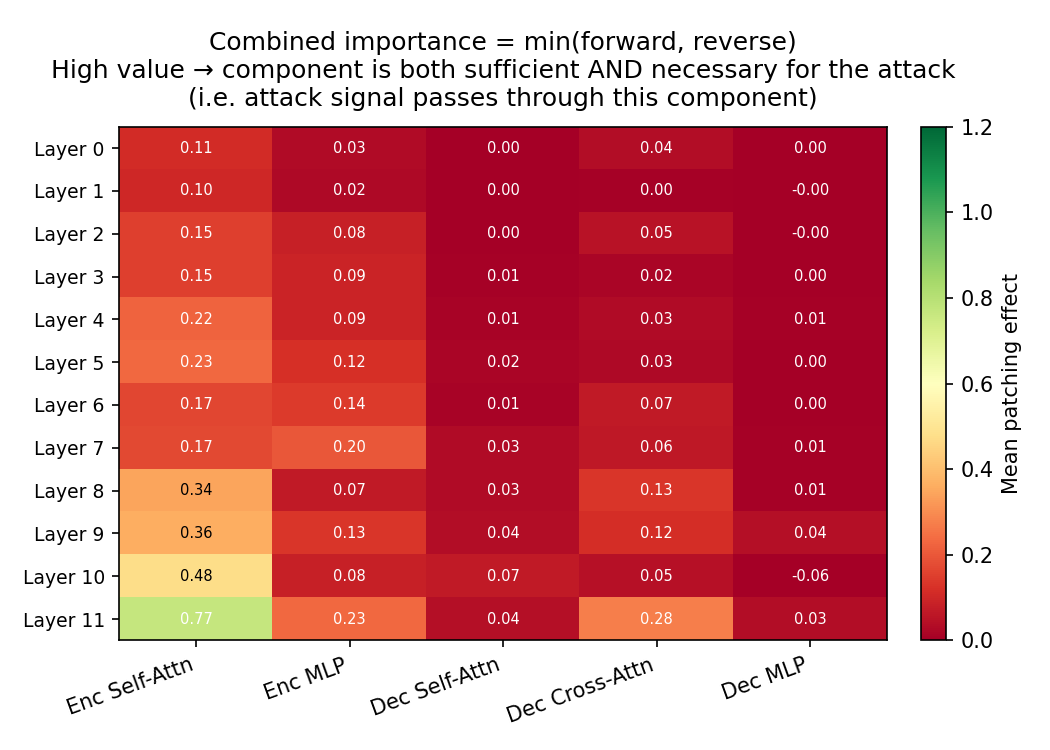
\includegraphics[width=0.17\textwidth]{outputs/attacks/bar_random_2/plots/combined_layer_component_heatmap.png} & 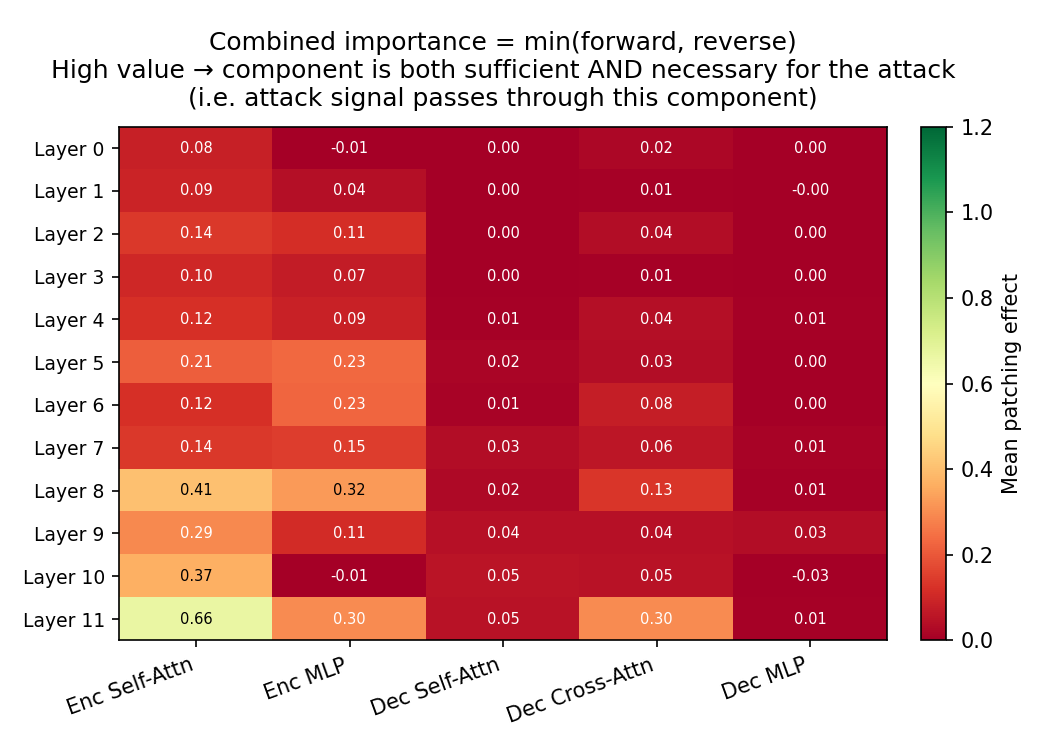
\includegraphics[width=0.17\textwidth]{outputs/attacks/bar_random_3/plots/combined_layer_component_heatmap.png} & 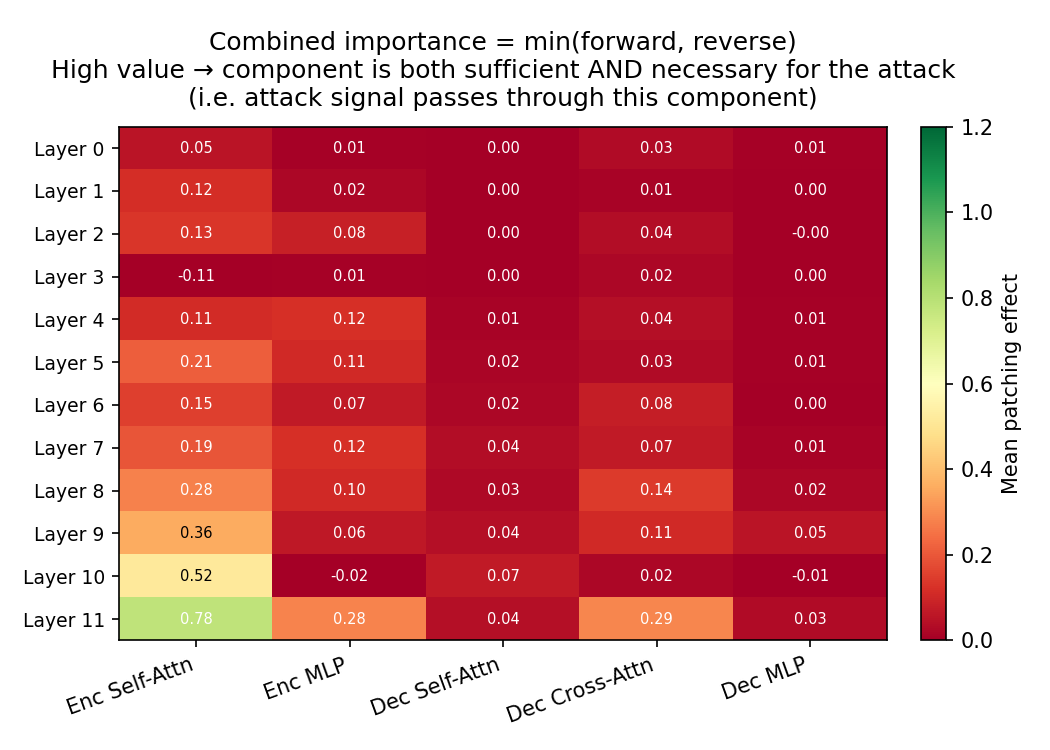
\includegraphics[width=0.17\textwidth]{outputs/attacks/bar_random_4/plots/combined_layer_component_heatmap.png} & 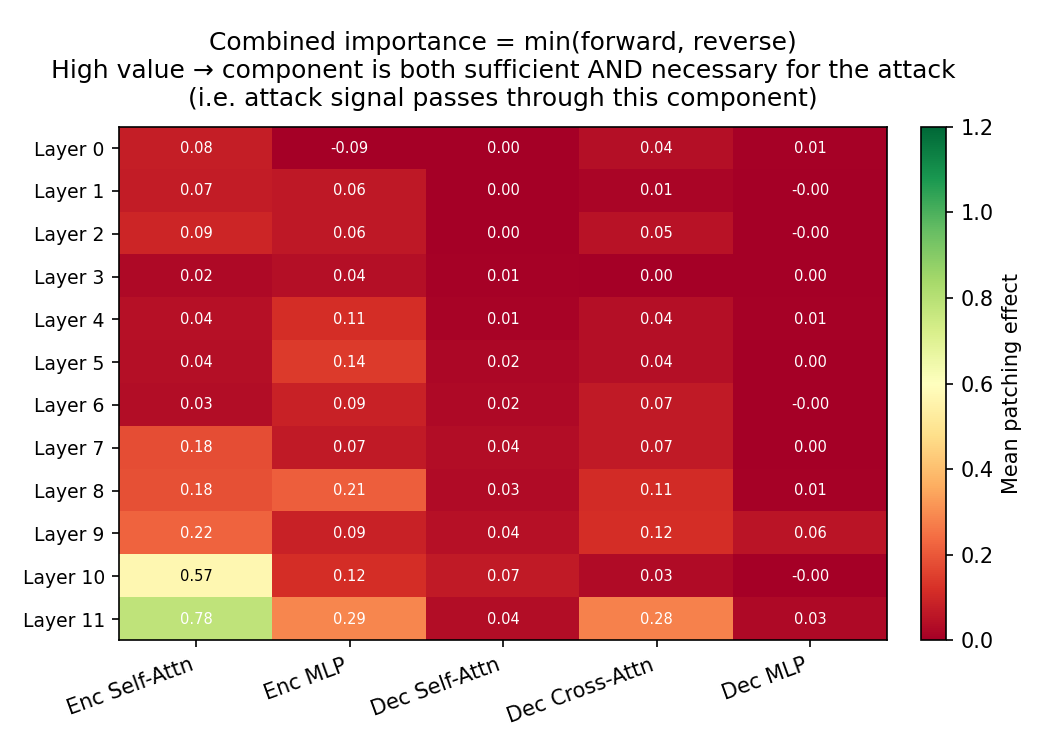
\includegraphics[width=0.17\textwidth]{outputs/attacks/bar_random_5/plots/combined_layer_component_heatmap.png} \\[4pt]
\end{tabular}
\caption{Patching heatmaps for \texttt{bar_random}: forward (top), reverse (middle), combined (bottom) across repetitions 1--5.}
\label{fig:hm:bar_random}
\end{figure}

\begin{figure}[H]
\centering
\setlength{\tabcolsep}{2pt}
\renewcommand{\arraystretch}{0.5}
\begin{tabular}{r ccccc}
& \textbf{rep=1} & \textbf{rep=2} & \textbf{rep=3} & \textbf{rep=4} & \textbf{rep=5} \\[2pt]
\rotatebox{90}{\textbf{forward}} & 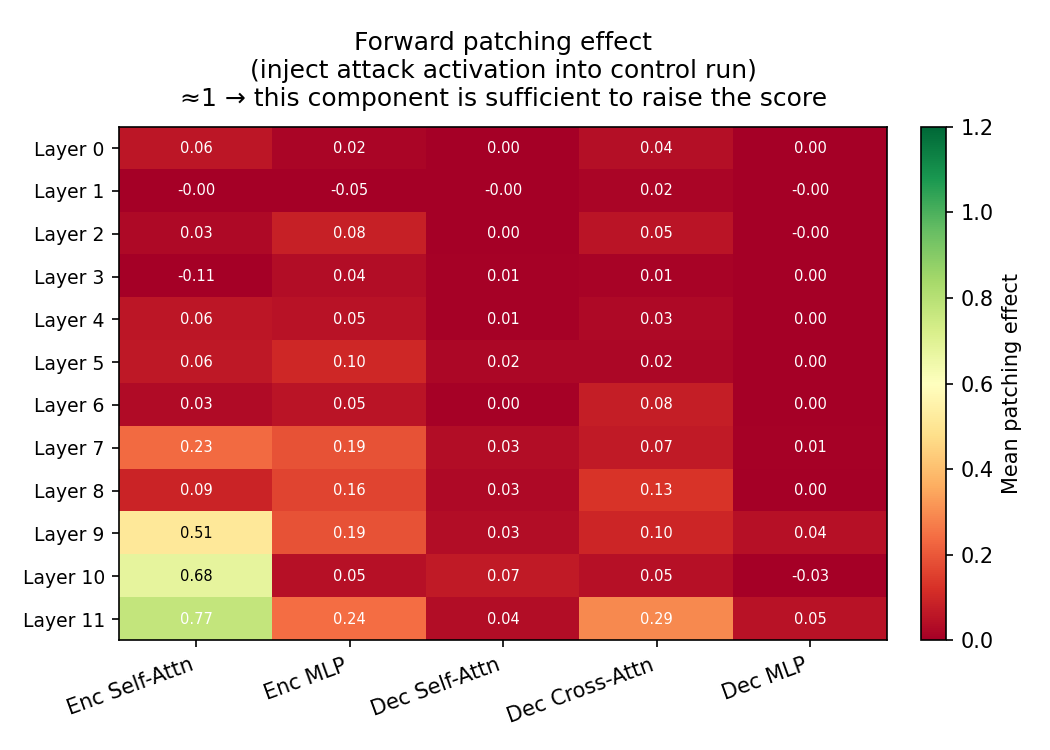
\includegraphics[width=0.17\textwidth]{outputs/attacks/bar_start_1/plots/forward_layer_component_heatmap.png} & 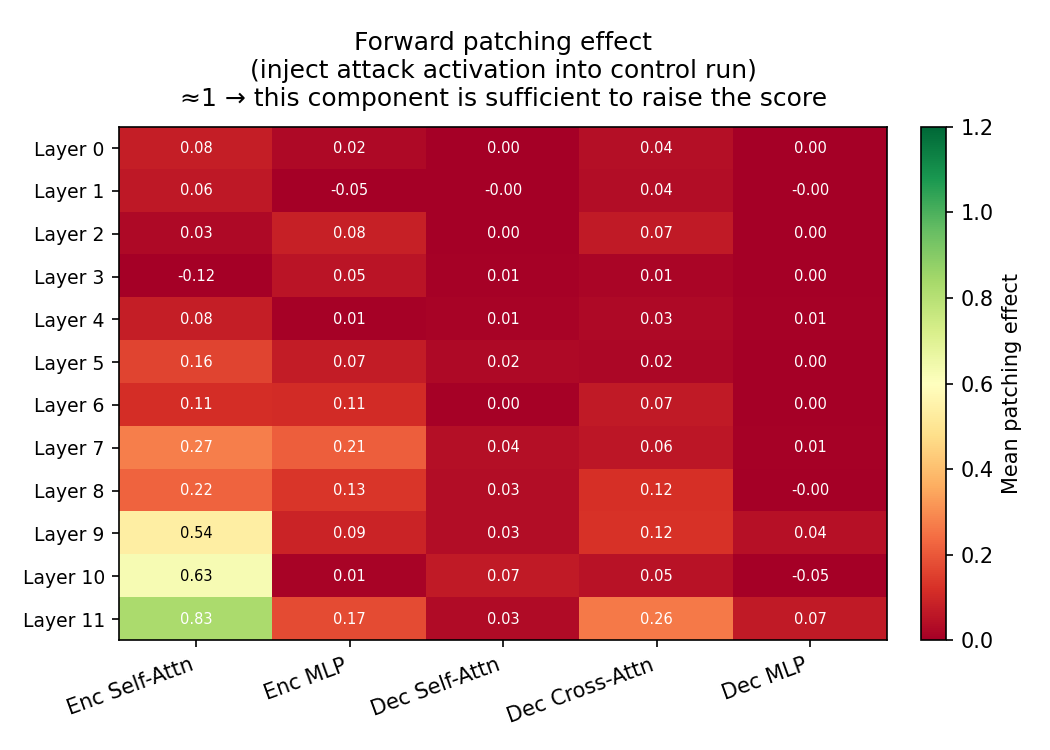
\includegraphics[width=0.17\textwidth]{outputs/attacks/bar_start_2/plots/forward_layer_component_heatmap.png} & 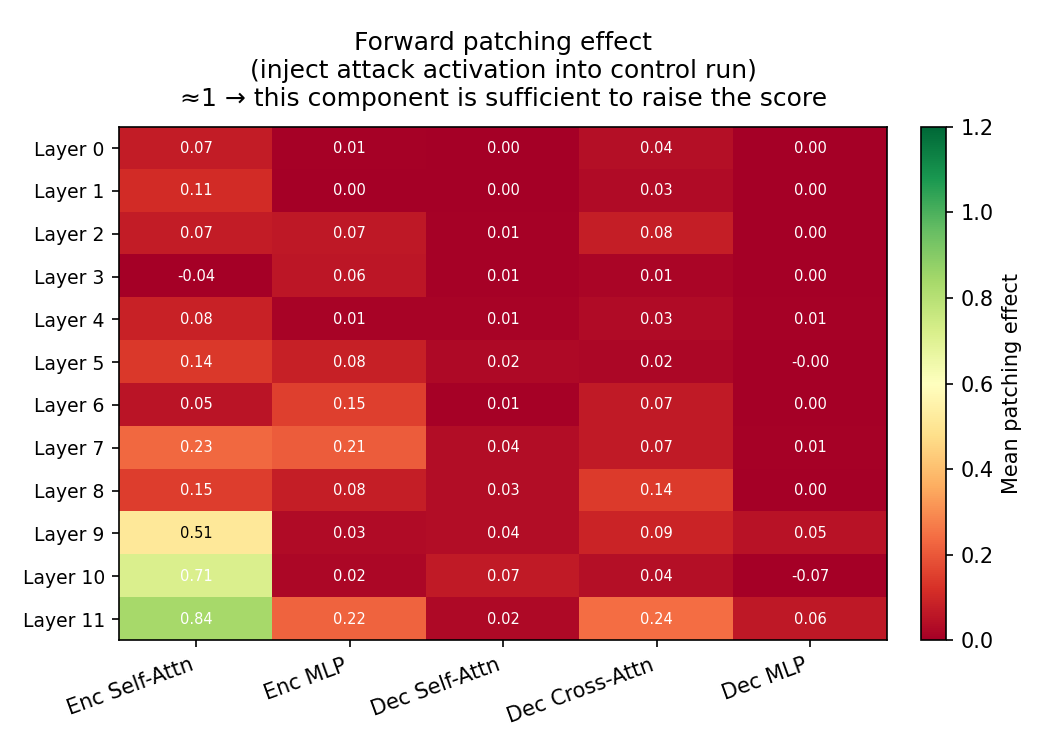
\includegraphics[width=0.17\textwidth]{outputs/attacks/bar_start_3/plots/forward_layer_component_heatmap.png} & 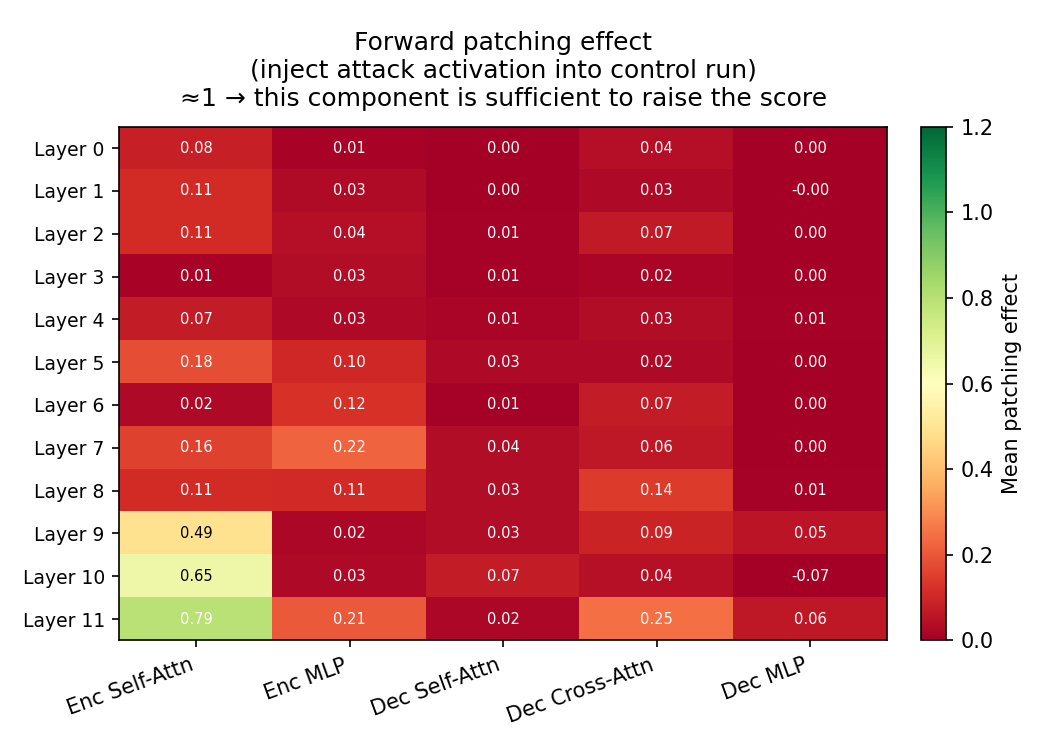
\includegraphics[width=0.17\textwidth]{outputs/attacks/bar_start_4/plots/forward_layer_component_heatmap.png} & 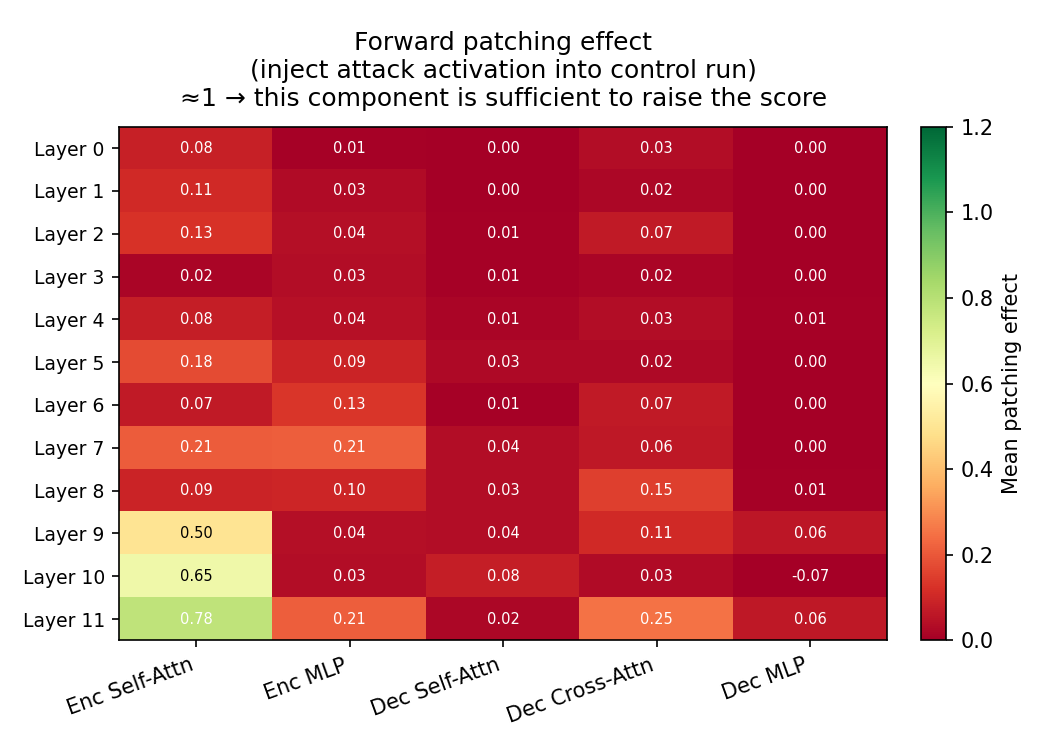
\includegraphics[width=0.17\textwidth]{outputs/attacks/bar_start_5/plots/forward_layer_component_heatmap.png} \\[4pt]
\rotatebox{90}{\textbf{reverse}} & 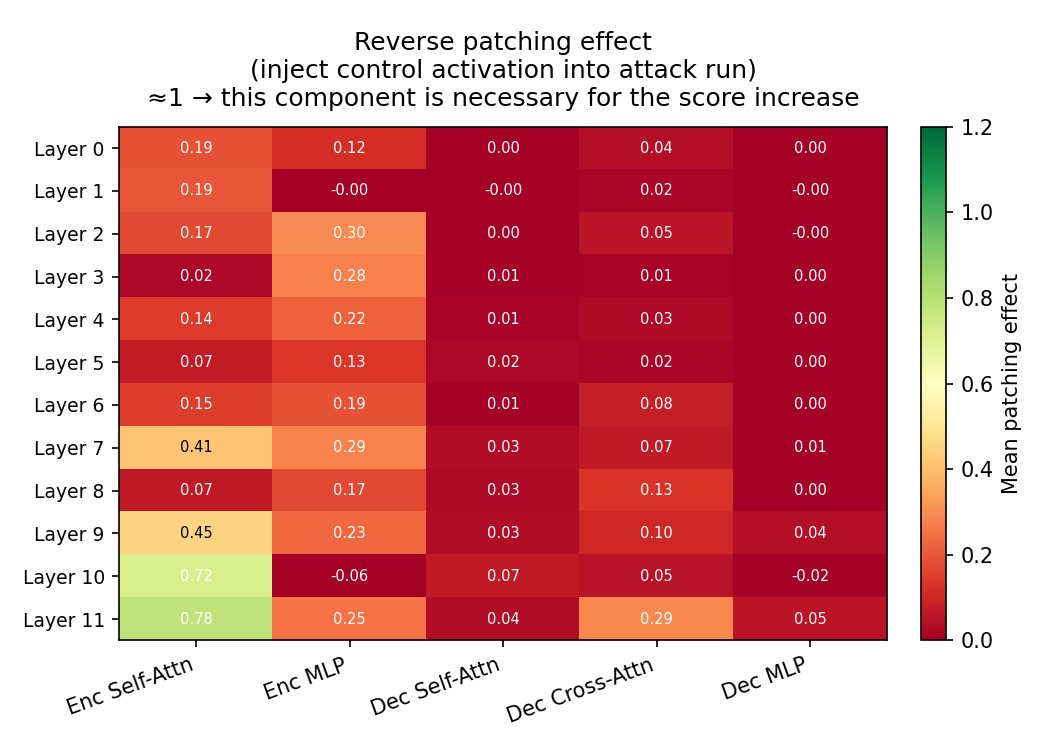
\includegraphics[width=0.17\textwidth]{outputs/attacks/bar_start_1/plots/reverse_layer_component_heatmap.png} & 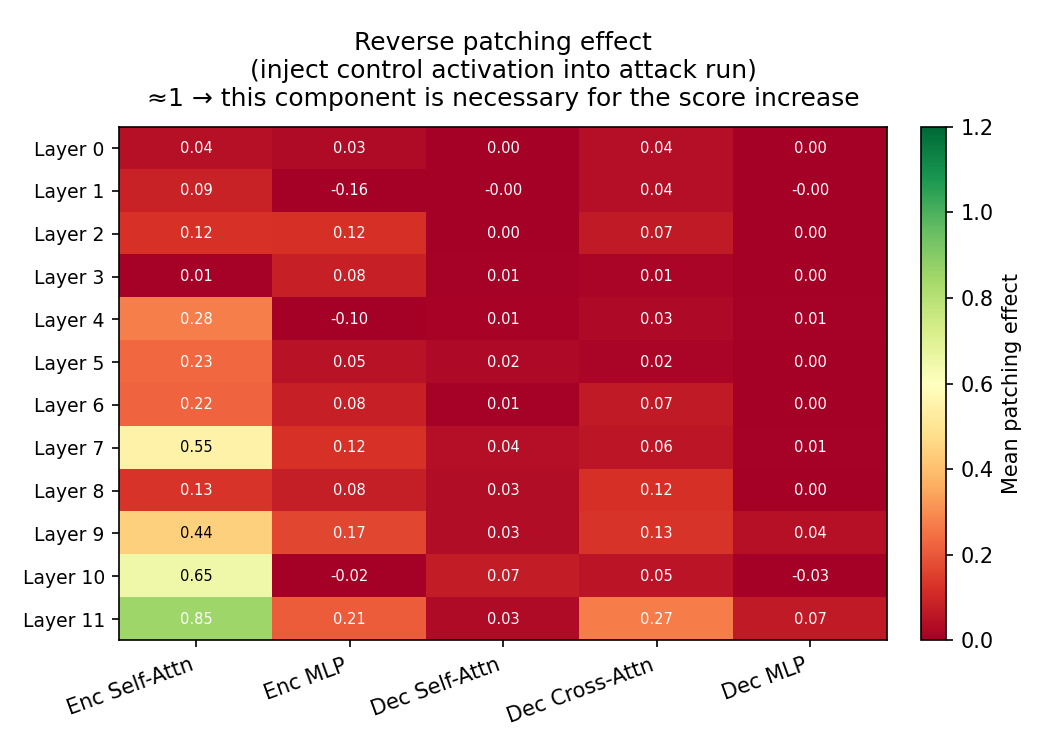
\includegraphics[width=0.17\textwidth]{outputs/attacks/bar_start_2/plots/reverse_layer_component_heatmap.png} & 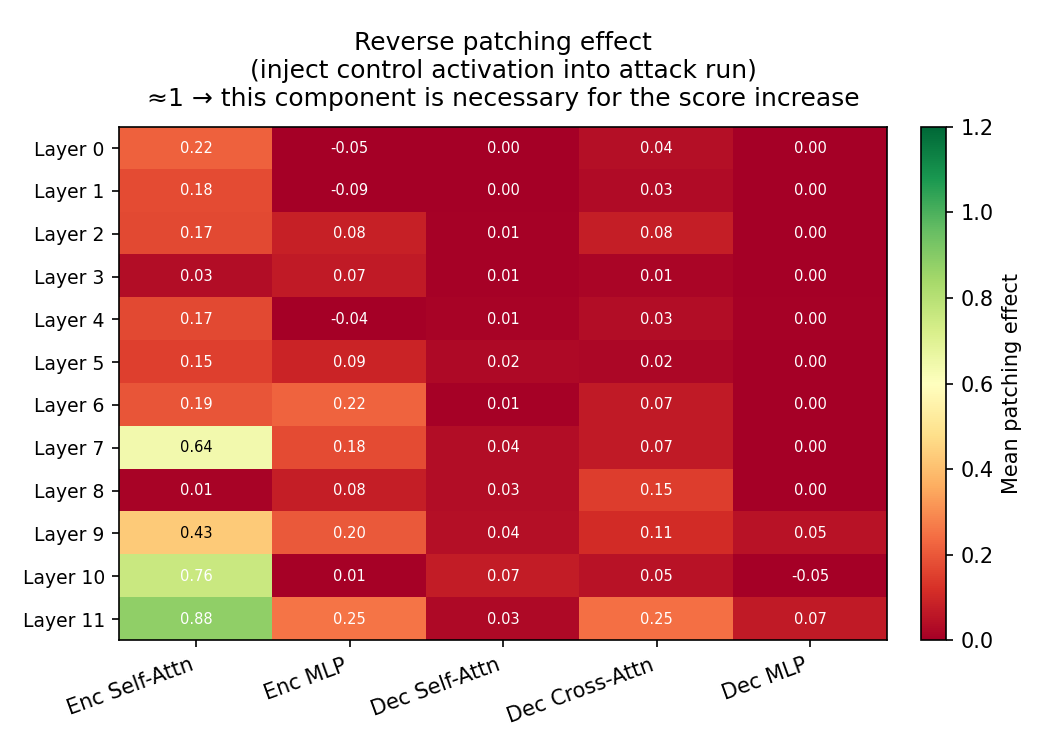
\includegraphics[width=0.17\textwidth]{outputs/attacks/bar_start_3/plots/reverse_layer_component_heatmap.png} & 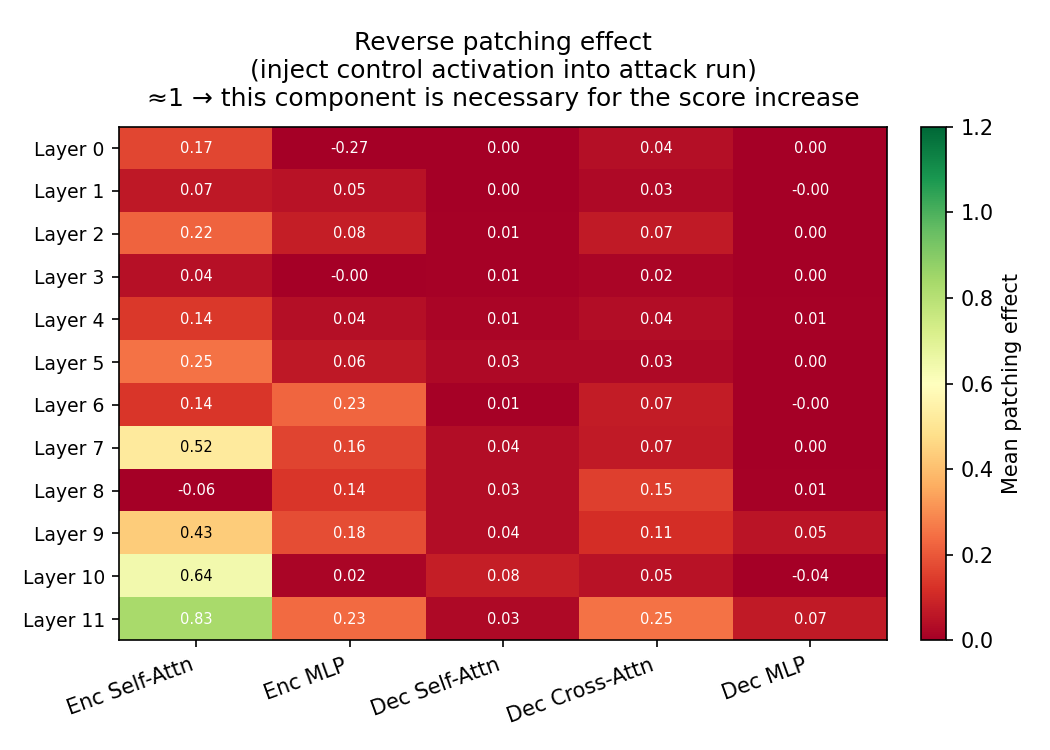
\includegraphics[width=0.17\textwidth]{outputs/attacks/bar_start_4/plots/reverse_layer_component_heatmap.png} & 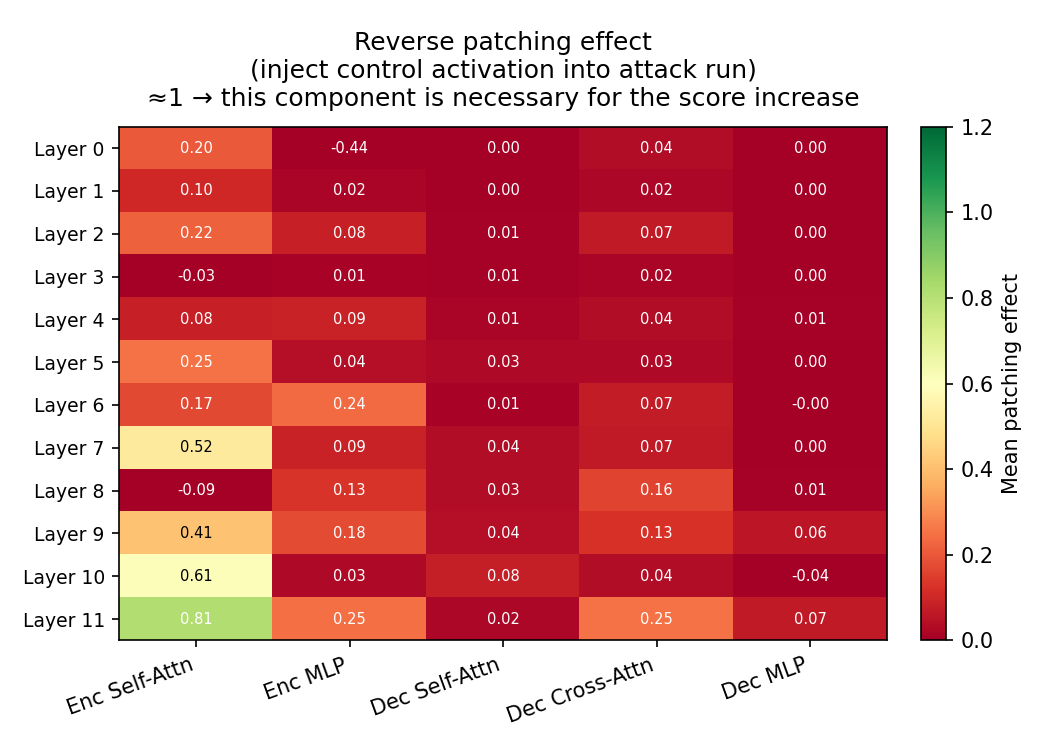
\includegraphics[width=0.17\textwidth]{outputs/attacks/bar_start_5/plots/reverse_layer_component_heatmap.png} \\[4pt]
\rotatebox{90}{\textbf{combined}} & 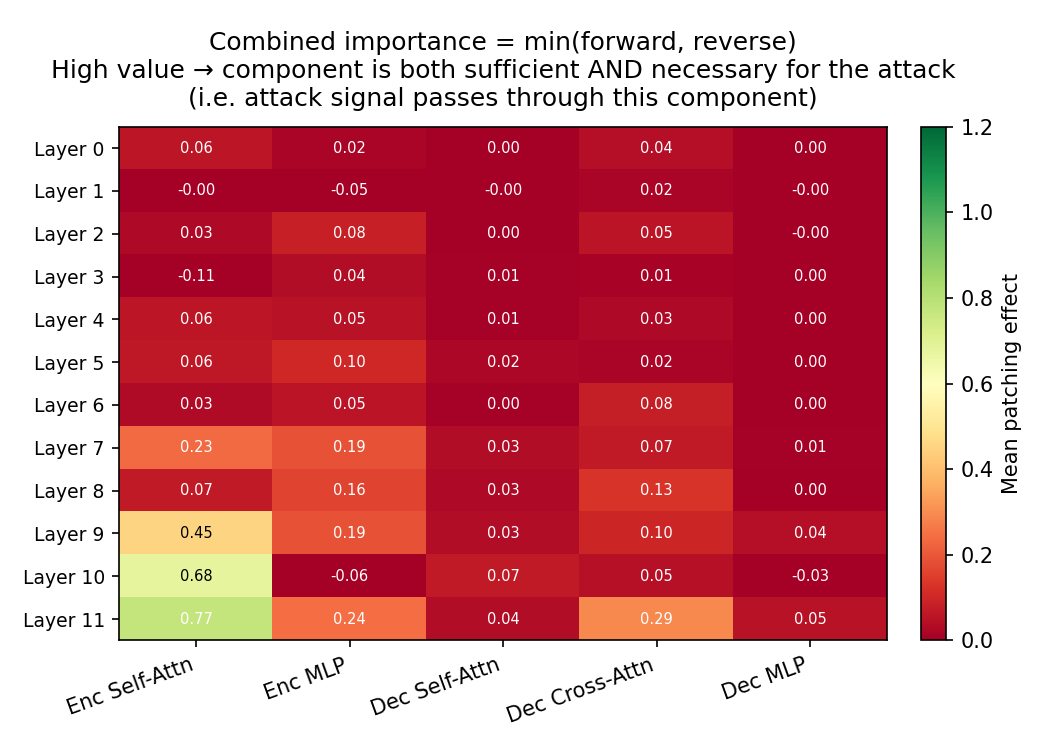
\includegraphics[width=0.17\textwidth]{outputs/attacks/bar_start_1/plots/combined_layer_component_heatmap.png} & 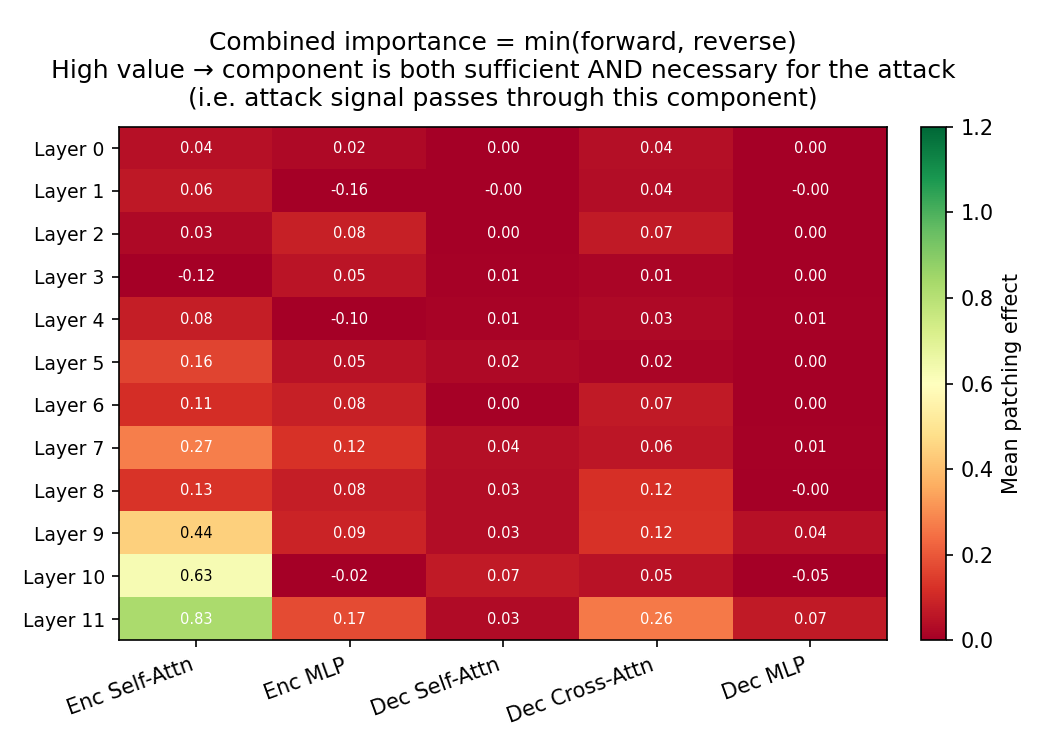
\includegraphics[width=0.17\textwidth]{outputs/attacks/bar_start_2/plots/combined_layer_component_heatmap.png} & 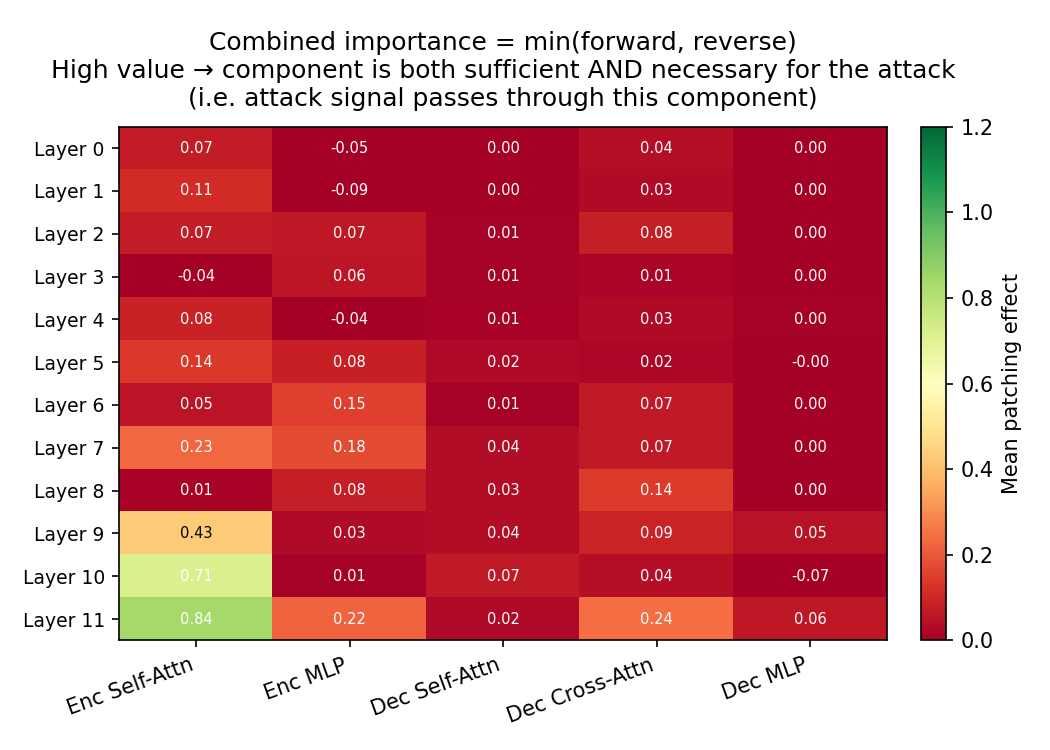
\includegraphics[width=0.17\textwidth]{outputs/attacks/bar_start_3/plots/combined_layer_component_heatmap.png} & 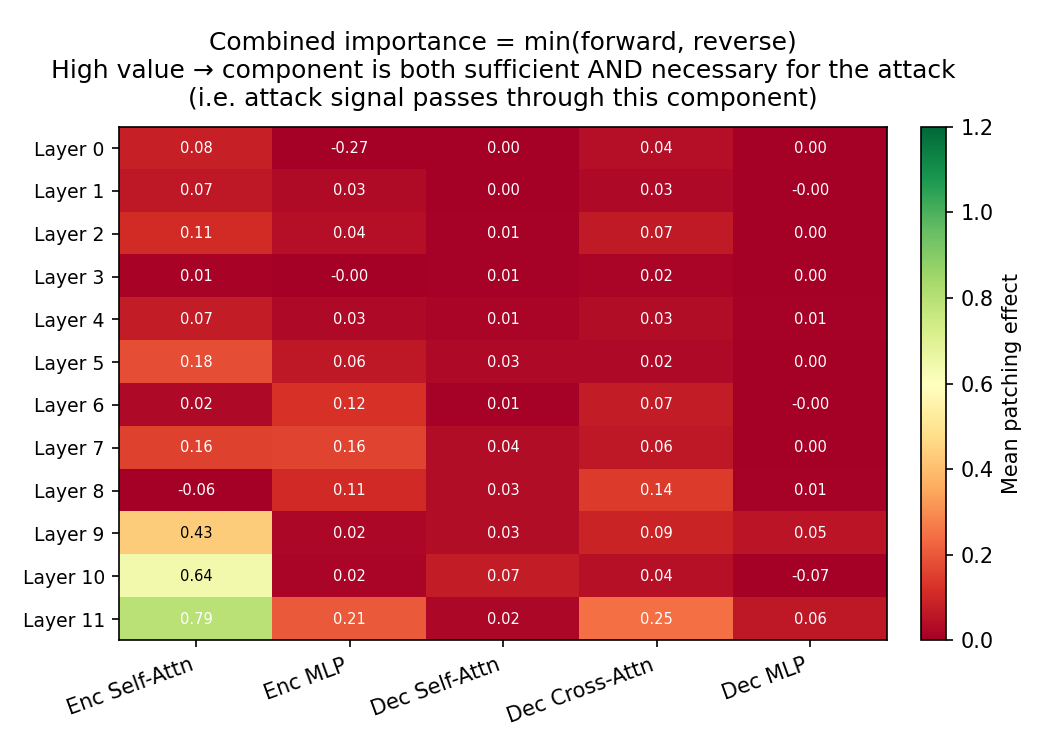
\includegraphics[width=0.17\textwidth]{outputs/attacks/bar_start_4/plots/combined_layer_component_heatmap.png} & 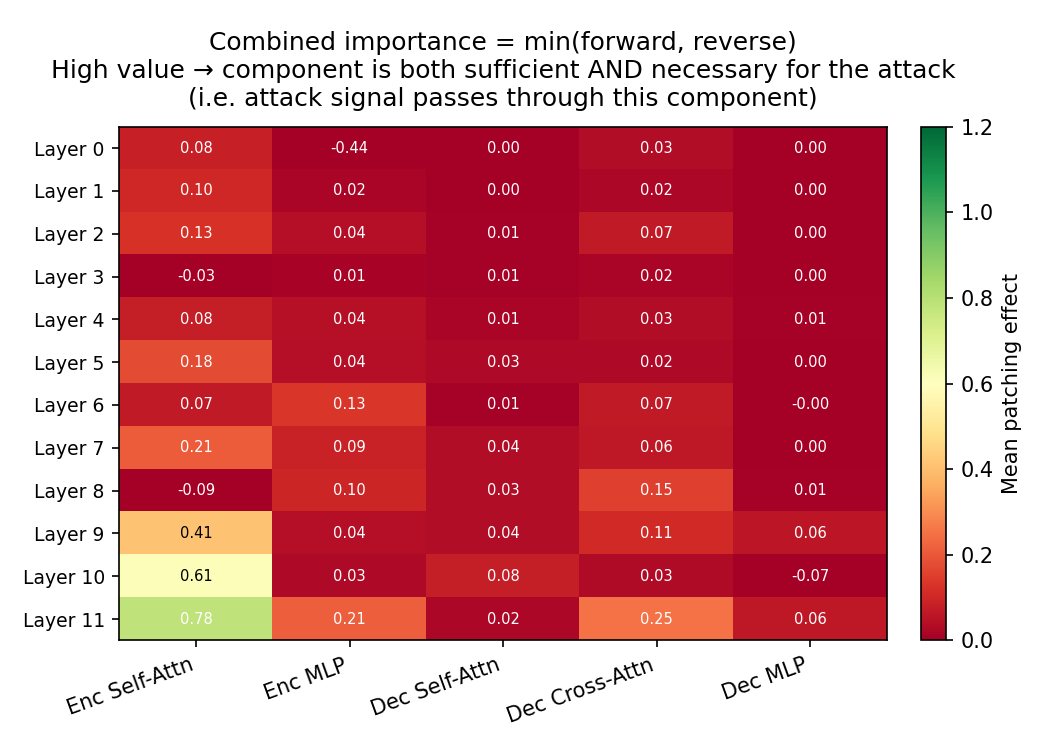
\includegraphics[width=0.17\textwidth]{outputs/attacks/bar_start_5/plots/combined_layer_component_heatmap.png} \\[4pt]
\end{tabular}
\caption{Patching heatmaps for \texttt{bar_start}: forward (top), reverse (middle), combined (bottom) across repetitions 1--5.}
\label{fig:hm:bar_start}
\end{figure}

\begin{figure}[H]
\centering
\setlength{\tabcolsep}{2pt}
\renewcommand{\arraystretch}{0.5}
\begin{tabular}{r ccccc}
& \textbf{rep=1} & \textbf{rep=2} & \textbf{rep=3} & \textbf{rep=4} & \textbf{rep=5} \\[2pt]
\rotatebox{90}{\textbf{forward}} & 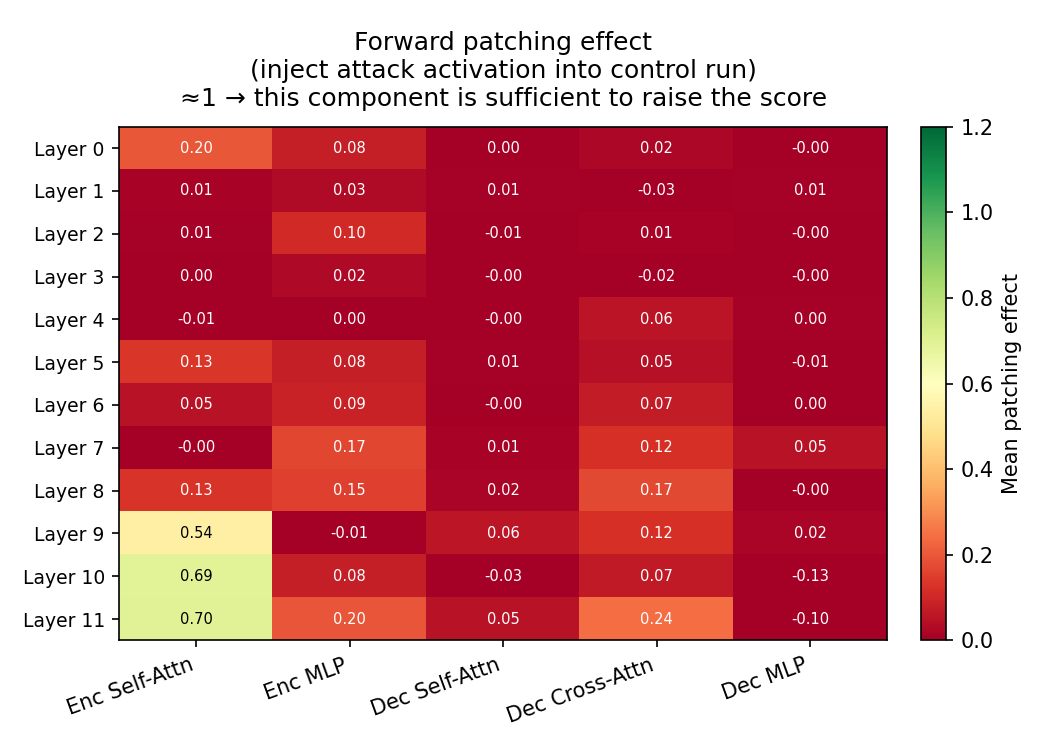
\includegraphics[width=0.17\textwidth]{outputs/attacks/false_end_1/plots/forward_layer_component_heatmap.png} & 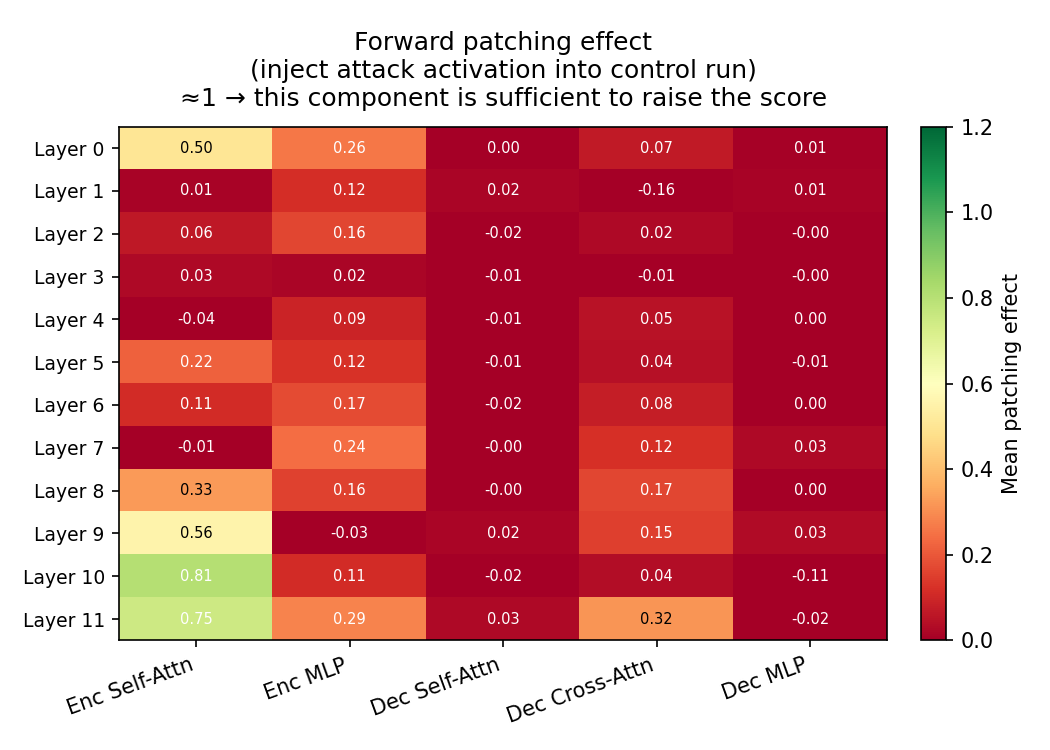
\includegraphics[width=0.17\textwidth]{outputs/attacks/false_end_2/plots/forward_layer_component_heatmap.png} & 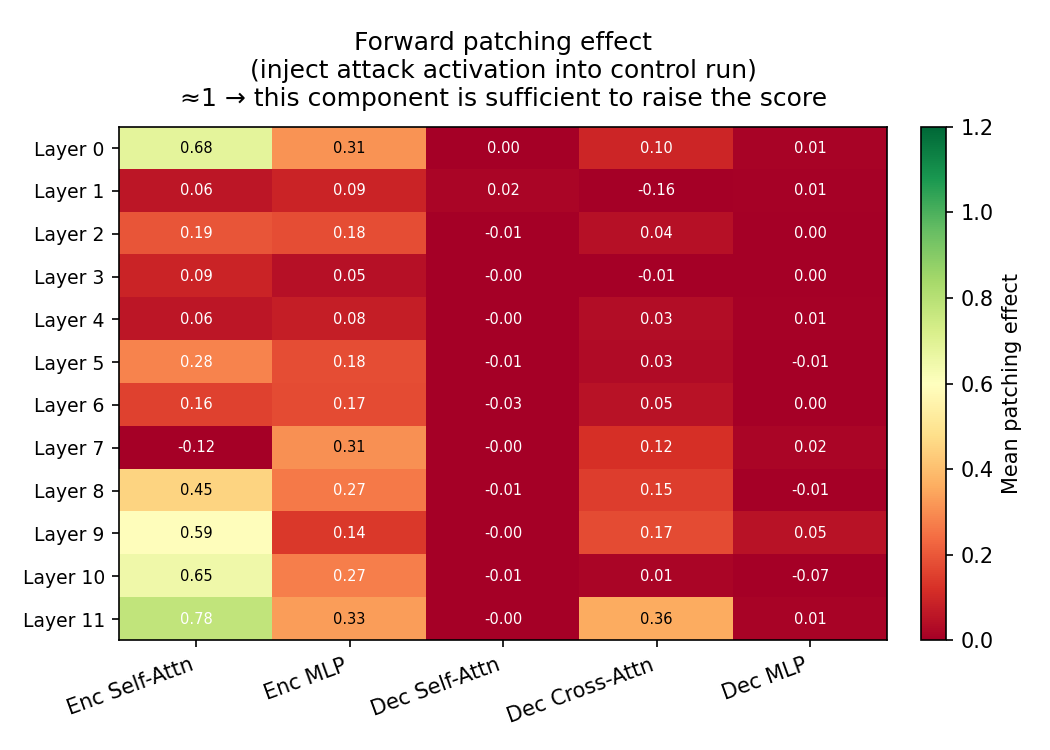
\includegraphics[width=0.17\textwidth]{outputs/attacks/false_end_3/plots/forward_layer_component_heatmap.png} & 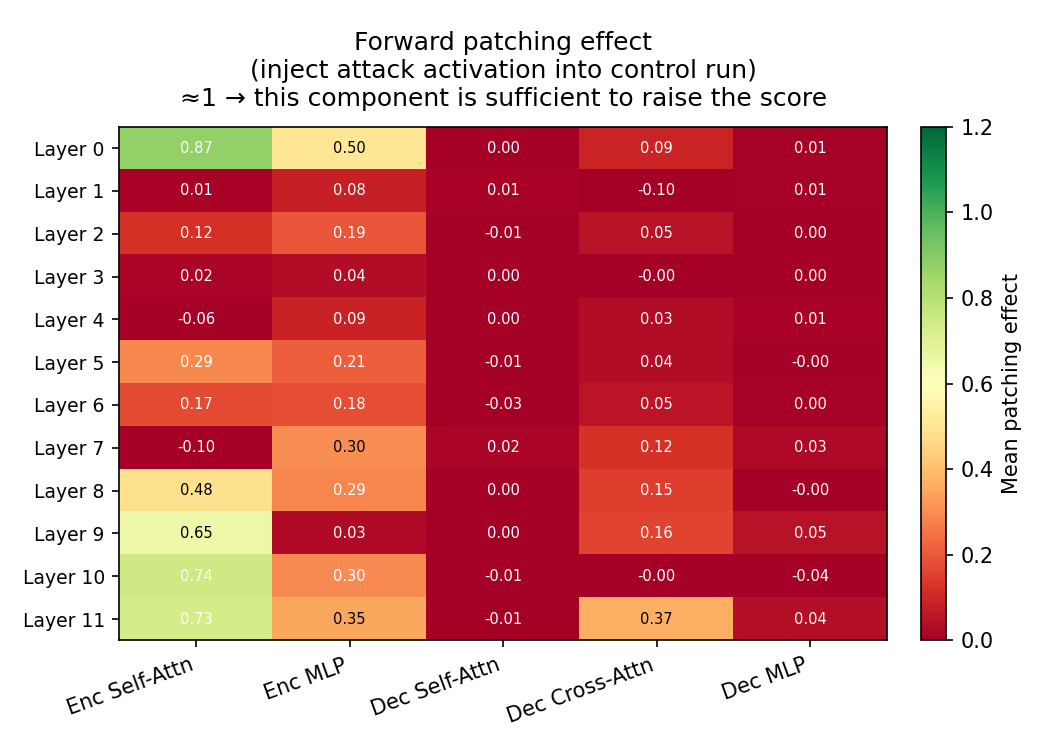
\includegraphics[width=0.17\textwidth]{outputs/attacks/false_end_4/plots/forward_layer_component_heatmap.png} & 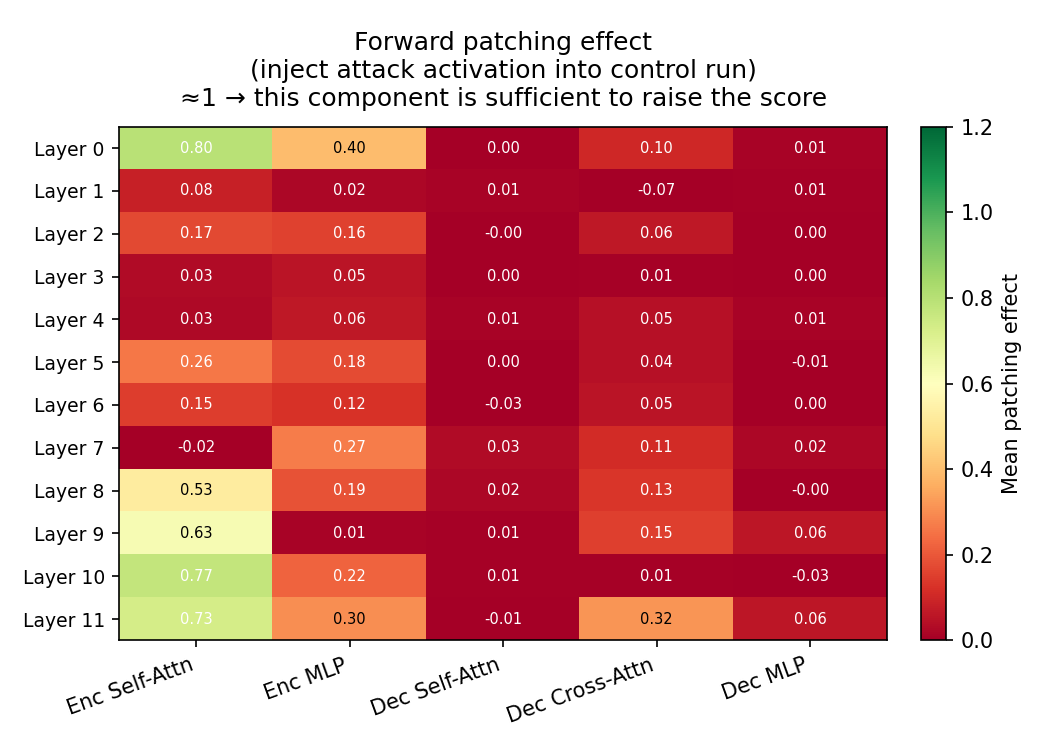
\includegraphics[width=0.17\textwidth]{outputs/attacks/false_end_5/plots/forward_layer_component_heatmap.png} \\[4pt]
\rotatebox{90}{\textbf{reverse}} & 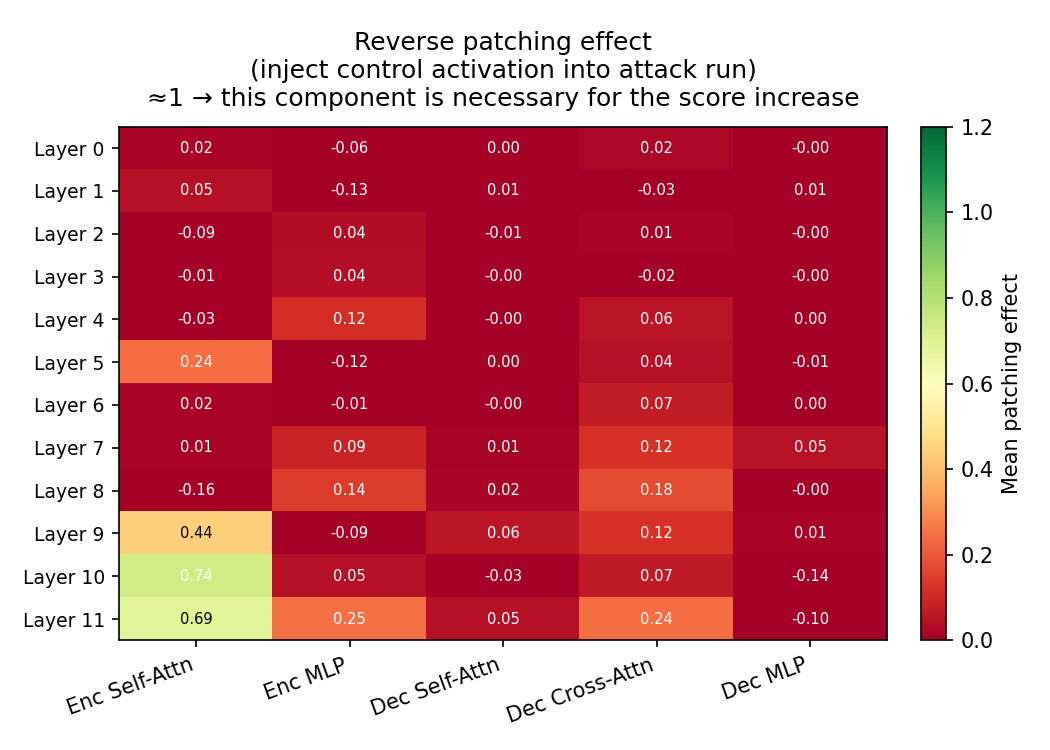
\includegraphics[width=0.17\textwidth]{outputs/attacks/false_end_1/plots/reverse_layer_component_heatmap.png} & 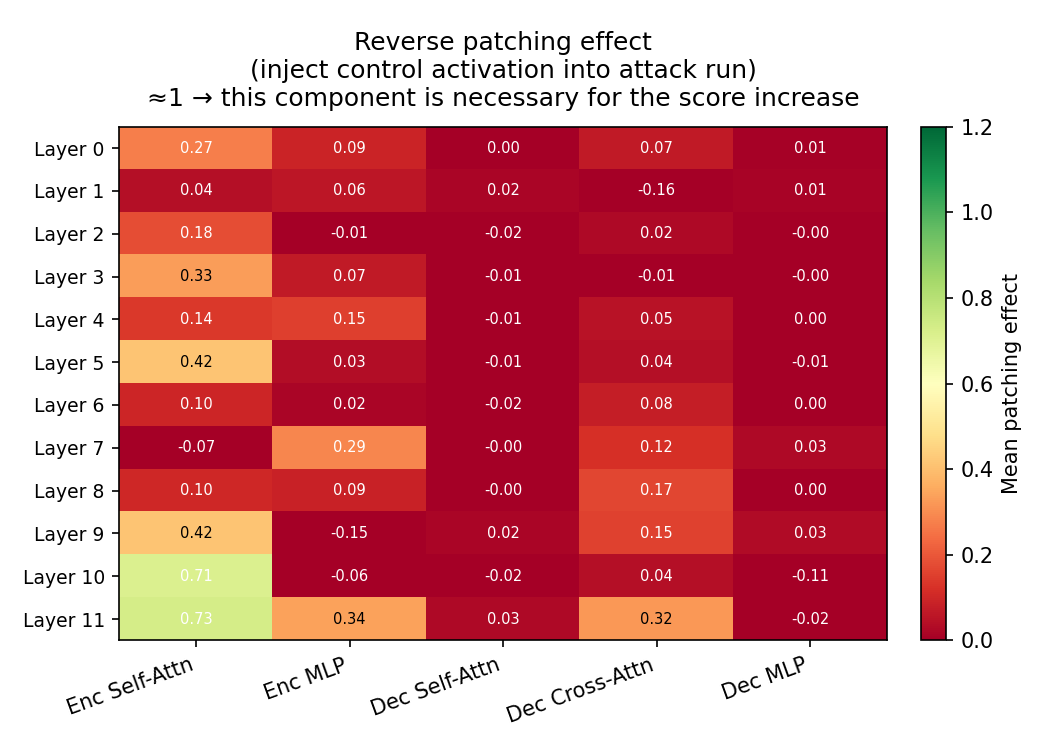
\includegraphics[width=0.17\textwidth]{outputs/attacks/false_end_2/plots/reverse_layer_component_heatmap.png} & 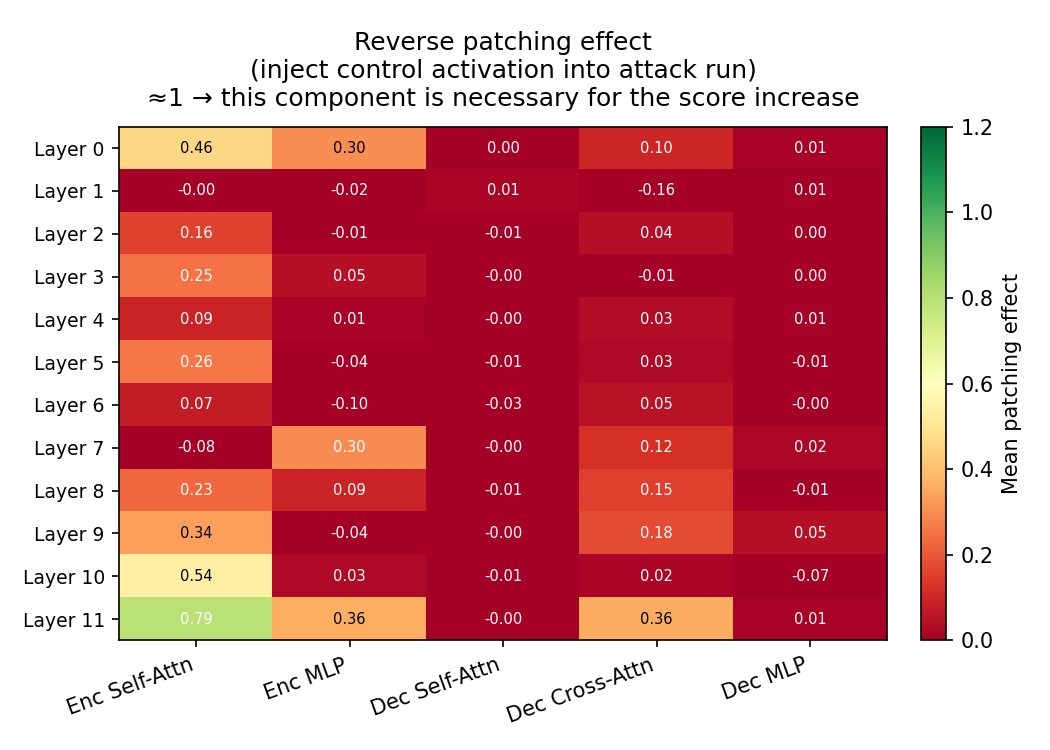
\includegraphics[width=0.17\textwidth]{outputs/attacks/false_end_3/plots/reverse_layer_component_heatmap.png} & 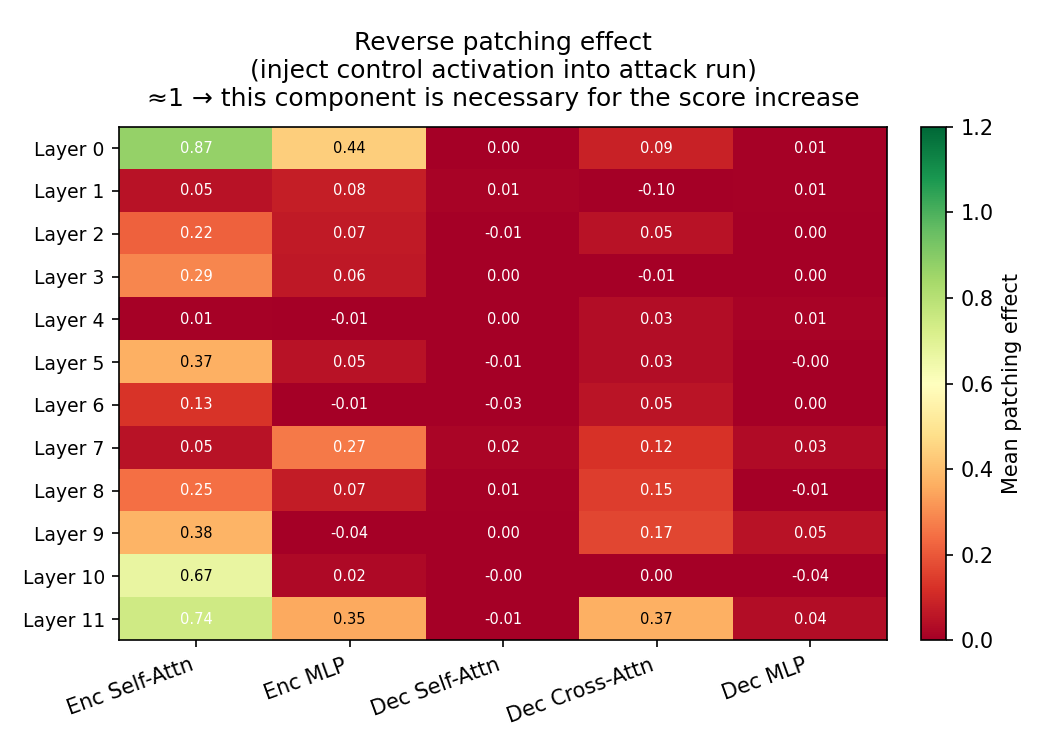
\includegraphics[width=0.17\textwidth]{outputs/attacks/false_end_4/plots/reverse_layer_component_heatmap.png} & 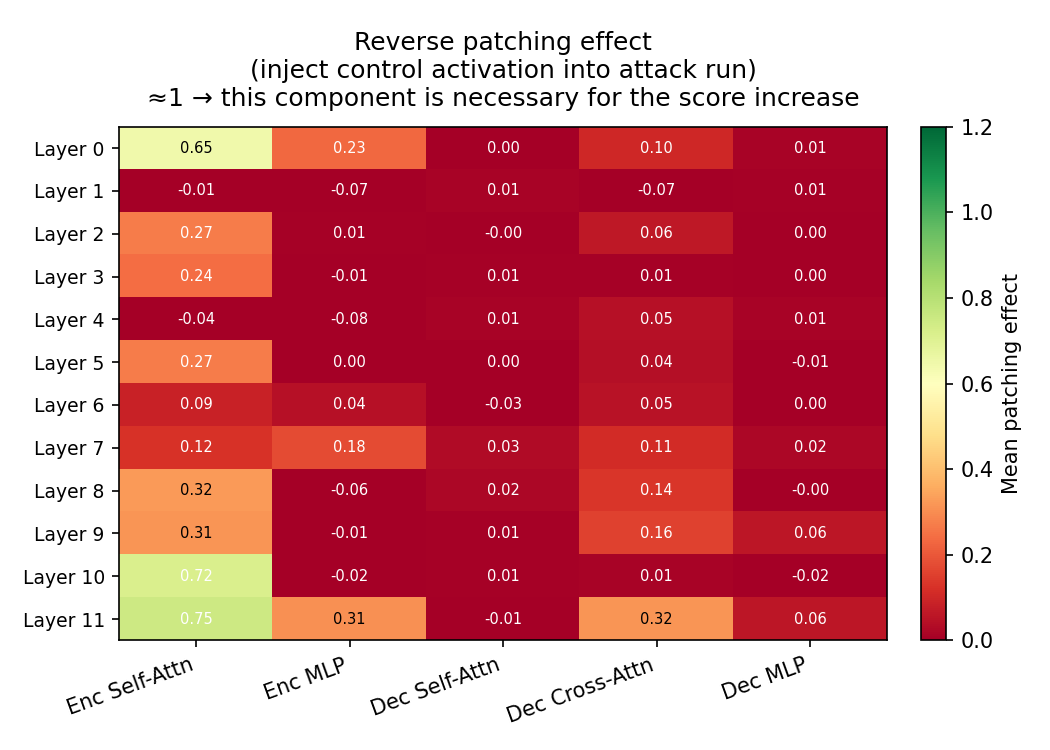
\includegraphics[width=0.17\textwidth]{outputs/attacks/false_end_5/plots/reverse_layer_component_heatmap.png} \\[4pt]
\rotatebox{90}{\textbf{combined}} & 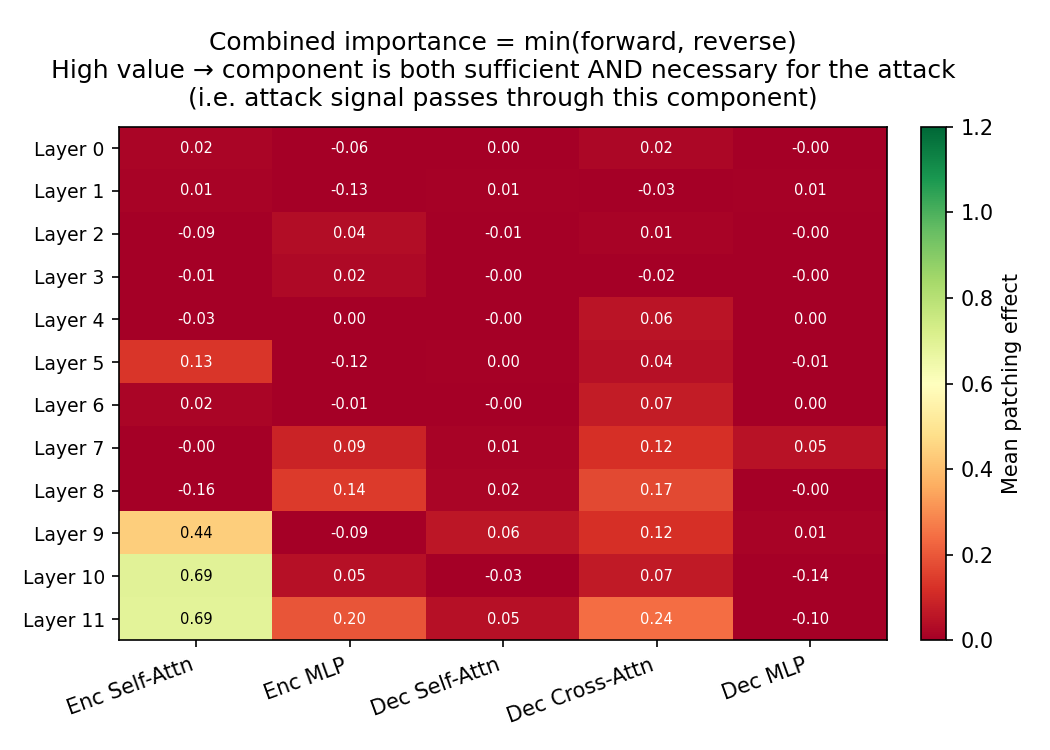
\includegraphics[width=0.17\textwidth]{outputs/attacks/false_end_1/plots/combined_layer_component_heatmap.png} & 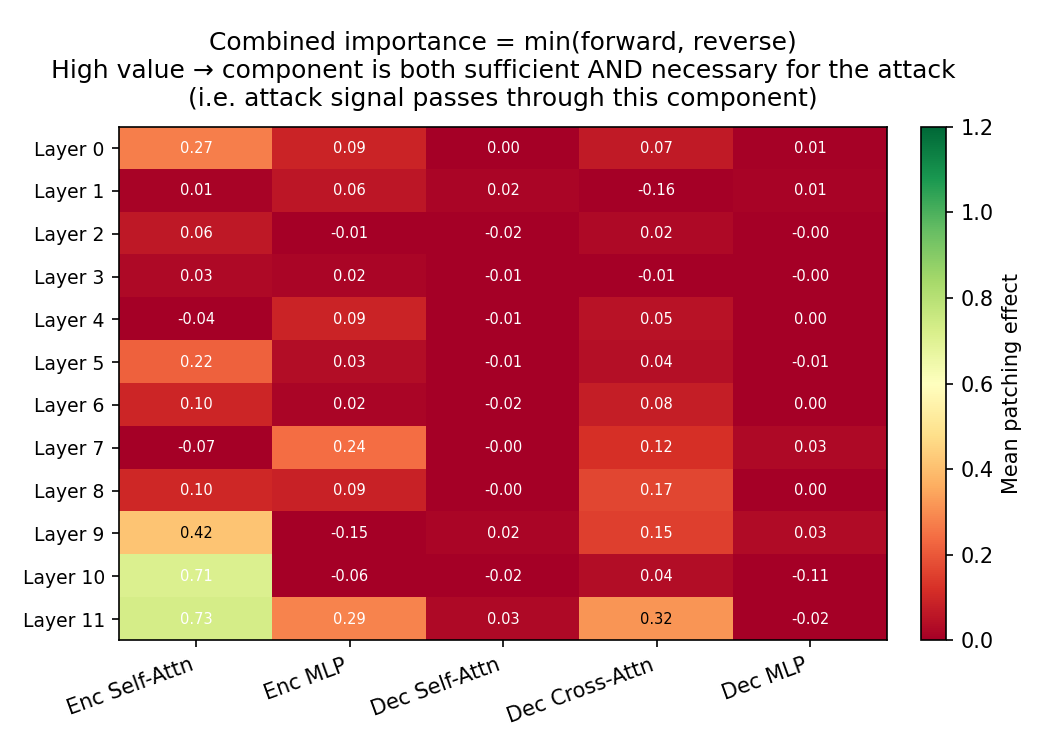
\includegraphics[width=0.17\textwidth]{outputs/attacks/false_end_2/plots/combined_layer_component_heatmap.png} & 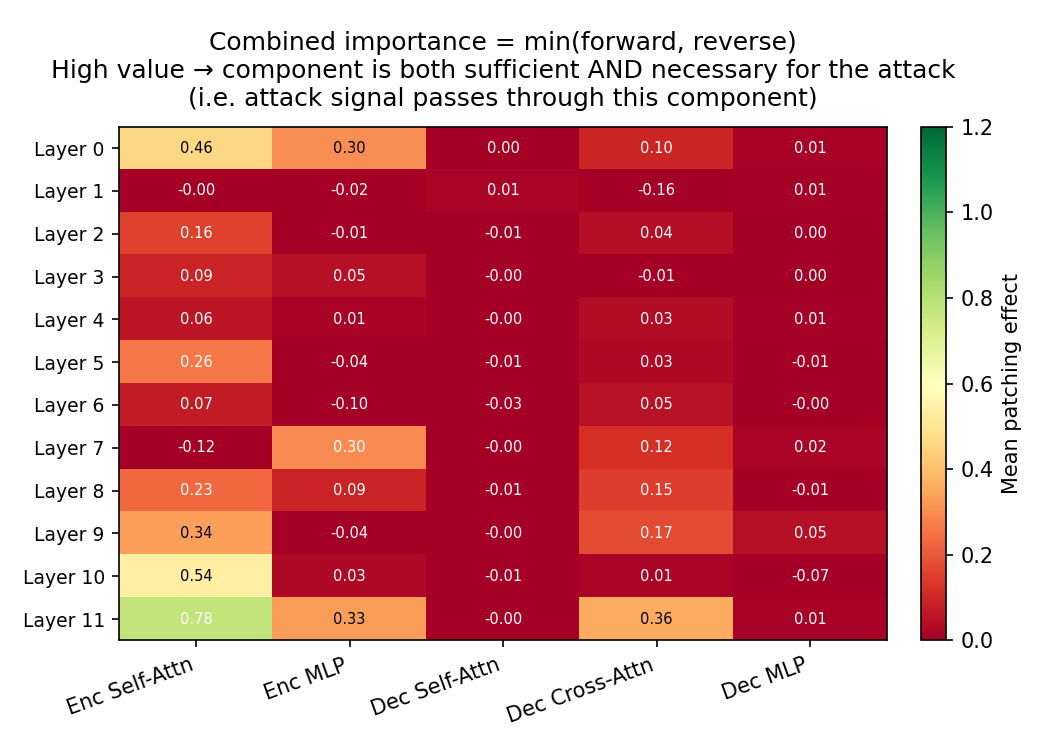
\includegraphics[width=0.17\textwidth]{outputs/attacks/false_end_3/plots/combined_layer_component_heatmap.png} & 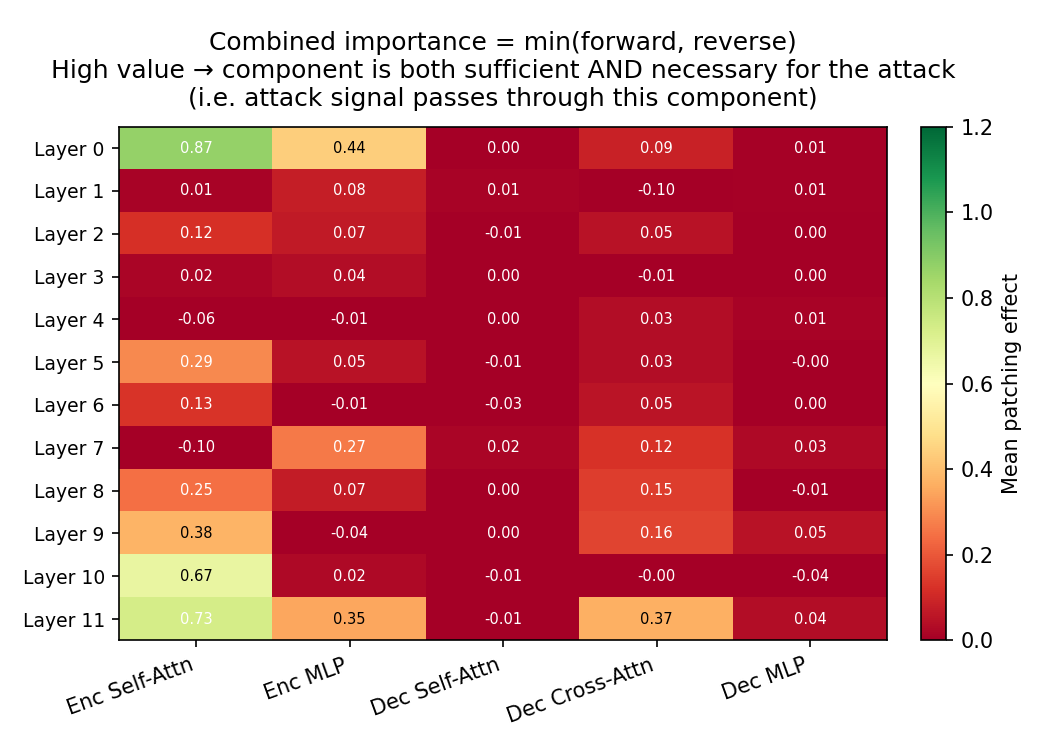
\includegraphics[width=0.17\textwidth]{outputs/attacks/false_end_4/plots/combined_layer_component_heatmap.png} & 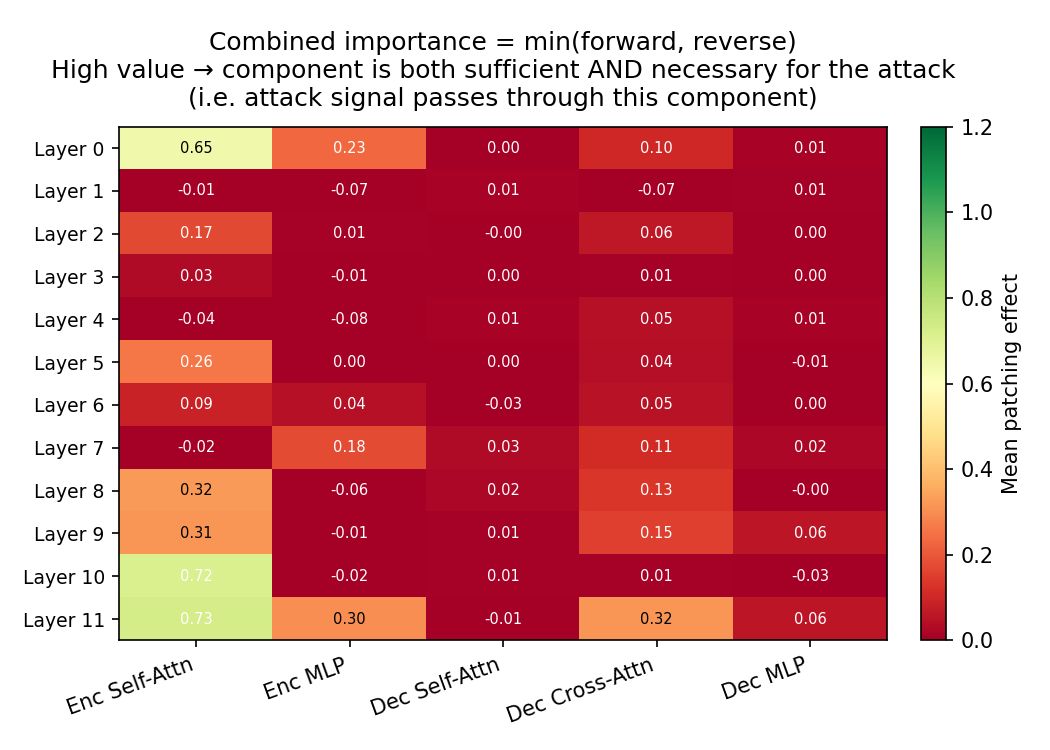
\includegraphics[width=0.17\textwidth]{outputs/attacks/false_end_5/plots/combined_layer_component_heatmap.png} \\[4pt]
\end{tabular}
\caption{Patching heatmaps for \texttt{false_end}: forward (top), reverse (middle), combined (bottom) across repetitions 1--5.}
\label{fig:hm:false_end}
\end{figure}

\begin{figure}[H]
\centering
\setlength{\tabcolsep}{2pt}
\renewcommand{\arraystretch}{0.5}
\begin{tabular}{r ccccc}
& \textbf{rep=1} & \textbf{rep=2} & \textbf{rep=3} & \textbf{rep=4} & \textbf{rep=5} \\[2pt]
\rotatebox{90}{\textbf{forward}} & 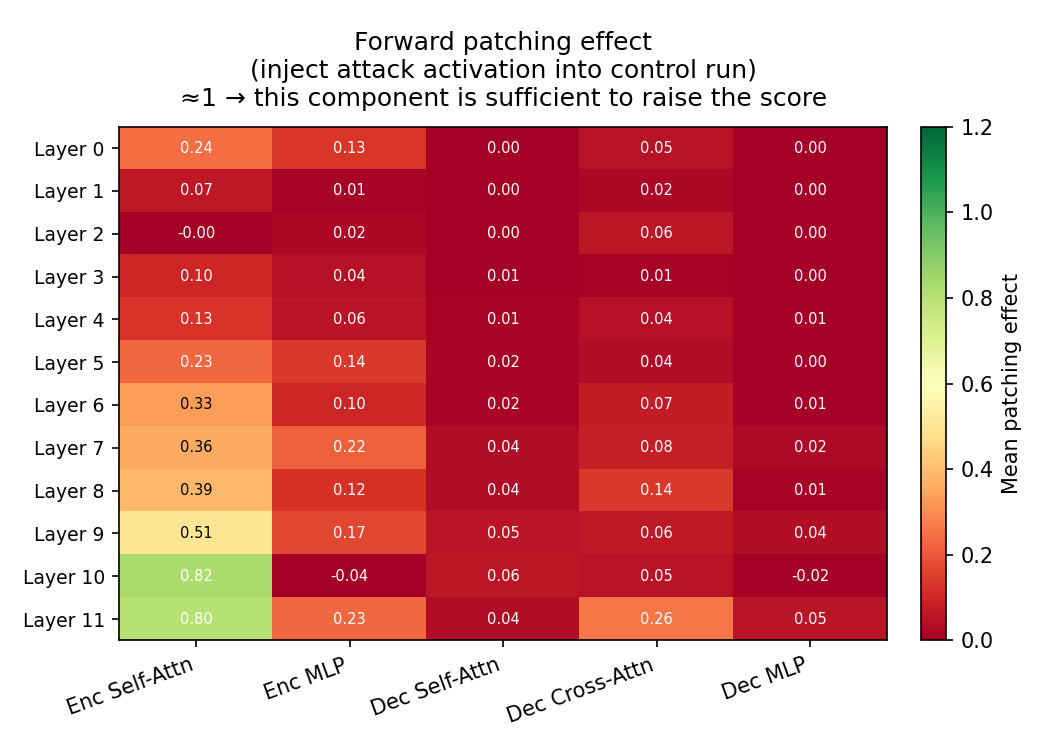
\includegraphics[width=0.17\textwidth]{outputs/attacks/false_random_1/plots/forward_layer_component_heatmap.png} & 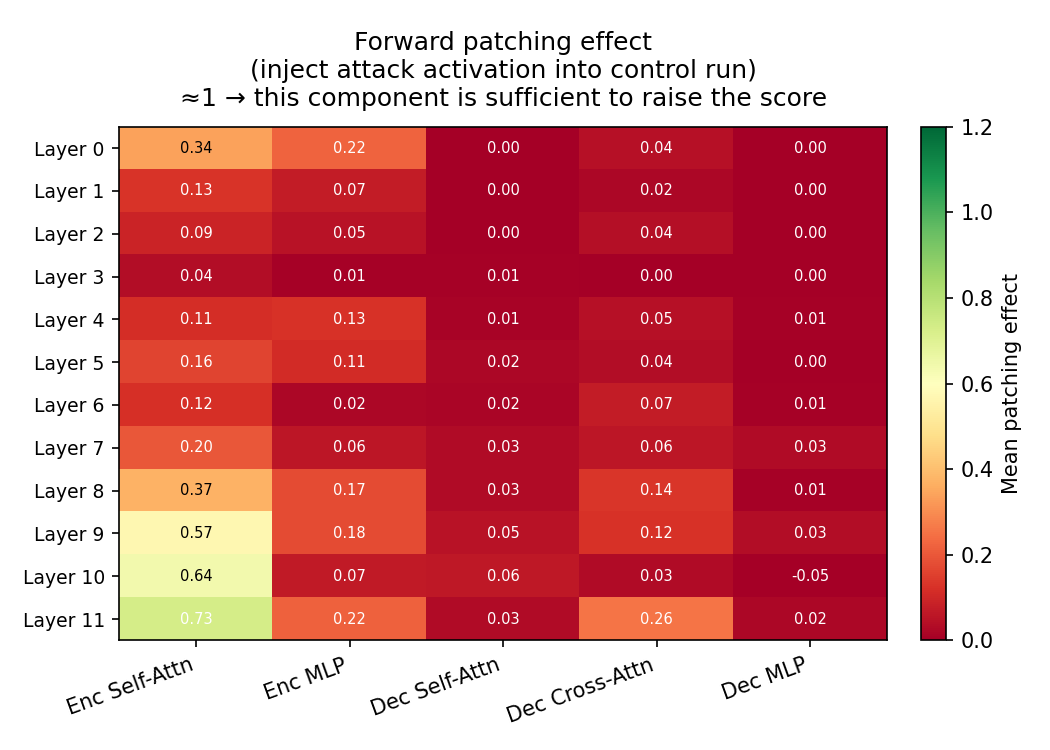
\includegraphics[width=0.17\textwidth]{outputs/attacks/false_random_2/plots/forward_layer_component_heatmap.png} & 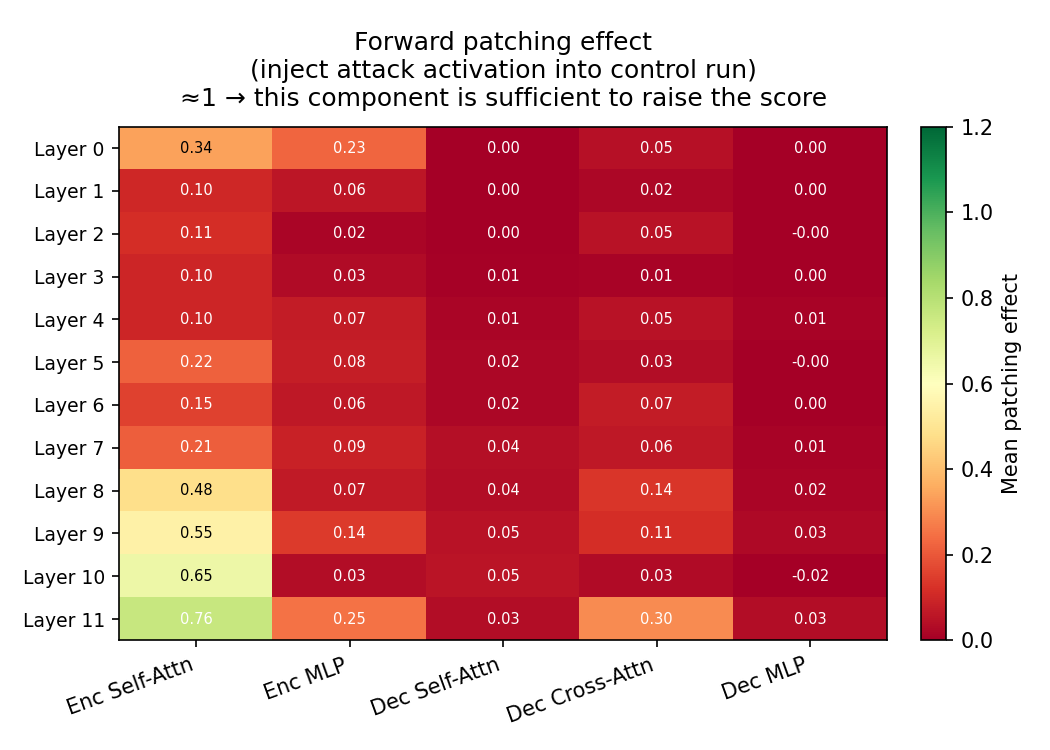
\includegraphics[width=0.17\textwidth]{outputs/attacks/false_random_3/plots/forward_layer_component_heatmap.png} & 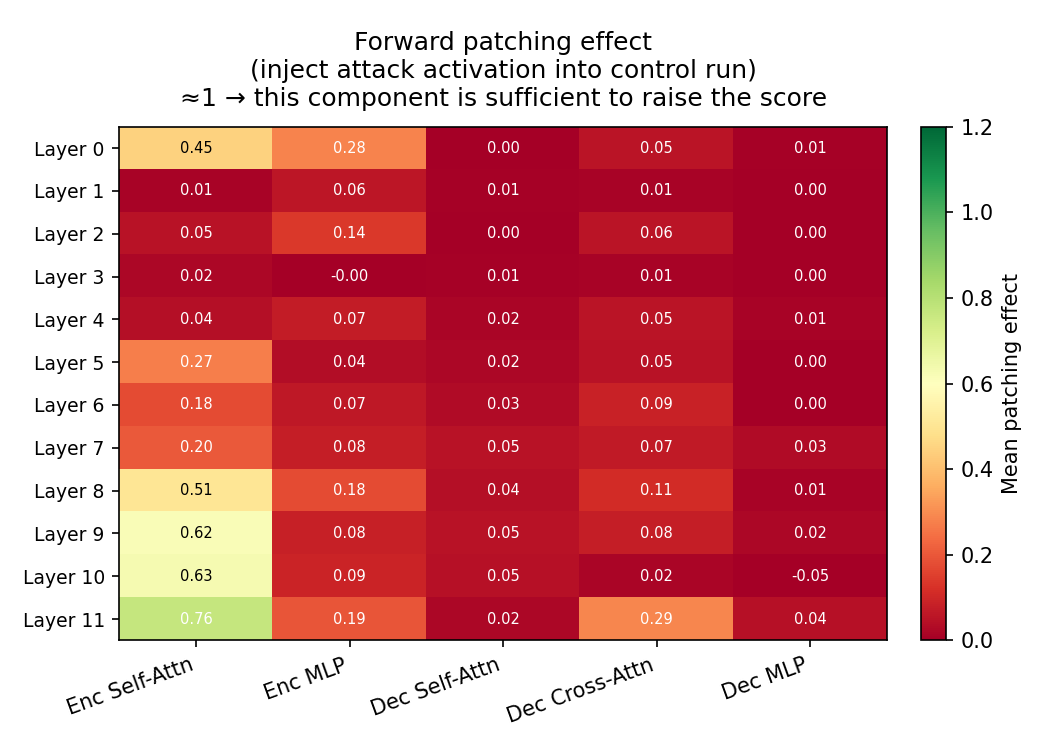
\includegraphics[width=0.17\textwidth]{outputs/attacks/false_random_4/plots/forward_layer_component_heatmap.png} & 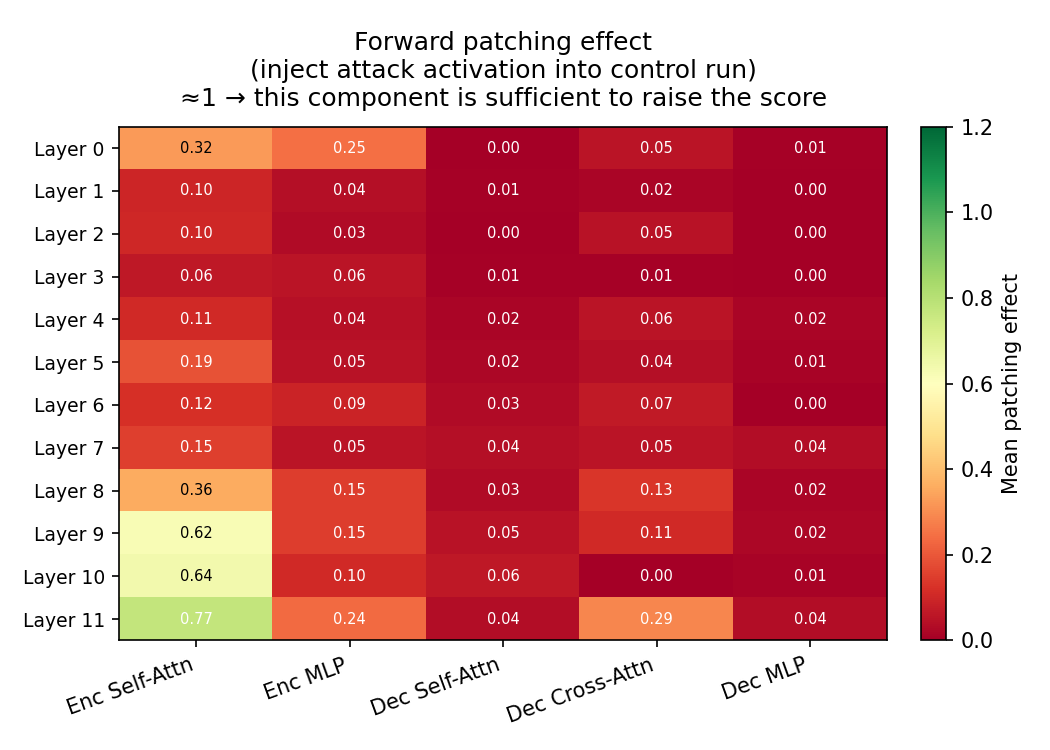
\includegraphics[width=0.17\textwidth]{outputs/attacks/false_random_5/plots/forward_layer_component_heatmap.png} \\[4pt]
\rotatebox{90}{\textbf{reverse}} & 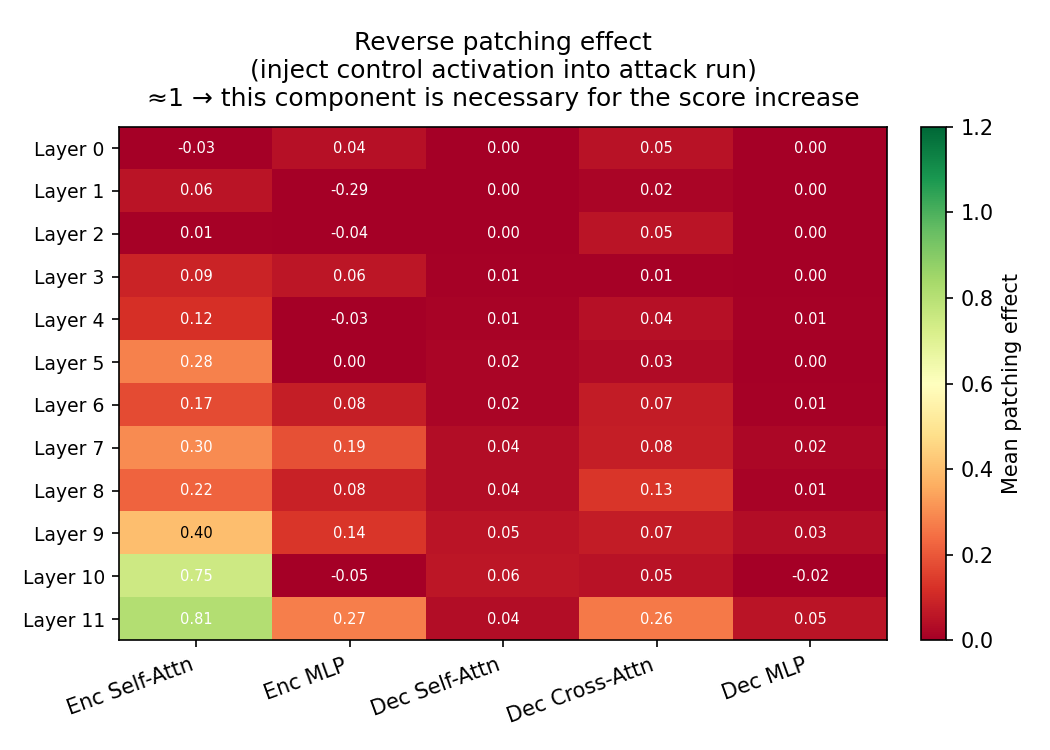
\includegraphics[width=0.17\textwidth]{outputs/attacks/false_random_1/plots/reverse_layer_component_heatmap.png} & 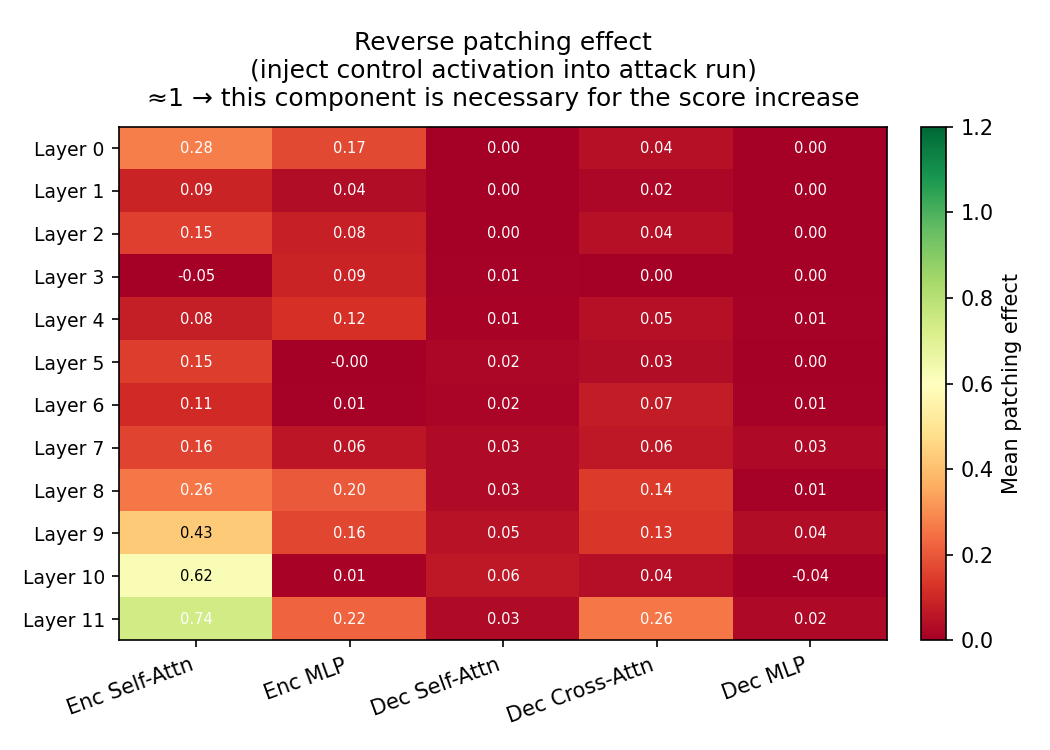
\includegraphics[width=0.17\textwidth]{outputs/attacks/false_random_2/plots/reverse_layer_component_heatmap.png} & 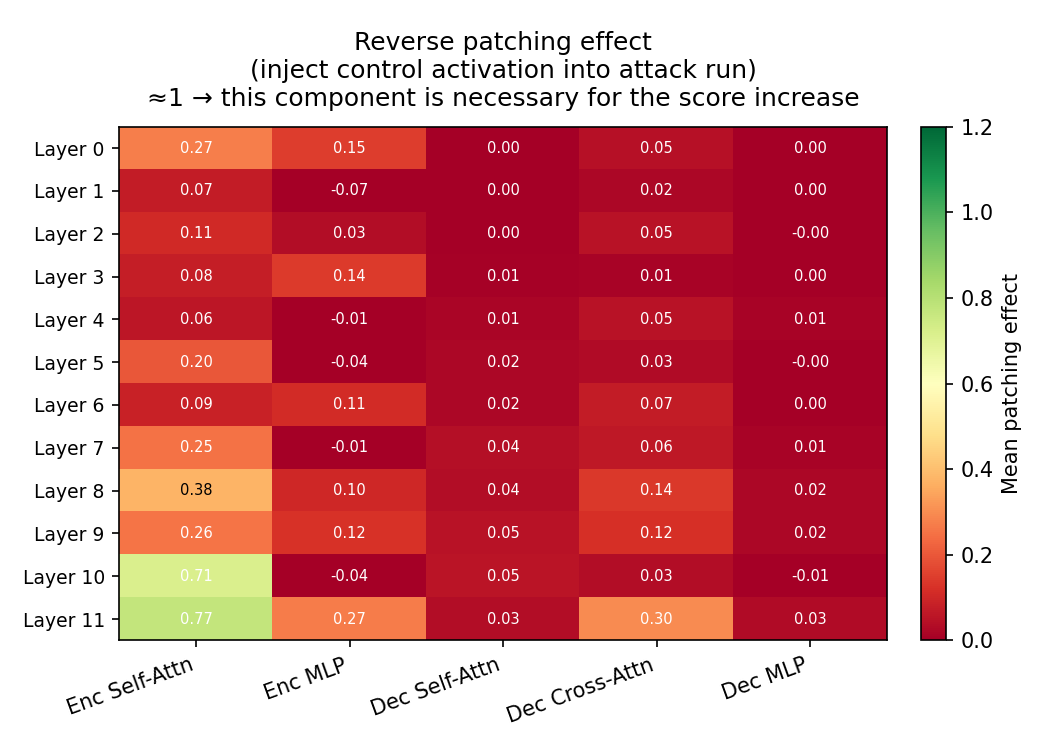
\includegraphics[width=0.17\textwidth]{outputs/attacks/false_random_3/plots/reverse_layer_component_heatmap.png} & 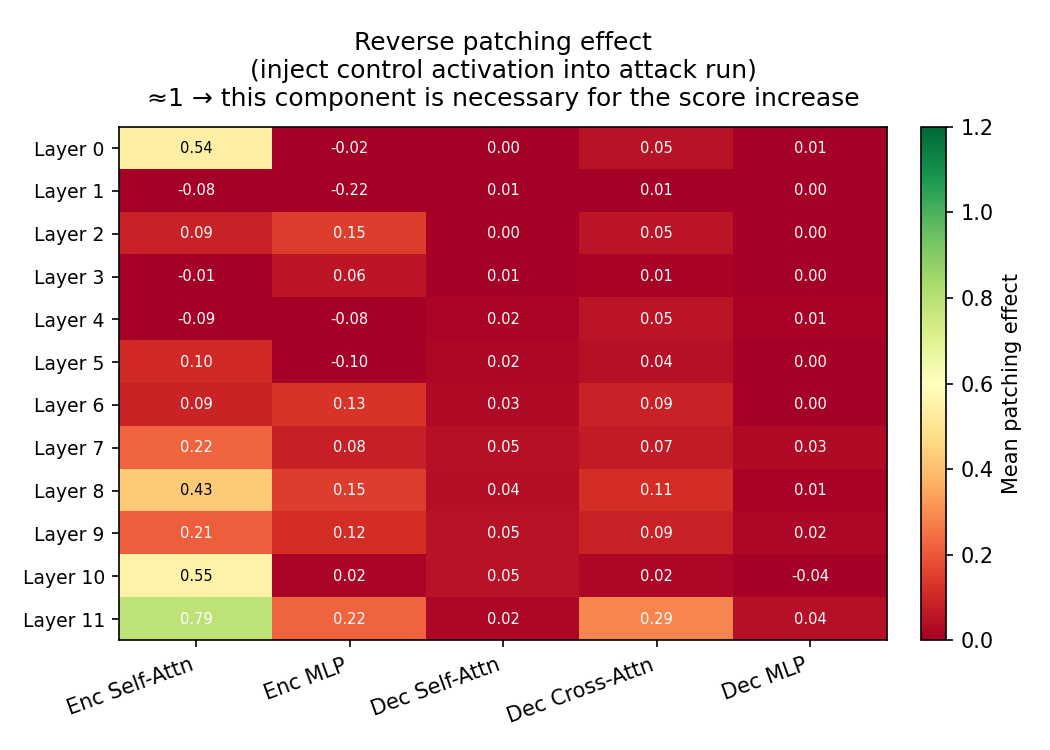
\includegraphics[width=0.17\textwidth]{outputs/attacks/false_random_4/plots/reverse_layer_component_heatmap.png} & 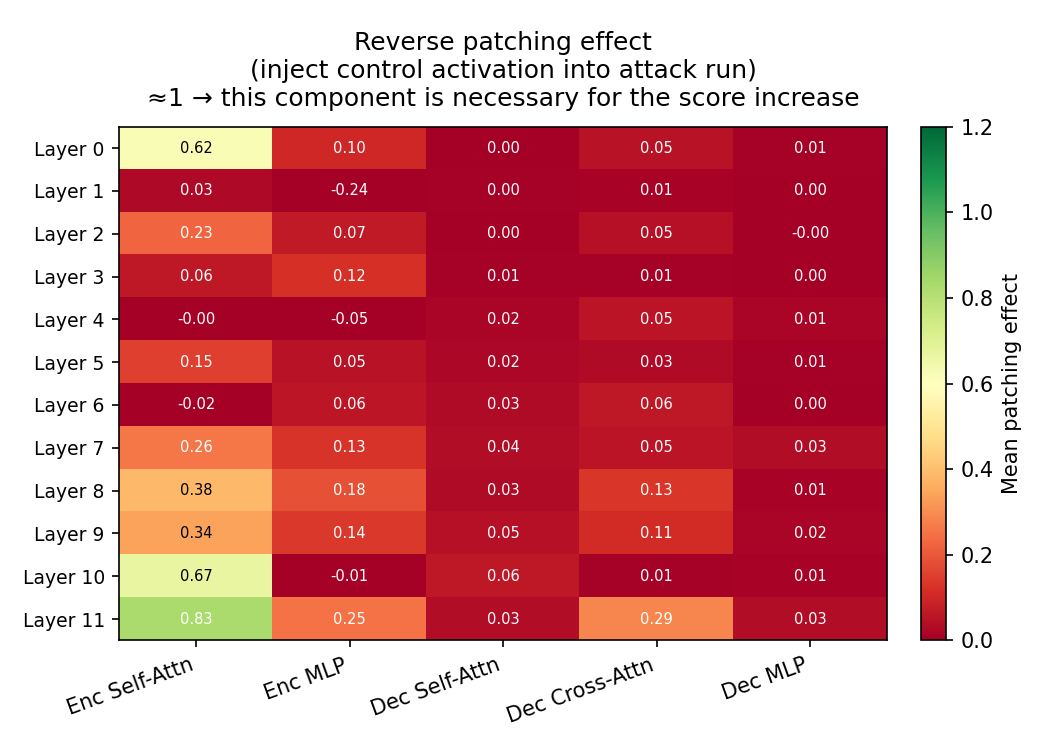
\includegraphics[width=0.17\textwidth]{outputs/attacks/false_random_5/plots/reverse_layer_component_heatmap.png} \\[4pt]
\rotatebox{90}{\textbf{combined}} & 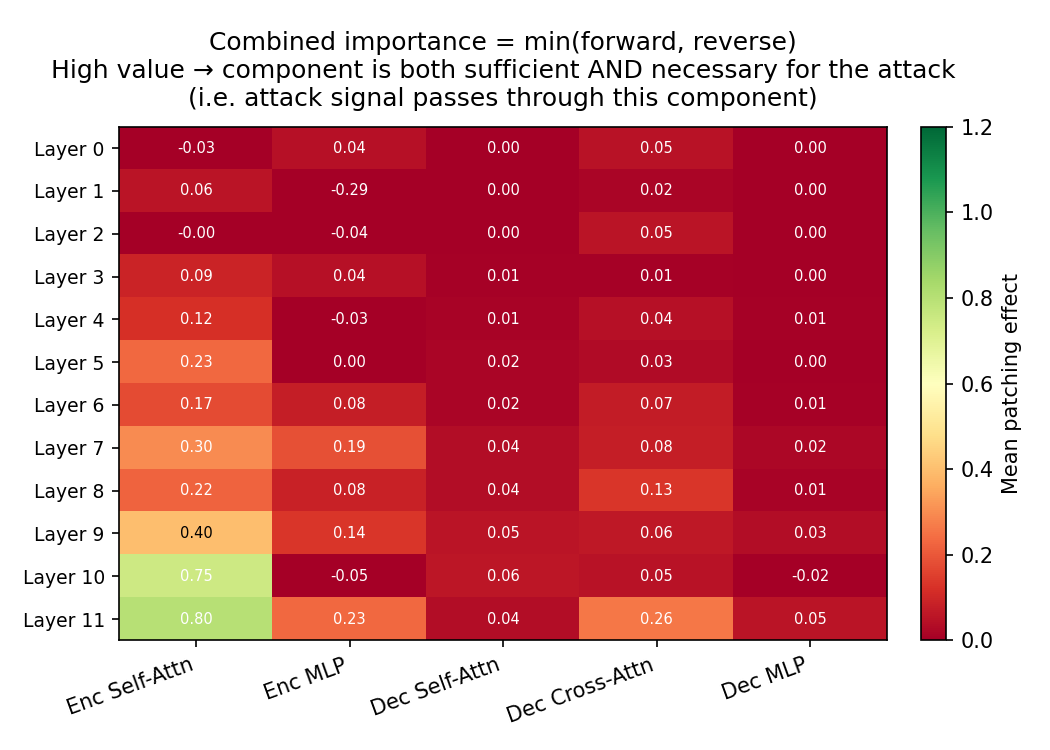
\includegraphics[width=0.17\textwidth]{outputs/attacks/false_random_1/plots/combined_layer_component_heatmap.png} & 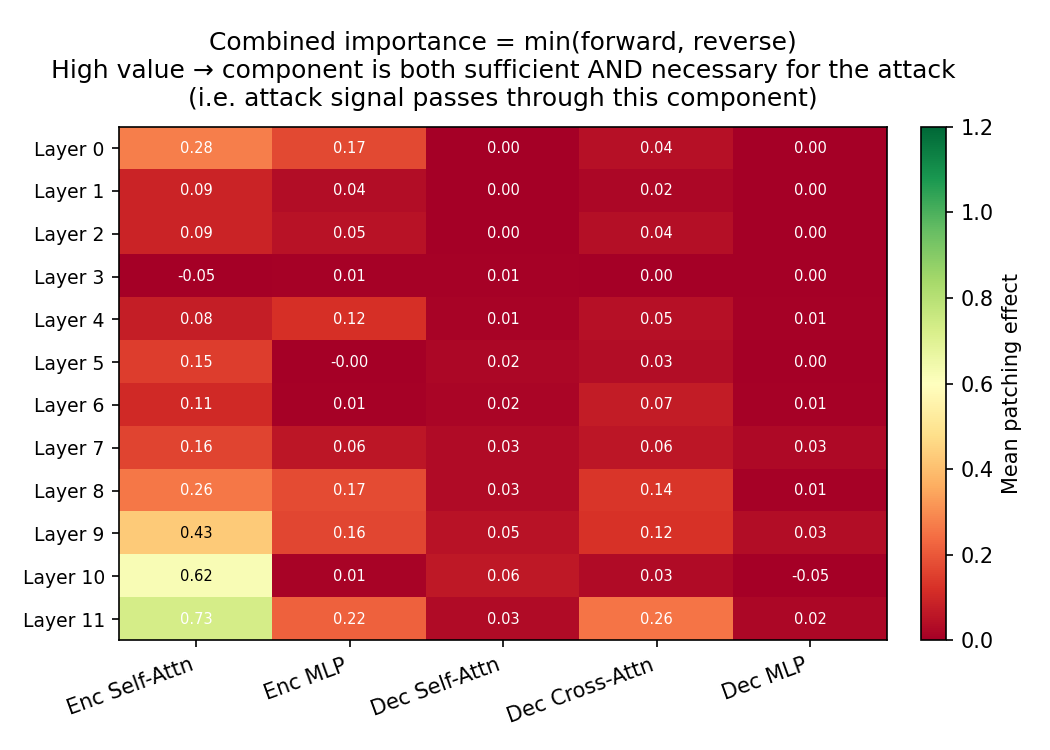
\includegraphics[width=0.17\textwidth]{outputs/attacks/false_random_2/plots/combined_layer_component_heatmap.png} & 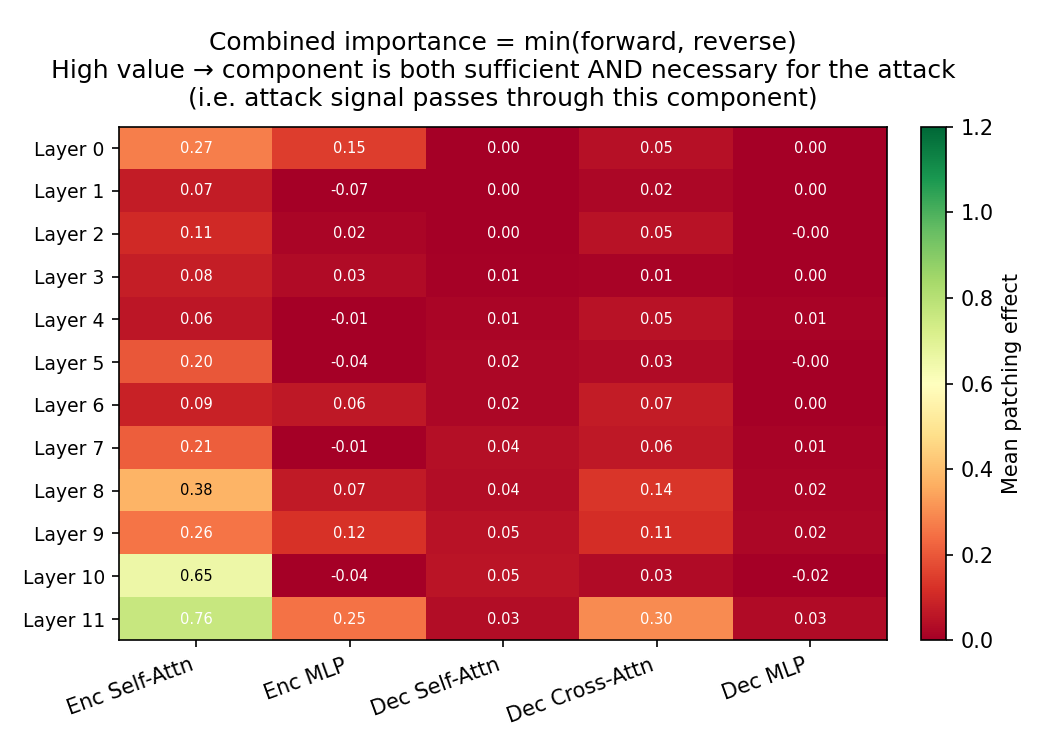
\includegraphics[width=0.17\textwidth]{outputs/attacks/false_random_3/plots/combined_layer_component_heatmap.png} & 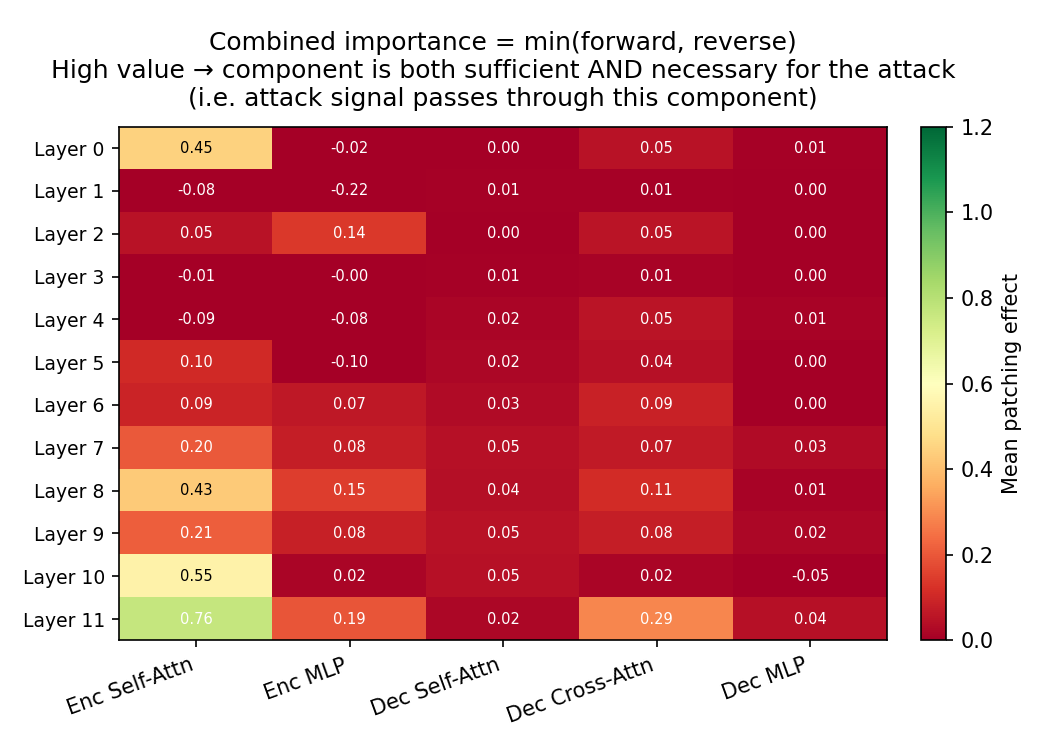
\includegraphics[width=0.17\textwidth]{outputs/attacks/false_random_4/plots/combined_layer_component_heatmap.png} & 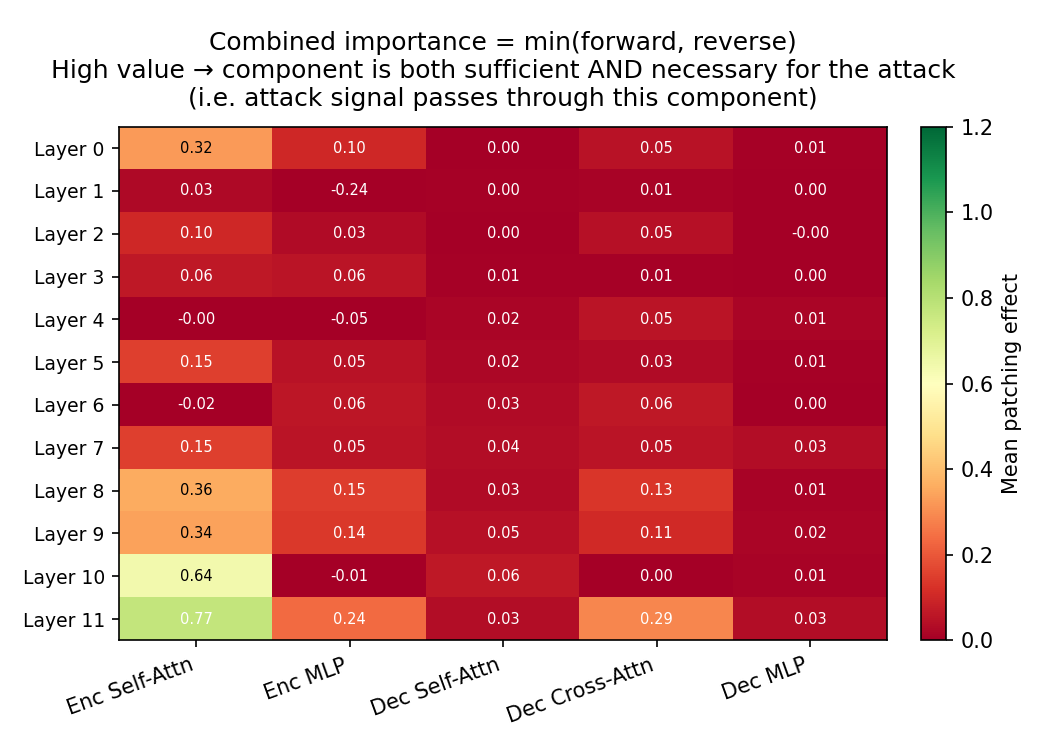
\includegraphics[width=0.17\textwidth]{outputs/attacks/false_random_5/plots/combined_layer_component_heatmap.png} \\[4pt]
\end{tabular}
\caption{Patching heatmaps for \texttt{false_random}: forward (top), reverse (middle), combined (bottom) across repetitions 1--5.}
\label{fig:hm:false_random}
\end{figure}

\begin{figure}[H]
\centering
\setlength{\tabcolsep}{2pt}
\renewcommand{\arraystretch}{0.5}
\begin{tabular}{r ccccc}
& \textbf{rep=1} & \textbf{rep=2} & \textbf{rep=3} & \textbf{rep=4} & \textbf{rep=5} \\[2pt]
\rotatebox{90}{\textbf{forward}} & 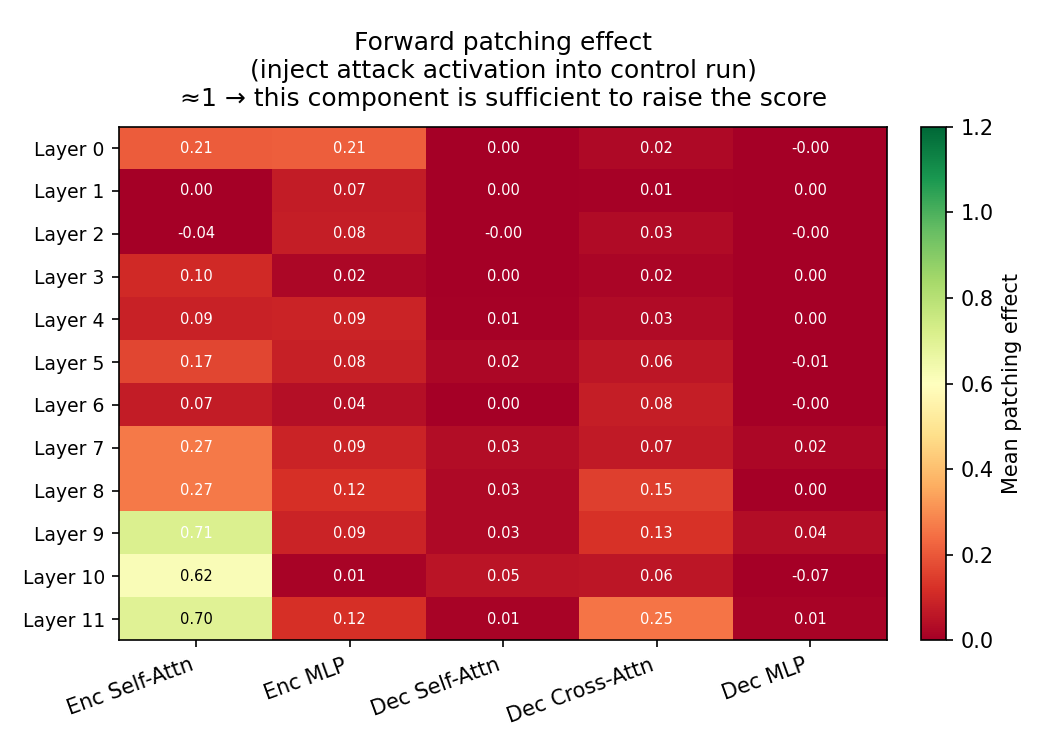
\includegraphics[width=0.17\textwidth]{outputs/attacks/false_start_1/plots/forward_layer_component_heatmap.png} & 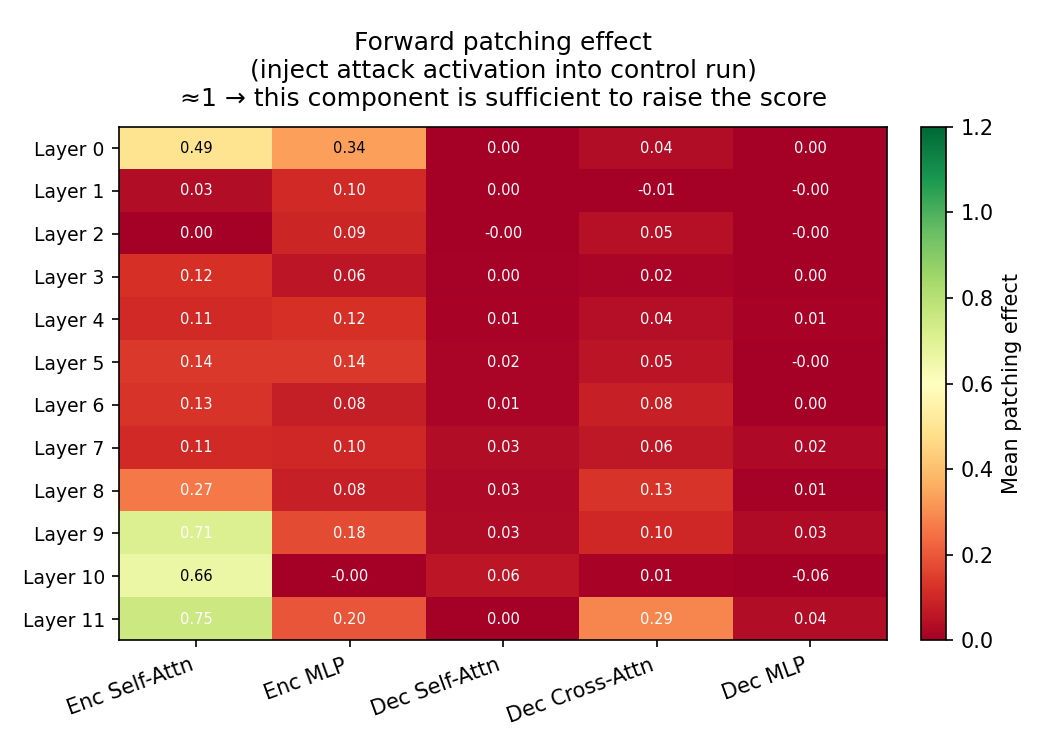
\includegraphics[width=0.17\textwidth]{outputs/attacks/false_start_2/plots/forward_layer_component_heatmap.png} & 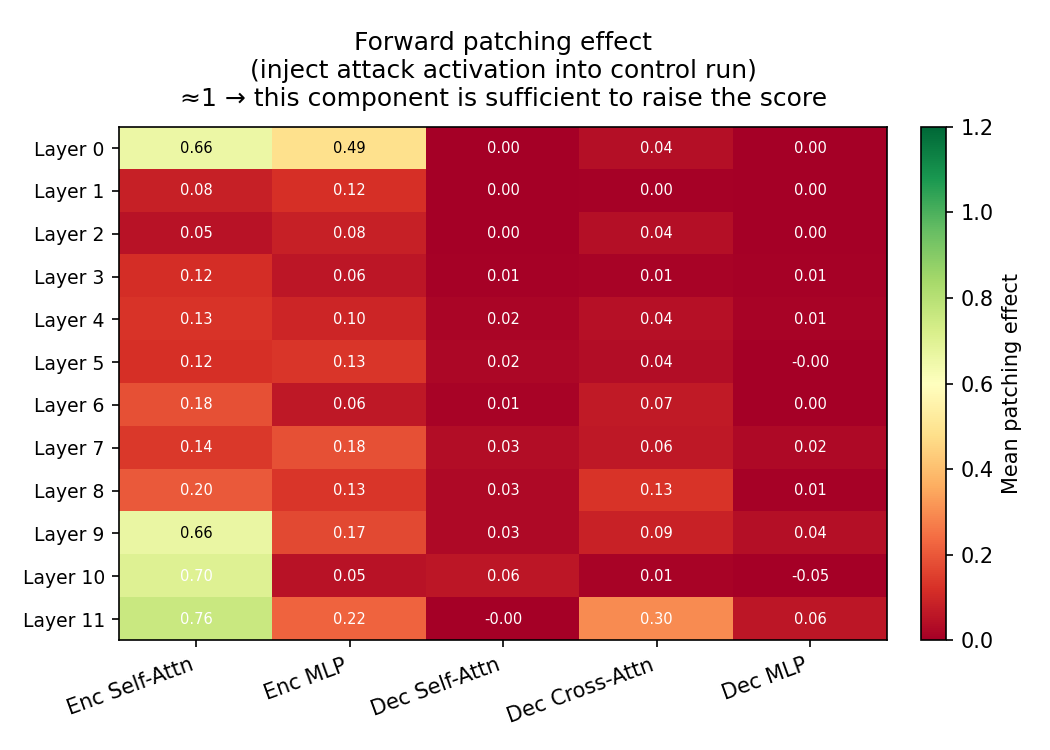
\includegraphics[width=0.17\textwidth]{outputs/attacks/false_start_3/plots/forward_layer_component_heatmap.png} & 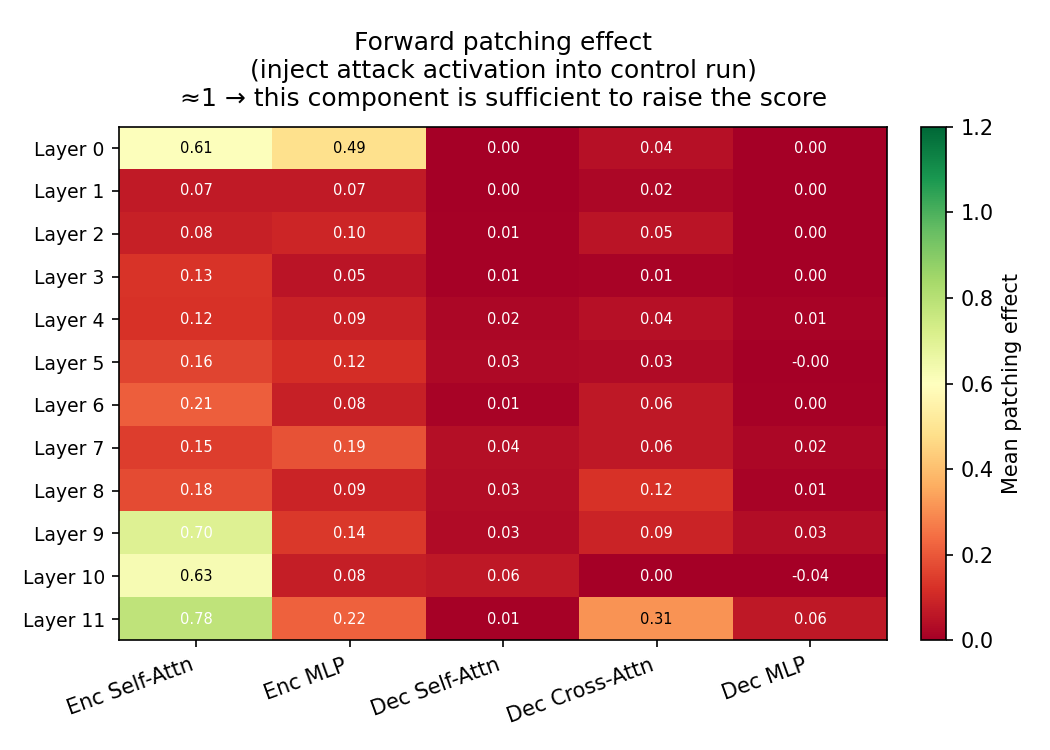
\includegraphics[width=0.17\textwidth]{outputs/attacks/false_start_4/plots/forward_layer_component_heatmap.png} & 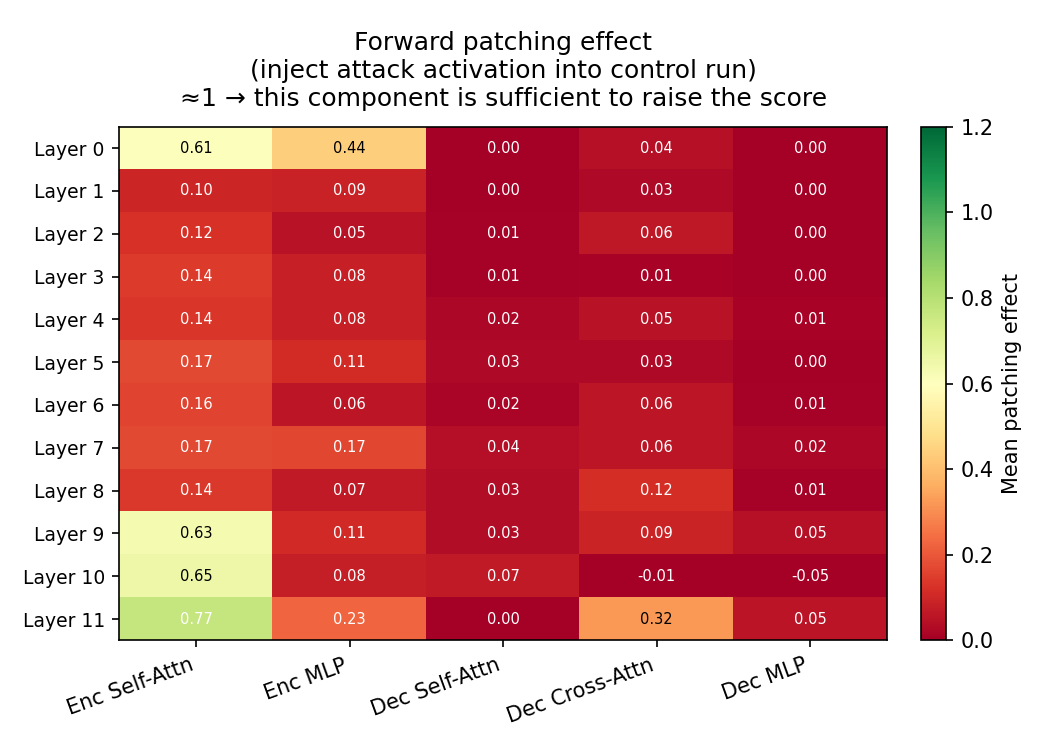
\includegraphics[width=0.17\textwidth]{outputs/attacks/false_start_5/plots/forward_layer_component_heatmap.png} \\[4pt]
\rotatebox{90}{\textbf{reverse}} & 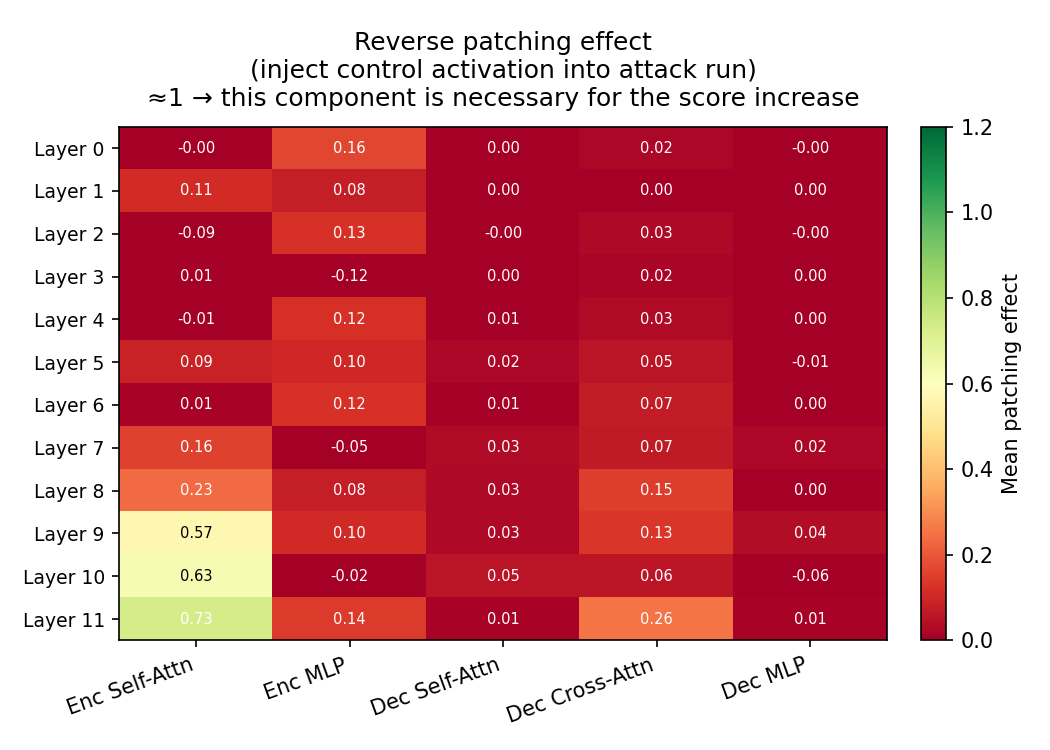
\includegraphics[width=0.17\textwidth]{outputs/attacks/false_start_1/plots/reverse_layer_component_heatmap.png} & 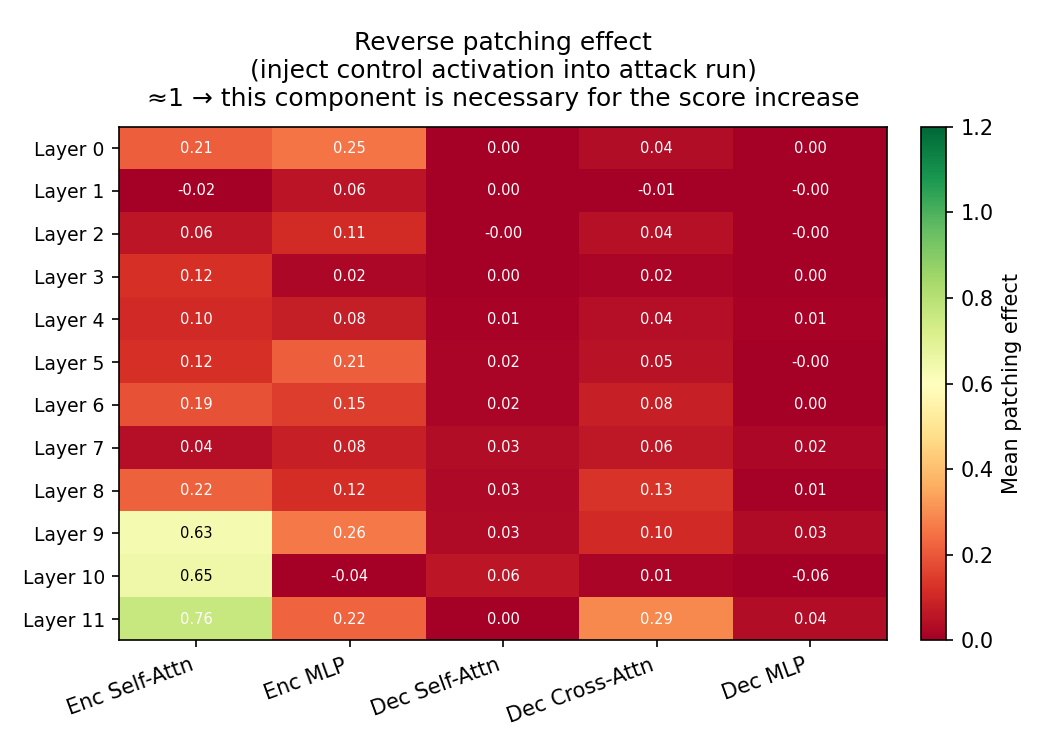
\includegraphics[width=0.17\textwidth]{outputs/attacks/false_start_2/plots/reverse_layer_component_heatmap.png} & 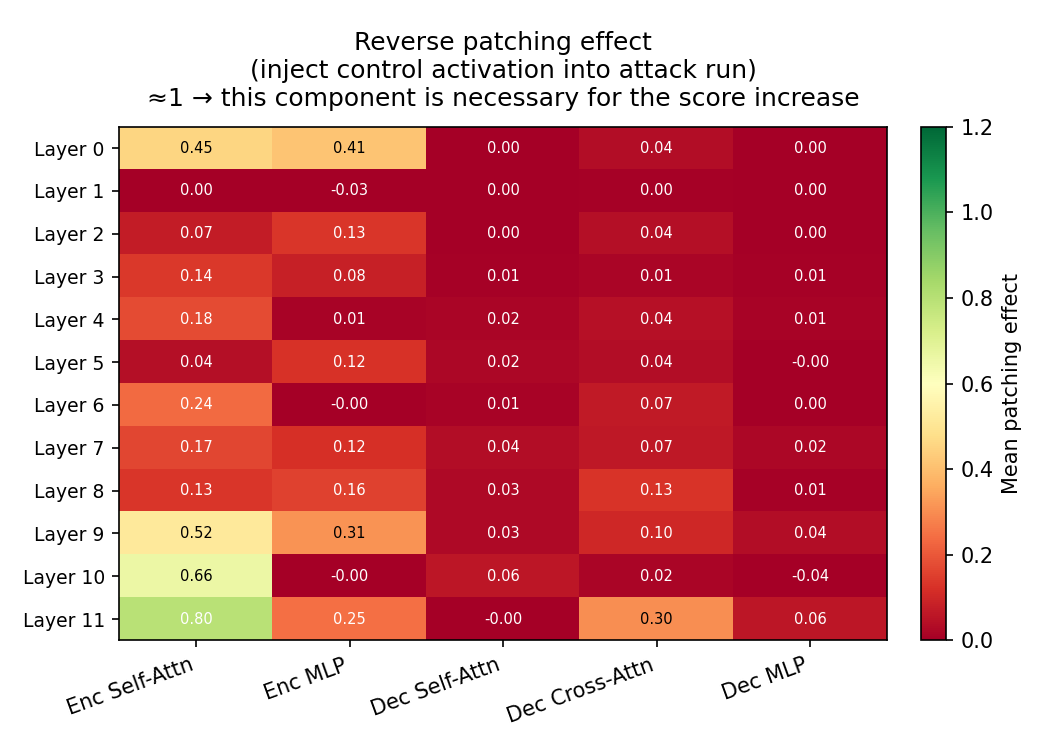
\includegraphics[width=0.17\textwidth]{outputs/attacks/false_start_3/plots/reverse_layer_component_heatmap.png} & 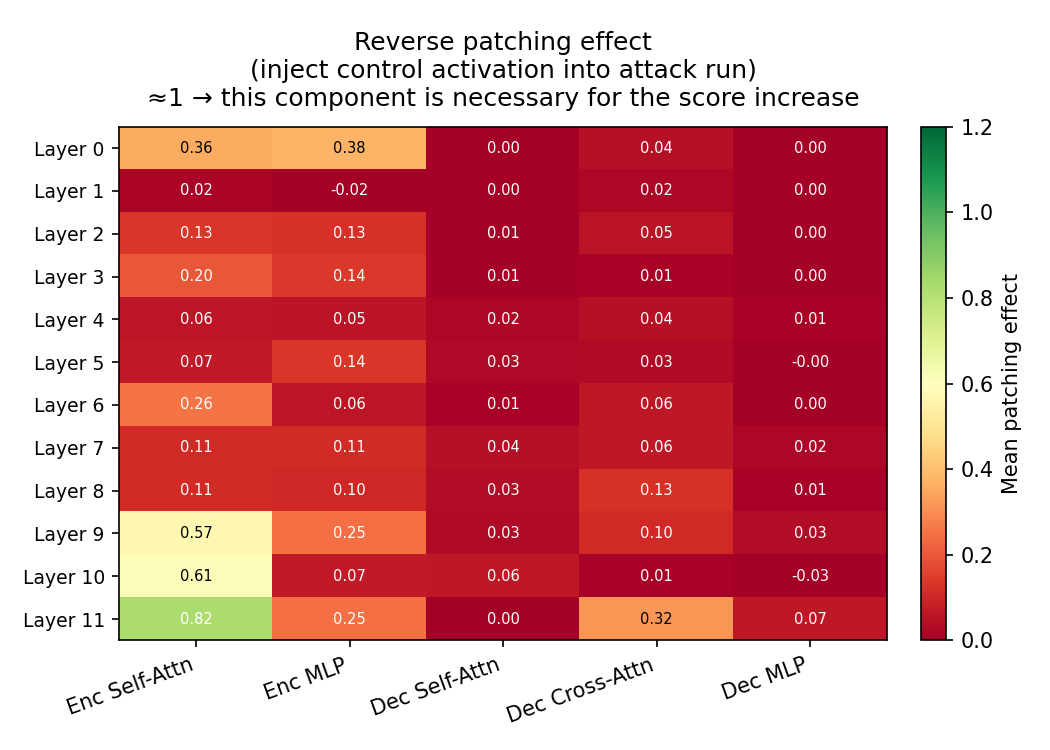
\includegraphics[width=0.17\textwidth]{outputs/attacks/false_start_4/plots/reverse_layer_component_heatmap.png} & 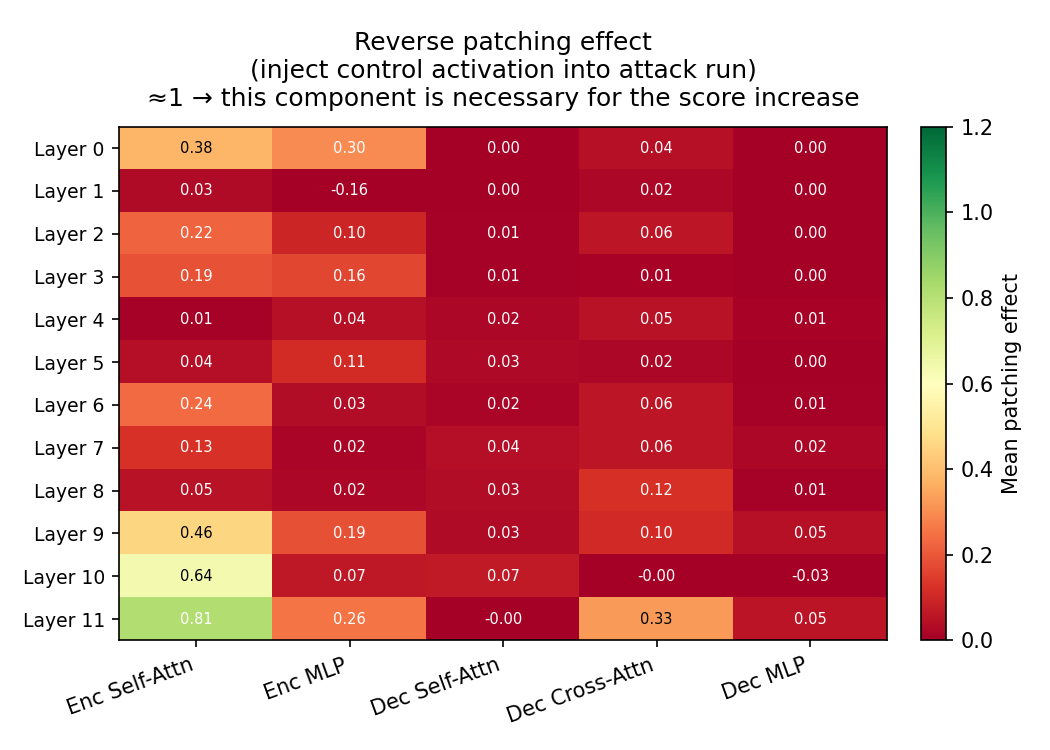
\includegraphics[width=0.17\textwidth]{outputs/attacks/false_start_5/plots/reverse_layer_component_heatmap.png} \\[4pt]
\rotatebox{90}{\textbf{combined}} & 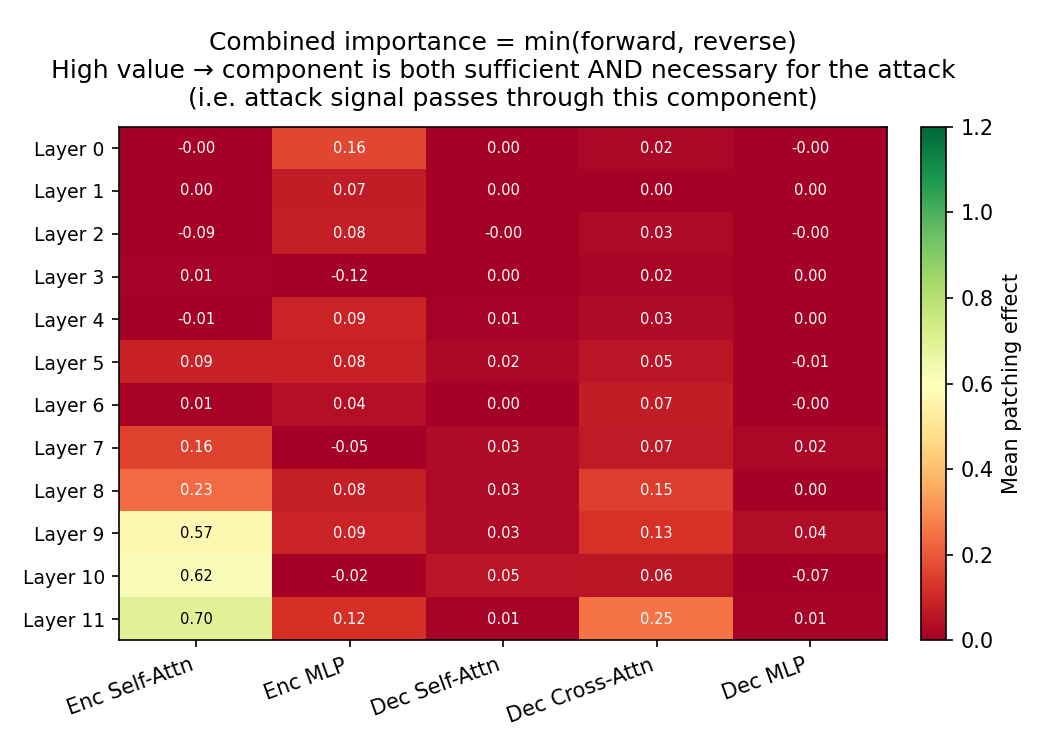
\includegraphics[width=0.17\textwidth]{outputs/attacks/false_start_1/plots/combined_layer_component_heatmap.png} & 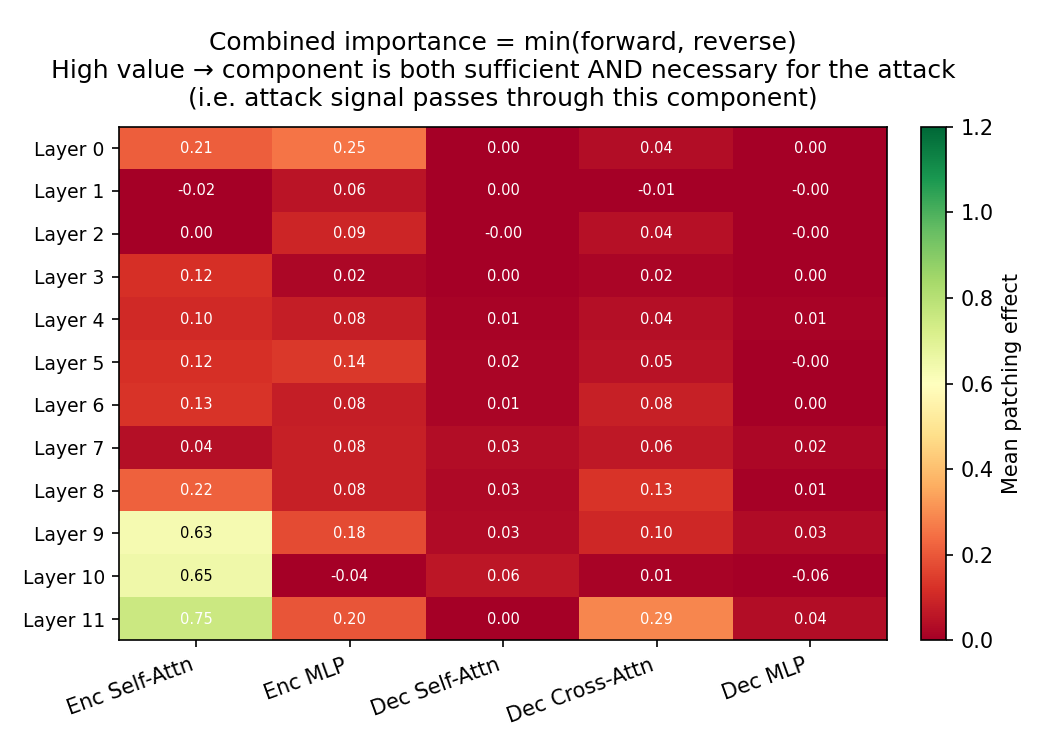
\includegraphics[width=0.17\textwidth]{outputs/attacks/false_start_2/plots/combined_layer_component_heatmap.png} & 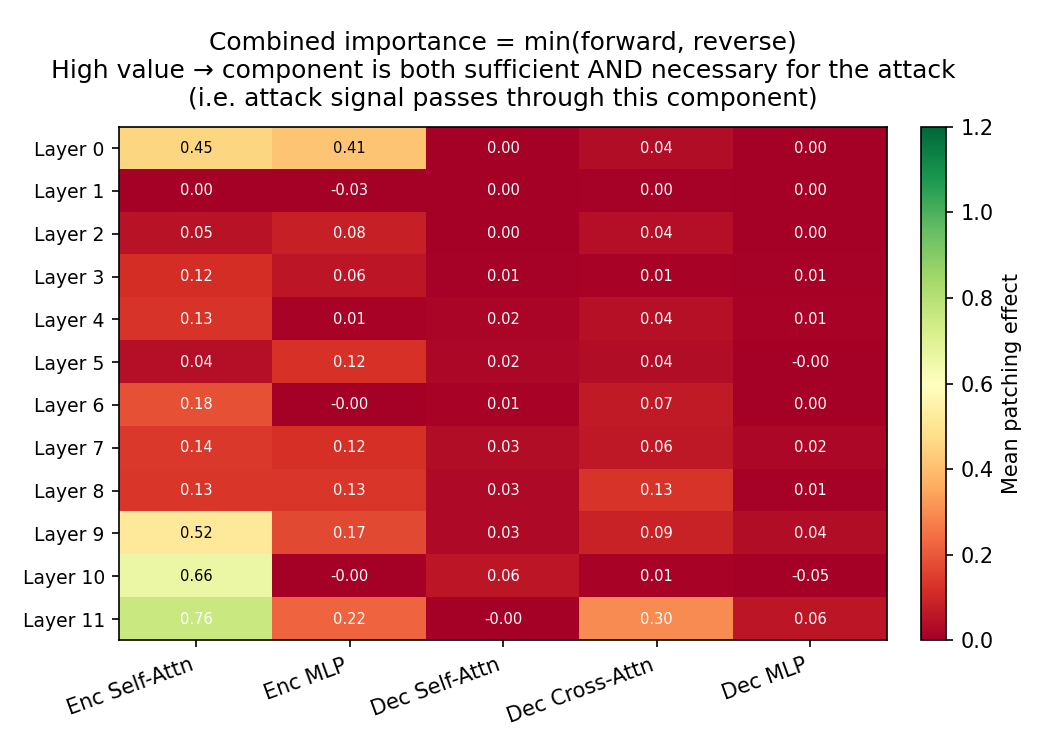
\includegraphics[width=0.17\textwidth]{outputs/attacks/false_start_3/plots/combined_layer_component_heatmap.png} & 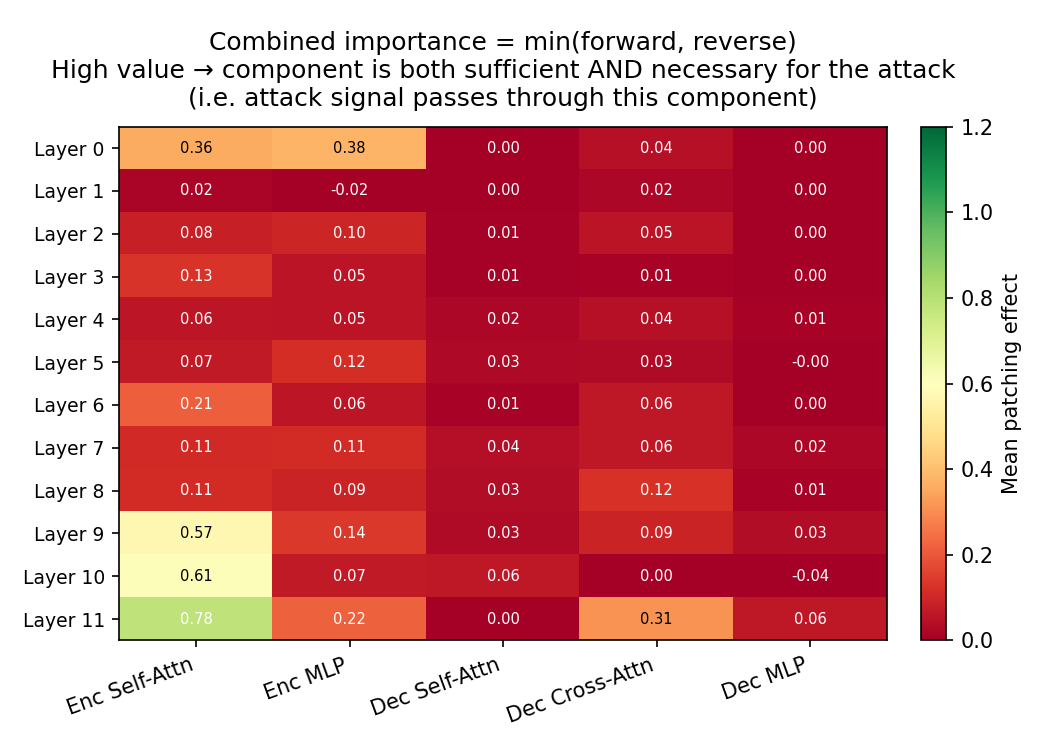
\includegraphics[width=0.17\textwidth]{outputs/attacks/false_start_4/plots/combined_layer_component_heatmap.png} & 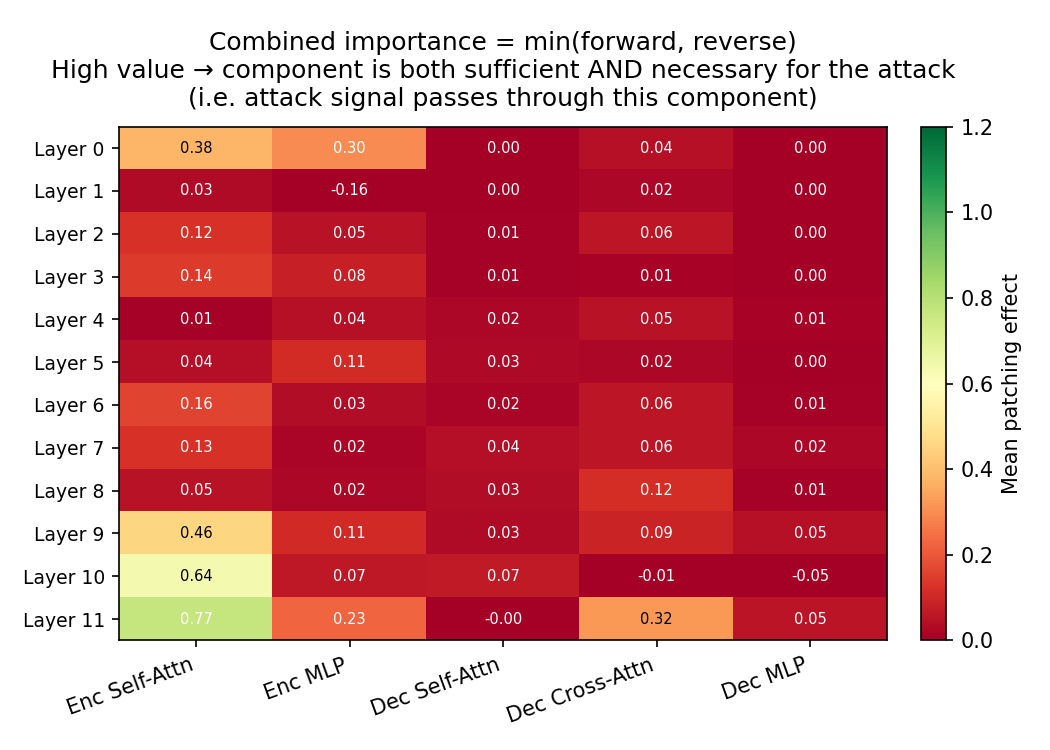
\includegraphics[width=0.17\textwidth]{outputs/attacks/false_start_5/plots/combined_layer_component_heatmap.png} \\[4pt]
\end{tabular}
\caption{Patching heatmaps for \texttt{false_start}: forward (top), reverse (middle), combined (bottom) across repetitions 1--5.}
\label{fig:hm:false_start}
\end{figure}

\begin{figure}[H]
\centering
\setlength{\tabcolsep}{2pt}
\renewcommand{\arraystretch}{0.5}
\begin{tabular}{r ccccc}
& \textbf{rep=1} & \textbf{rep=2} & \textbf{rep=3} & \textbf{rep=4} & \textbf{rep=5} \\[2pt]
\rotatebox{90}{\textbf{forward}} & 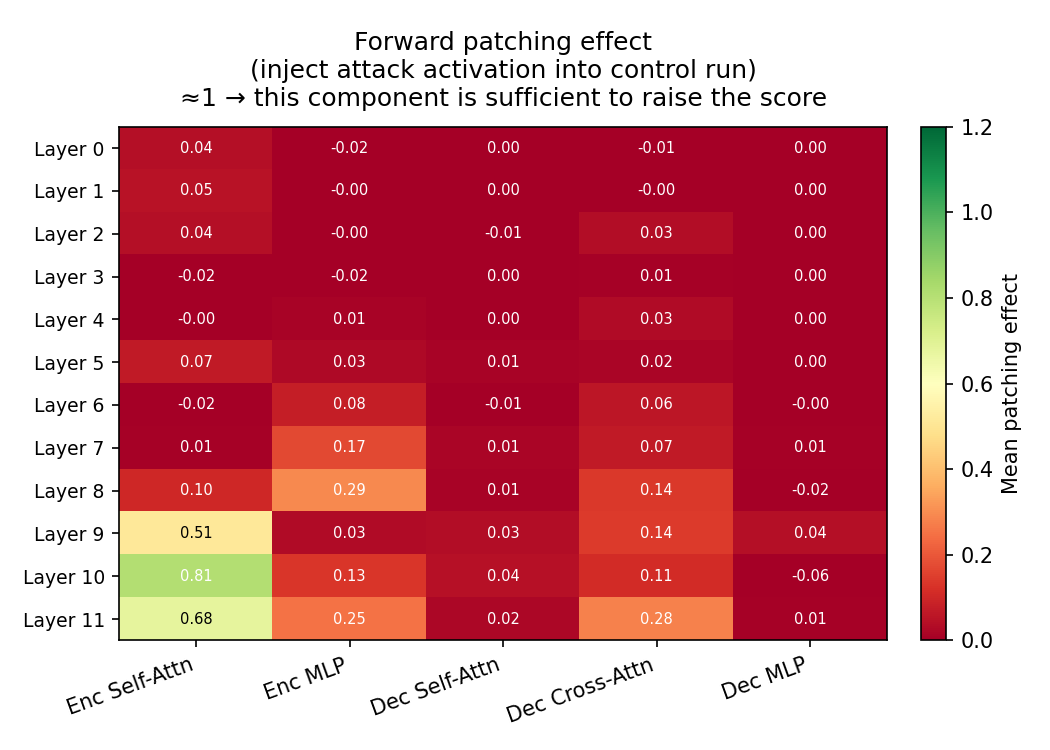
\includegraphics[width=0.17\textwidth]{outputs/attacks/important_end_1/plots/forward_layer_component_heatmap.png} & 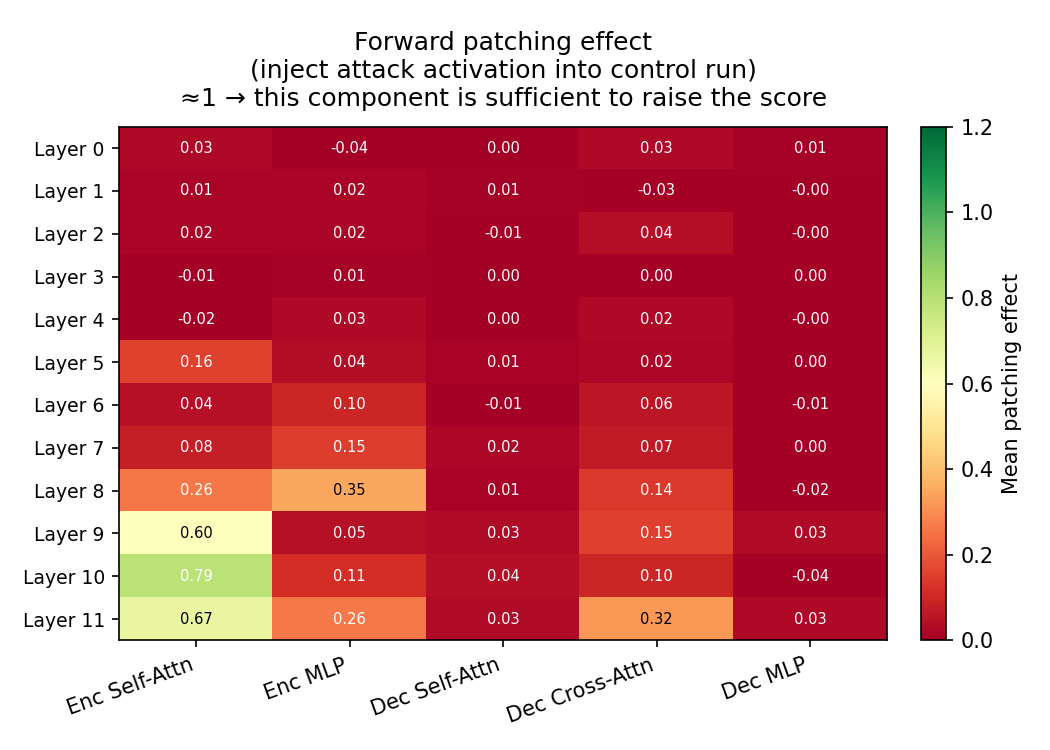
\includegraphics[width=0.17\textwidth]{outputs/attacks/important_end_2/plots/forward_layer_component_heatmap.png} & 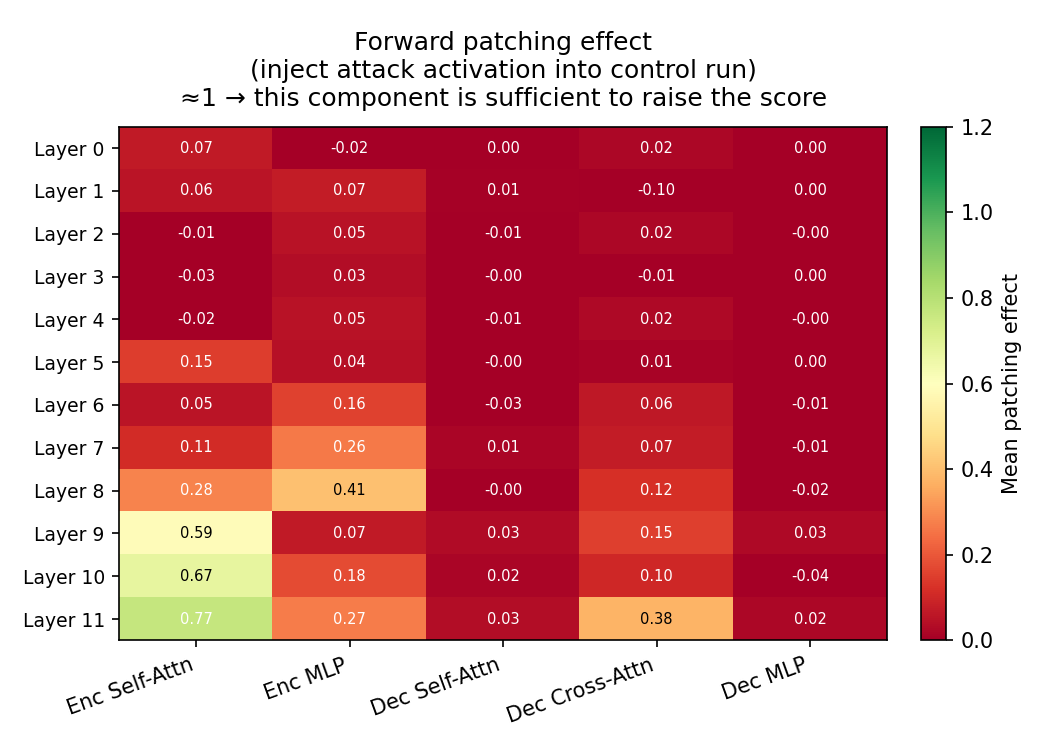
\includegraphics[width=0.17\textwidth]{outputs/attacks/important_end_3/plots/forward_layer_component_heatmap.png} & 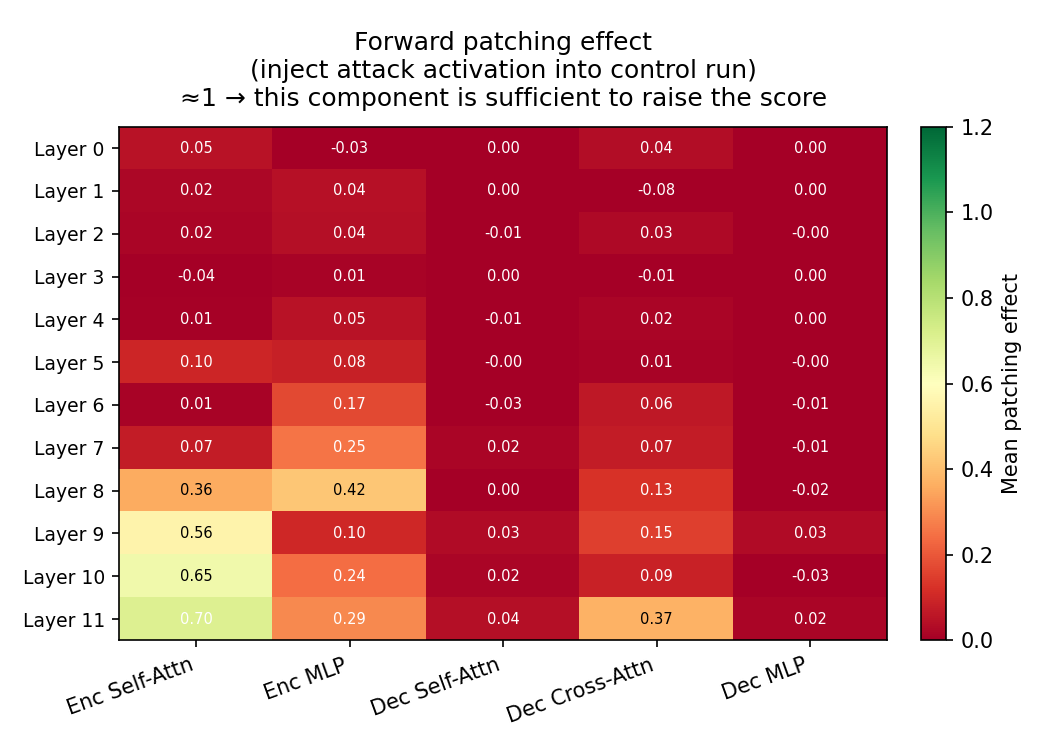
\includegraphics[width=0.17\textwidth]{outputs/attacks/important_end_4/plots/forward_layer_component_heatmap.png} & 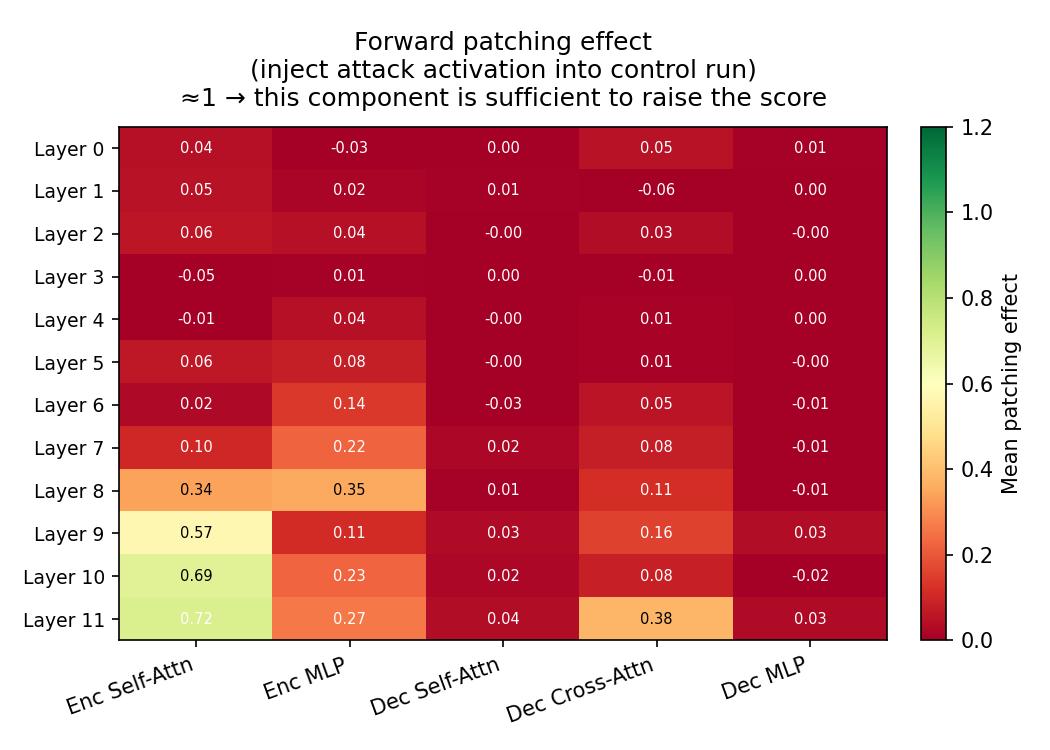
\includegraphics[width=0.17\textwidth]{outputs/attacks/important_end_5/plots/forward_layer_component_heatmap.png} \\[4pt]
\rotatebox{90}{\textbf{reverse}} & 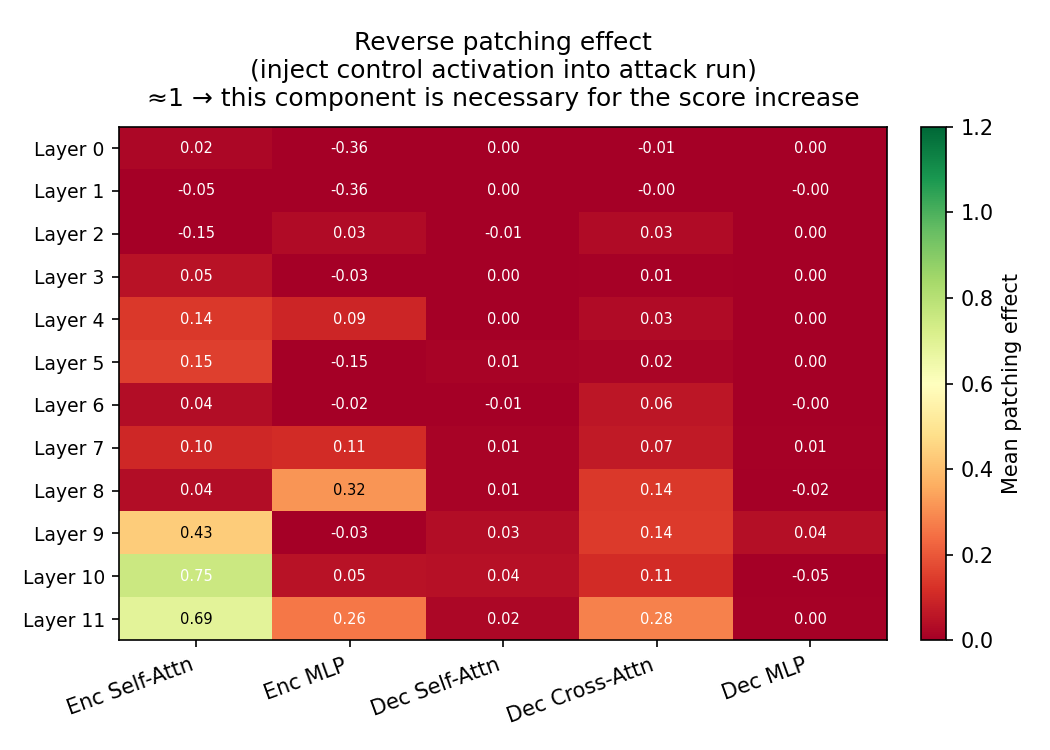
\includegraphics[width=0.17\textwidth]{outputs/attacks/important_end_1/plots/reverse_layer_component_heatmap.png} & 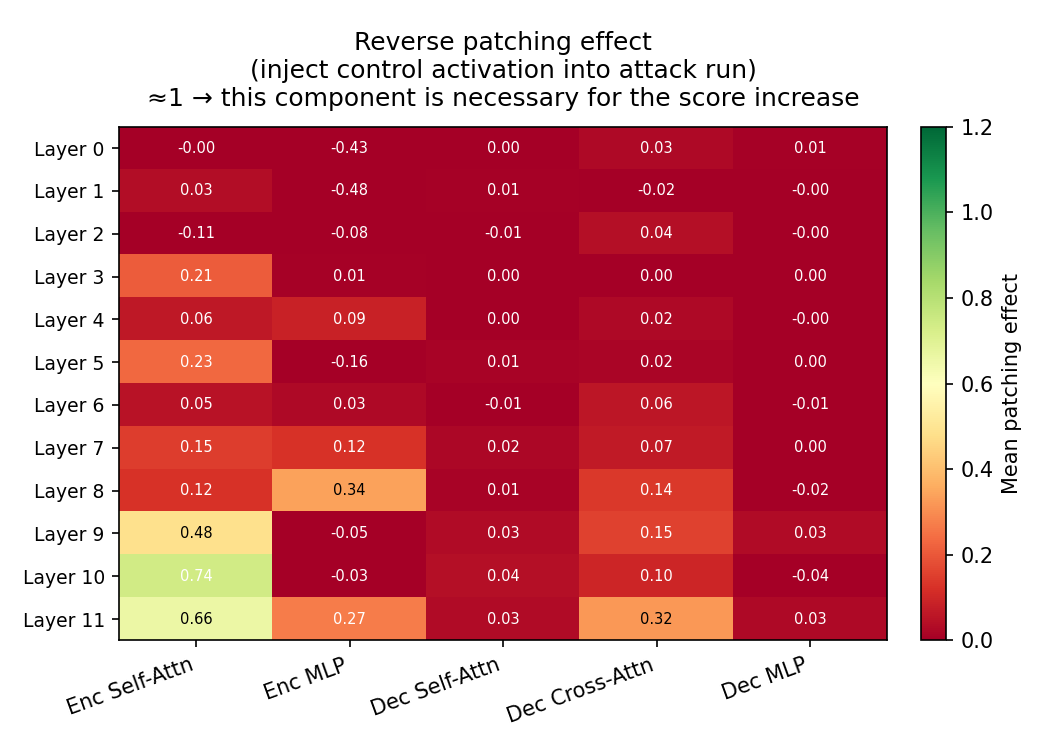
\includegraphics[width=0.17\textwidth]{outputs/attacks/important_end_2/plots/reverse_layer_component_heatmap.png} & 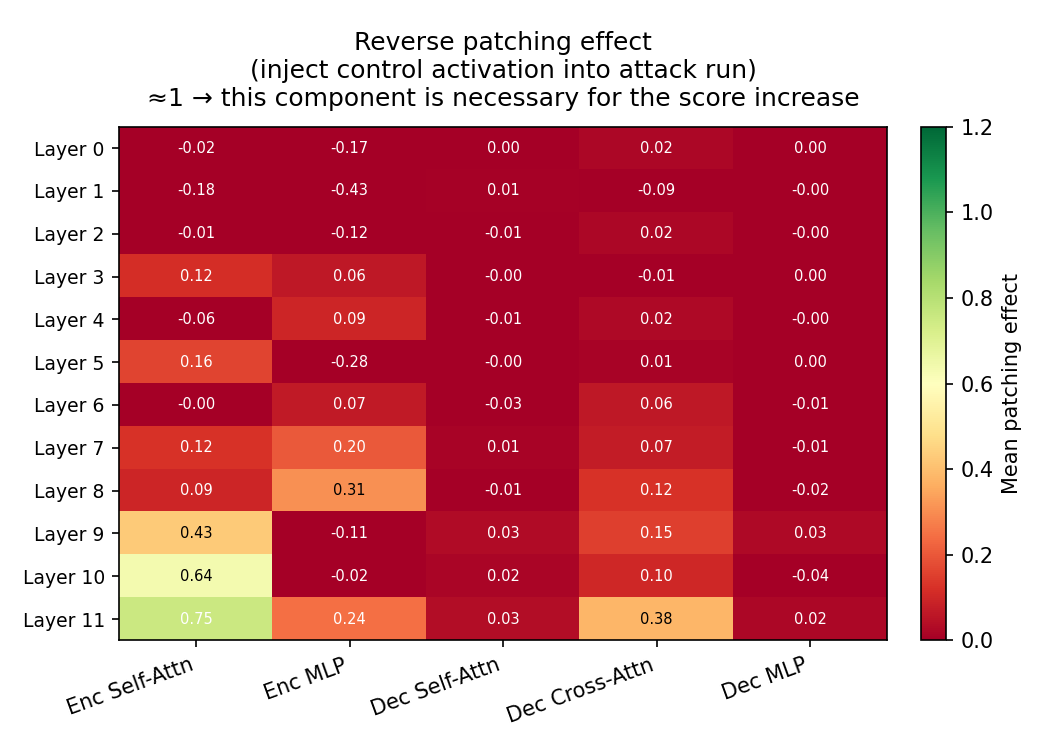
\includegraphics[width=0.17\textwidth]{outputs/attacks/important_end_3/plots/reverse_layer_component_heatmap.png} & 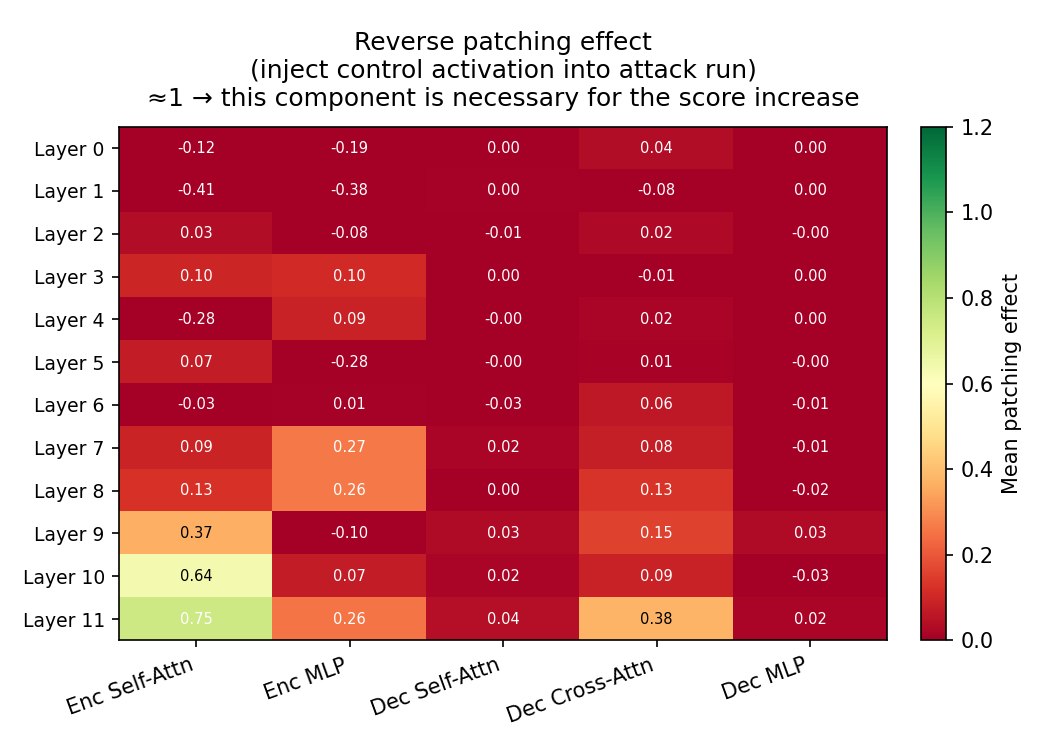
\includegraphics[width=0.17\textwidth]{outputs/attacks/important_end_4/plots/reverse_layer_component_heatmap.png} & 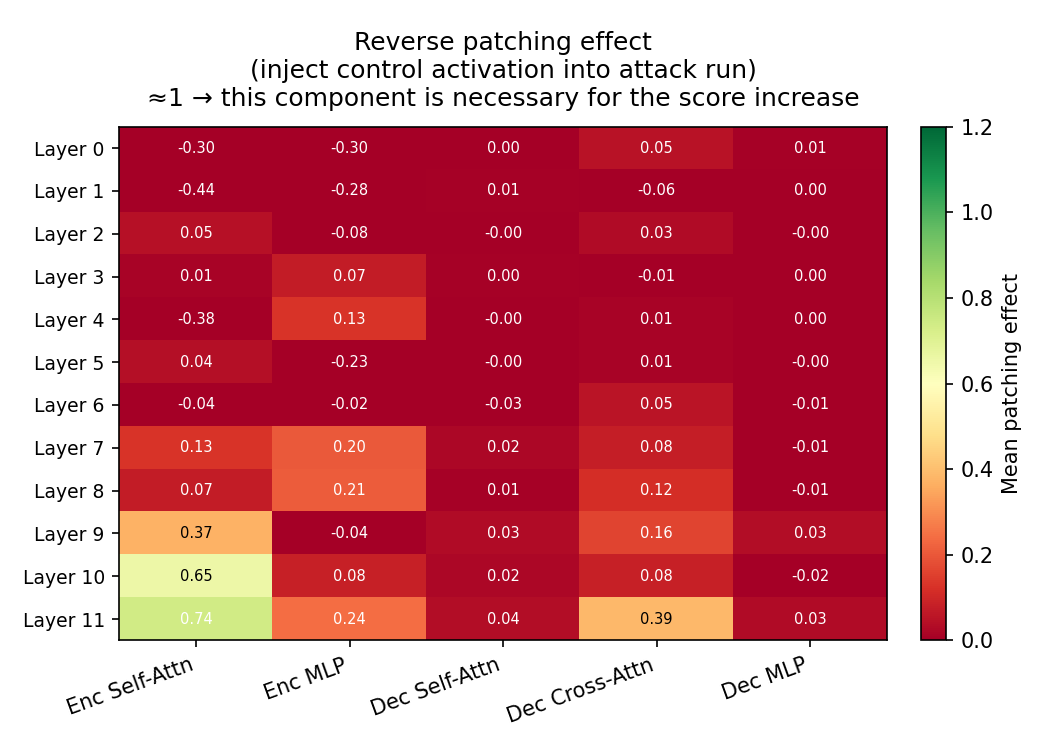
\includegraphics[width=0.17\textwidth]{outputs/attacks/important_end_5/plots/reverse_layer_component_heatmap.png} \\[4pt]
\rotatebox{90}{\textbf{combined}} & 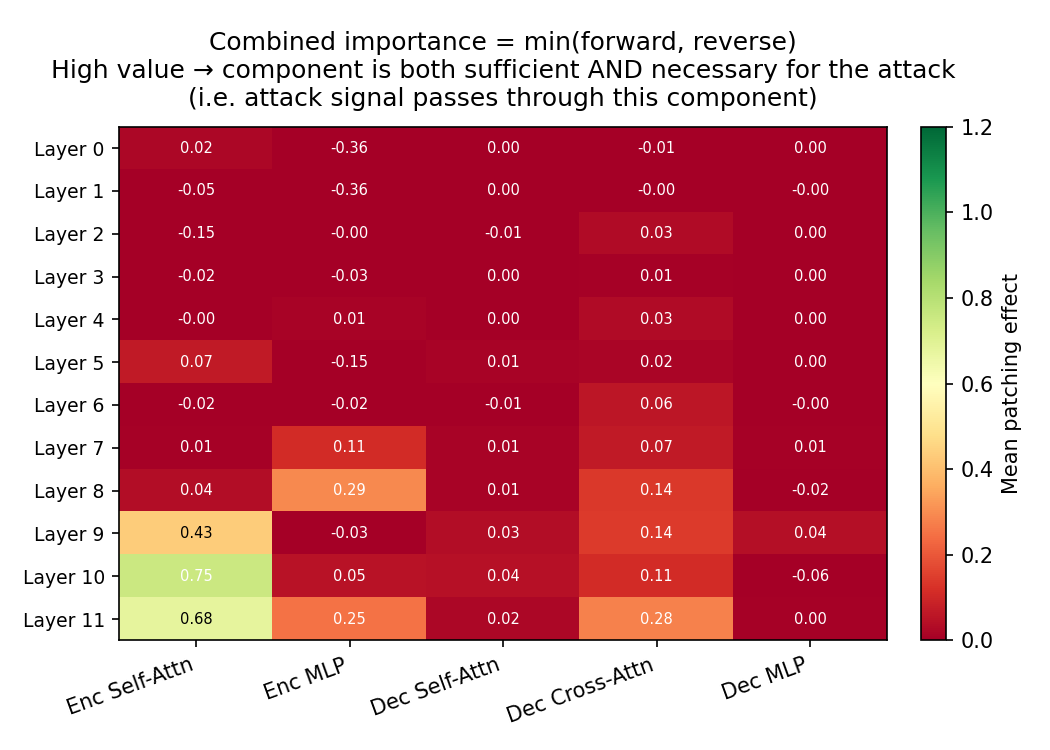
\includegraphics[width=0.17\textwidth]{outputs/attacks/important_end_1/plots/combined_layer_component_heatmap.png} & 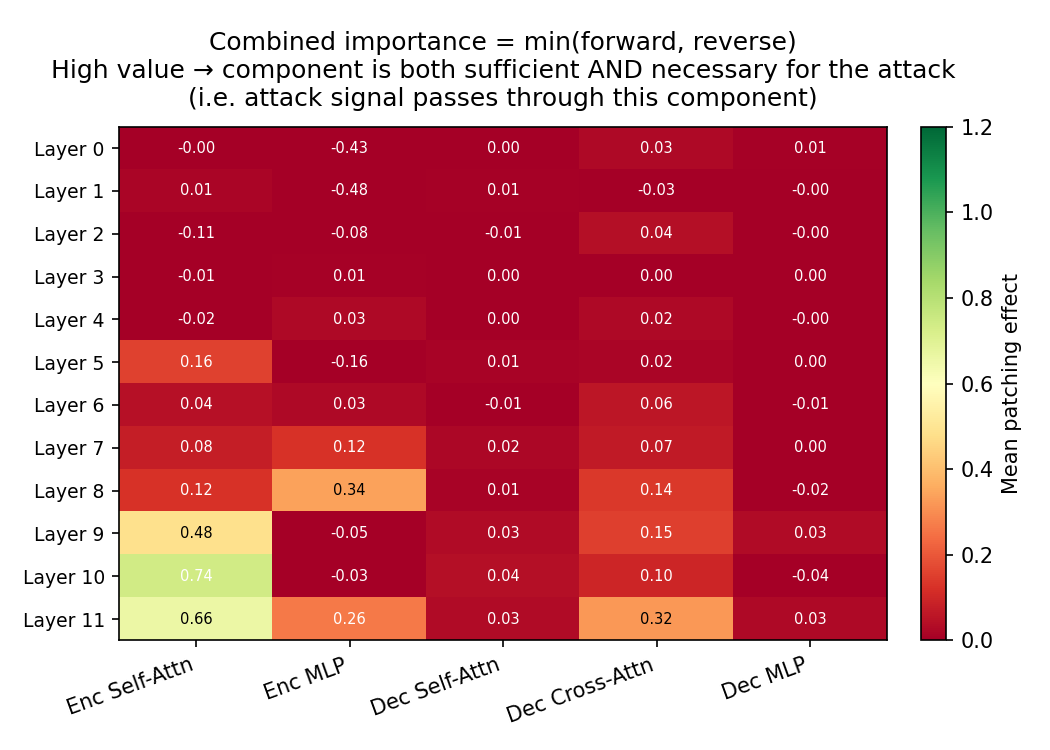
\includegraphics[width=0.17\textwidth]{outputs/attacks/important_end_2/plots/combined_layer_component_heatmap.png} & 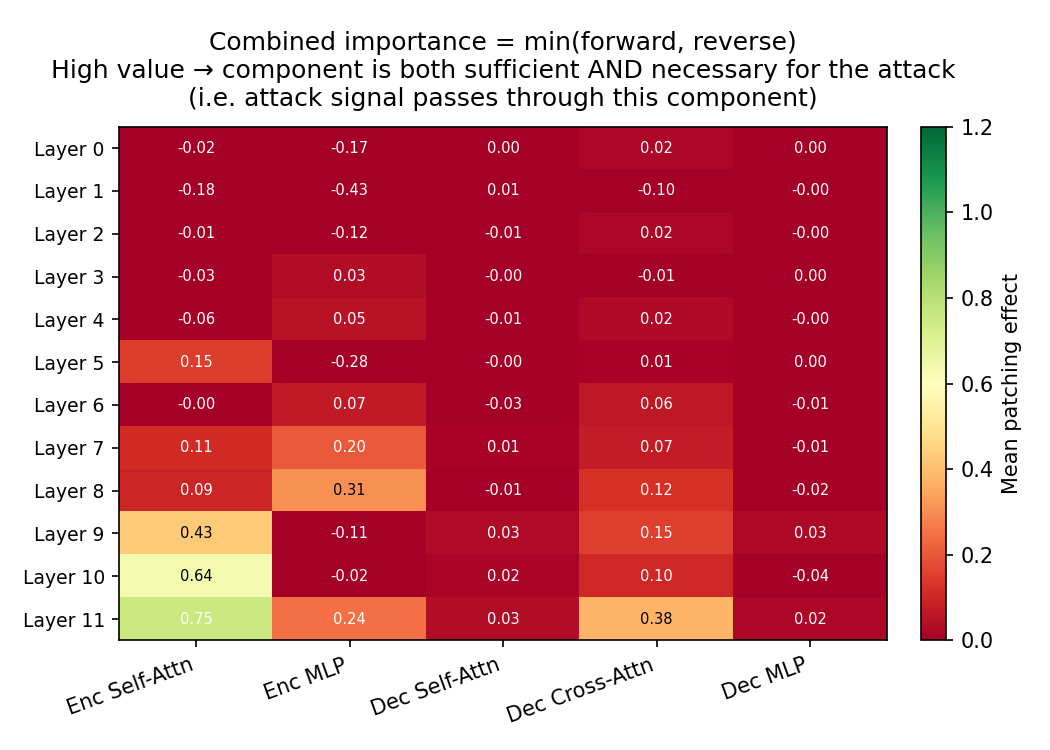
\includegraphics[width=0.17\textwidth]{outputs/attacks/important_end_3/plots/combined_layer_component_heatmap.png} & 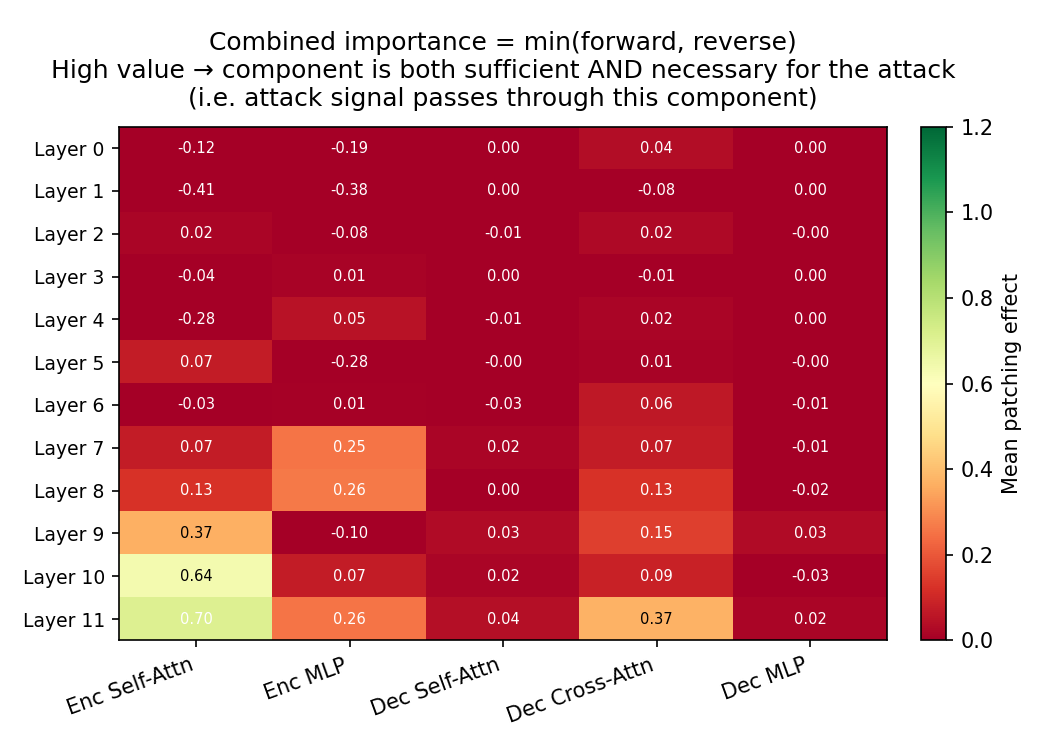
\includegraphics[width=0.17\textwidth]{outputs/attacks/important_end_4/plots/combined_layer_component_heatmap.png} & 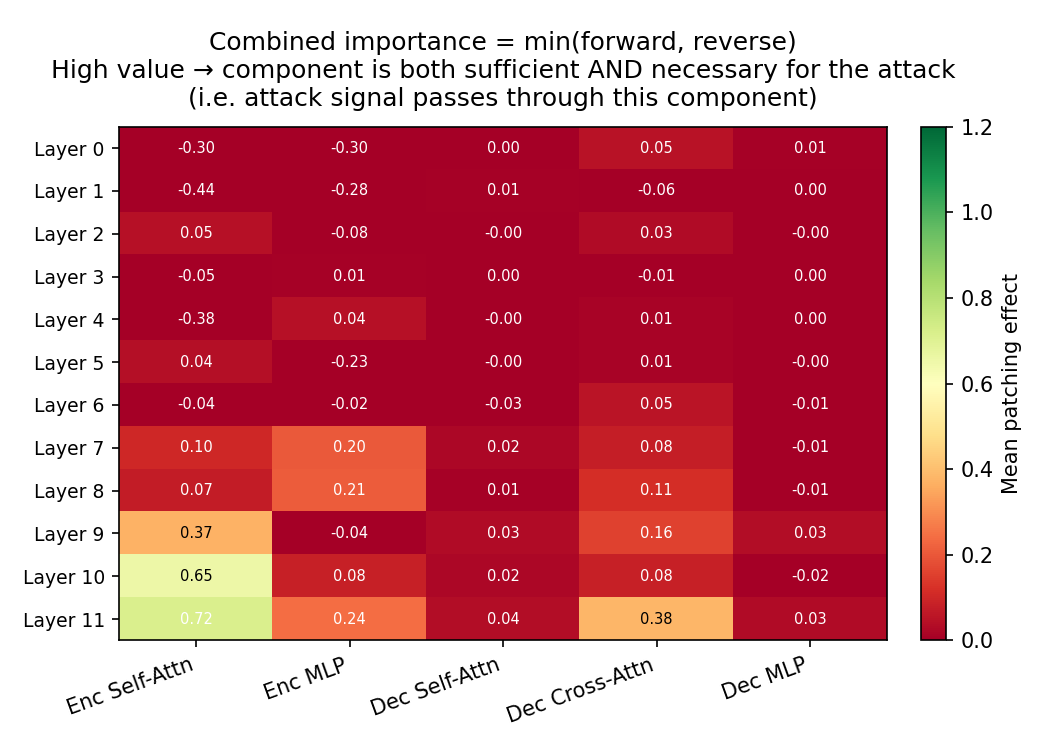
\includegraphics[width=0.17\textwidth]{outputs/attacks/important_end_5/plots/combined_layer_component_heatmap.png} \\[4pt]
\end{tabular}
\caption{Patching heatmaps for \texttt{important_end}: forward (top), reverse (middle), combined (bottom) across repetitions 1--5.}
\label{fig:hm:important_end}
\end{figure}

\begin{figure}[H]
\centering
\setlength{\tabcolsep}{2pt}
\renewcommand{\arraystretch}{0.5}
\begin{tabular}{r ccccc}
& \textbf{rep=1} & \textbf{rep=2} & \textbf{rep=3} & \textbf{rep=4} & \textbf{rep=5} \\[2pt]
\rotatebox{90}{\textbf{forward}} & 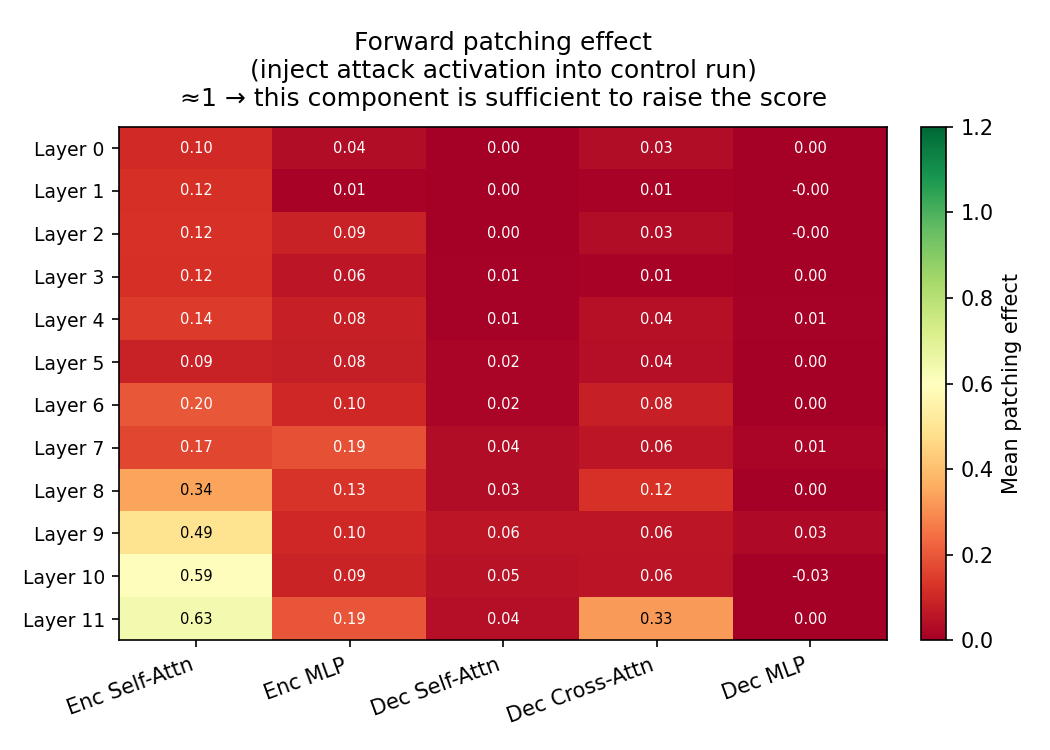
\includegraphics[width=0.17\textwidth]{outputs/attacks/important_random_1/plots/forward_layer_component_heatmap.png} & 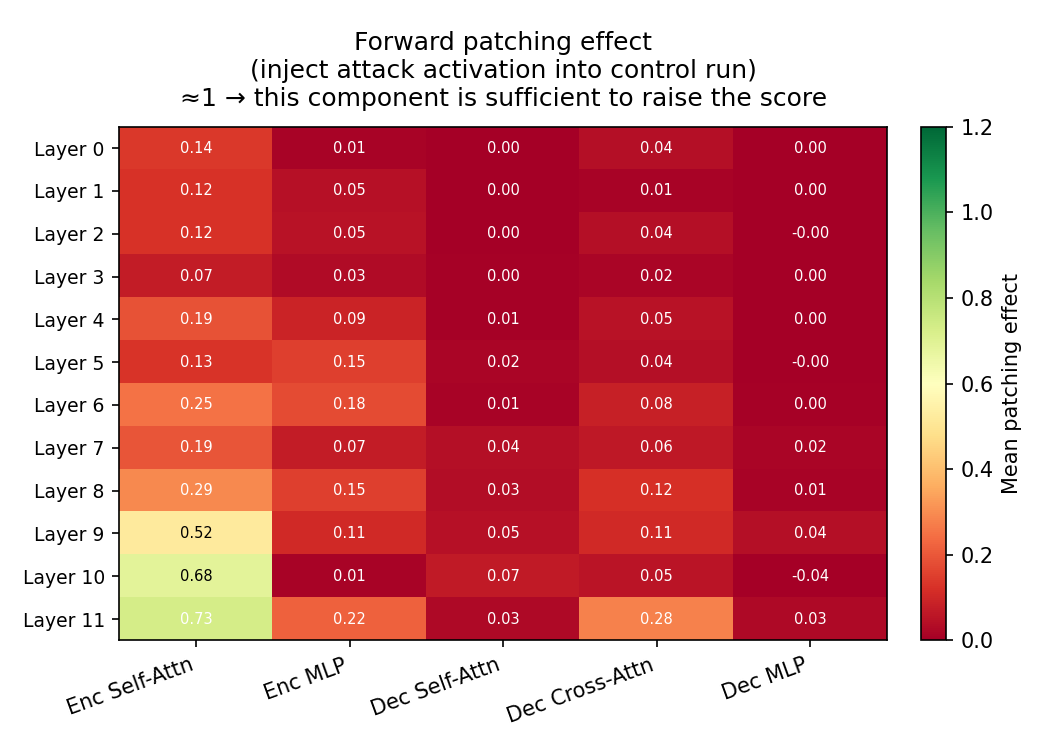
\includegraphics[width=0.17\textwidth]{outputs/attacks/important_random_2/plots/forward_layer_component_heatmap.png} & 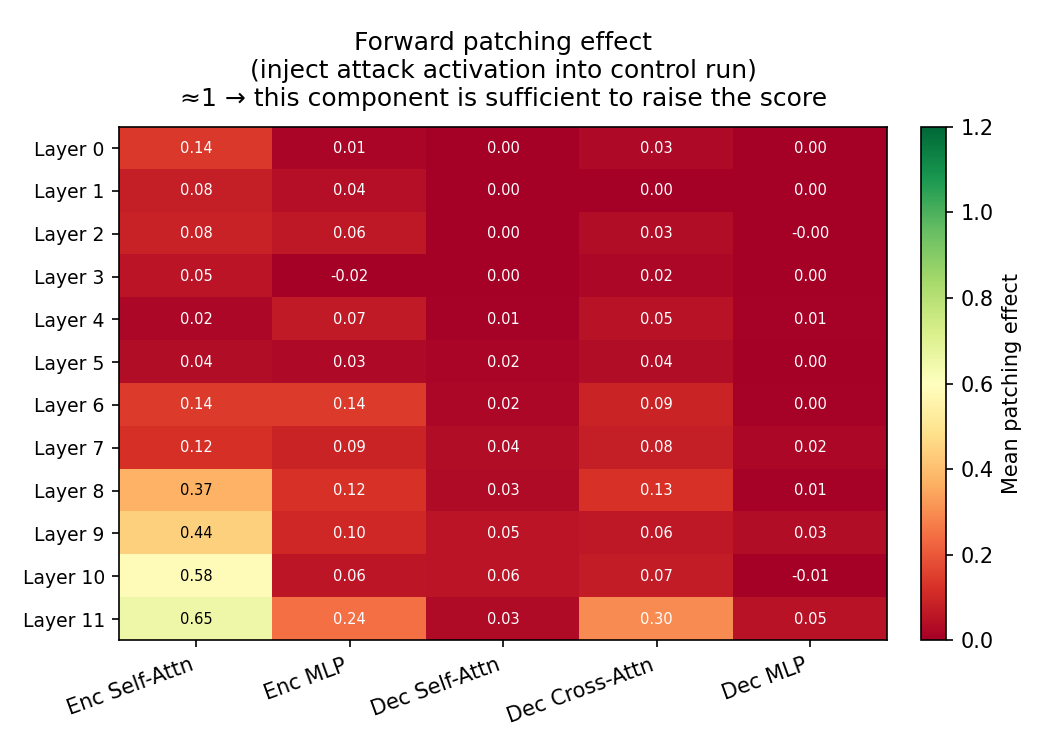
\includegraphics[width=0.17\textwidth]{outputs/attacks/important_random_3/plots/forward_layer_component_heatmap.png} & 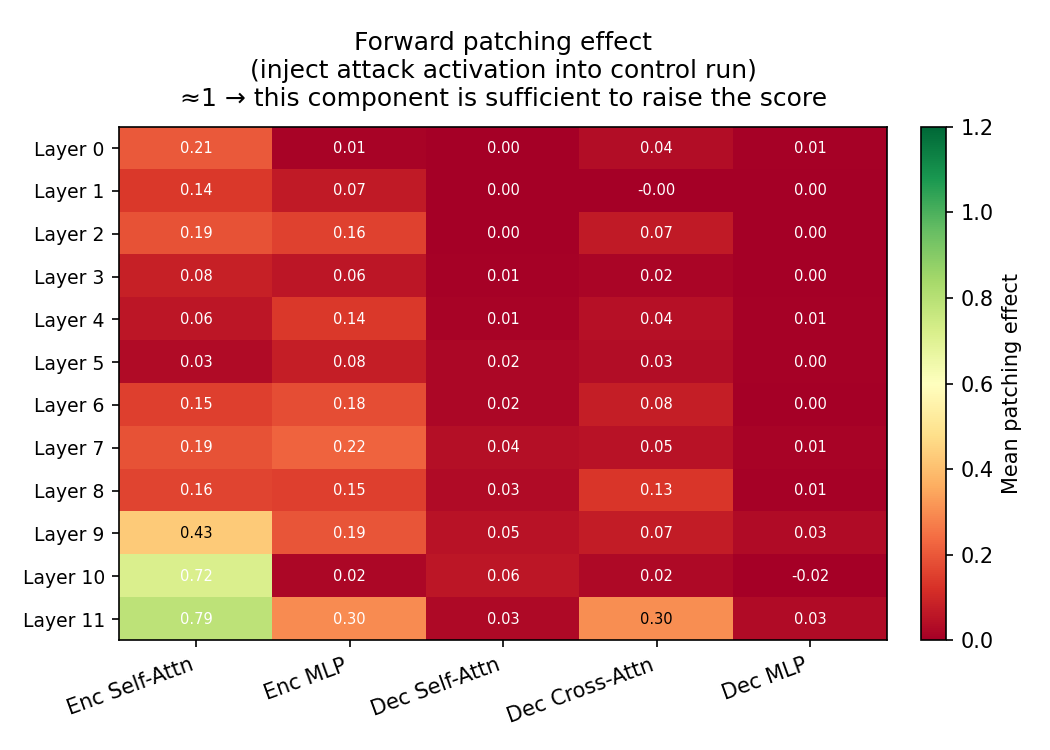
\includegraphics[width=0.17\textwidth]{outputs/attacks/important_random_4/plots/forward_layer_component_heatmap.png} & 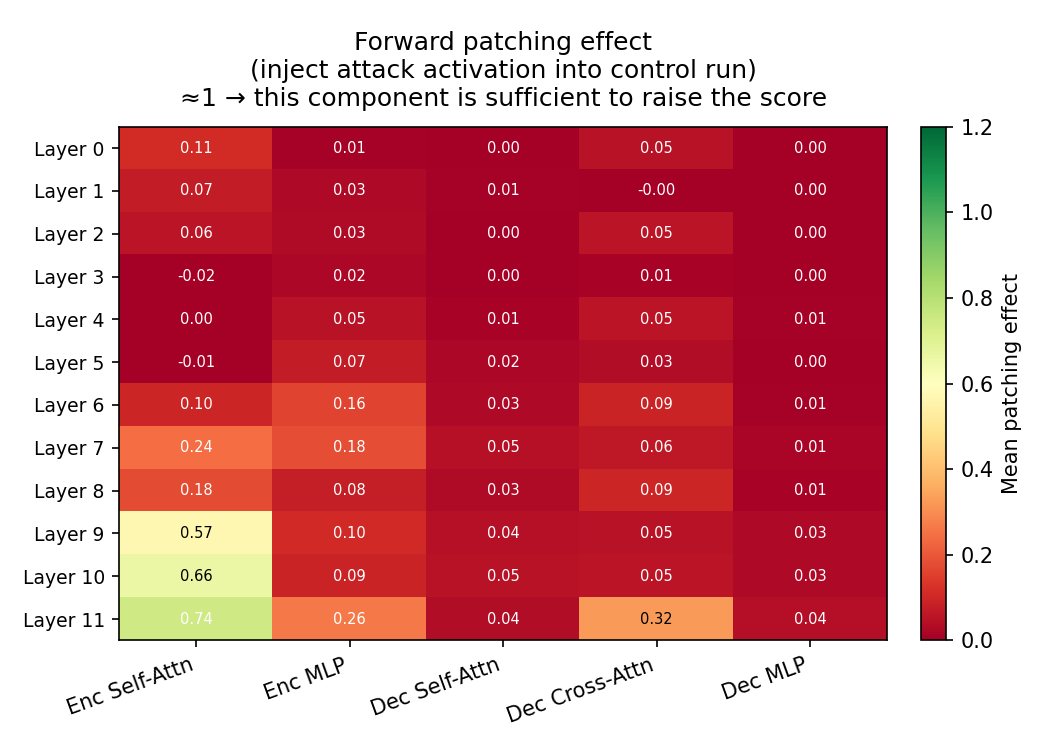
\includegraphics[width=0.17\textwidth]{outputs/attacks/important_random_5/plots/forward_layer_component_heatmap.png} \\[4pt]
\rotatebox{90}{\textbf{reverse}} & 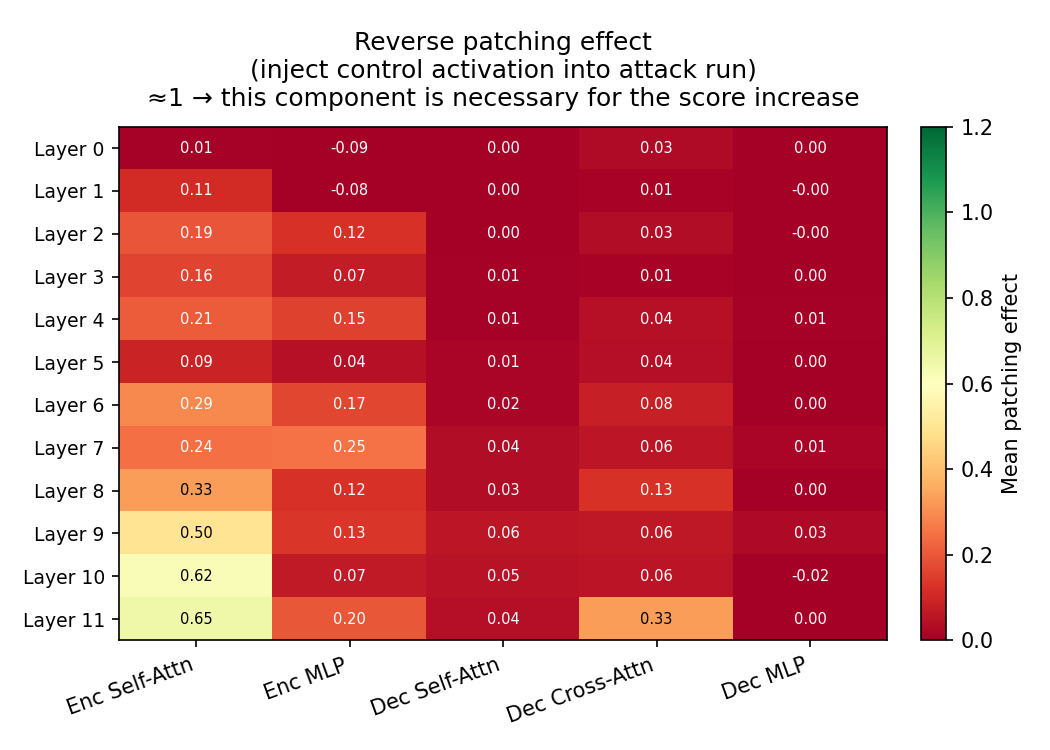
\includegraphics[width=0.17\textwidth]{outputs/attacks/important_random_1/plots/reverse_layer_component_heatmap.png} & 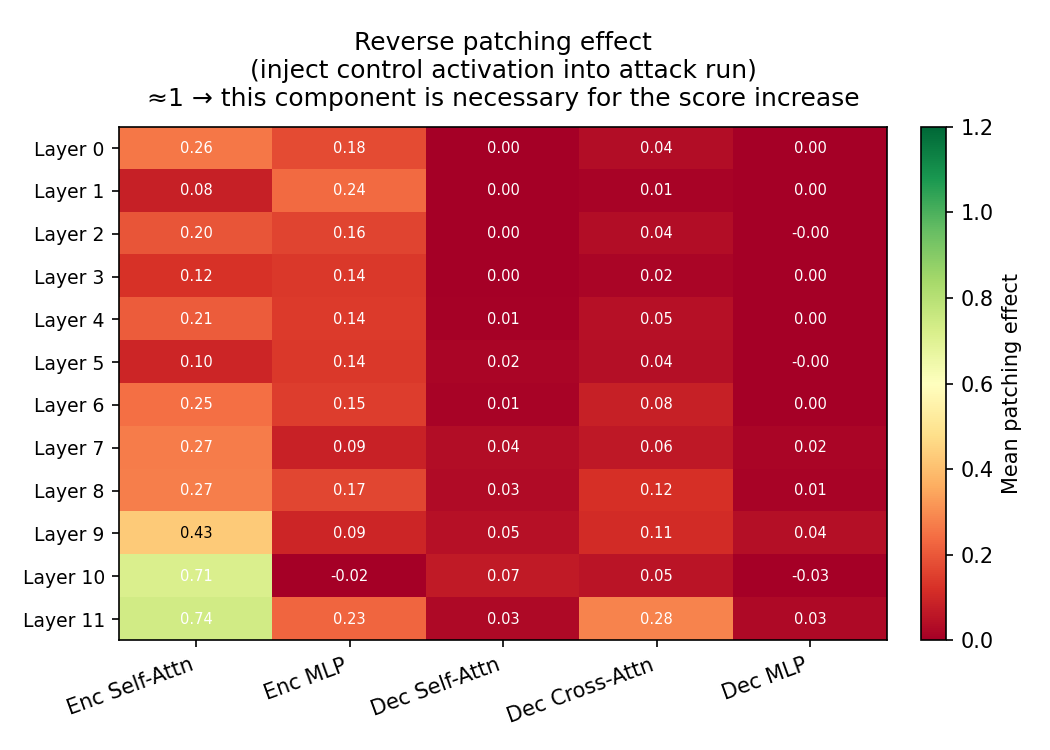
\includegraphics[width=0.17\textwidth]{outputs/attacks/important_random_2/plots/reverse_layer_component_heatmap.png} & 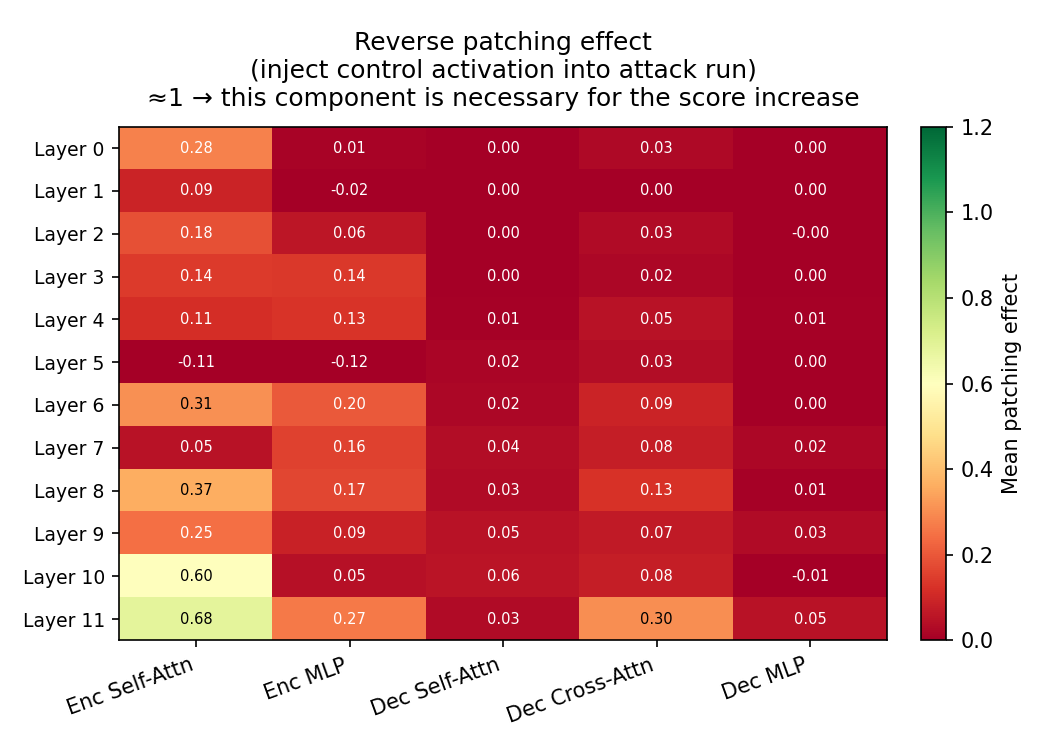
\includegraphics[width=0.17\textwidth]{outputs/attacks/important_random_3/plots/reverse_layer_component_heatmap.png} & 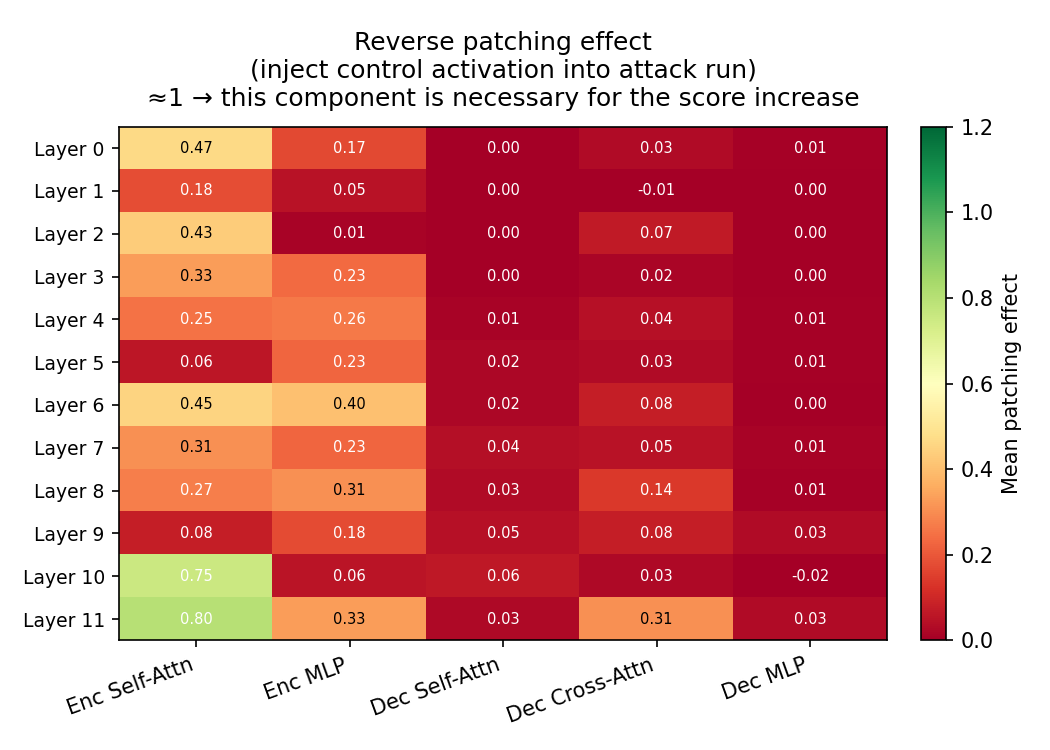
\includegraphics[width=0.17\textwidth]{outputs/attacks/important_random_4/plots/reverse_layer_component_heatmap.png} & 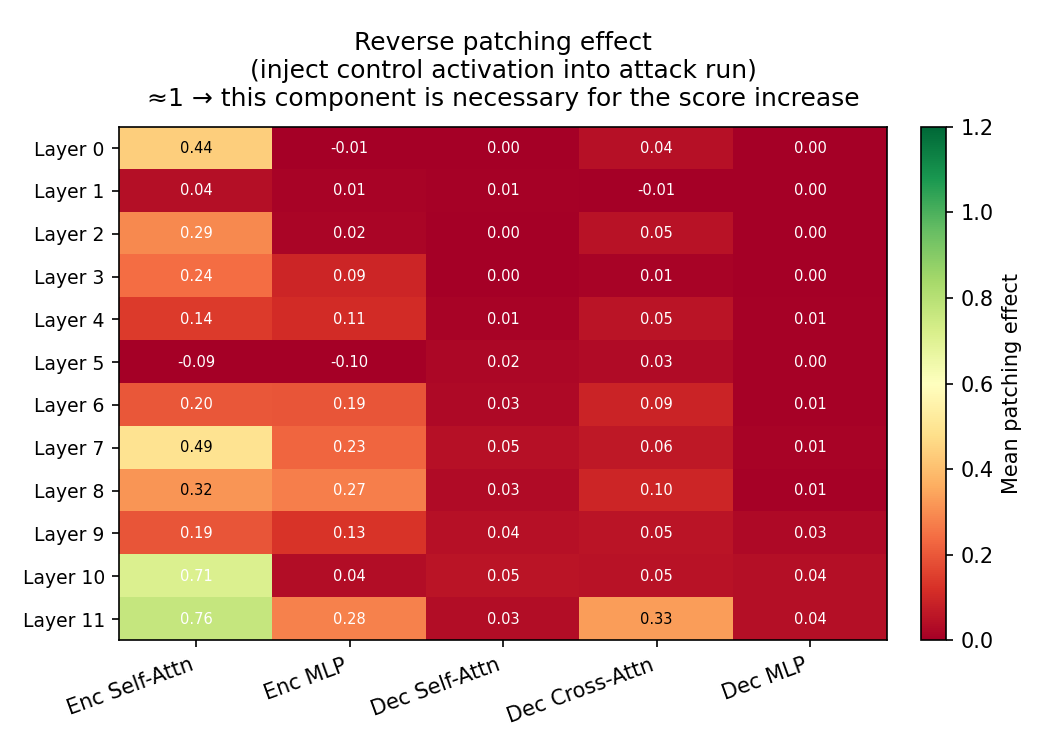
\includegraphics[width=0.17\textwidth]{outputs/attacks/important_random_5/plots/reverse_layer_component_heatmap.png} \\[4pt]
\rotatebox{90}{\textbf{combined}} & 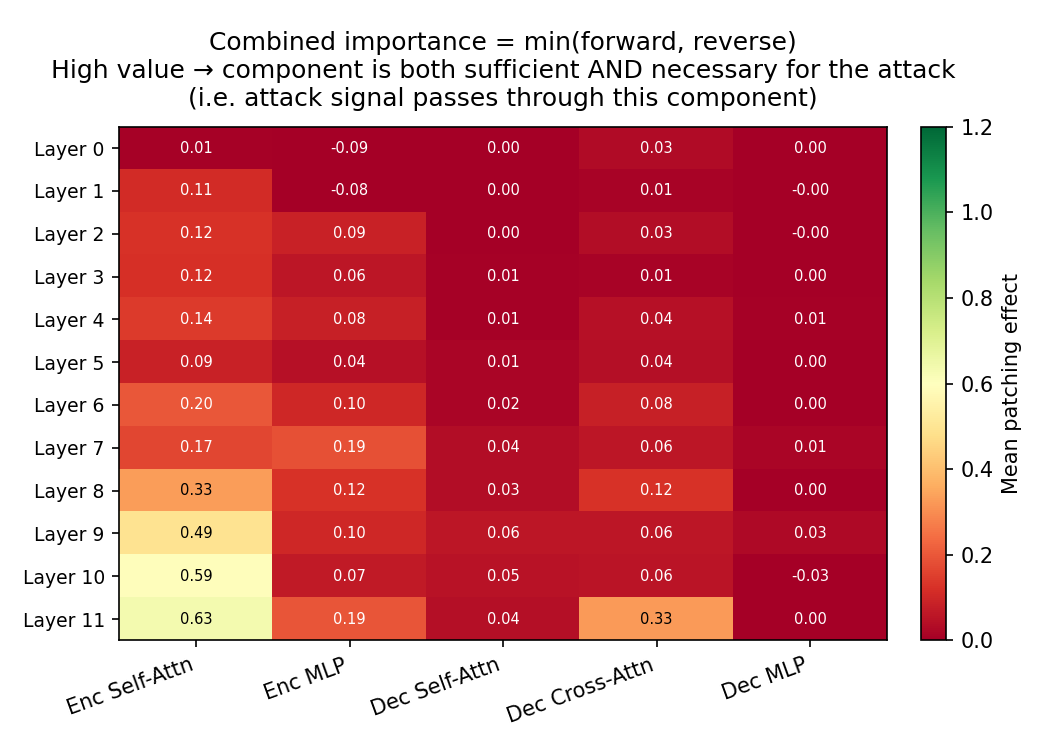
\includegraphics[width=0.17\textwidth]{outputs/attacks/important_random_1/plots/combined_layer_component_heatmap.png} & 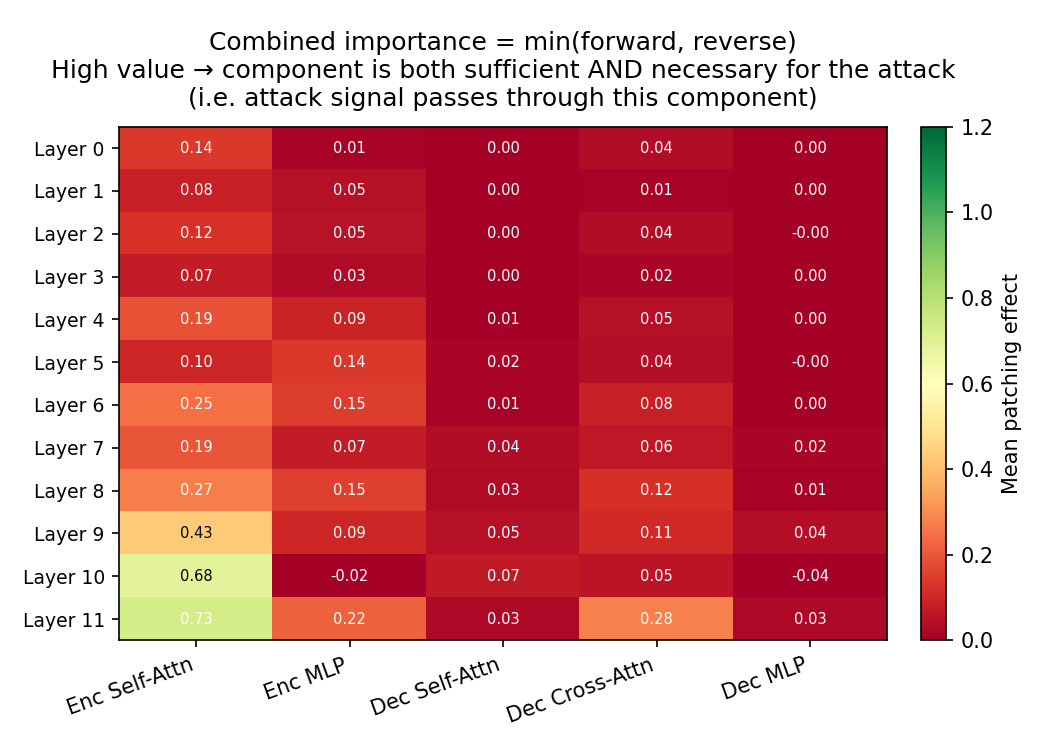
\includegraphics[width=0.17\textwidth]{outputs/attacks/important_random_2/plots/combined_layer_component_heatmap.png} & 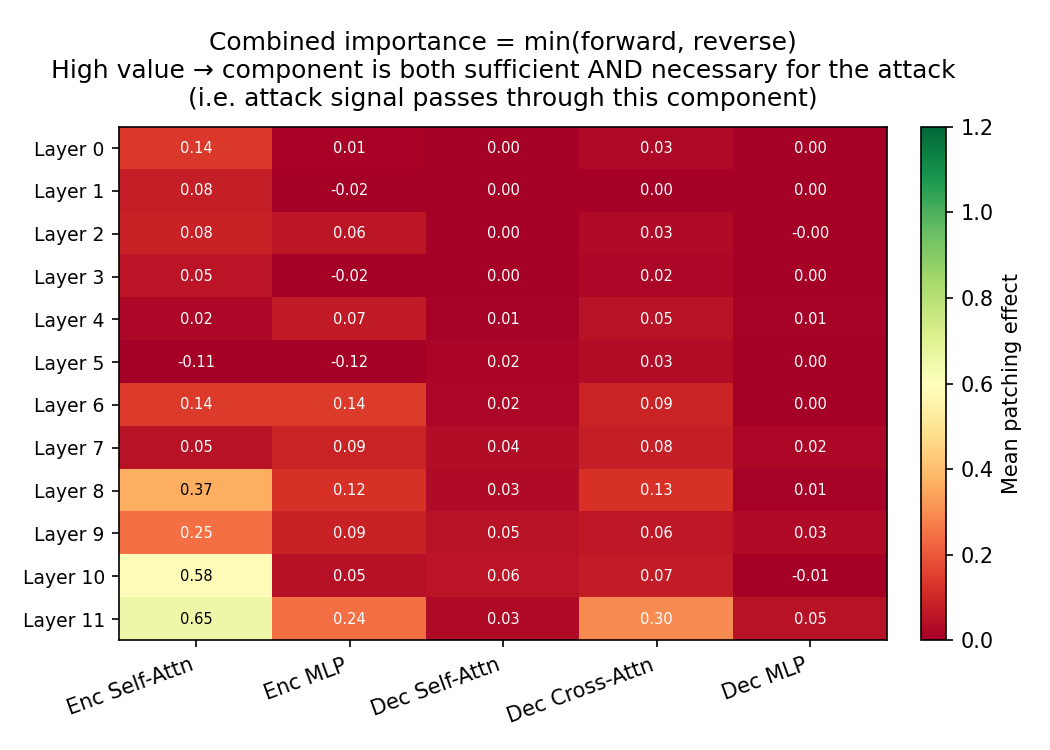
\includegraphics[width=0.17\textwidth]{outputs/attacks/important_random_3/plots/combined_layer_component_heatmap.png} & 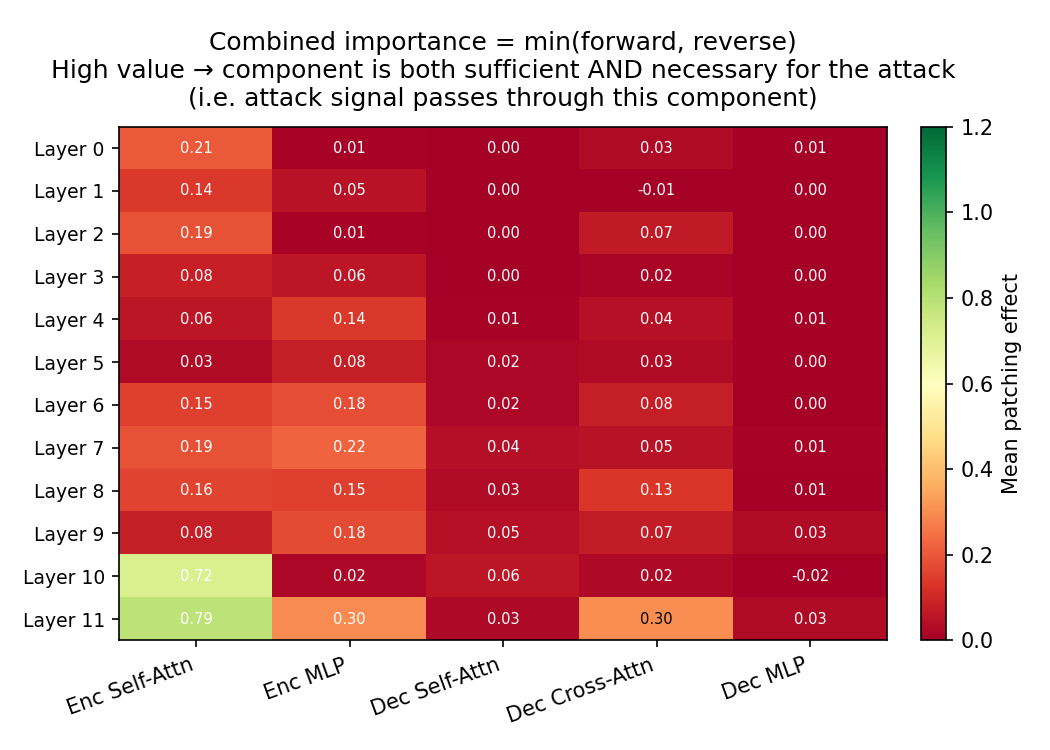
\includegraphics[width=0.17\textwidth]{outputs/attacks/important_random_4/plots/combined_layer_component_heatmap.png} & 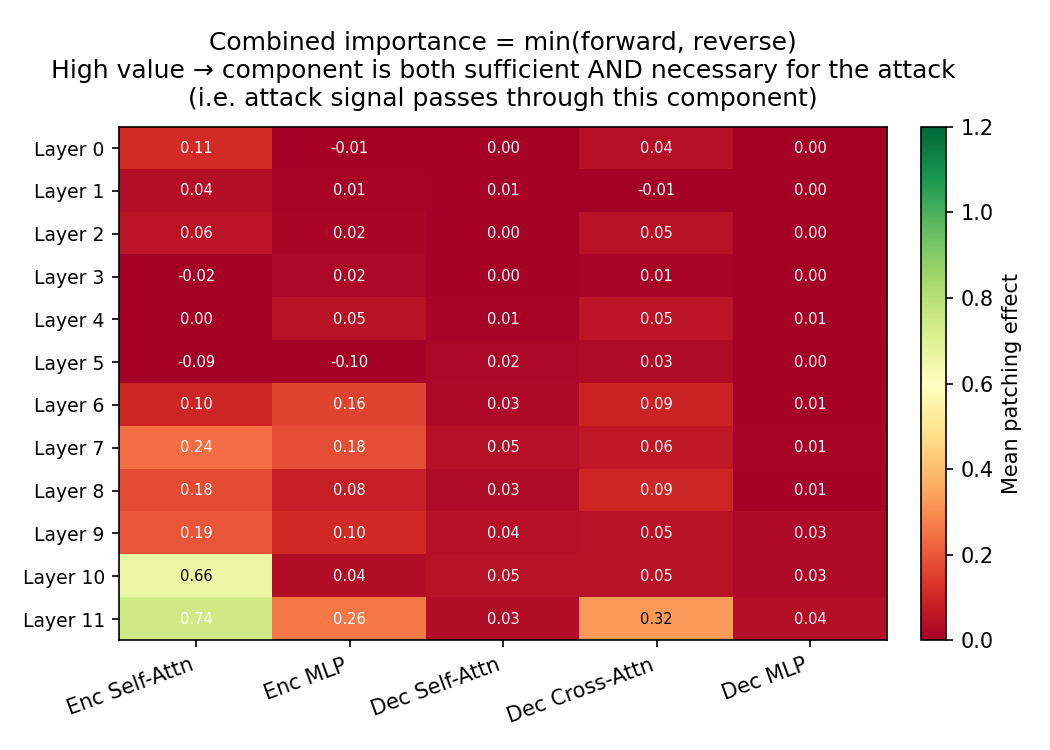
\includegraphics[width=0.17\textwidth]{outputs/attacks/important_random_5/plots/combined_layer_component_heatmap.png} \\[4pt]
\end{tabular}
\caption{Patching heatmaps for \texttt{important_random}: forward (top), reverse (middle), combined (bottom) across repetitions 1--5.}
\label{fig:hm:important_random}
\end{figure}

\begin{figure}[H]
\centering
\setlength{\tabcolsep}{2pt}
\renewcommand{\arraystretch}{0.5}
\begin{tabular}{r ccccc}
& \textbf{rep=1} & \textbf{rep=2} & \textbf{rep=3} & \textbf{rep=4} & \textbf{rep=5} \\[2pt]
\rotatebox{90}{\textbf{forward}} & 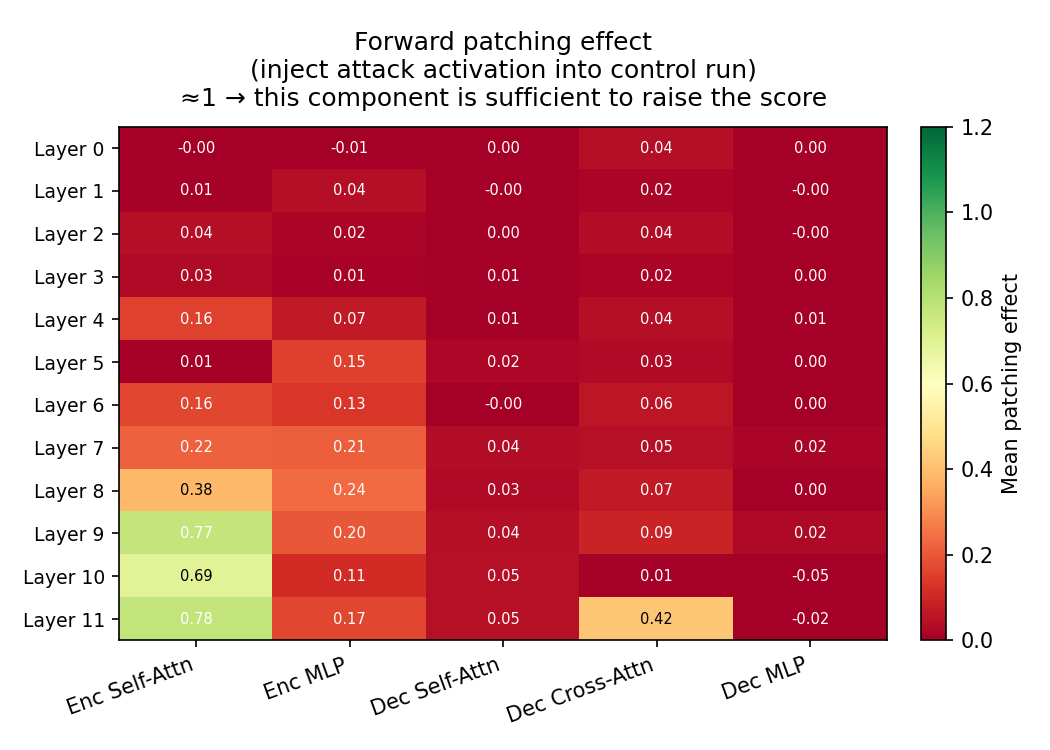
\includegraphics[width=0.17\textwidth]{outputs/attacks/important_start_1/plots/forward_layer_component_heatmap.png} & 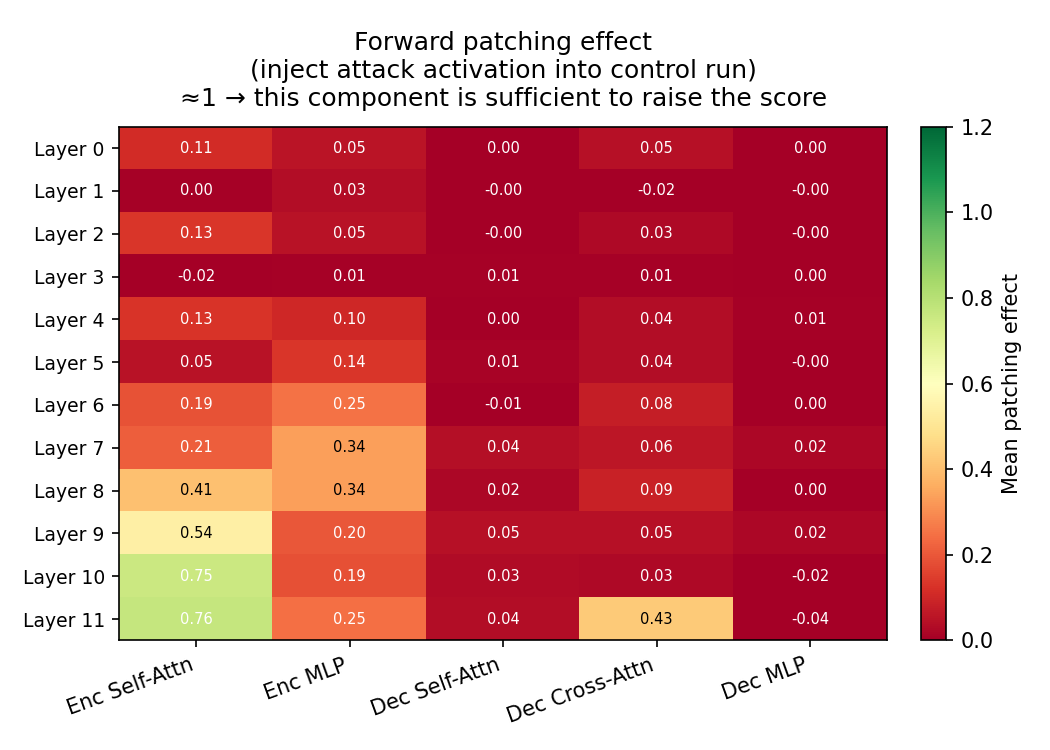
\includegraphics[width=0.17\textwidth]{outputs/attacks/important_start_2/plots/forward_layer_component_heatmap.png} & 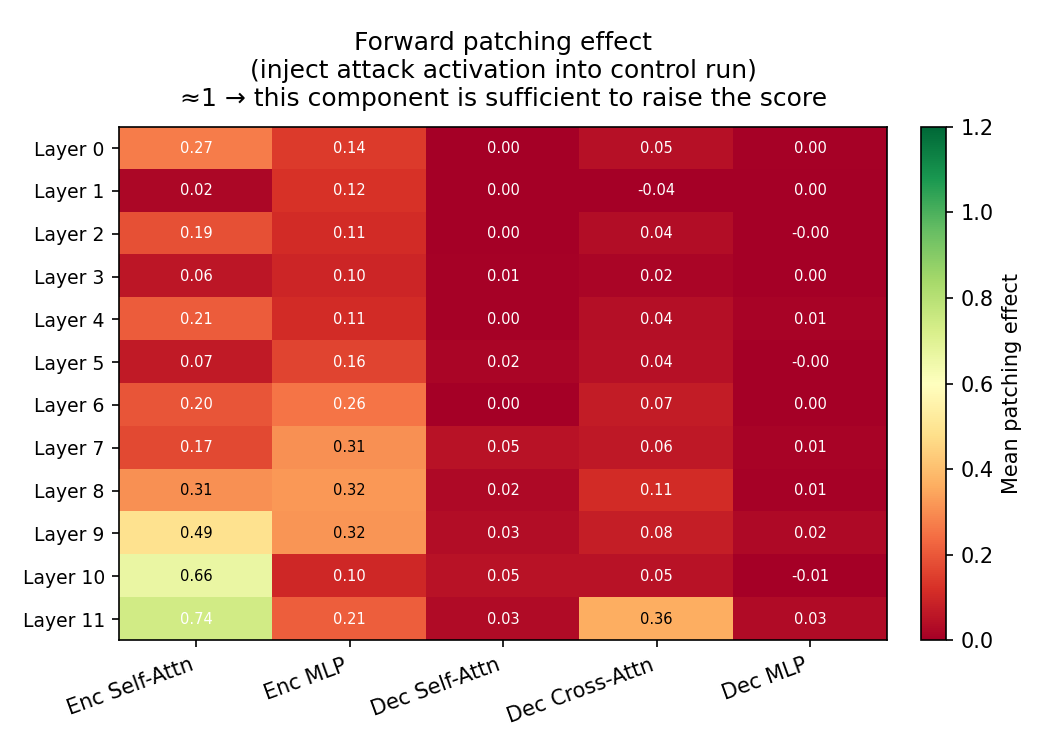
\includegraphics[width=0.17\textwidth]{outputs/attacks/important_start_3/plots/forward_layer_component_heatmap.png} & 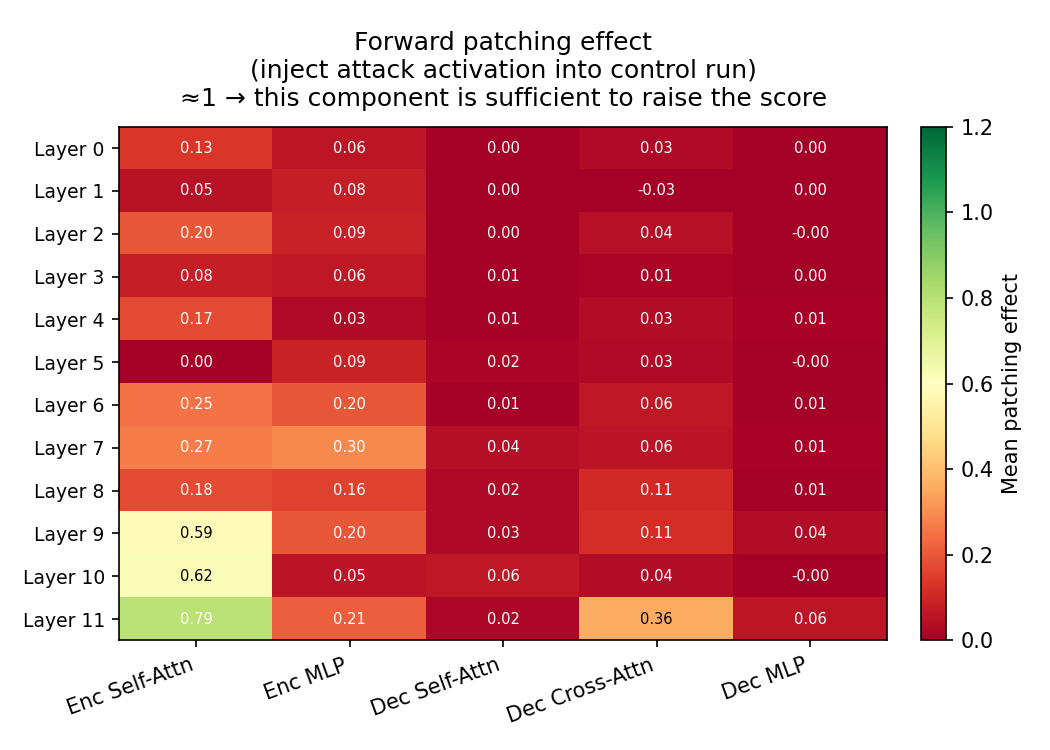
\includegraphics[width=0.17\textwidth]{outputs/attacks/important_start_4/plots/forward_layer_component_heatmap.png} & 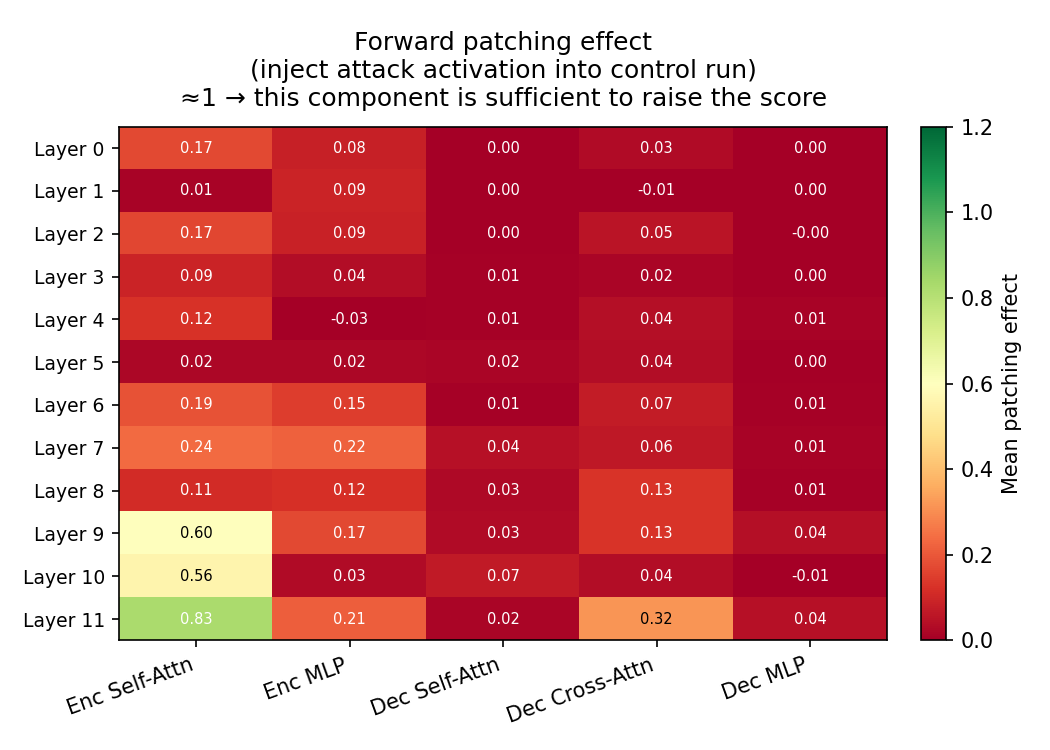
\includegraphics[width=0.17\textwidth]{outputs/attacks/important_start_5/plots/forward_layer_component_heatmap.png} \\[4pt]
\rotatebox{90}{\textbf{reverse}} & 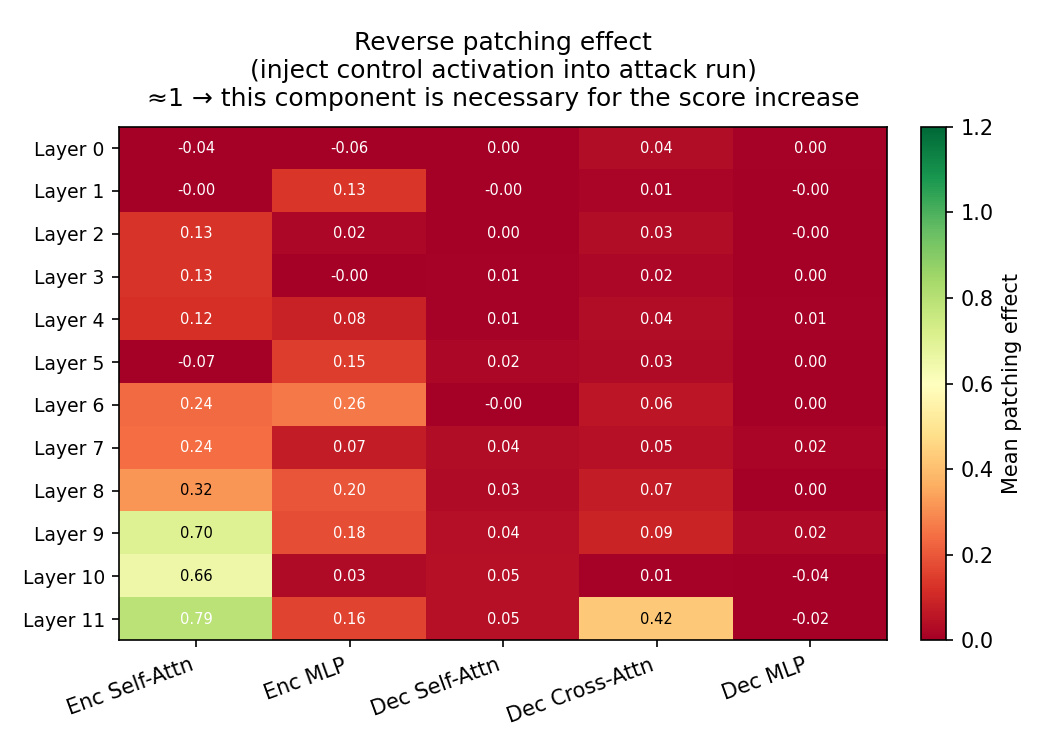
\includegraphics[width=0.17\textwidth]{outputs/attacks/important_start_1/plots/reverse_layer_component_heatmap.png} & 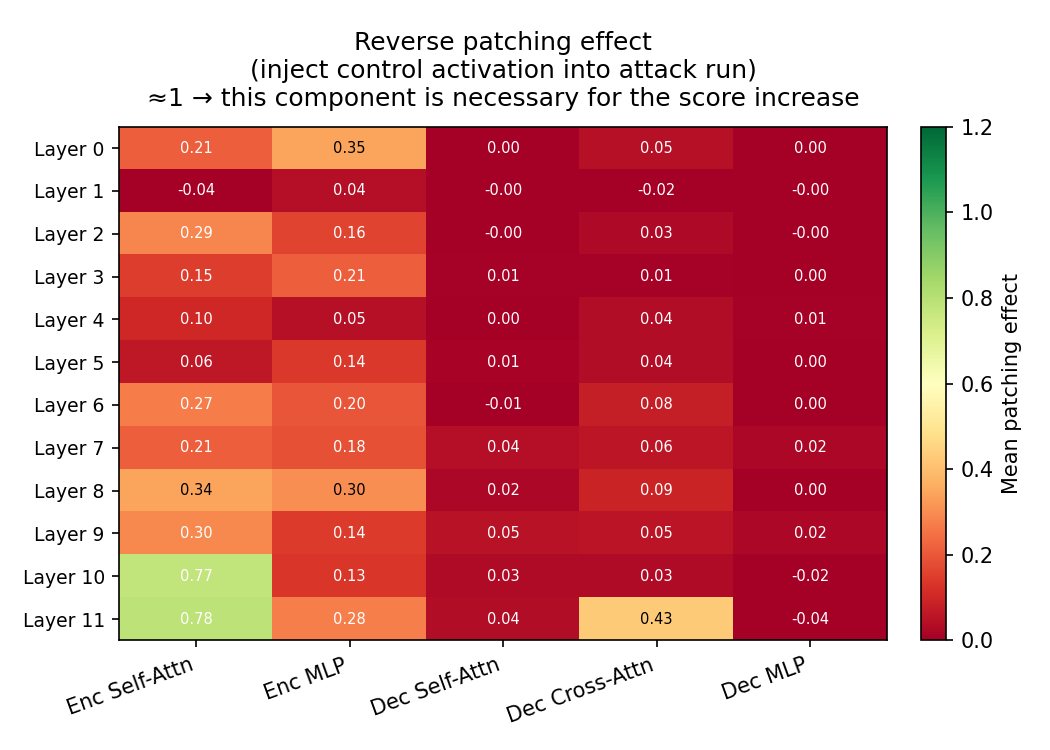
\includegraphics[width=0.17\textwidth]{outputs/attacks/important_start_2/plots/reverse_layer_component_heatmap.png} & 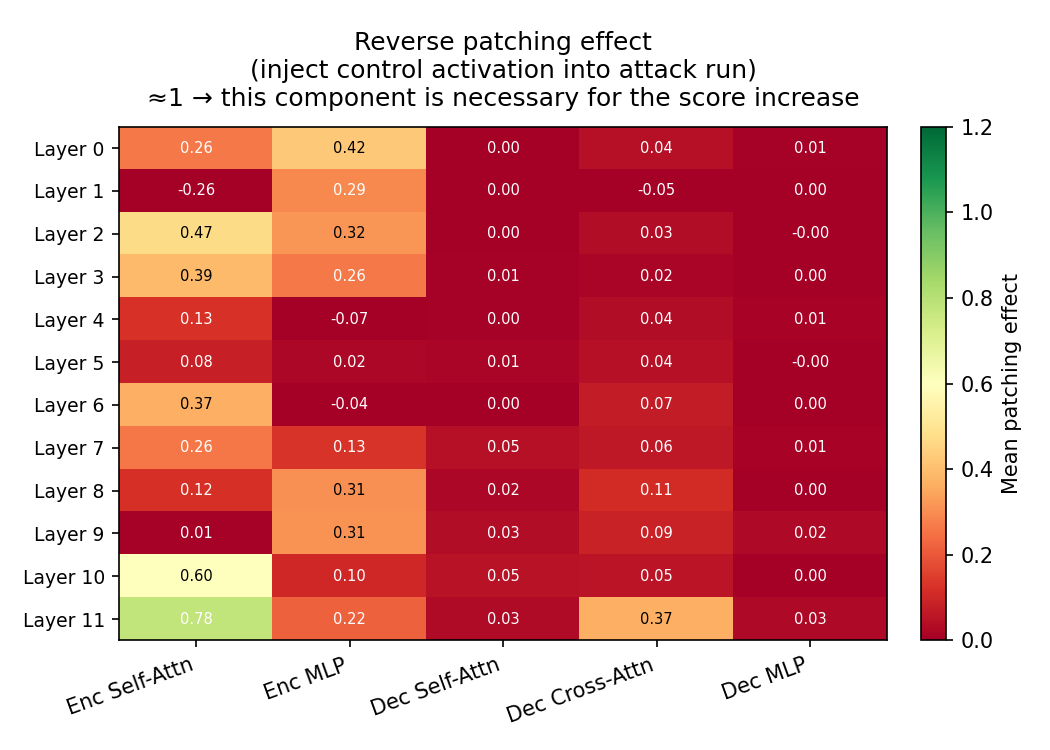
\includegraphics[width=0.17\textwidth]{outputs/attacks/important_start_3/plots/reverse_layer_component_heatmap.png} & 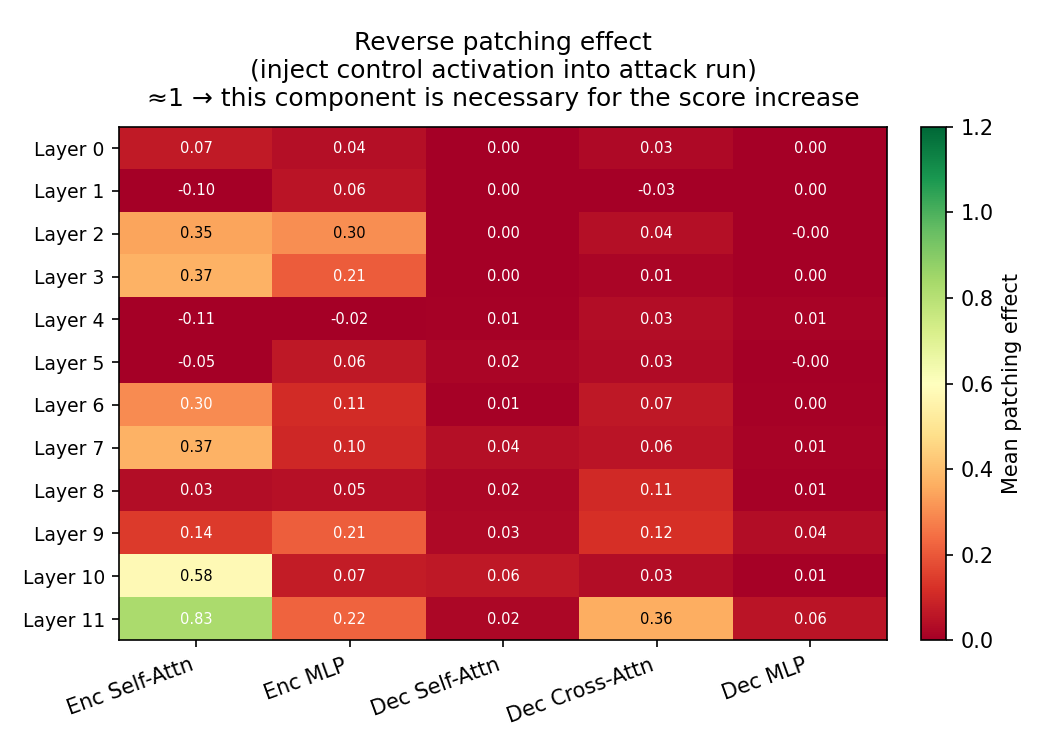
\includegraphics[width=0.17\textwidth]{outputs/attacks/important_start_4/plots/reverse_layer_component_heatmap.png} & 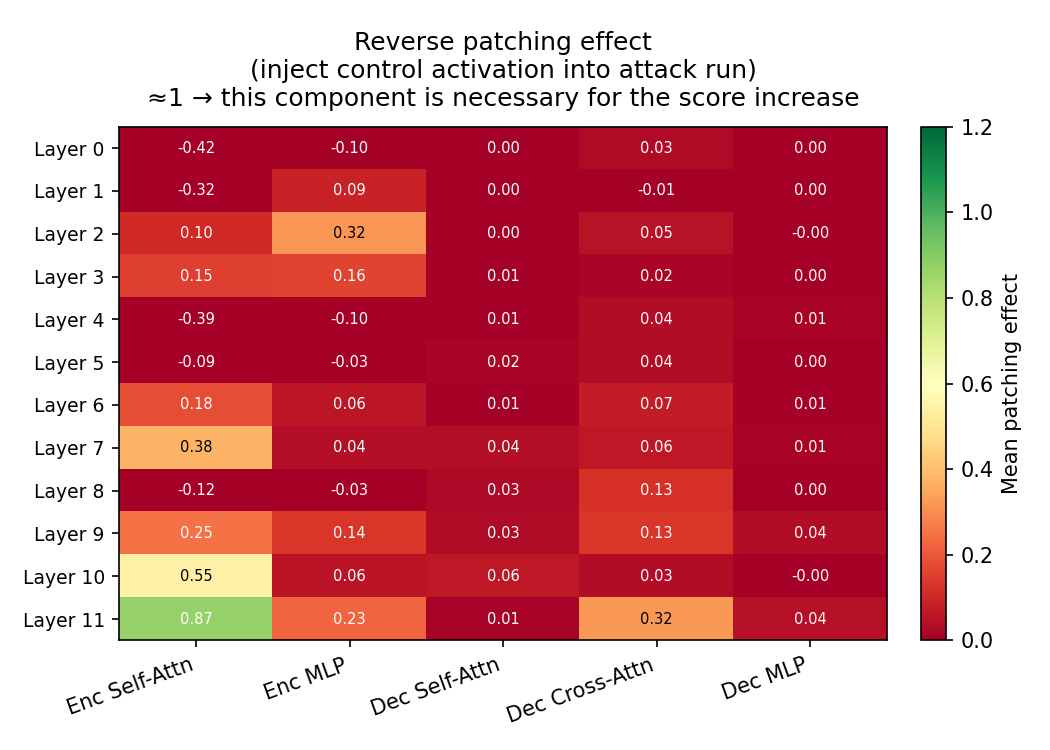
\includegraphics[width=0.17\textwidth]{outputs/attacks/important_start_5/plots/reverse_layer_component_heatmap.png} \\[4pt]
\rotatebox{90}{\textbf{combined}} & 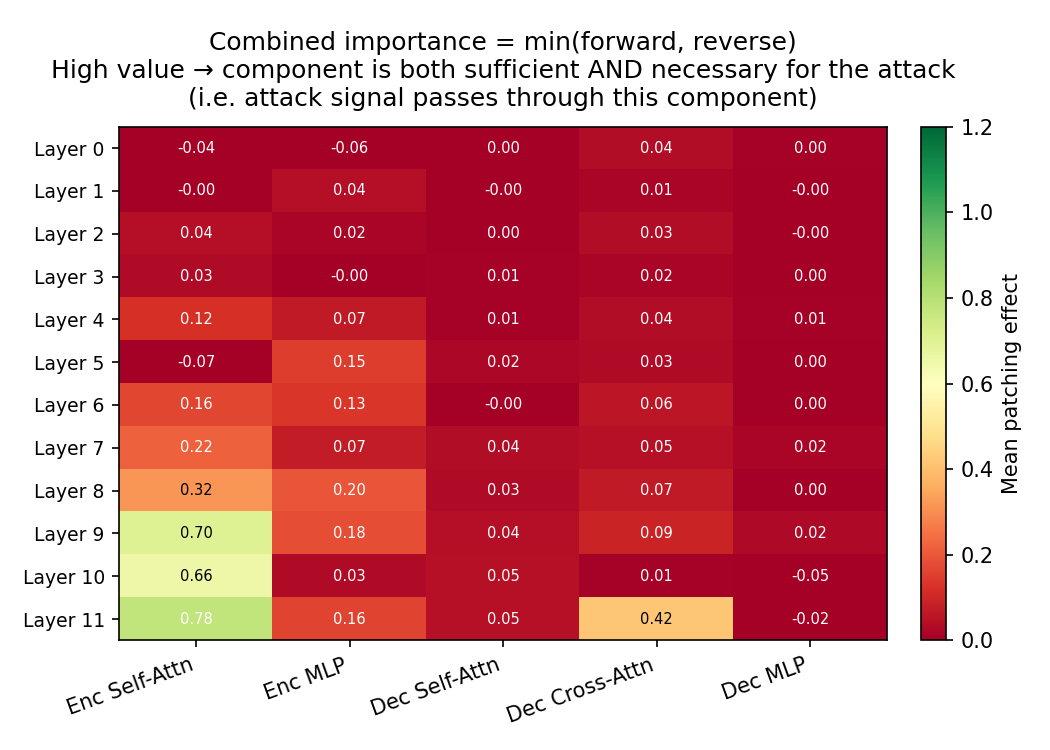
\includegraphics[width=0.17\textwidth]{outputs/attacks/important_start_1/plots/combined_layer_component_heatmap.png} & 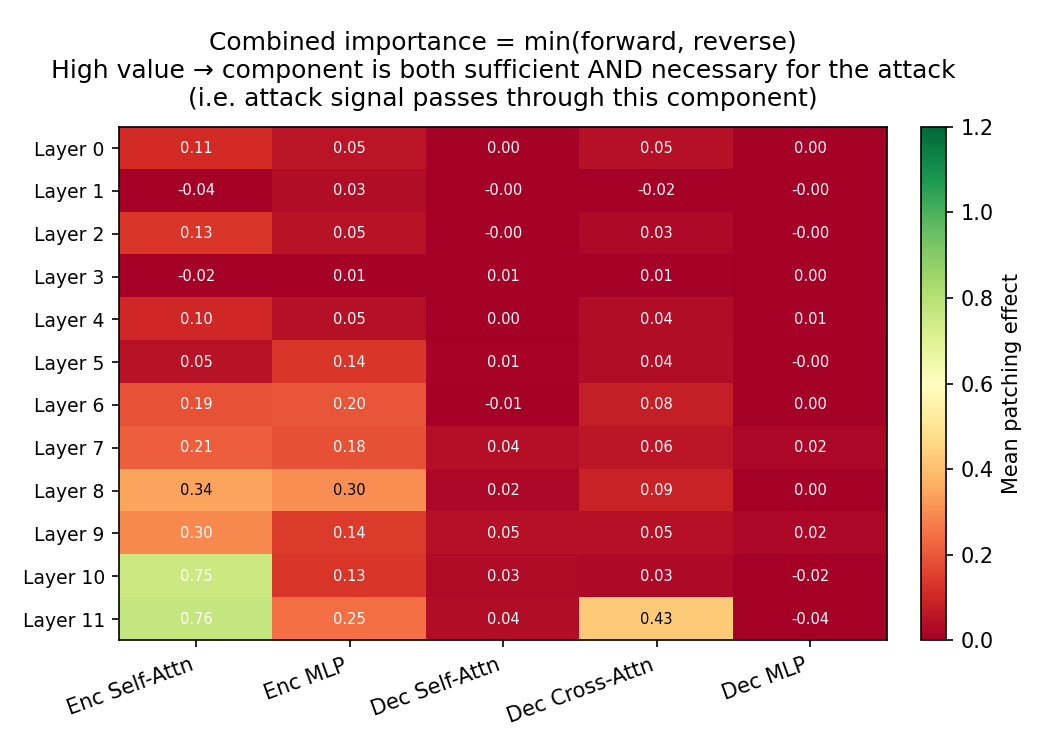
\includegraphics[width=0.17\textwidth]{outputs/attacks/important_start_2/plots/combined_layer_component_heatmap.png} & 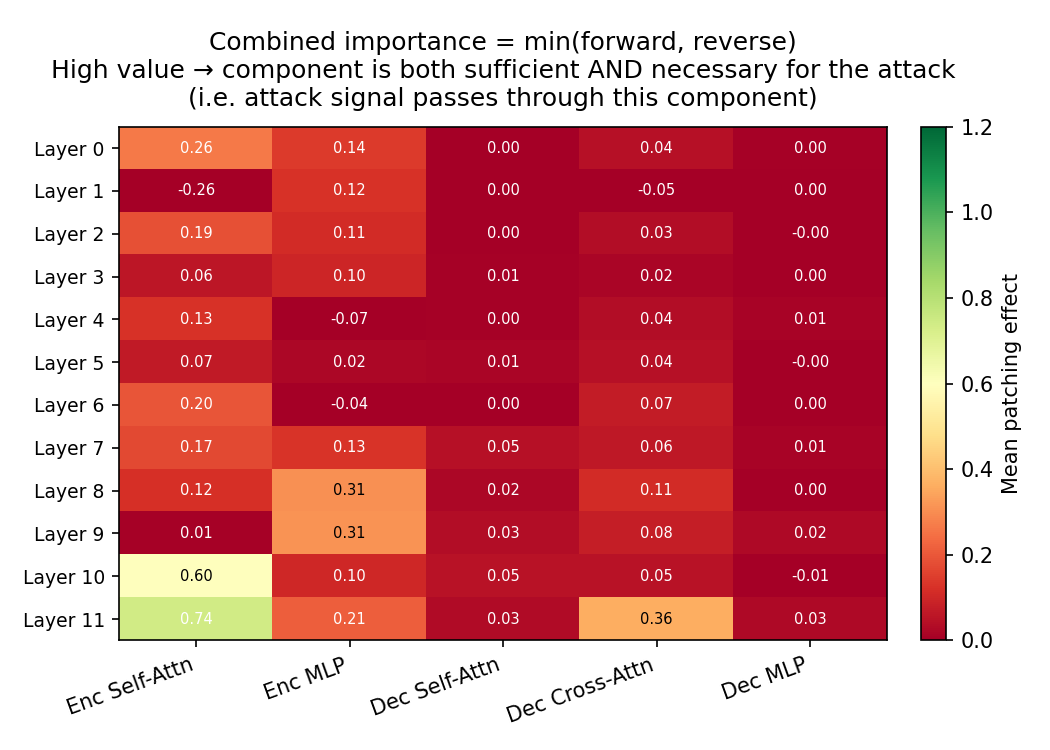
\includegraphics[width=0.17\textwidth]{outputs/attacks/important_start_3/plots/combined_layer_component_heatmap.png} & 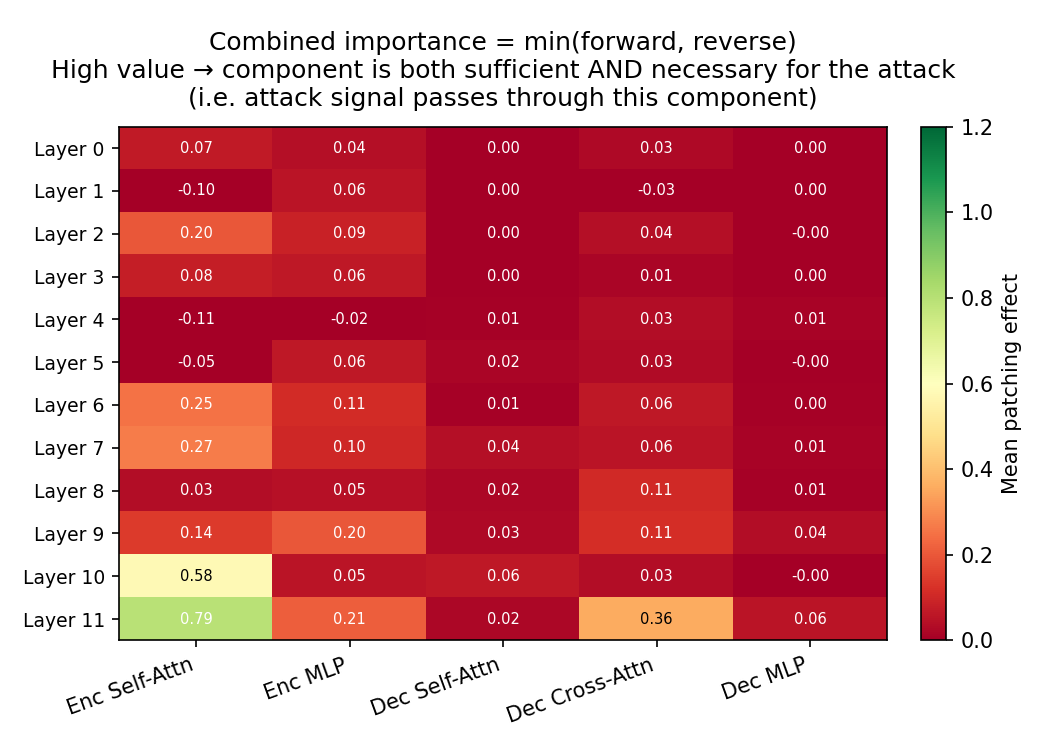
\includegraphics[width=0.17\textwidth]{outputs/attacks/important_start_4/plots/combined_layer_component_heatmap.png} & 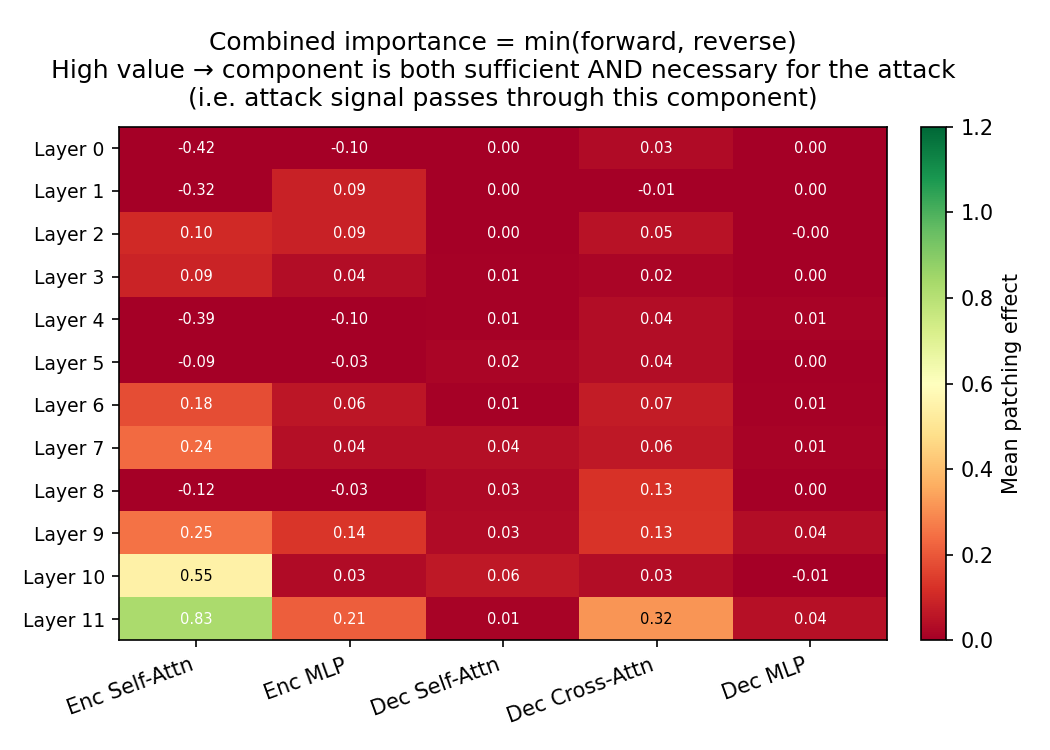
\includegraphics[width=0.17\textwidth]{outputs/attacks/important_start_5/plots/combined_layer_component_heatmap.png} \\[4pt]
\end{tabular}
\caption{Patching heatmaps for \texttt{important_start}: forward (top), reverse (middle), combined (bottom) across repetitions 1--5.}
\label{fig:hm:important_start}
\end{figure}

\begin{figure}[H]
\centering
\setlength{\tabcolsep}{2pt}
\renewcommand{\arraystretch}{0.5}
\begin{tabular}{r ccccc}
& \textbf{rep=1} & \textbf{rep=2} & \textbf{rep=3} & \textbf{rep=4} & \textbf{rep=5} \\[2pt]
\rotatebox{90}{\textbf{forward}} & 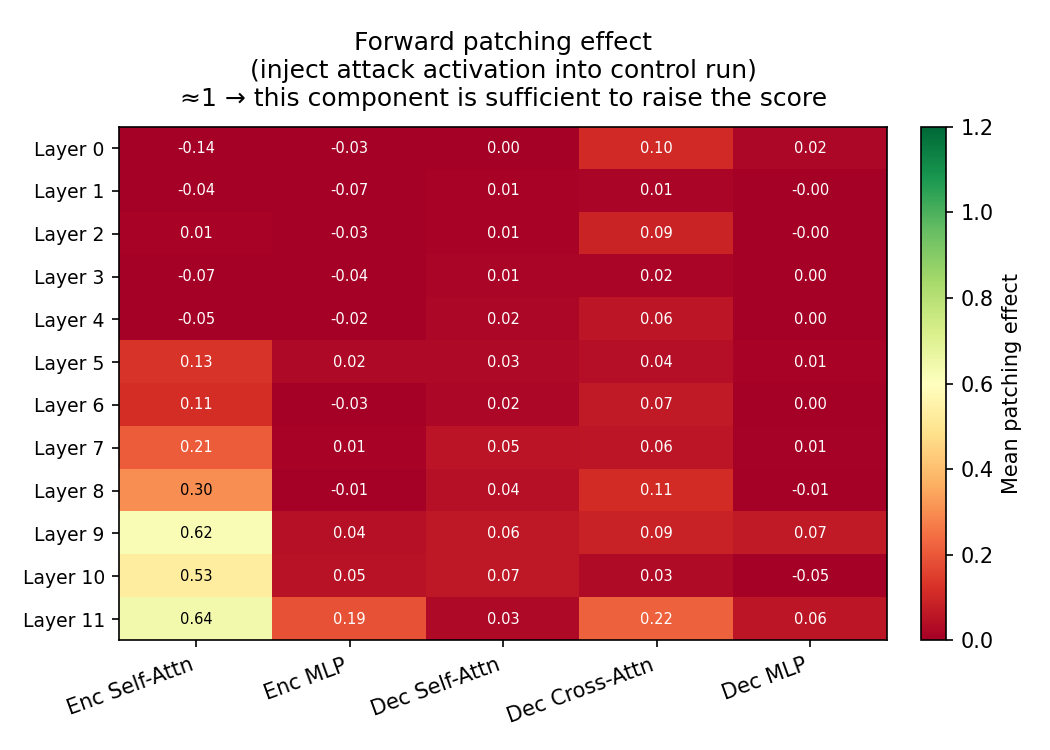
\includegraphics[width=0.17\textwidth]{outputs/attacks/information_end_1/plots/forward_layer_component_heatmap.png} & 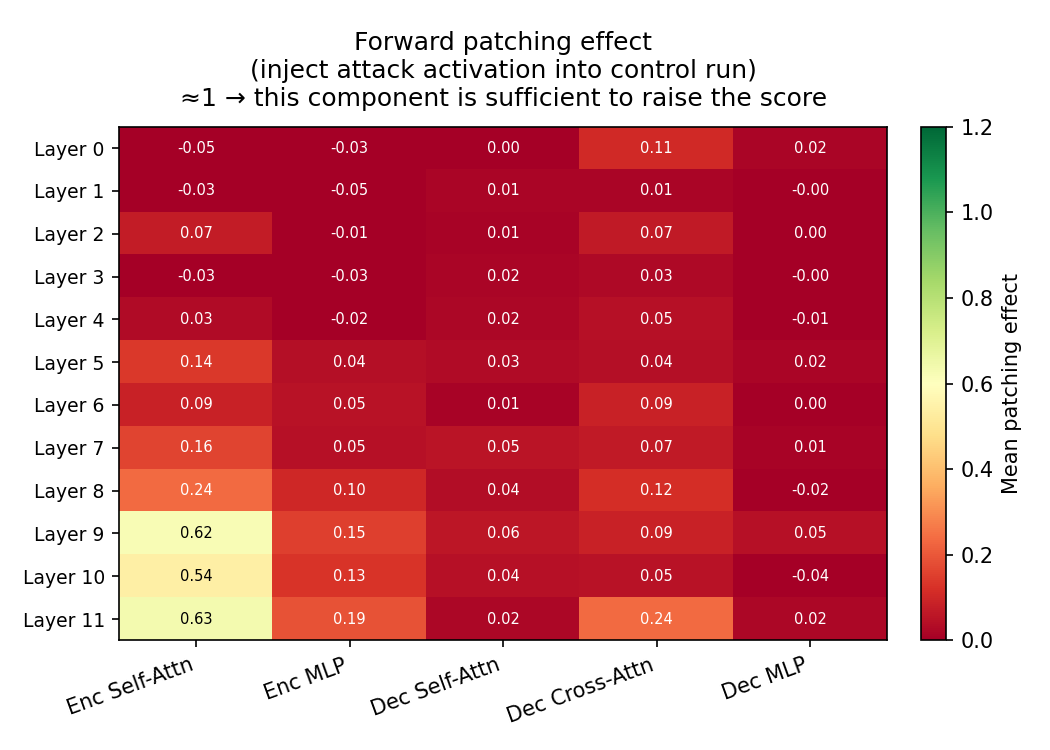
\includegraphics[width=0.17\textwidth]{outputs/attacks/information_end_2/plots/forward_layer_component_heatmap.png} & 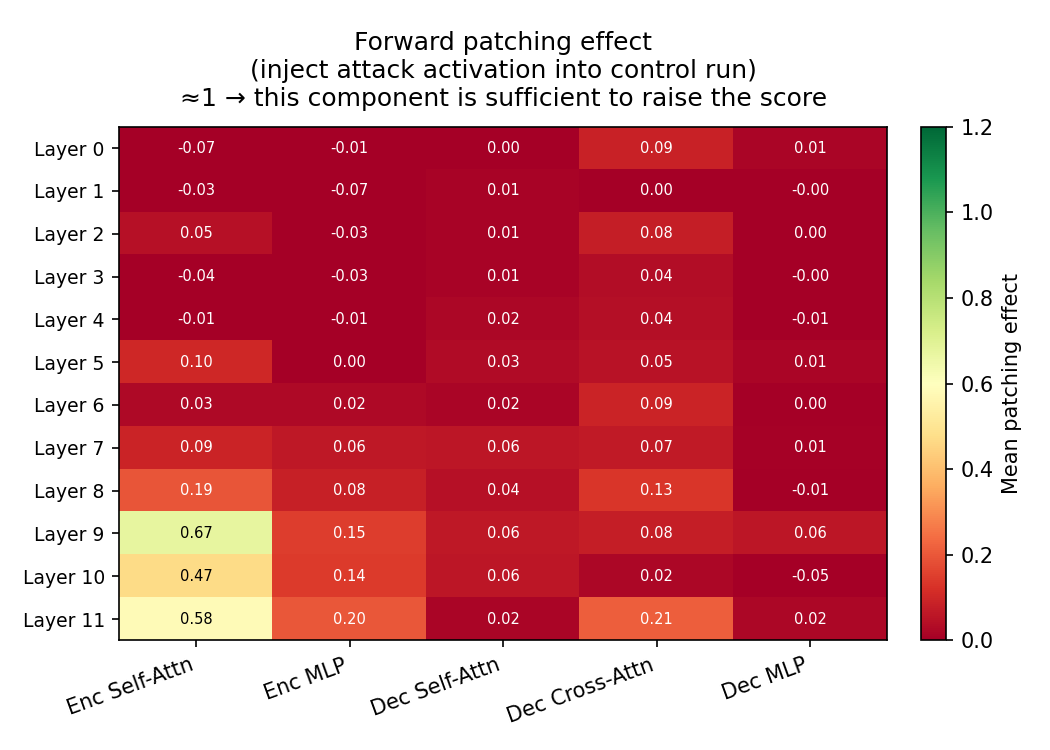
\includegraphics[width=0.17\textwidth]{outputs/attacks/information_end_3/plots/forward_layer_component_heatmap.png} & 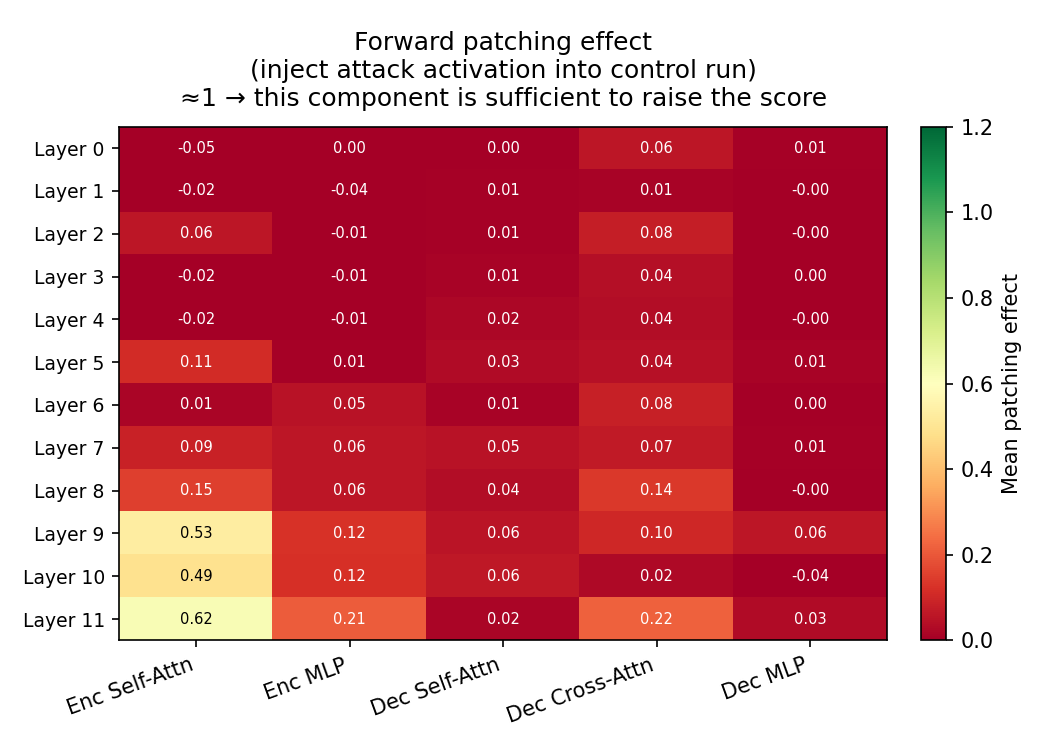
\includegraphics[width=0.17\textwidth]{outputs/attacks/information_end_4/plots/forward_layer_component_heatmap.png} & 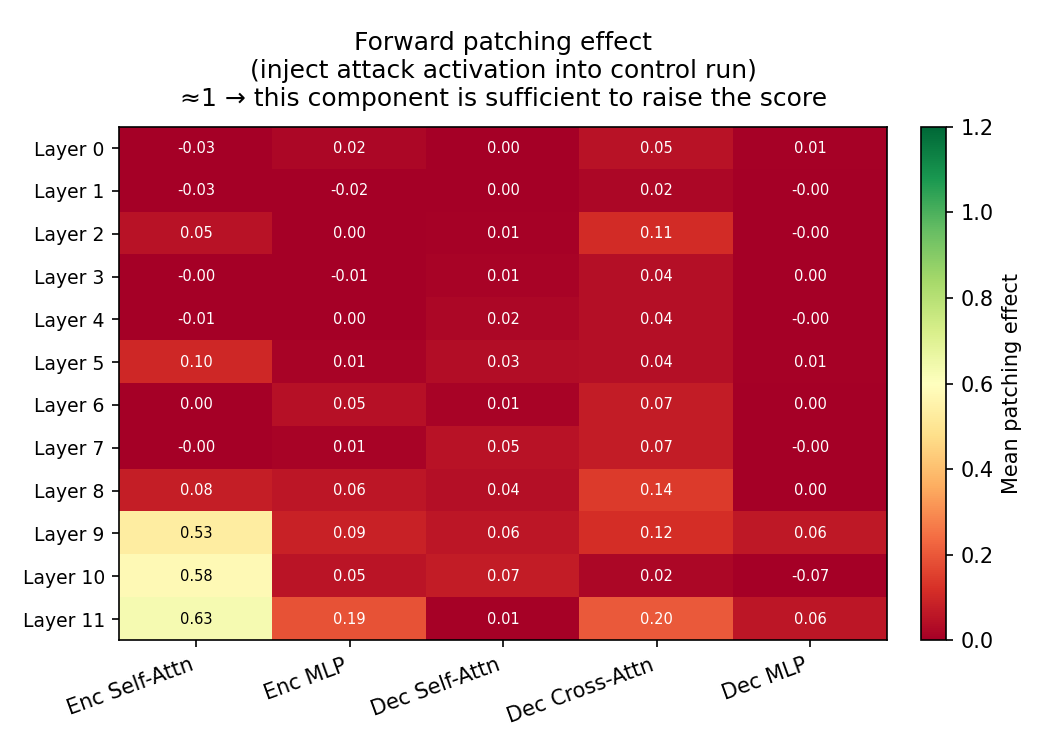
\includegraphics[width=0.17\textwidth]{outputs/attacks/information_end_5/plots/forward_layer_component_heatmap.png} \\[4pt]
\rotatebox{90}{\textbf{reverse}} & 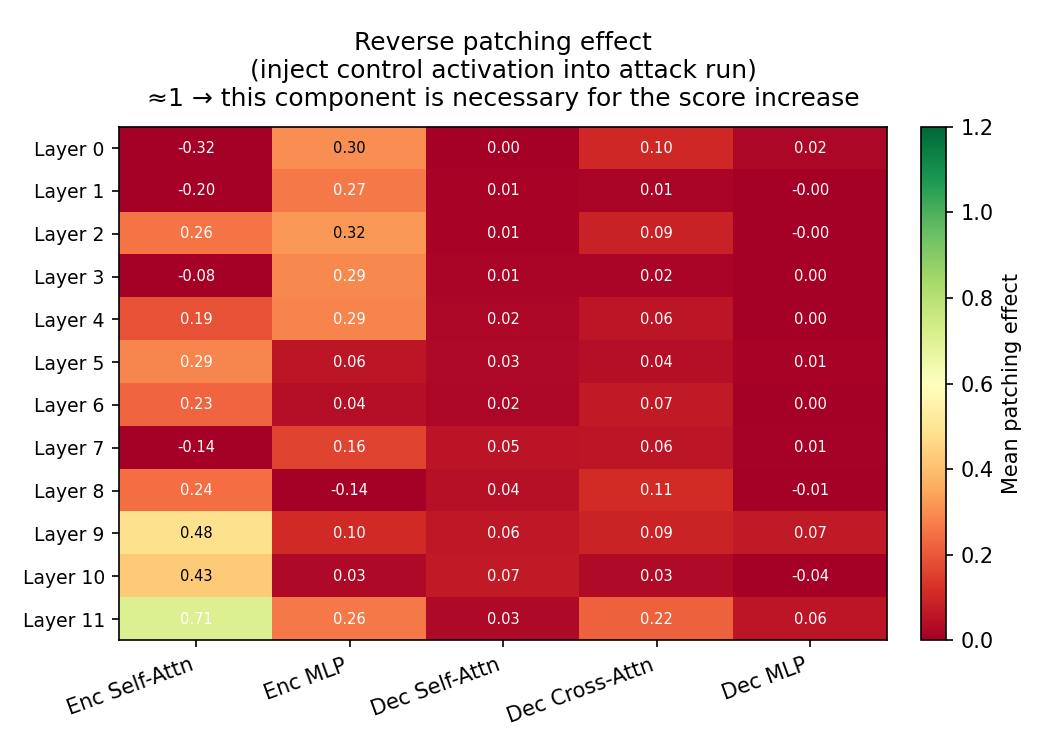
\includegraphics[width=0.17\textwidth]{outputs/attacks/information_end_1/plots/reverse_layer_component_heatmap.png} & 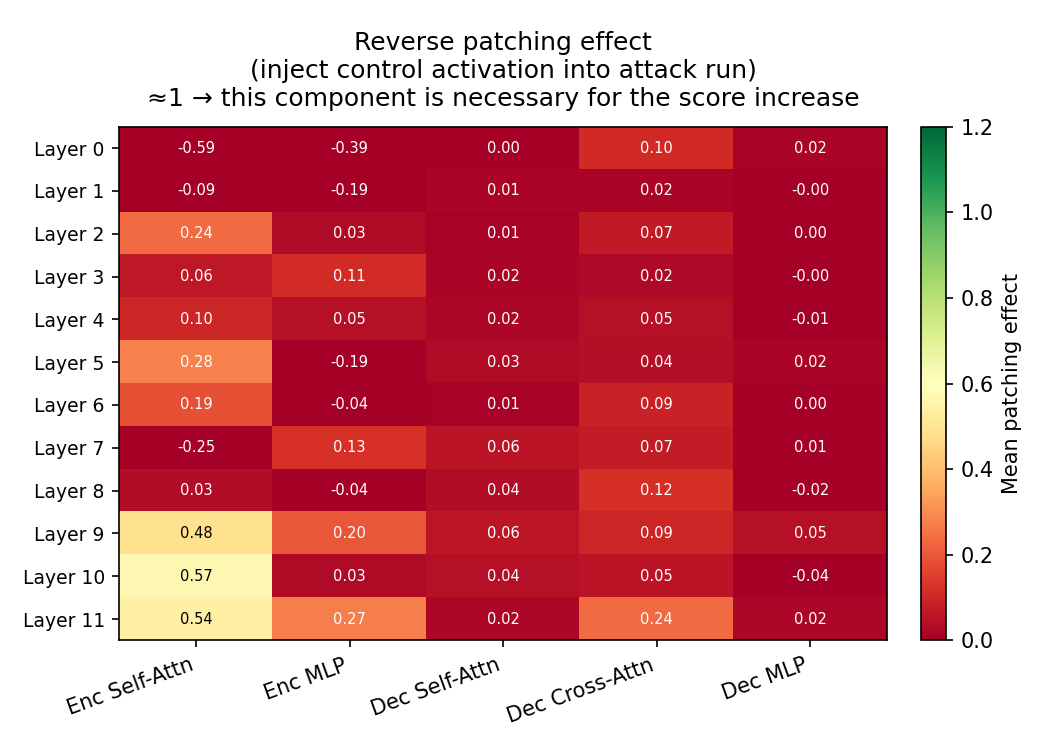
\includegraphics[width=0.17\textwidth]{outputs/attacks/information_end_2/plots/reverse_layer_component_heatmap.png} & 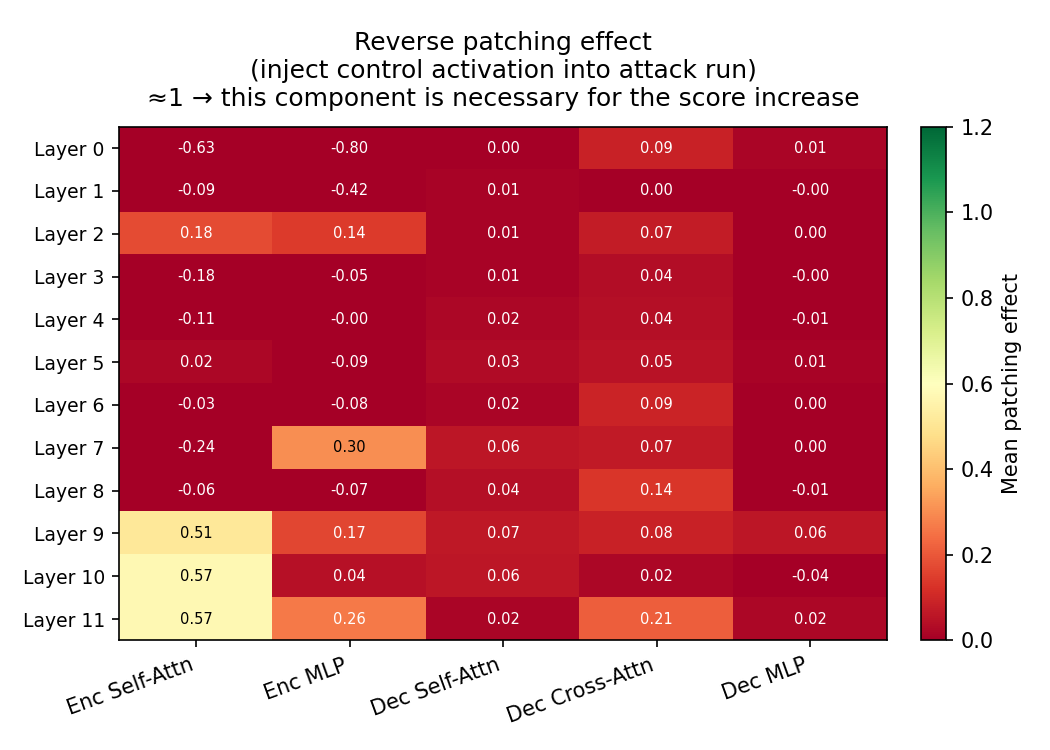
\includegraphics[width=0.17\textwidth]{outputs/attacks/information_end_3/plots/reverse_layer_component_heatmap.png} & 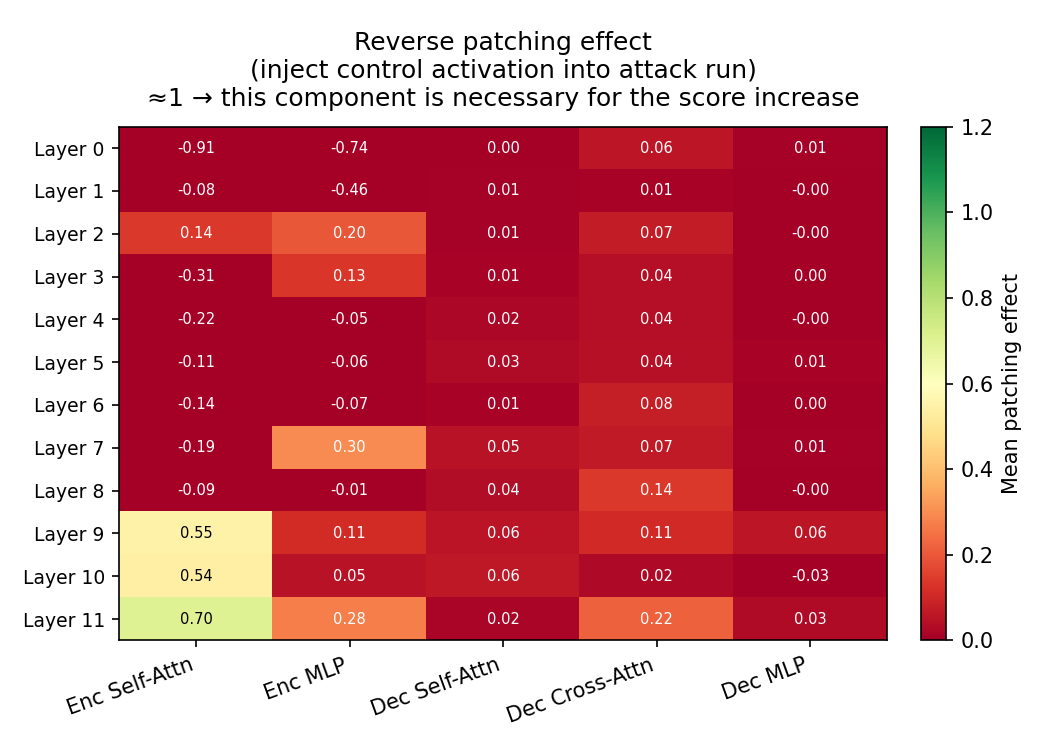
\includegraphics[width=0.17\textwidth]{outputs/attacks/information_end_4/plots/reverse_layer_component_heatmap.png} & 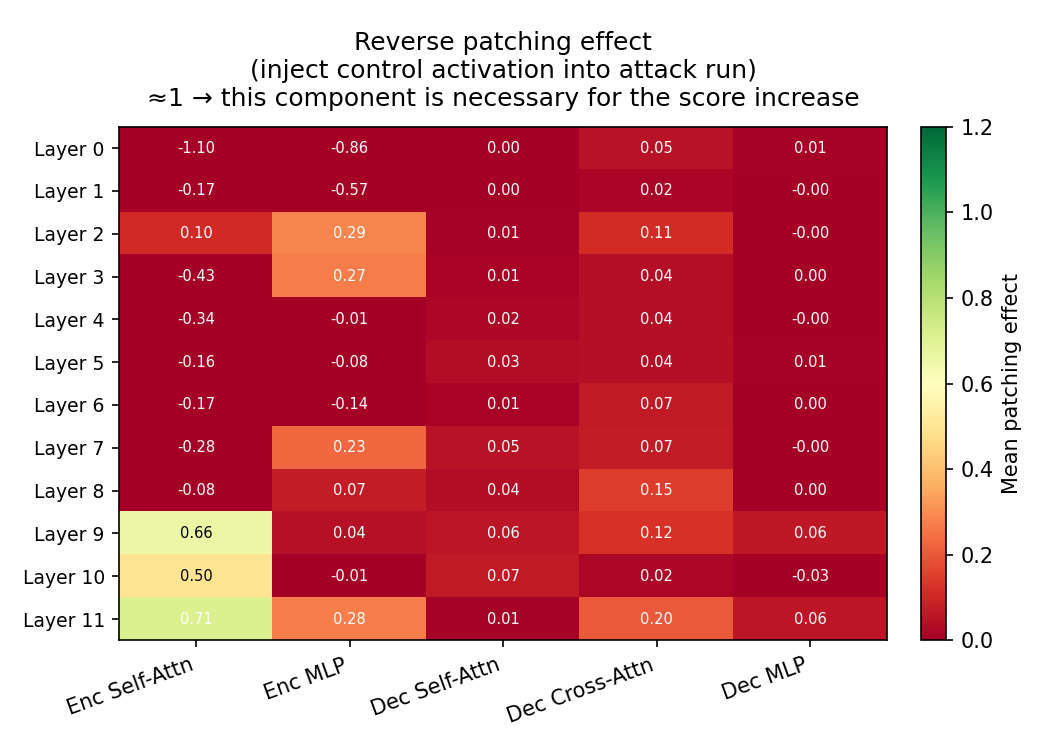
\includegraphics[width=0.17\textwidth]{outputs/attacks/information_end_5/plots/reverse_layer_component_heatmap.png} \\[4pt]
\rotatebox{90}{\textbf{combined}} & 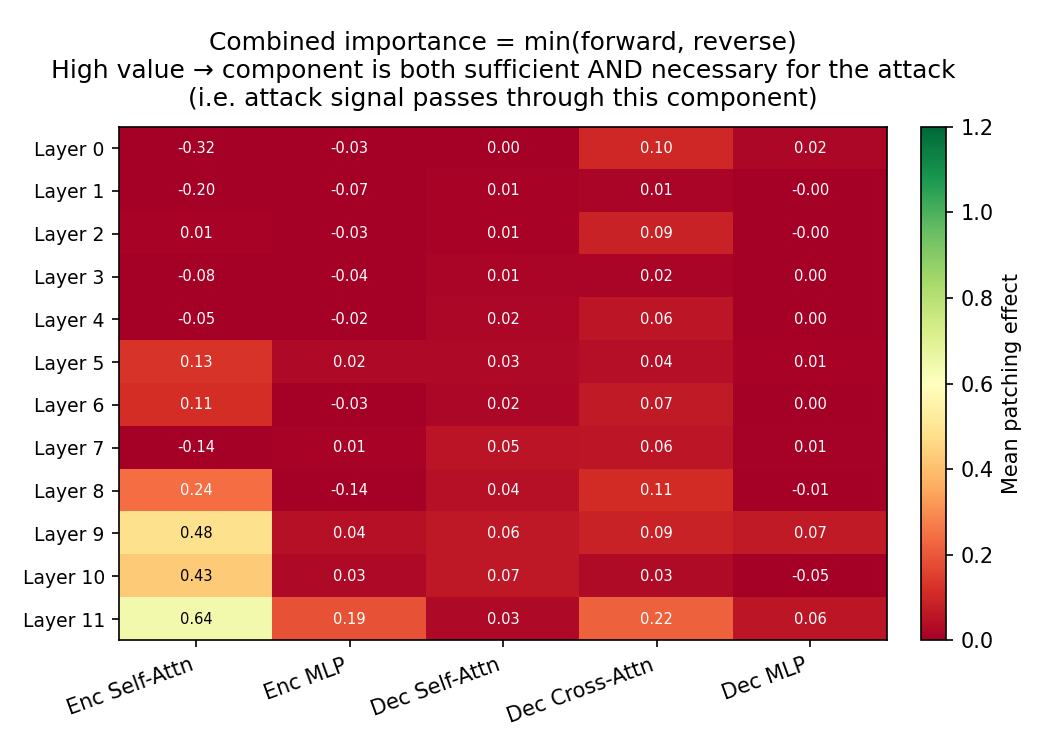
\includegraphics[width=0.17\textwidth]{outputs/attacks/information_end_1/plots/combined_layer_component_heatmap.png} & 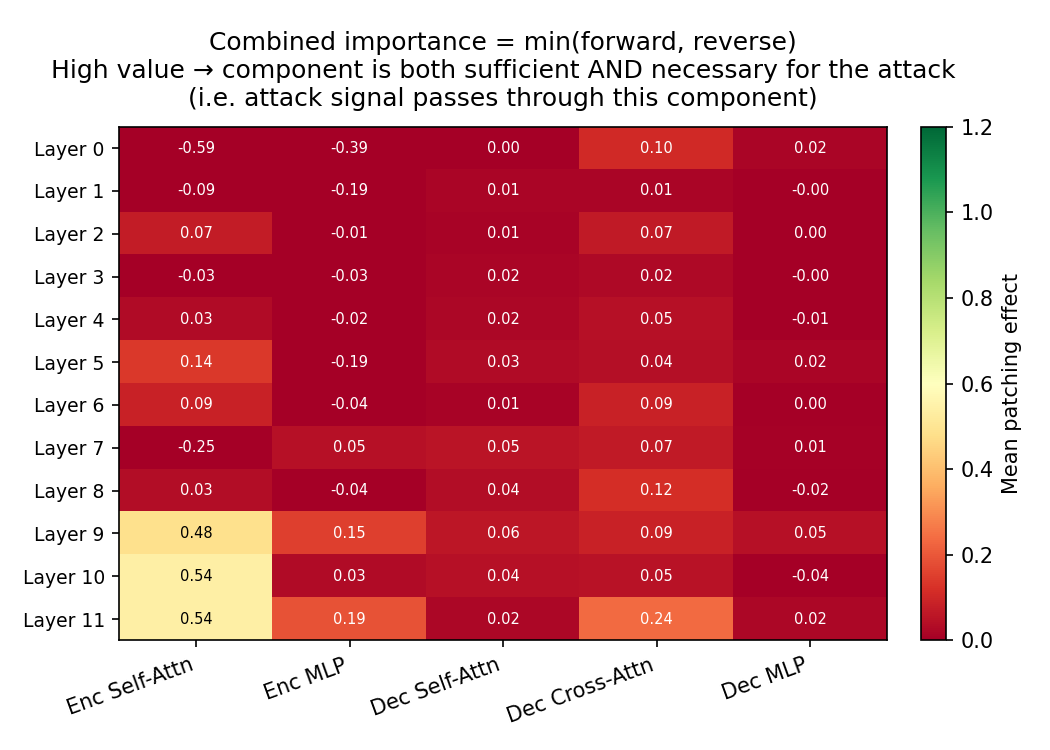
\includegraphics[width=0.17\textwidth]{outputs/attacks/information_end_2/plots/combined_layer_component_heatmap.png} & 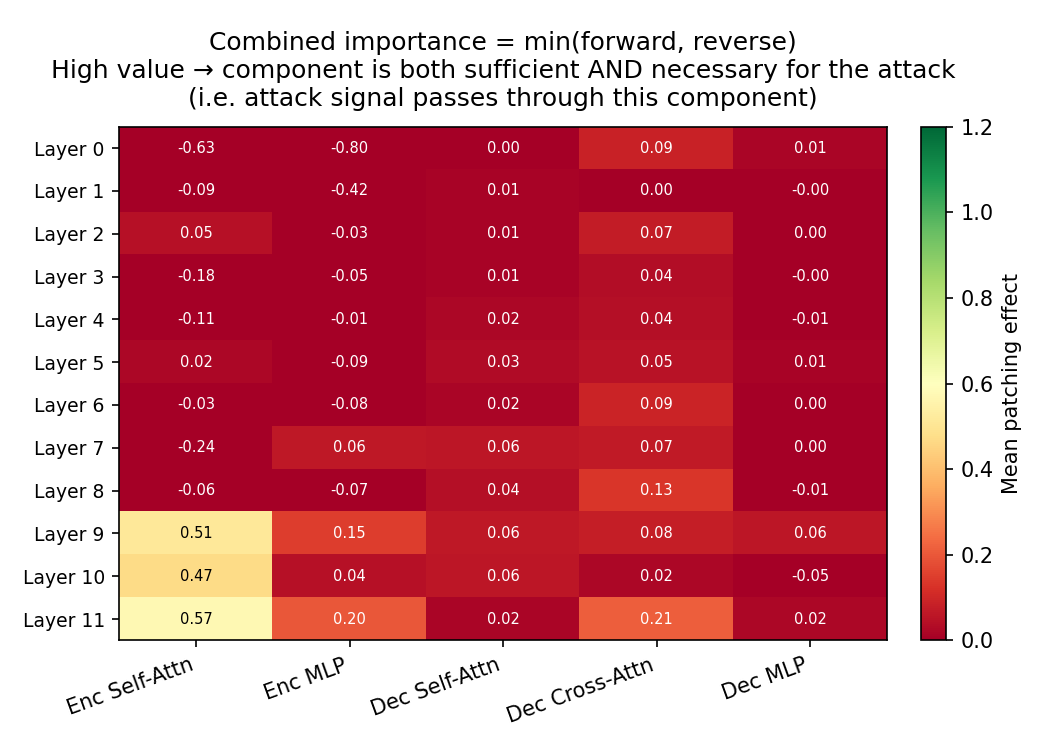
\includegraphics[width=0.17\textwidth]{outputs/attacks/information_end_3/plots/combined_layer_component_heatmap.png} & 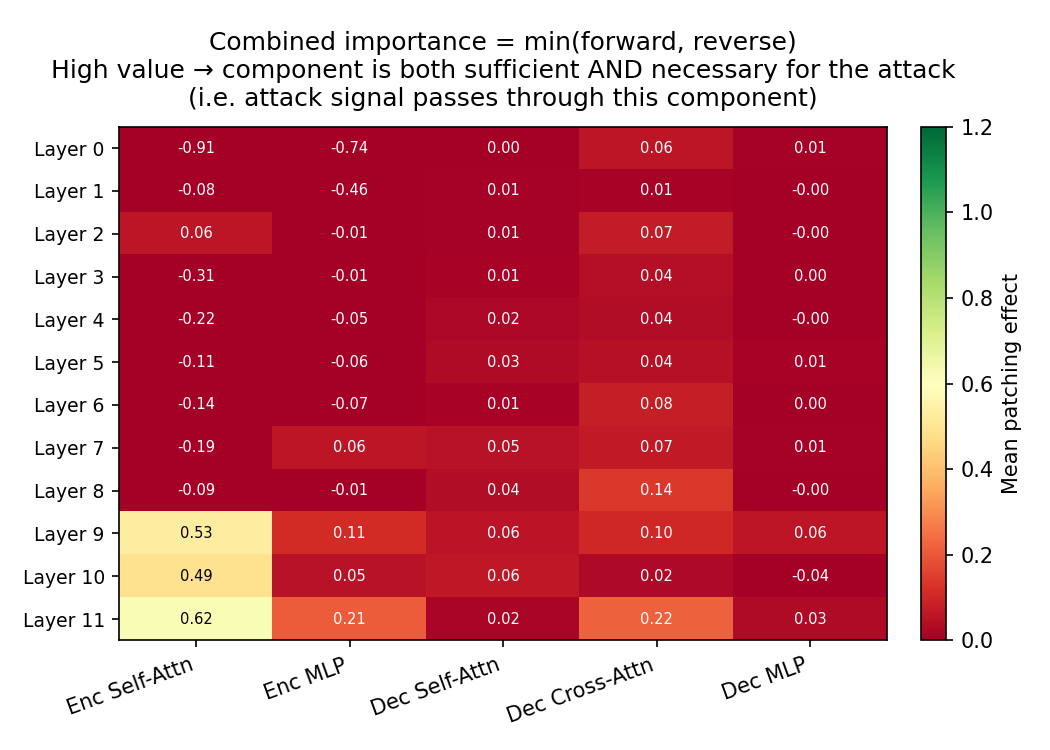
\includegraphics[width=0.17\textwidth]{outputs/attacks/information_end_4/plots/combined_layer_component_heatmap.png} & 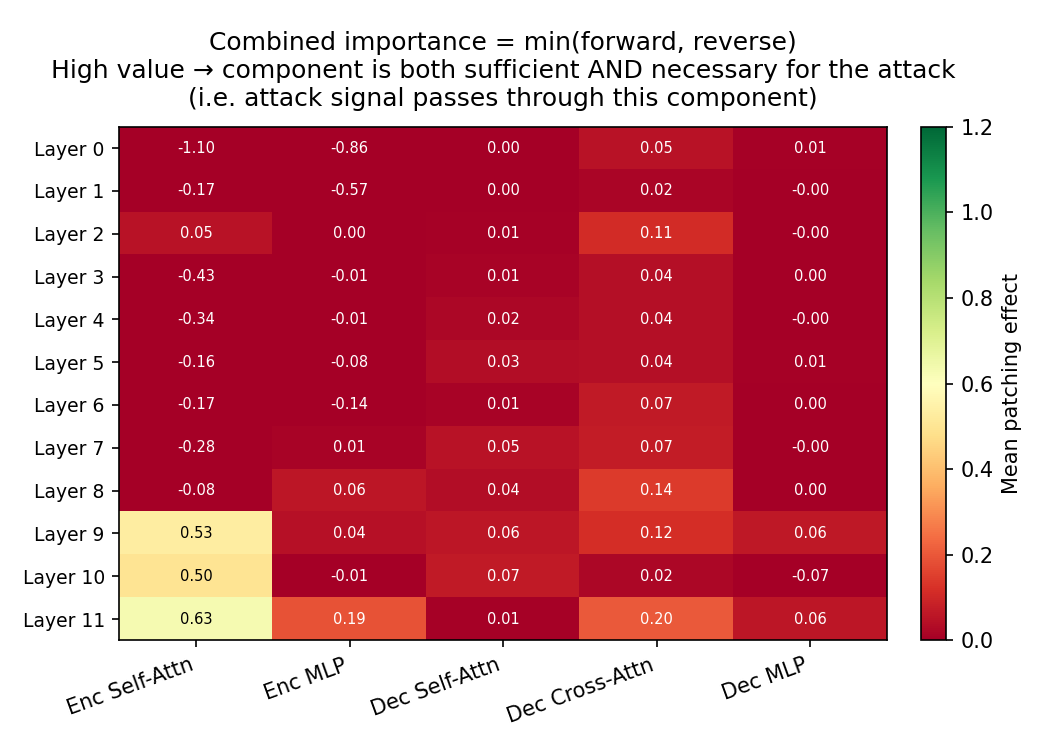
\includegraphics[width=0.17\textwidth]{outputs/attacks/information_end_5/plots/combined_layer_component_heatmap.png} \\[4pt]
\end{tabular}
\caption{Patching heatmaps for \texttt{information_end}: forward (top), reverse (middle), combined (bottom) across repetitions 1--5.}
\label{fig:hm:information_end}
\end{figure}

\begin{figure}[H]
\centering
\setlength{\tabcolsep}{2pt}
\renewcommand{\arraystretch}{0.5}
\begin{tabular}{r ccccc}
& \textbf{rep=1} & \textbf{rep=2} & \textbf{rep=3} & \textbf{rep=4} & \textbf{rep=5} \\[2pt]
\rotatebox{90}{\textbf{forward}} & 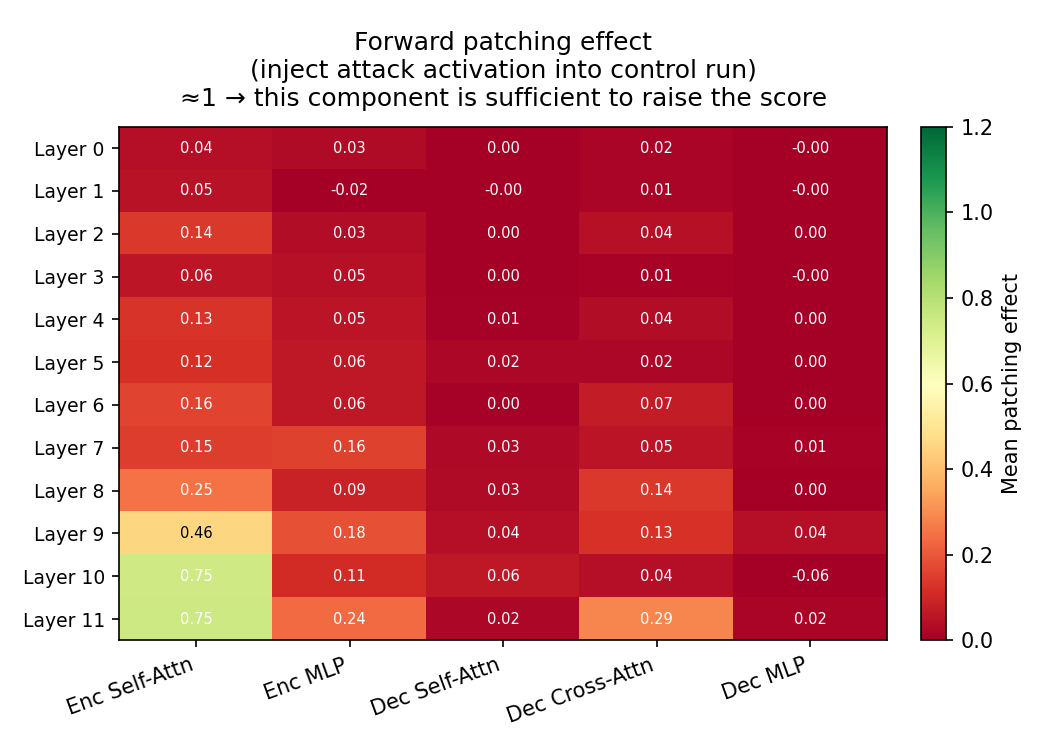
\includegraphics[width=0.17\textwidth]{outputs/attacks/information_random_1/plots/forward_layer_component_heatmap.png} & 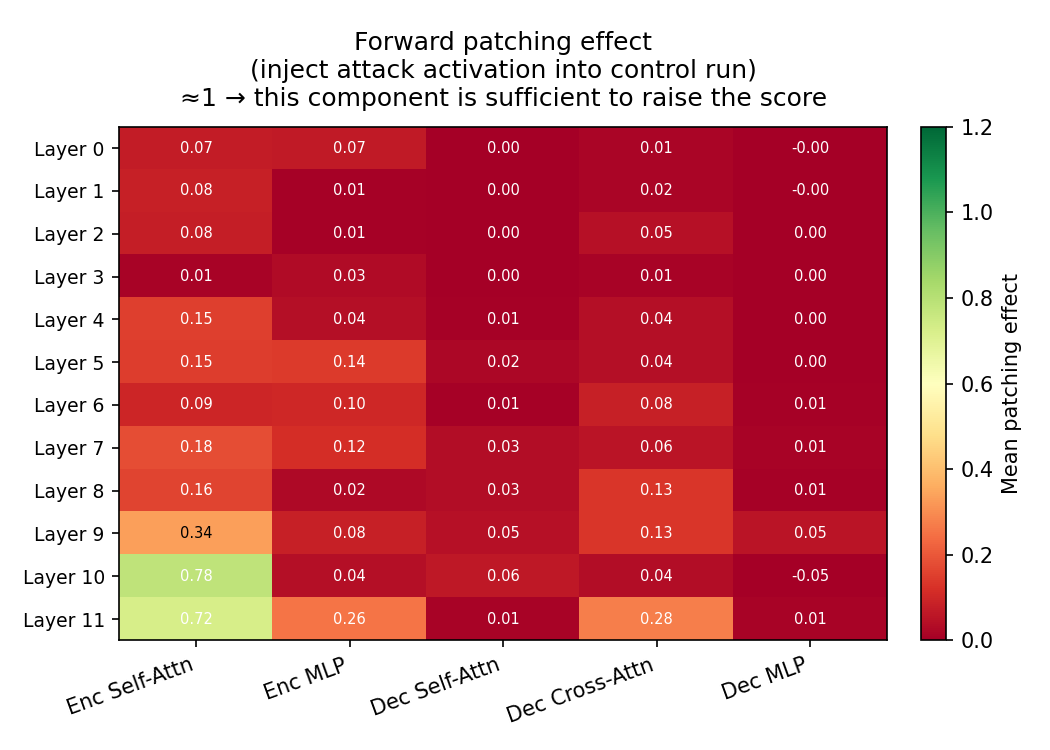
\includegraphics[width=0.17\textwidth]{outputs/attacks/information_random_2/plots/forward_layer_component_heatmap.png} & 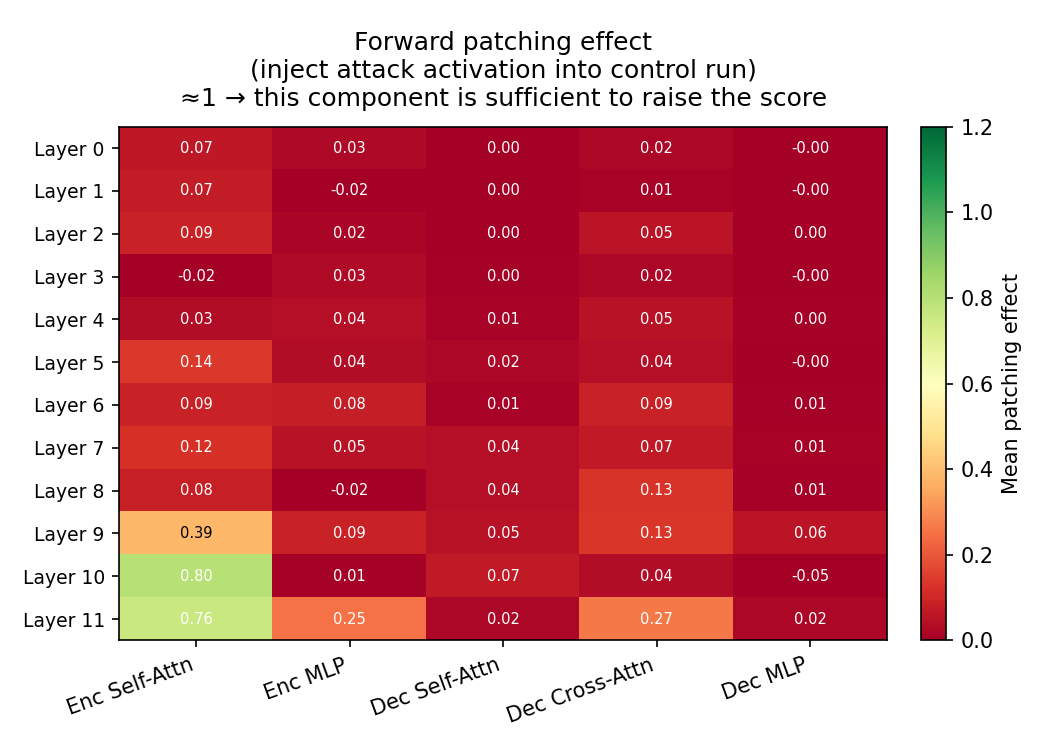
\includegraphics[width=0.17\textwidth]{outputs/attacks/information_random_3/plots/forward_layer_component_heatmap.png} & 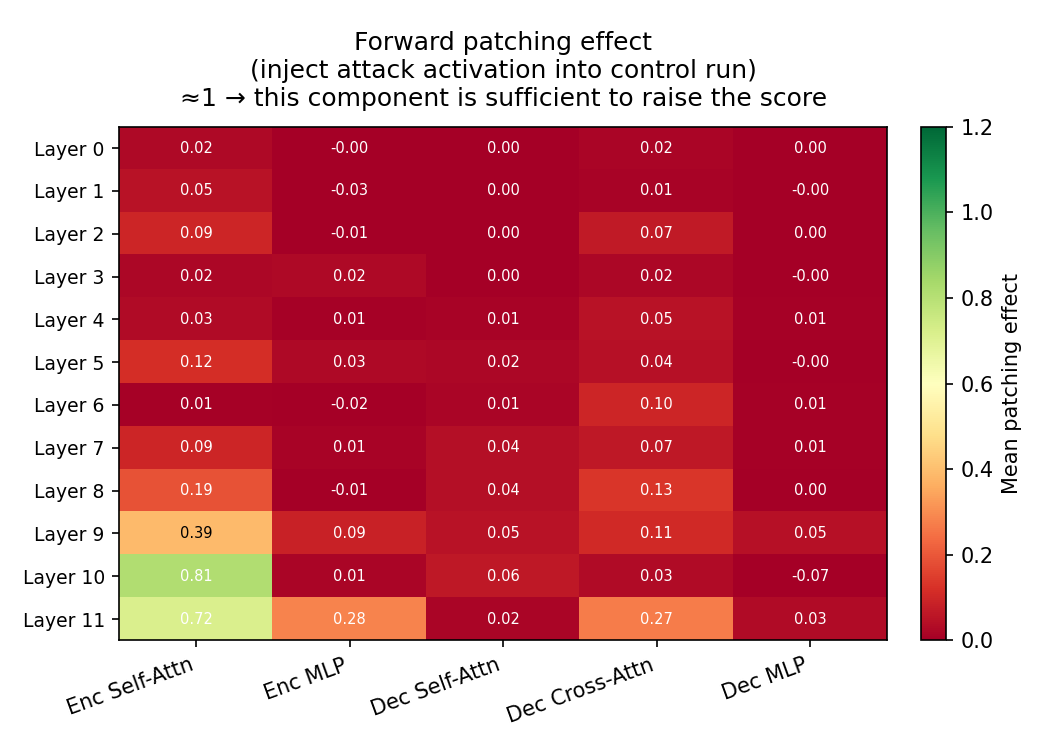
\includegraphics[width=0.17\textwidth]{outputs/attacks/information_random_4/plots/forward_layer_component_heatmap.png} & 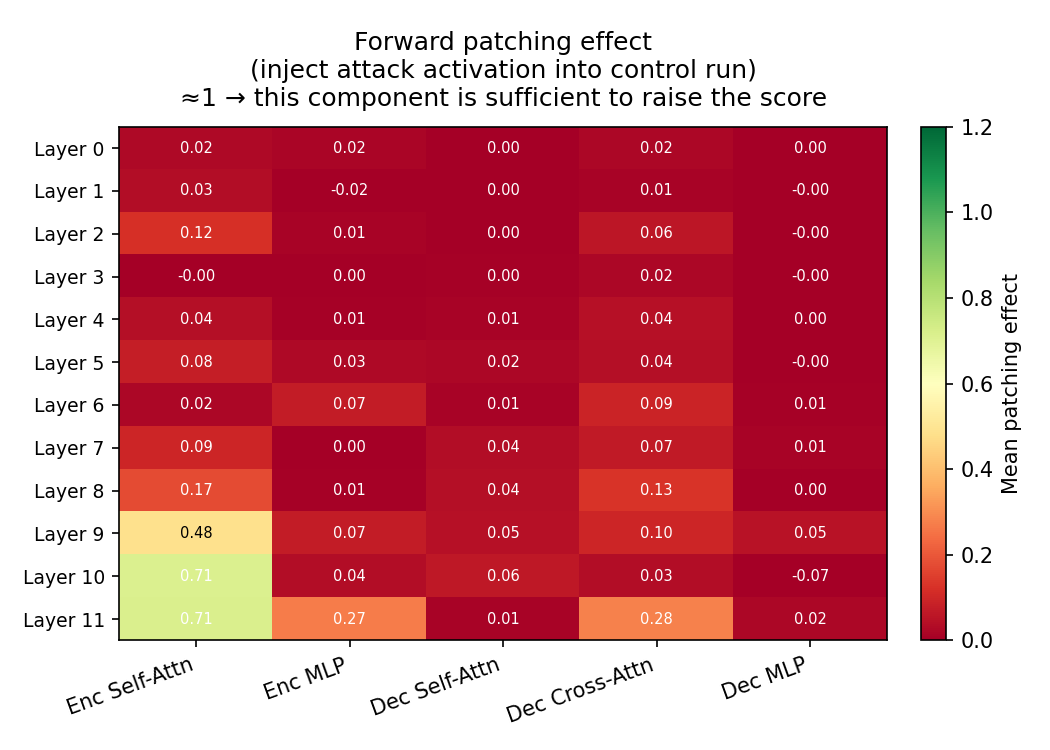
\includegraphics[width=0.17\textwidth]{outputs/attacks/information_random_5/plots/forward_layer_component_heatmap.png} \\[4pt]
\rotatebox{90}{\textbf{reverse}} & 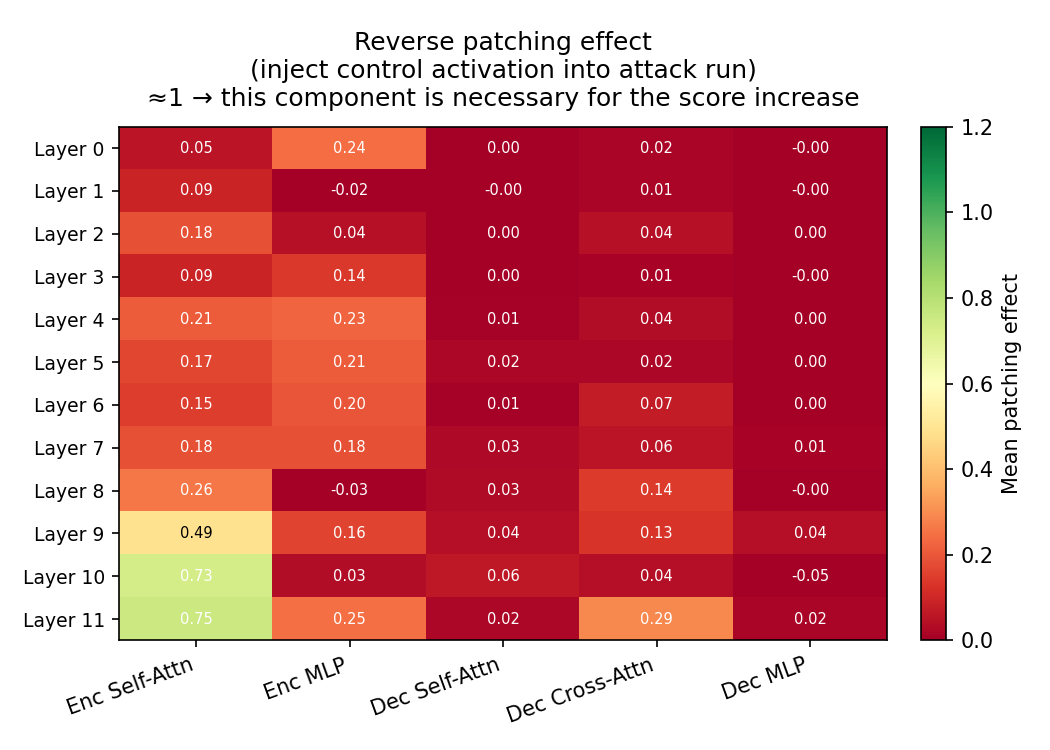
\includegraphics[width=0.17\textwidth]{outputs/attacks/information_random_1/plots/reverse_layer_component_heatmap.png} & 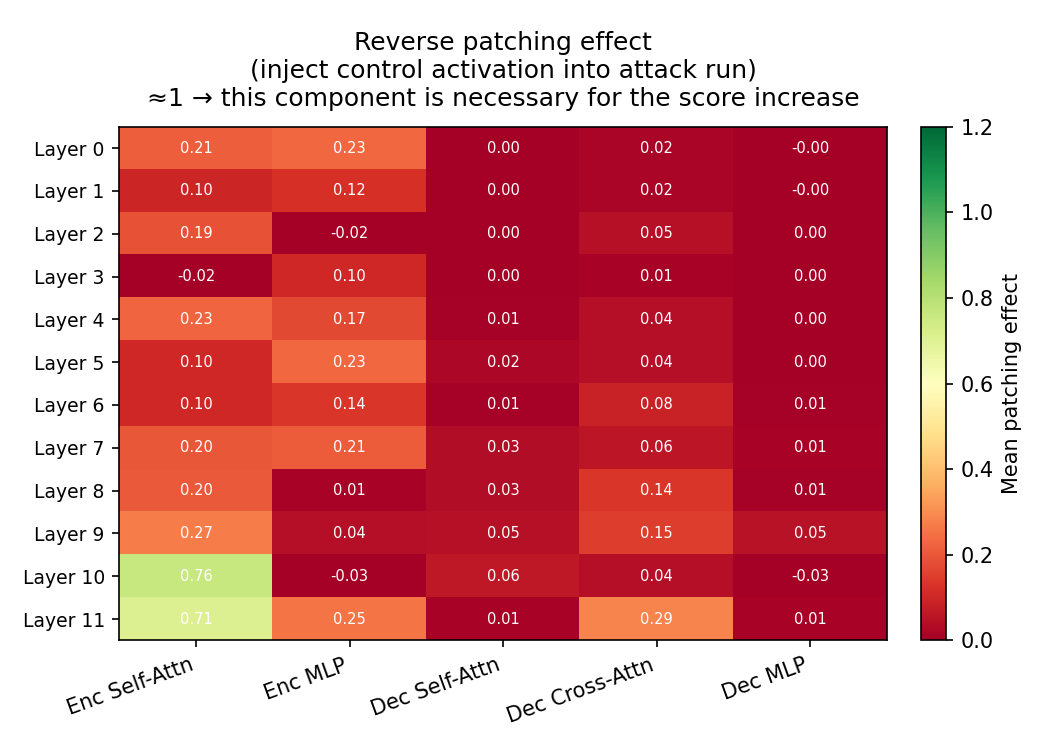
\includegraphics[width=0.17\textwidth]{outputs/attacks/information_random_2/plots/reverse_layer_component_heatmap.png} & 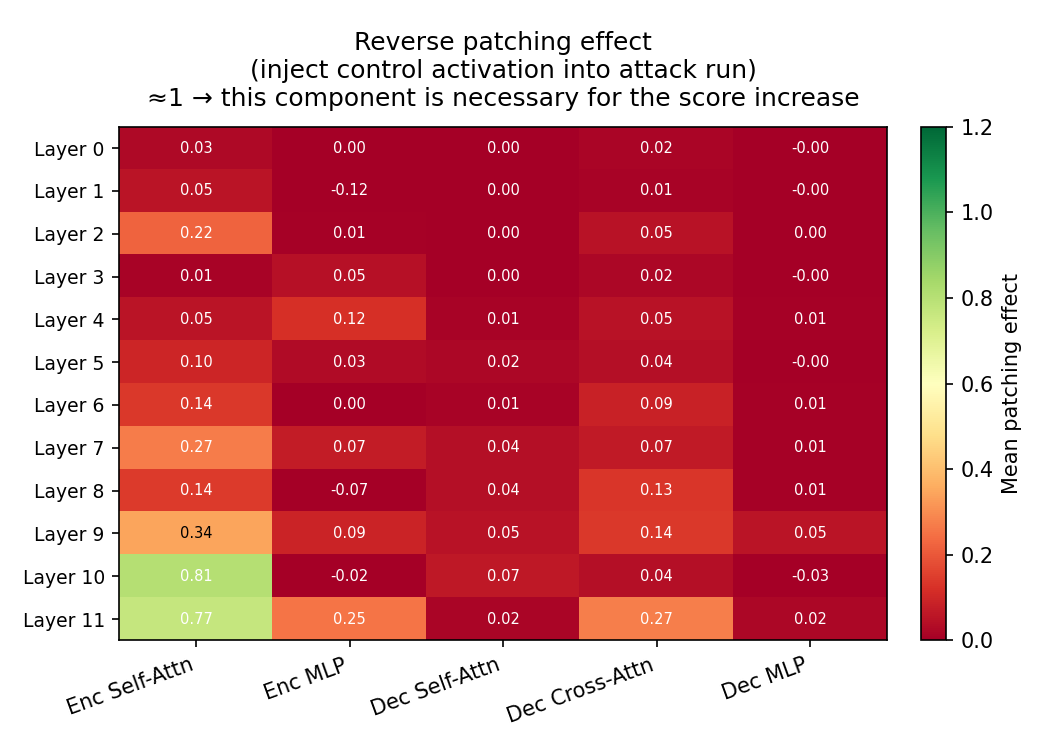
\includegraphics[width=0.17\textwidth]{outputs/attacks/information_random_3/plots/reverse_layer_component_heatmap.png} & 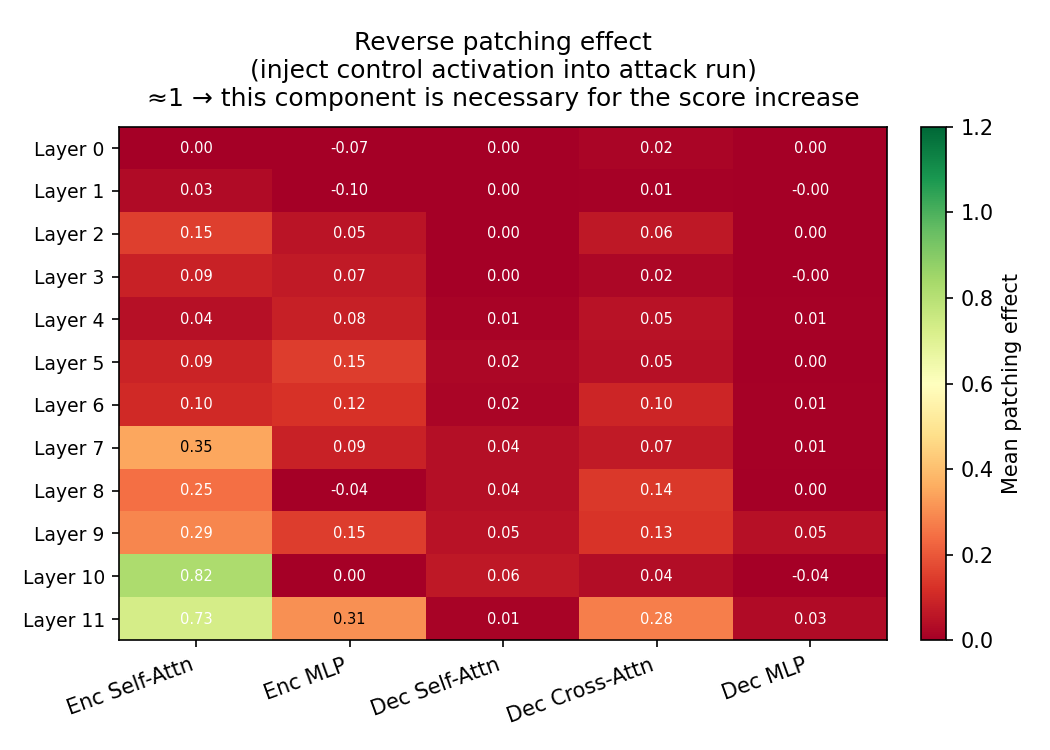
\includegraphics[width=0.17\textwidth]{outputs/attacks/information_random_4/plots/reverse_layer_component_heatmap.png} & 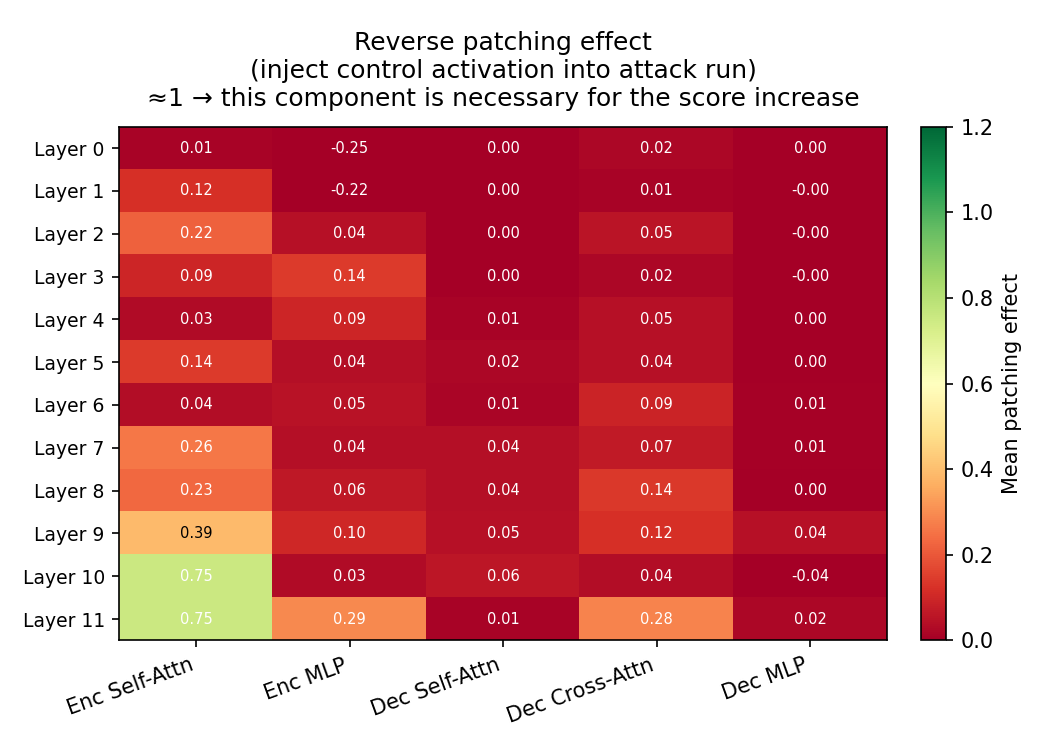
\includegraphics[width=0.17\textwidth]{outputs/attacks/information_random_5/plots/reverse_layer_component_heatmap.png} \\[4pt]
\rotatebox{90}{\textbf{combined}} & 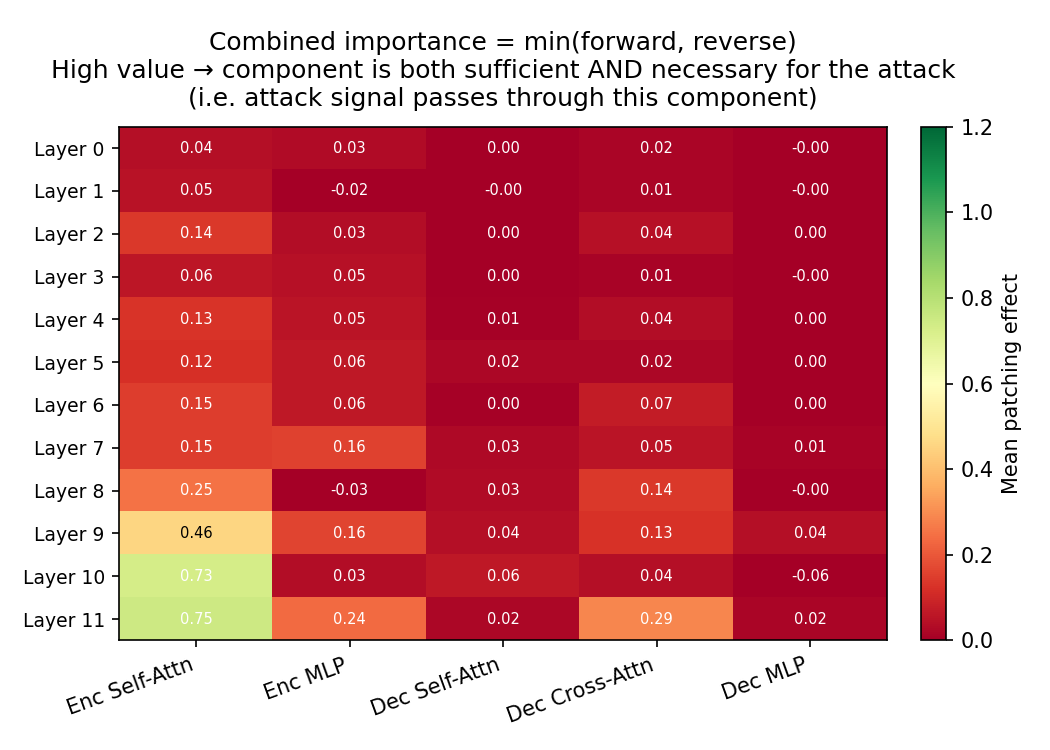
\includegraphics[width=0.17\textwidth]{outputs/attacks/information_random_1/plots/combined_layer_component_heatmap.png} & 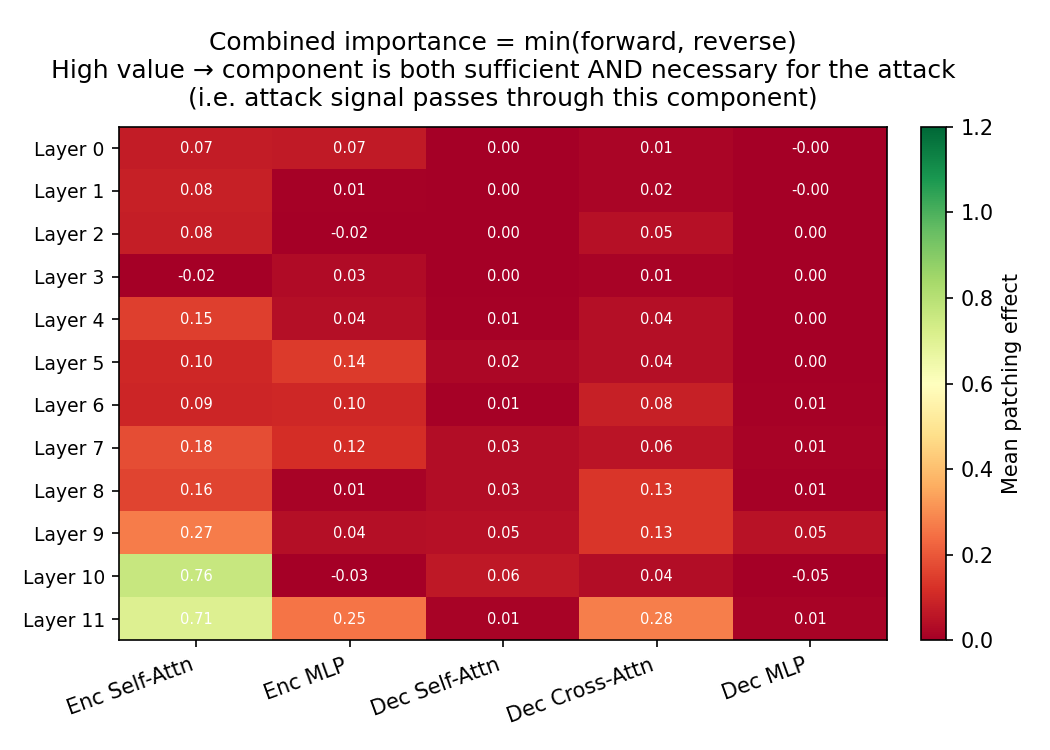
\includegraphics[width=0.17\textwidth]{outputs/attacks/information_random_2/plots/combined_layer_component_heatmap.png} & 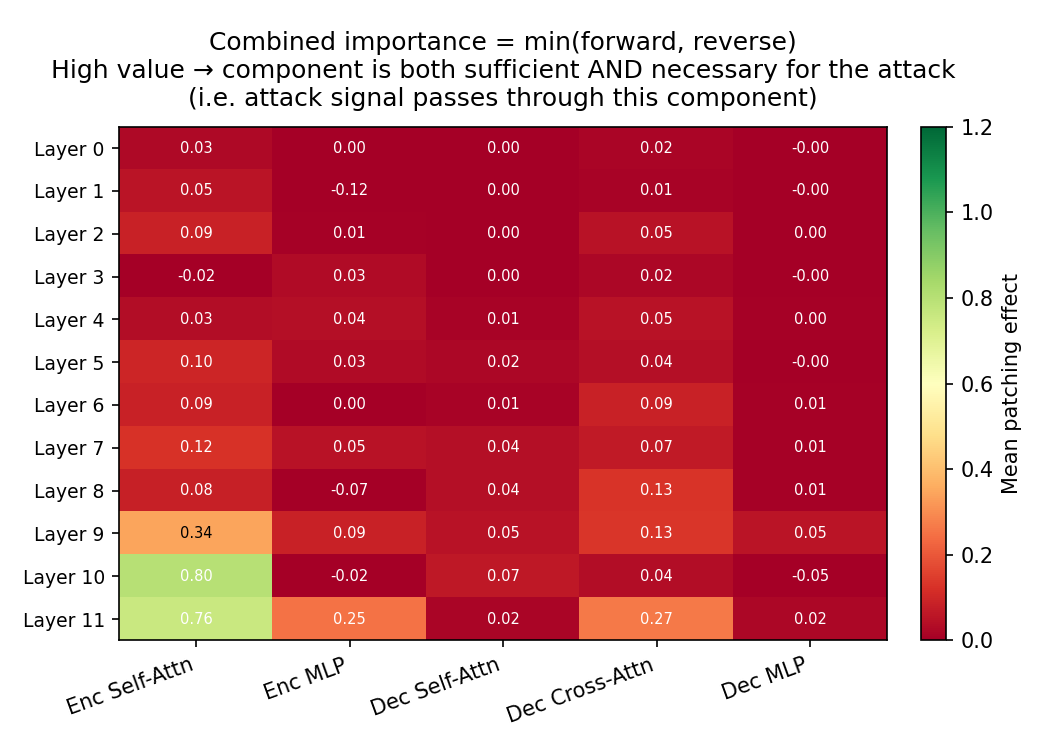
\includegraphics[width=0.17\textwidth]{outputs/attacks/information_random_3/plots/combined_layer_component_heatmap.png} & 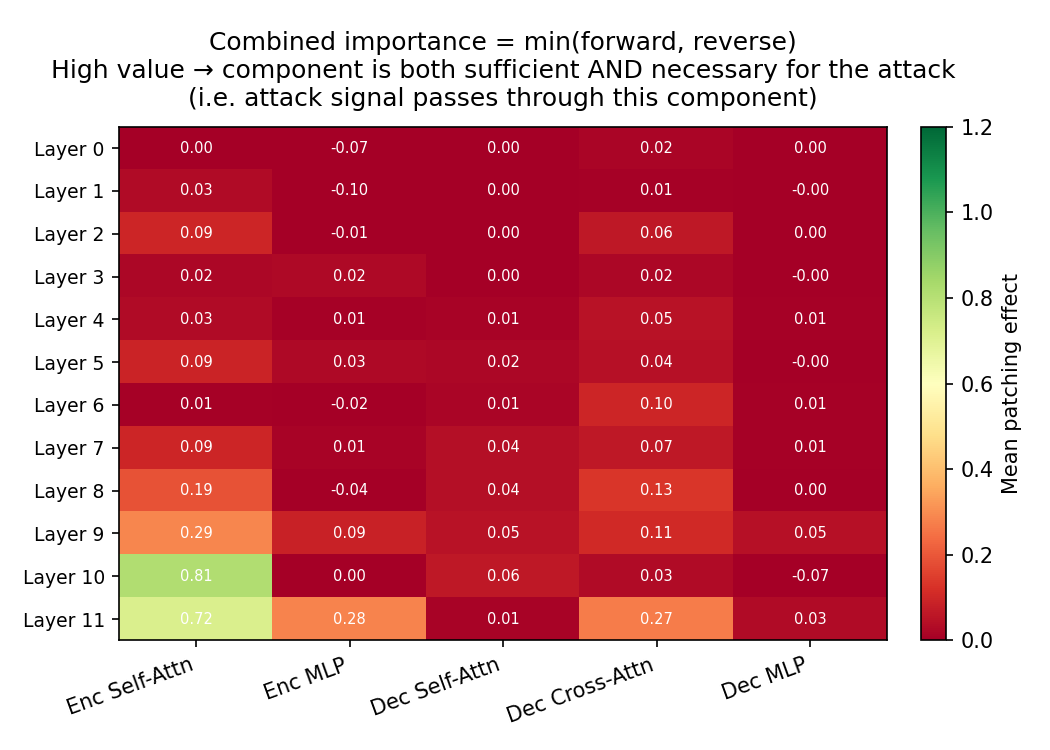
\includegraphics[width=0.17\textwidth]{outputs/attacks/information_random_4/plots/combined_layer_component_heatmap.png} & 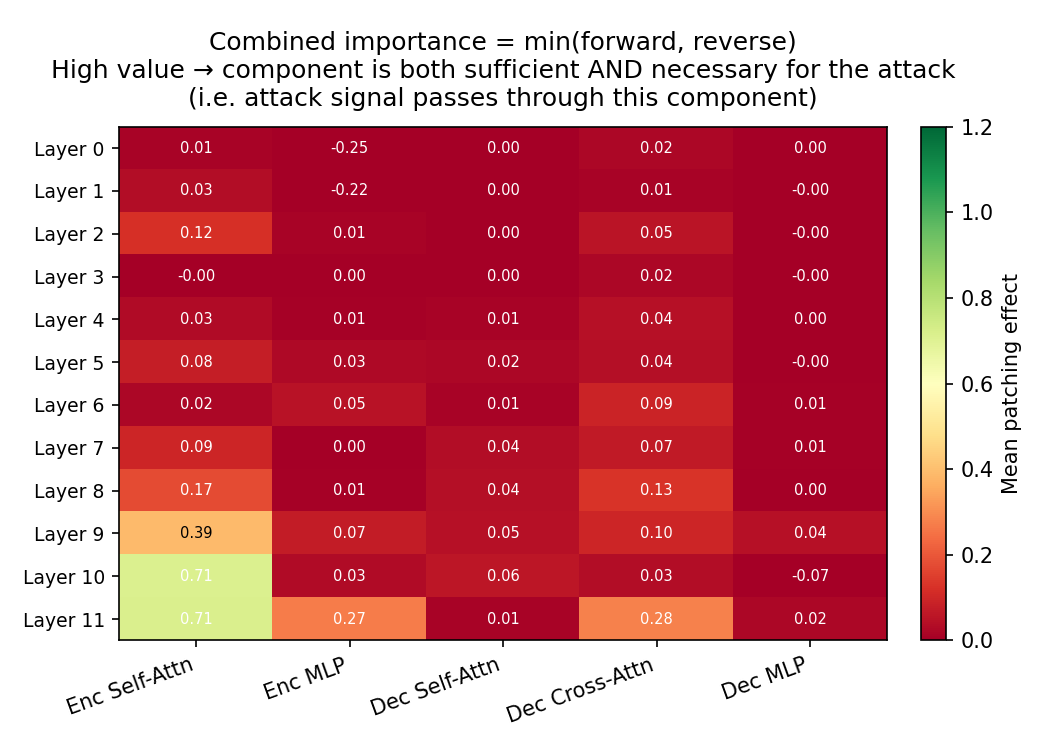
\includegraphics[width=0.17\textwidth]{outputs/attacks/information_random_5/plots/combined_layer_component_heatmap.png} \\[4pt]
\end{tabular}
\caption{Patching heatmaps for \texttt{information_random}: forward (top), reverse (middle), combined (bottom) across repetitions 1--5.}
\label{fig:hm:information_random}
\end{figure}

\begin{figure}[H]
\centering
\setlength{\tabcolsep}{2pt}
\renewcommand{\arraystretch}{0.5}
\begin{tabular}{r ccccc}
& \textbf{rep=1} & \textbf{rep=2} & \textbf{rep=3} & \textbf{rep=4} & \textbf{rep=5} \\[2pt]
\rotatebox{90}{\textbf{forward}} & 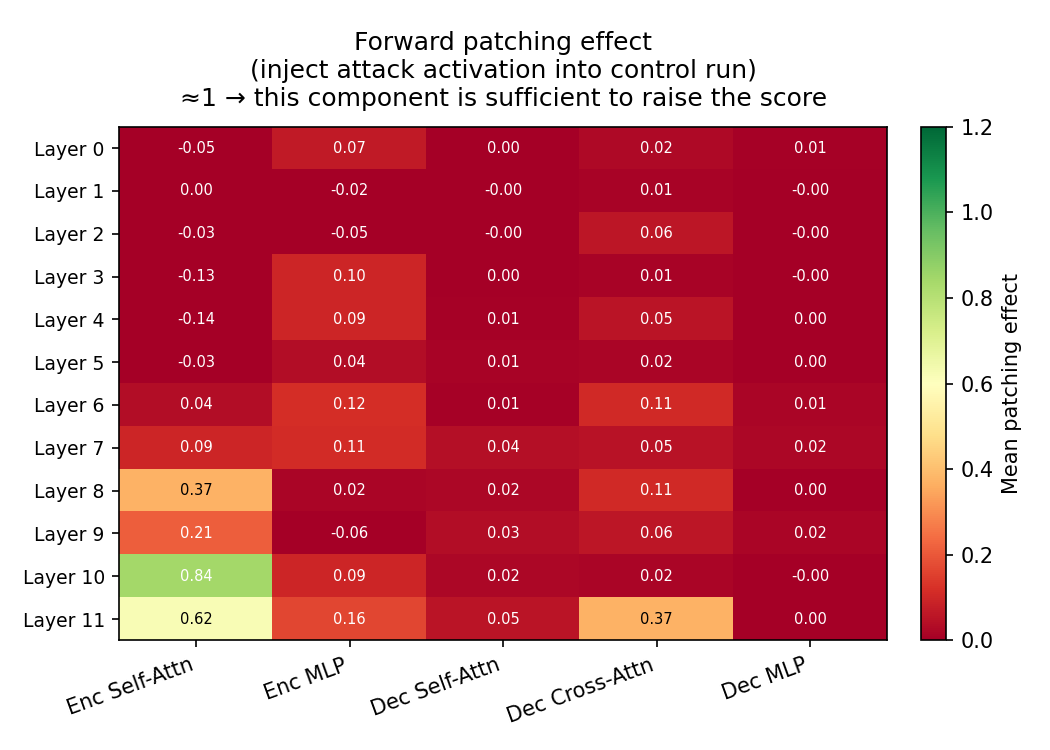
\includegraphics[width=0.17\textwidth]{outputs/attacks/information_start_1/plots/forward_layer_component_heatmap.png} & 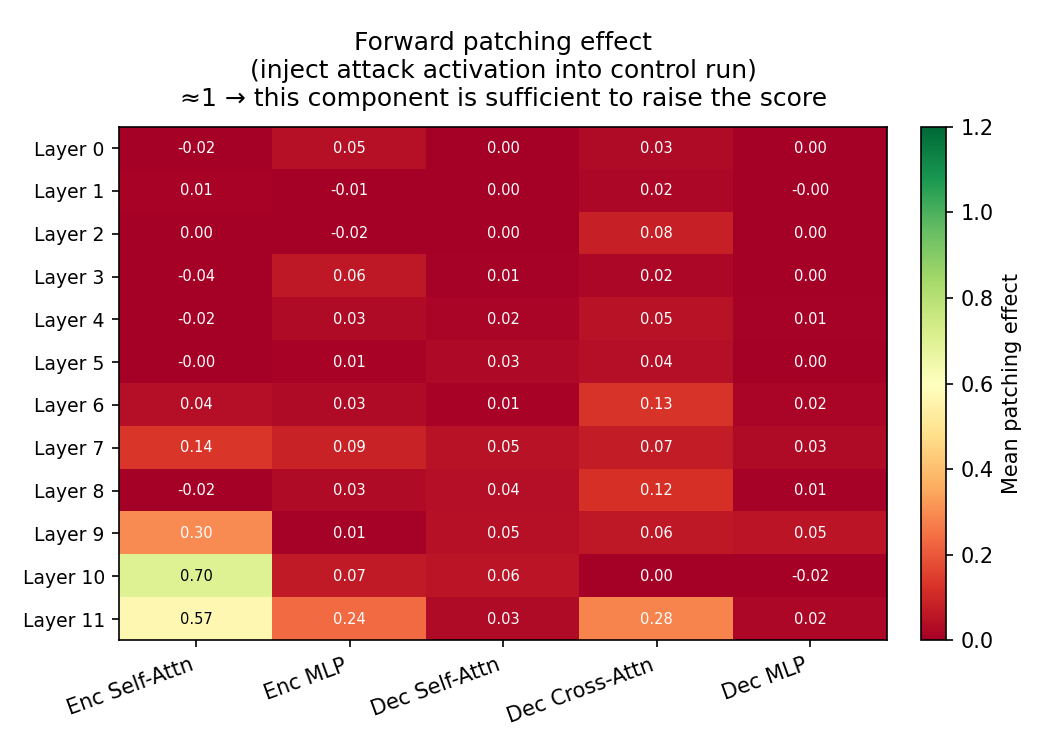
\includegraphics[width=0.17\textwidth]{outputs/attacks/information_start_2/plots/forward_layer_component_heatmap.png} & 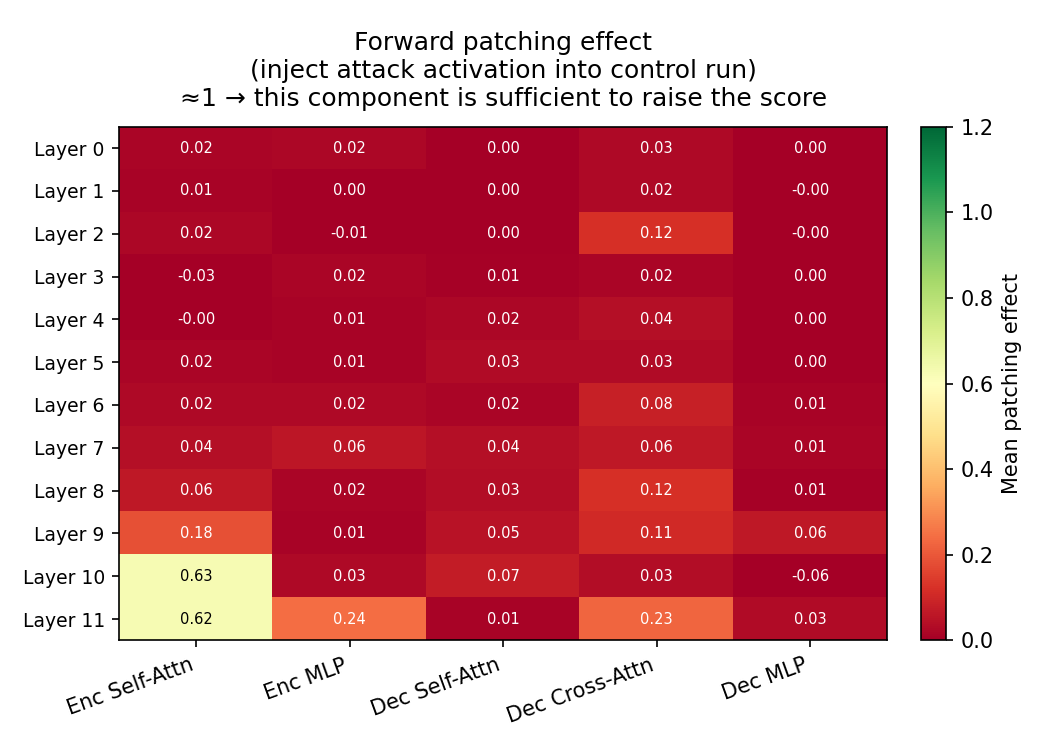
\includegraphics[width=0.17\textwidth]{outputs/attacks/information_start_3/plots/forward_layer_component_heatmap.png} & 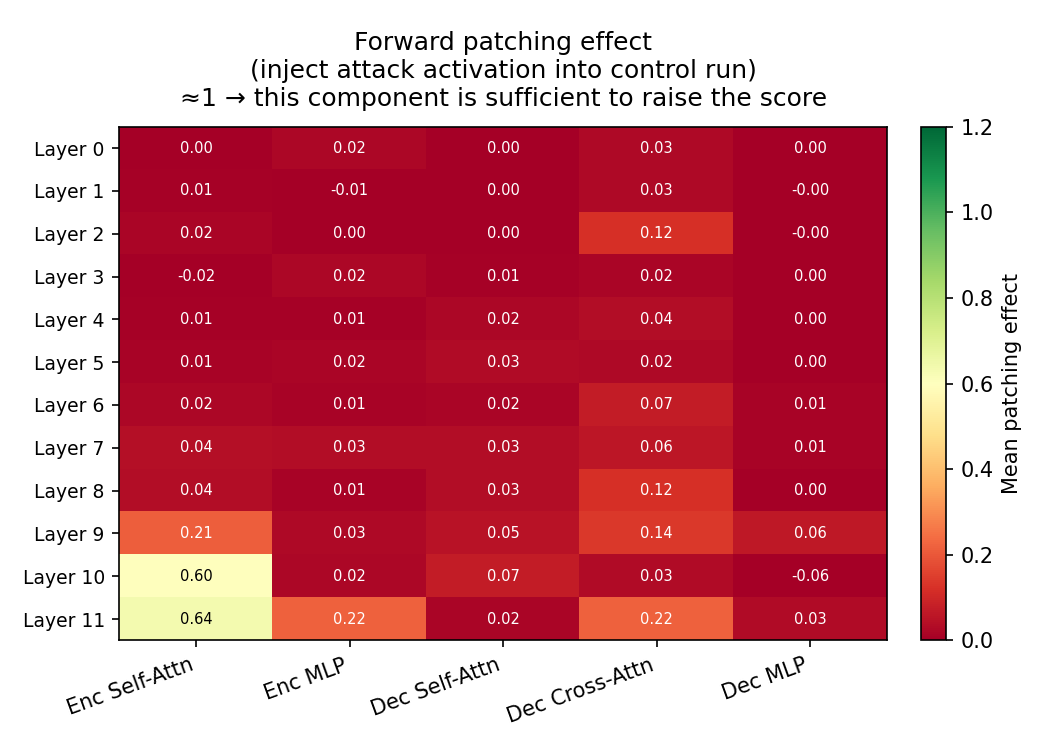
\includegraphics[width=0.17\textwidth]{outputs/attacks/information_start_4/plots/forward_layer_component_heatmap.png} & 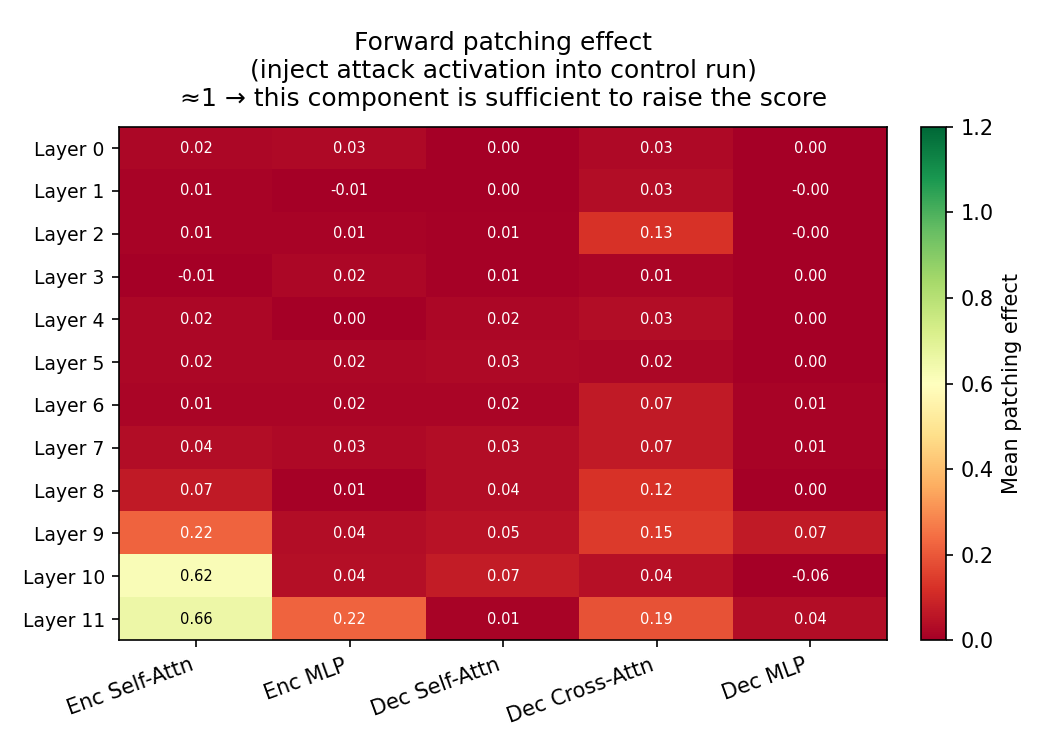
\includegraphics[width=0.17\textwidth]{outputs/attacks/information_start_5/plots/forward_layer_component_heatmap.png} \\[4pt]
\rotatebox{90}{\textbf{reverse}} & 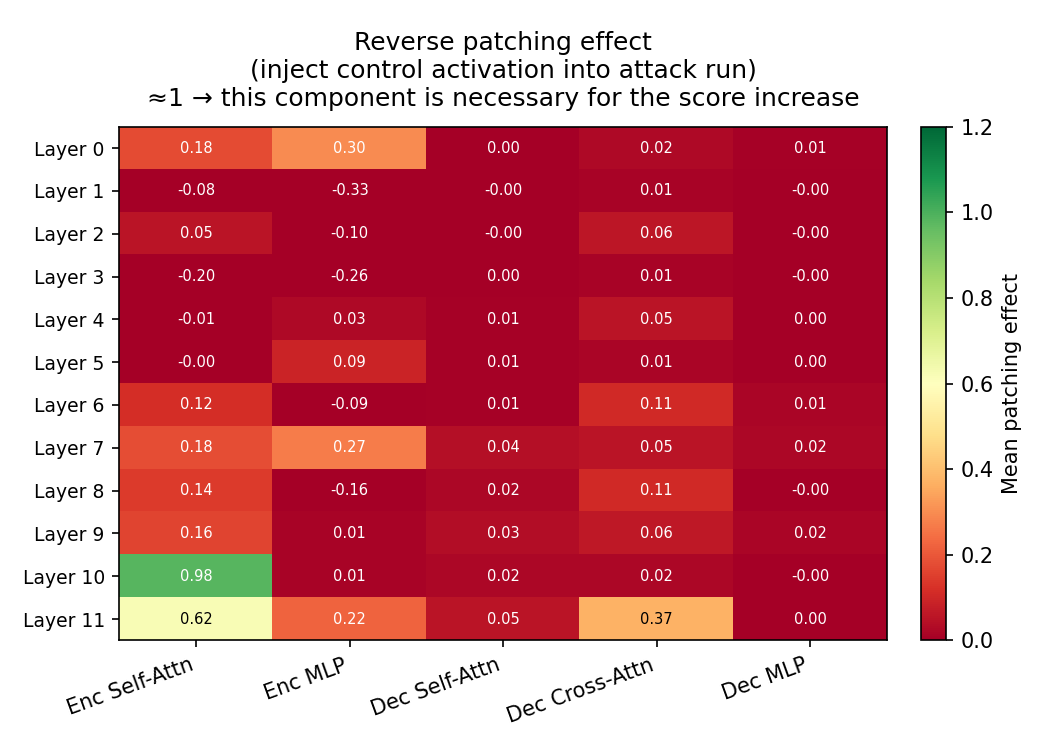
\includegraphics[width=0.17\textwidth]{outputs/attacks/information_start_1/plots/reverse_layer_component_heatmap.png} & 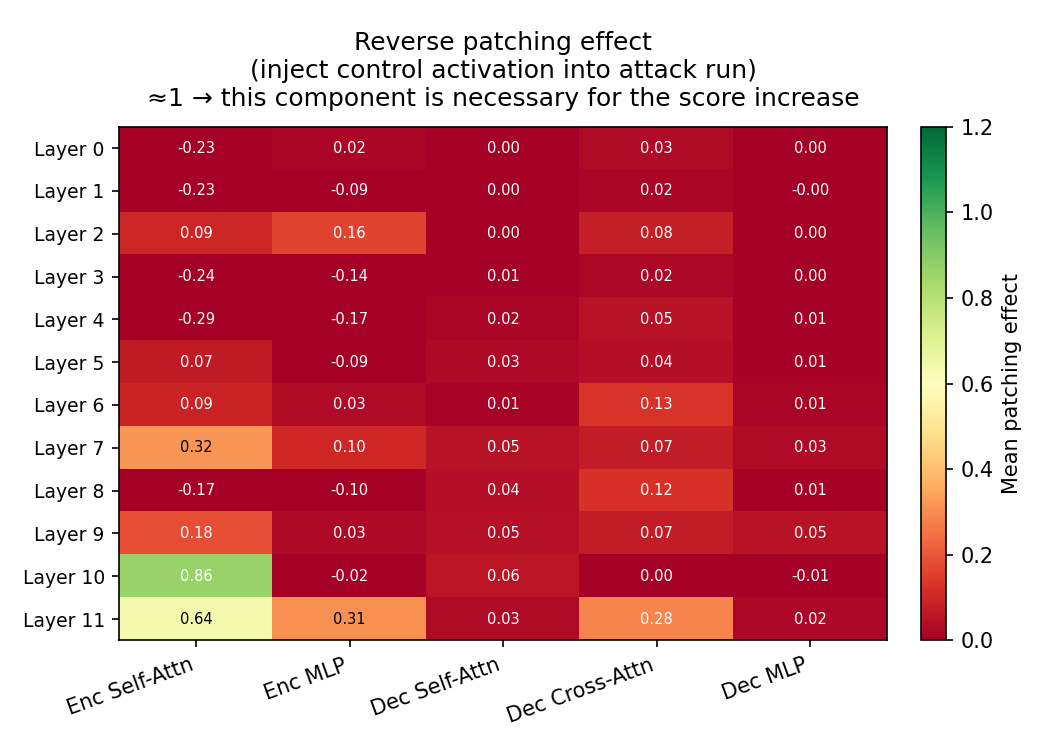
\includegraphics[width=0.17\textwidth]{outputs/attacks/information_start_2/plots/reverse_layer_component_heatmap.png} & 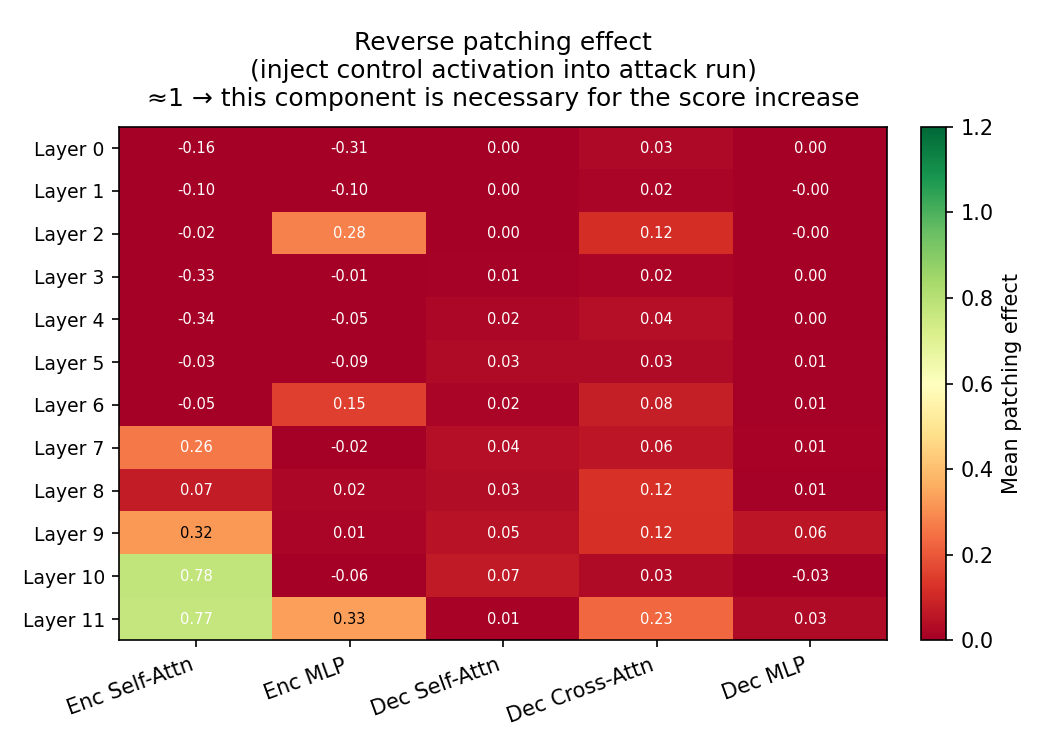
\includegraphics[width=0.17\textwidth]{outputs/attacks/information_start_3/plots/reverse_layer_component_heatmap.png} & 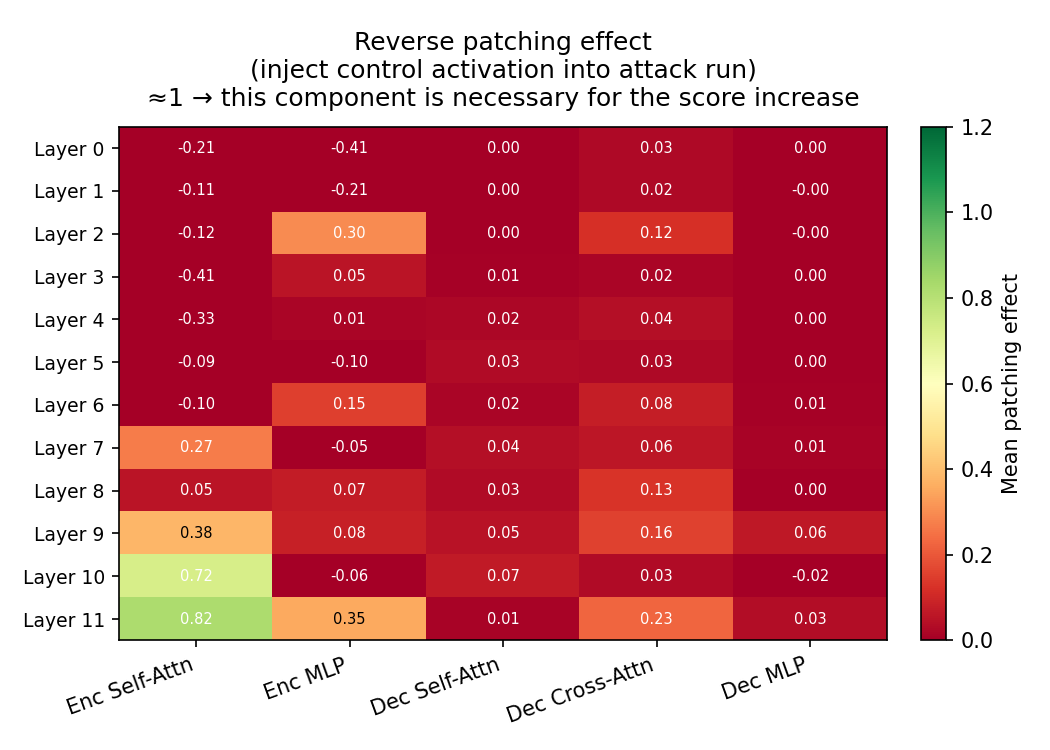
\includegraphics[width=0.17\textwidth]{outputs/attacks/information_start_4/plots/reverse_layer_component_heatmap.png} & 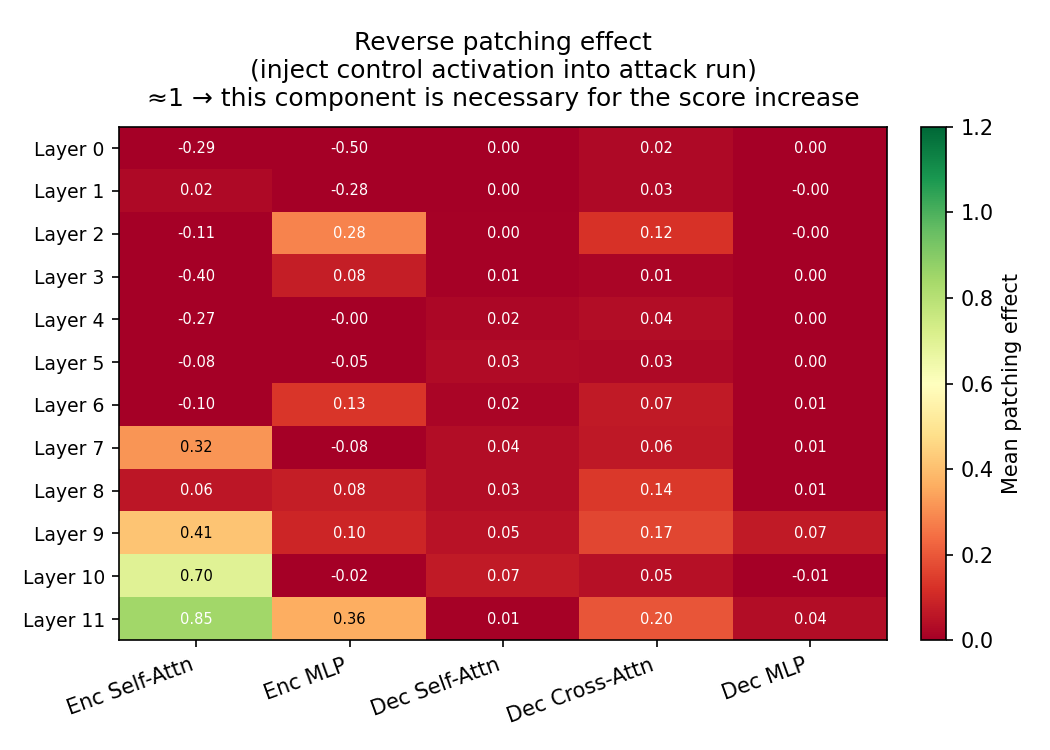
\includegraphics[width=0.17\textwidth]{outputs/attacks/information_start_5/plots/reverse_layer_component_heatmap.png} \\[4pt]
\rotatebox{90}{\textbf{combined}} & 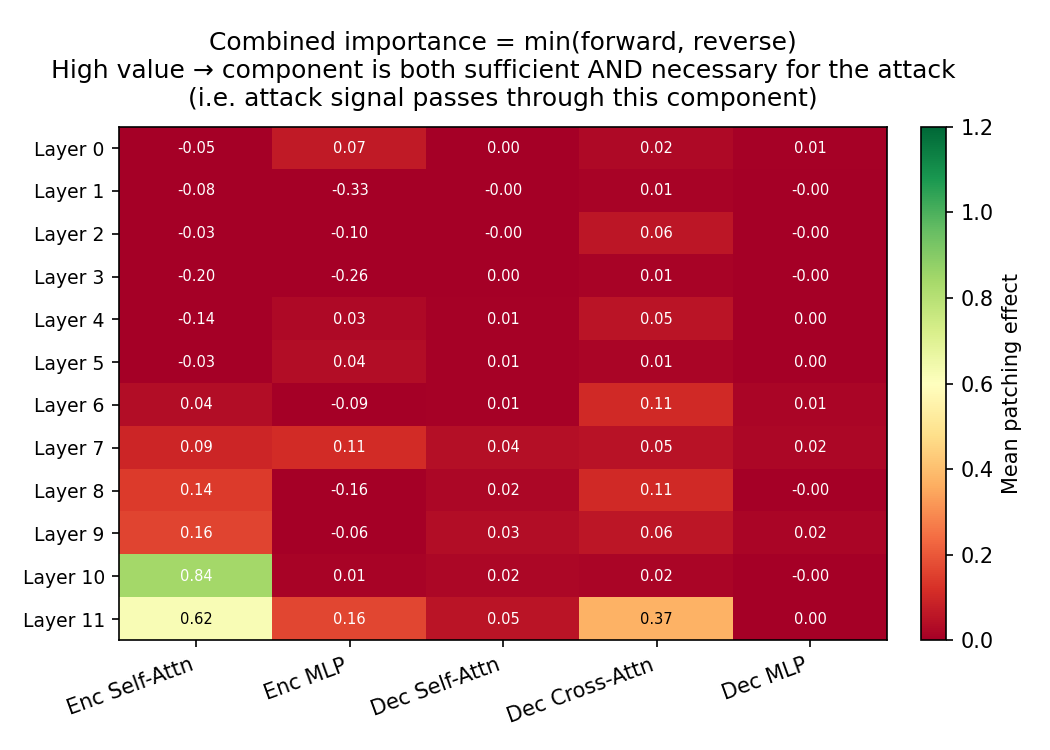
\includegraphics[width=0.17\textwidth]{outputs/attacks/information_start_1/plots/combined_layer_component_heatmap.png} & 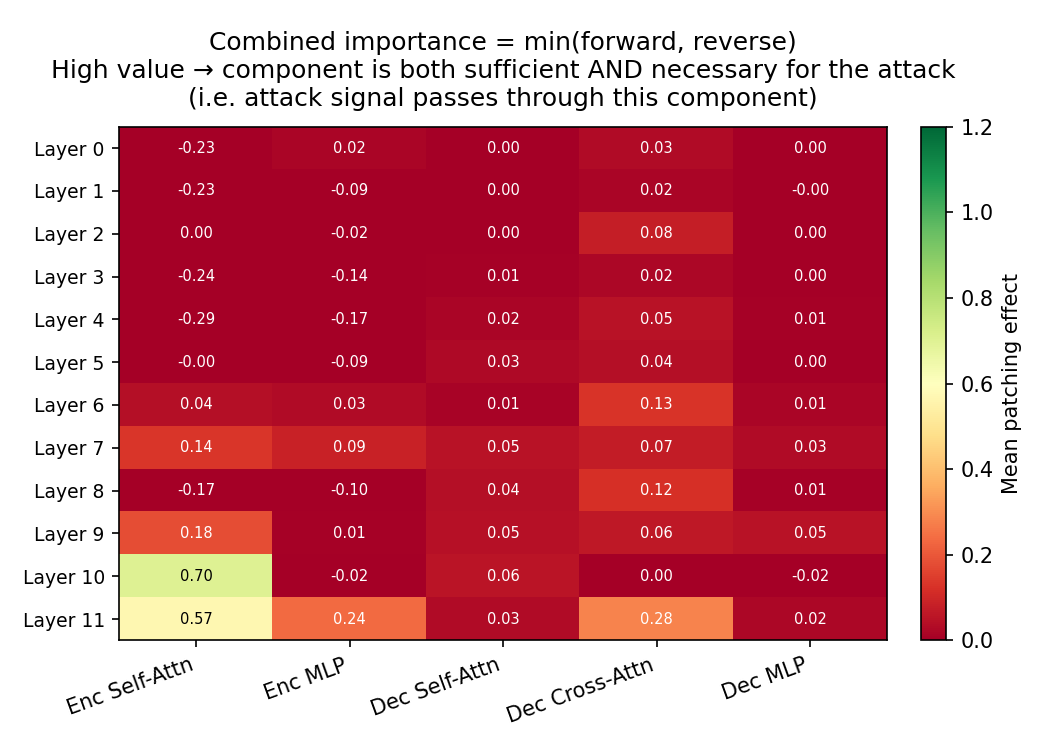
\includegraphics[width=0.17\textwidth]{outputs/attacks/information_start_2/plots/combined_layer_component_heatmap.png} & 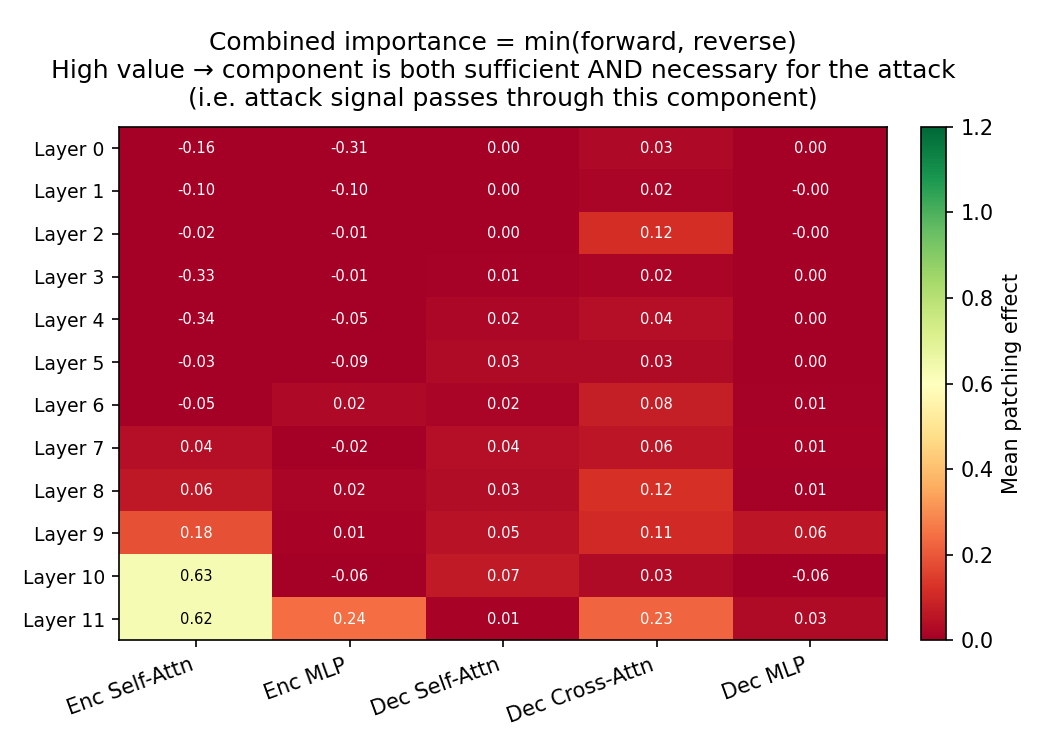
\includegraphics[width=0.17\textwidth]{outputs/attacks/information_start_3/plots/combined_layer_component_heatmap.png} & 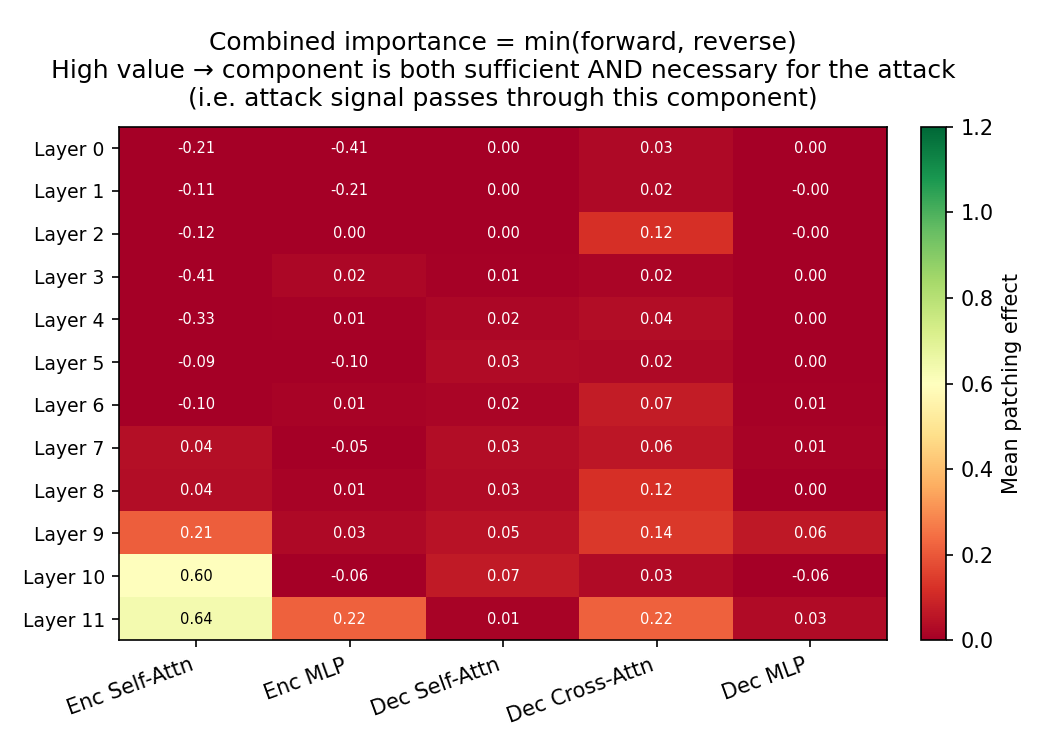
\includegraphics[width=0.17\textwidth]{outputs/attacks/information_start_4/plots/combined_layer_component_heatmap.png} & 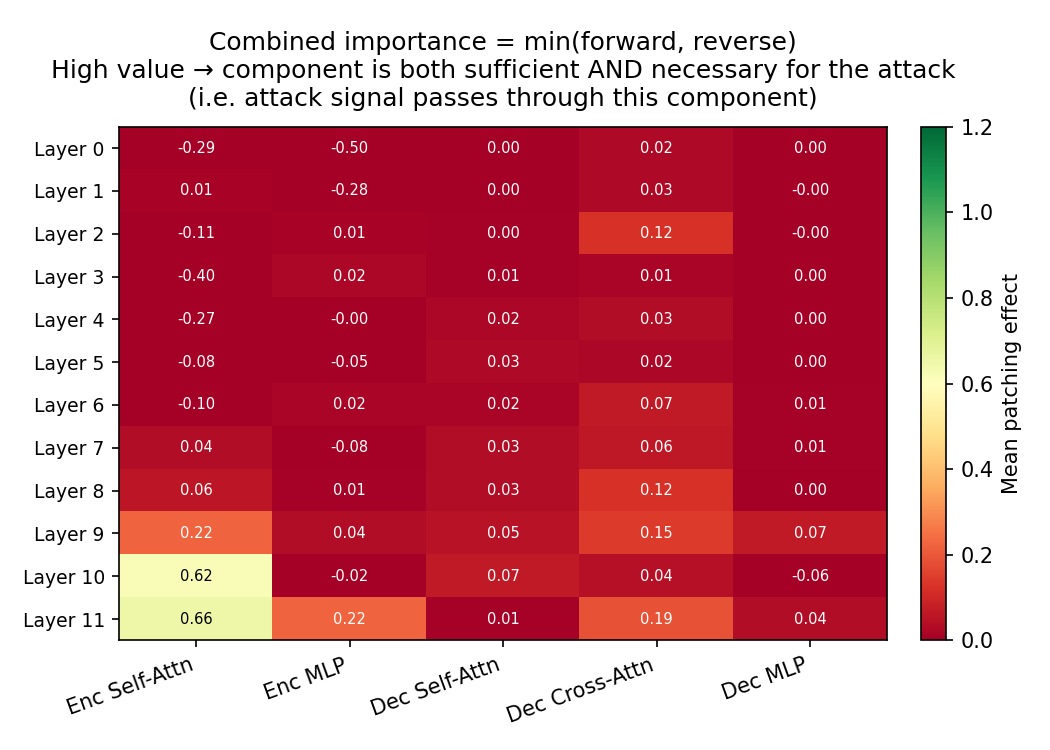
\includegraphics[width=0.17\textwidth]{outputs/attacks/information_start_5/plots/combined_layer_component_heatmap.png} \\[4pt]
\end{tabular}
\caption{Patching heatmaps for \texttt{information_start}: forward (top), reverse (middle), combined (bottom) across repetitions 1--5.}
\label{fig:hm:information_start}
\end{figure}

\begin{figure}[H]
\centering
\setlength{\tabcolsep}{2pt}
\renewcommand{\arraystretch}{0.5}
\begin{tabular}{r ccccc}
& \textbf{rep=1} & \textbf{rep=2} & \textbf{rep=3} & \textbf{rep=4} & \textbf{rep=5} \\[2pt]
\rotatebox{90}{\textbf{forward}} & 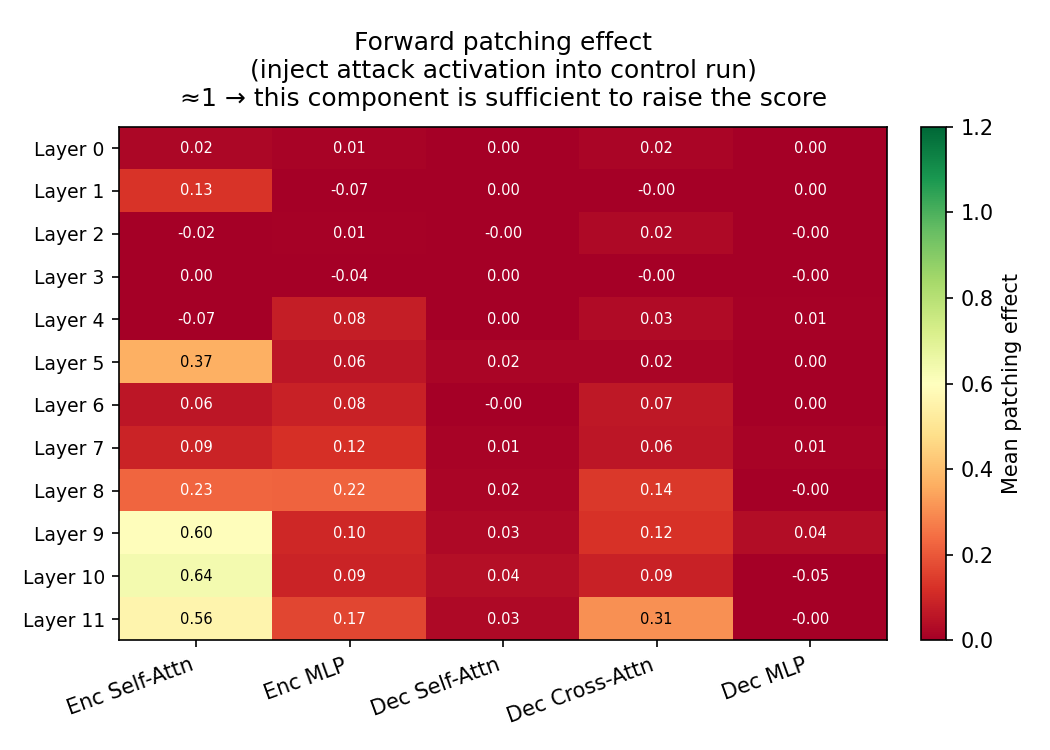
\includegraphics[width=0.17\textwidth]{outputs/attacks/relevance_end_1/plots/forward_layer_component_heatmap.png} & 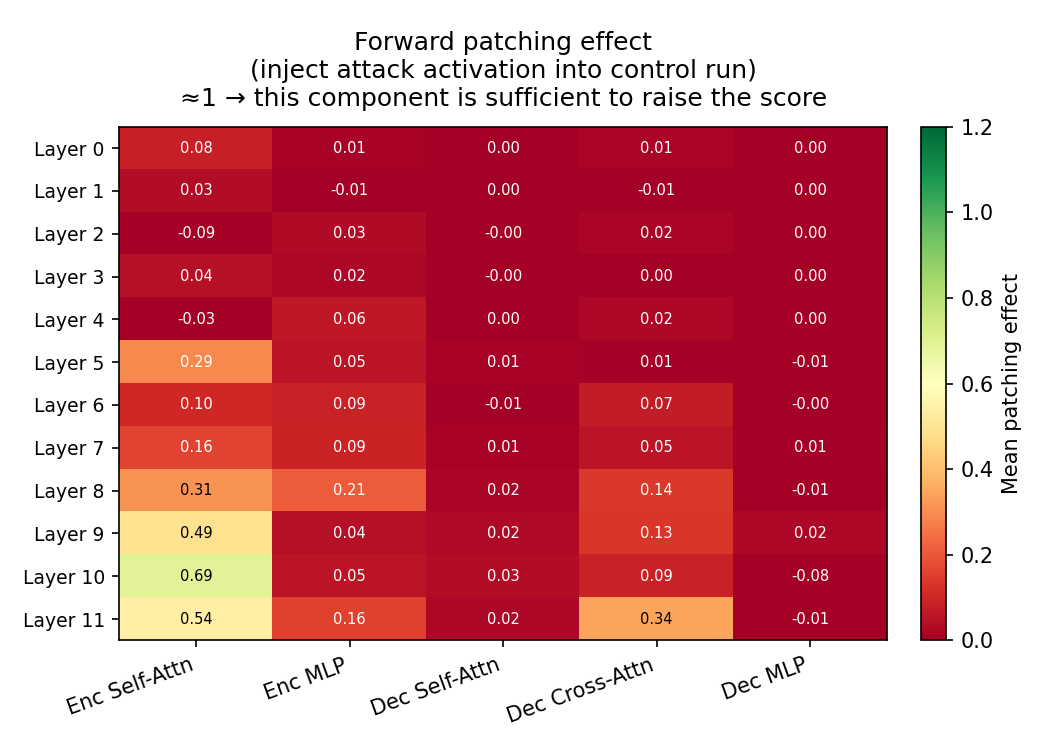
\includegraphics[width=0.17\textwidth]{outputs/attacks/relevance_end_2/plots/forward_layer_component_heatmap.png} & 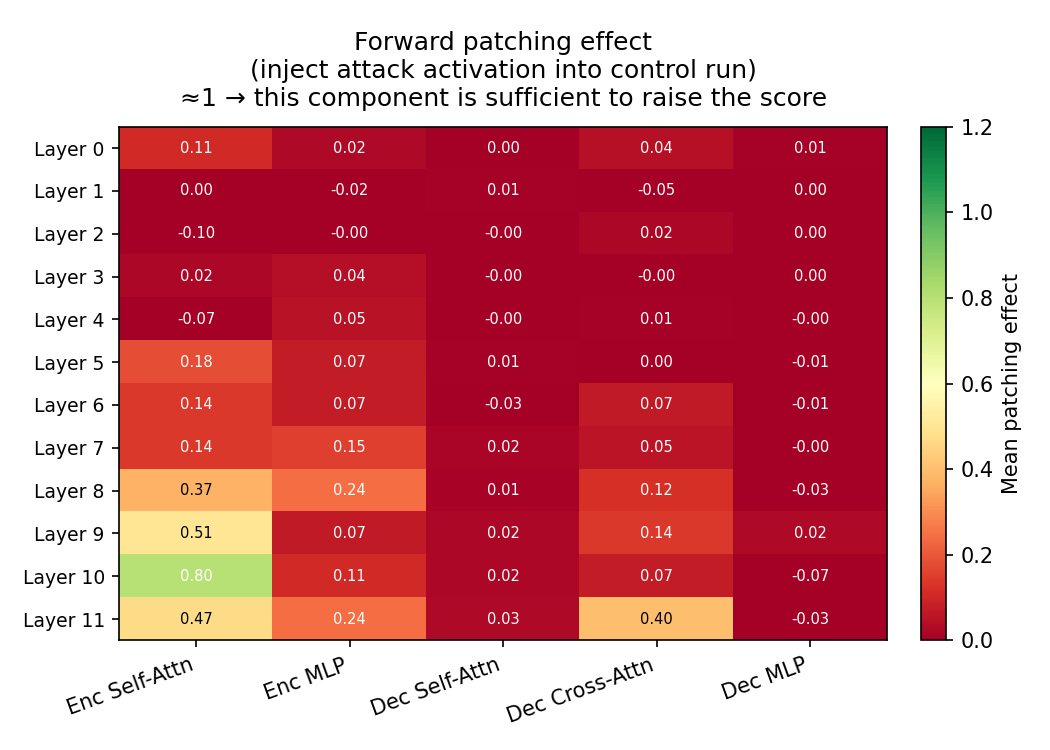
\includegraphics[width=0.17\textwidth]{outputs/attacks/relevance_end_3/plots/forward_layer_component_heatmap.png} & 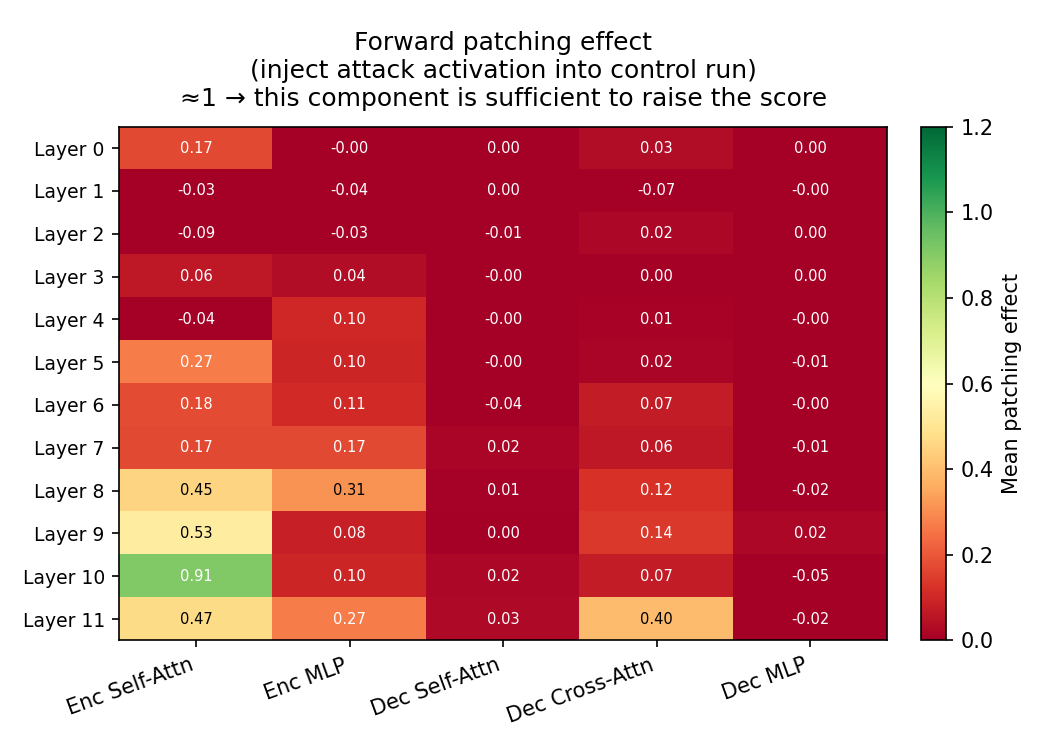
\includegraphics[width=0.17\textwidth]{outputs/attacks/relevance_end_4/plots/forward_layer_component_heatmap.png} & 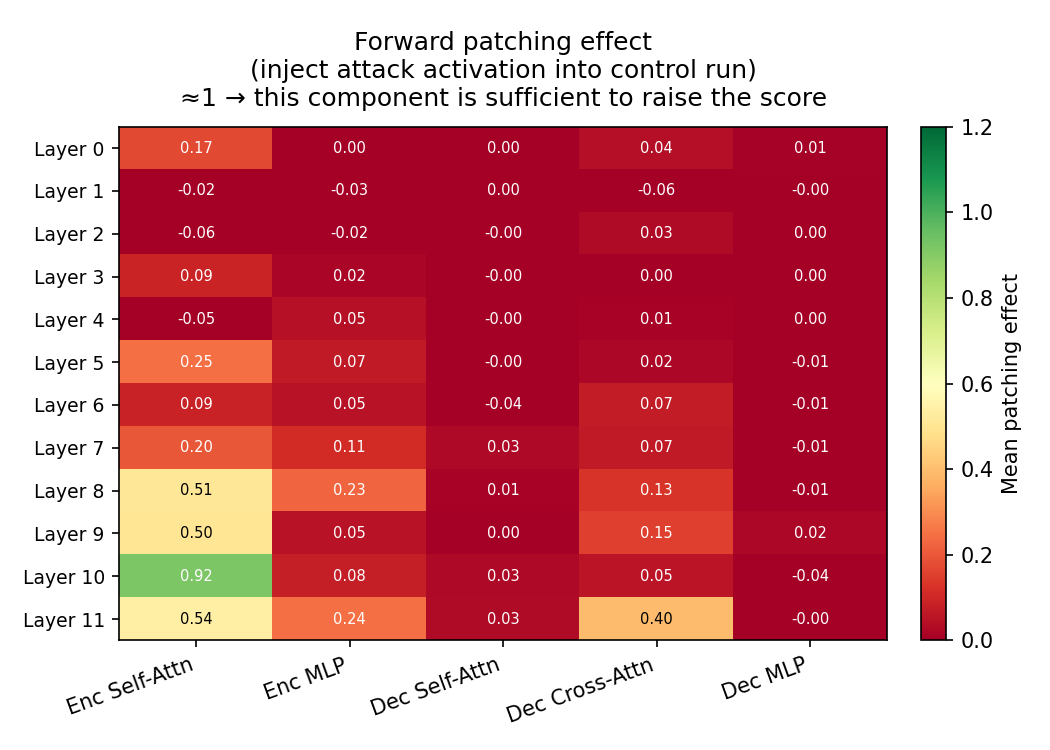
\includegraphics[width=0.17\textwidth]{outputs/attacks/relevance_end_5/plots/forward_layer_component_heatmap.png} \\[4pt]
\rotatebox{90}{\textbf{reverse}} & 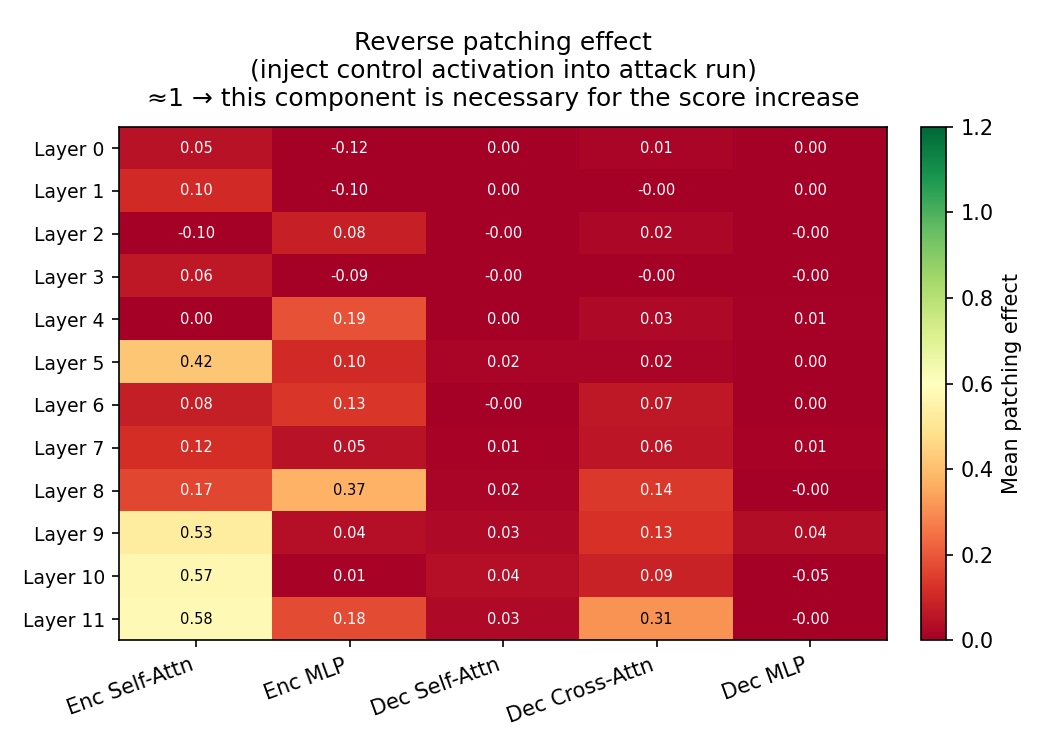
\includegraphics[width=0.17\textwidth]{outputs/attacks/relevance_end_1/plots/reverse_layer_component_heatmap.png} & 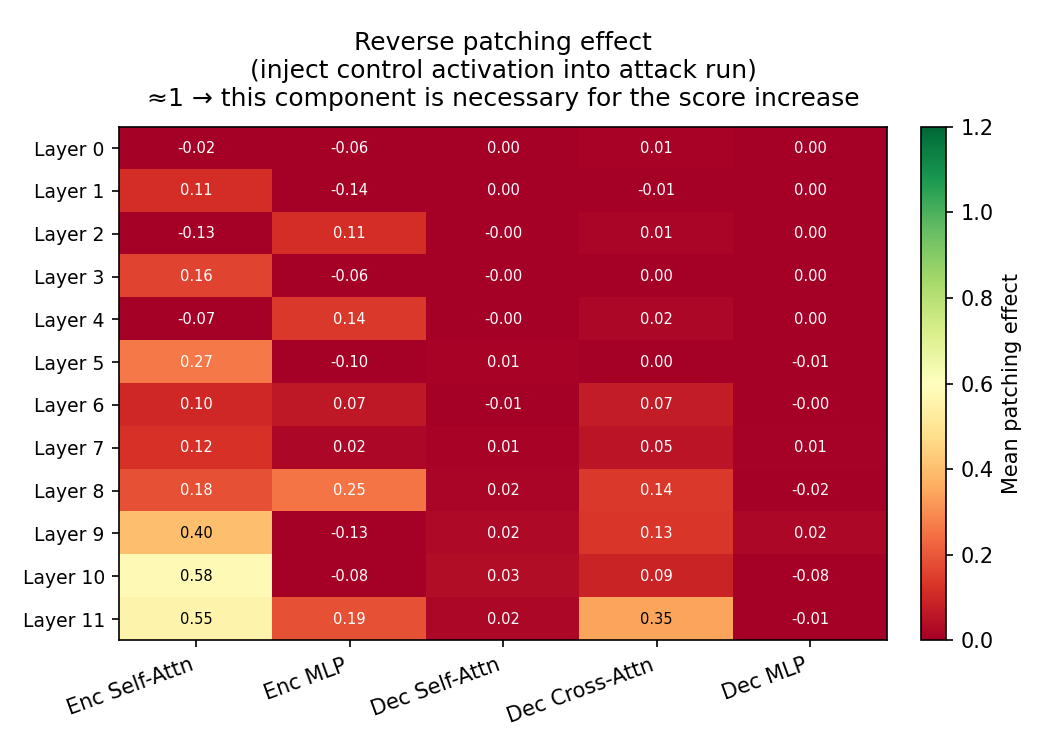
\includegraphics[width=0.17\textwidth]{outputs/attacks/relevance_end_2/plots/reverse_layer_component_heatmap.png} & 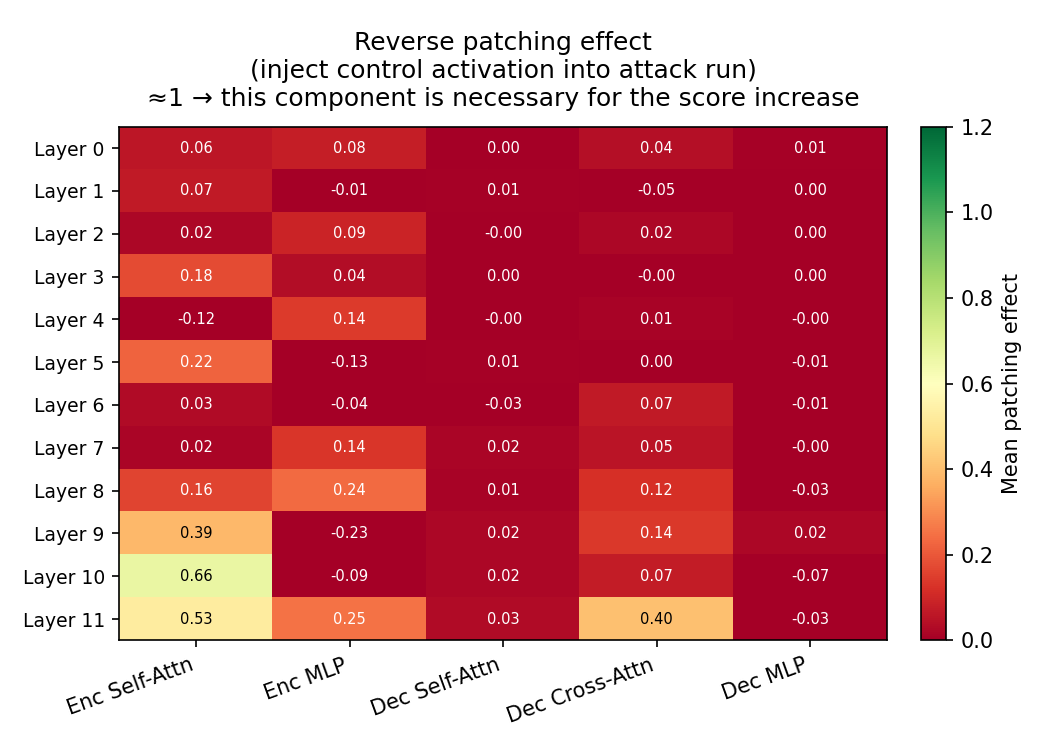
\includegraphics[width=0.17\textwidth]{outputs/attacks/relevance_end_3/plots/reverse_layer_component_heatmap.png} & 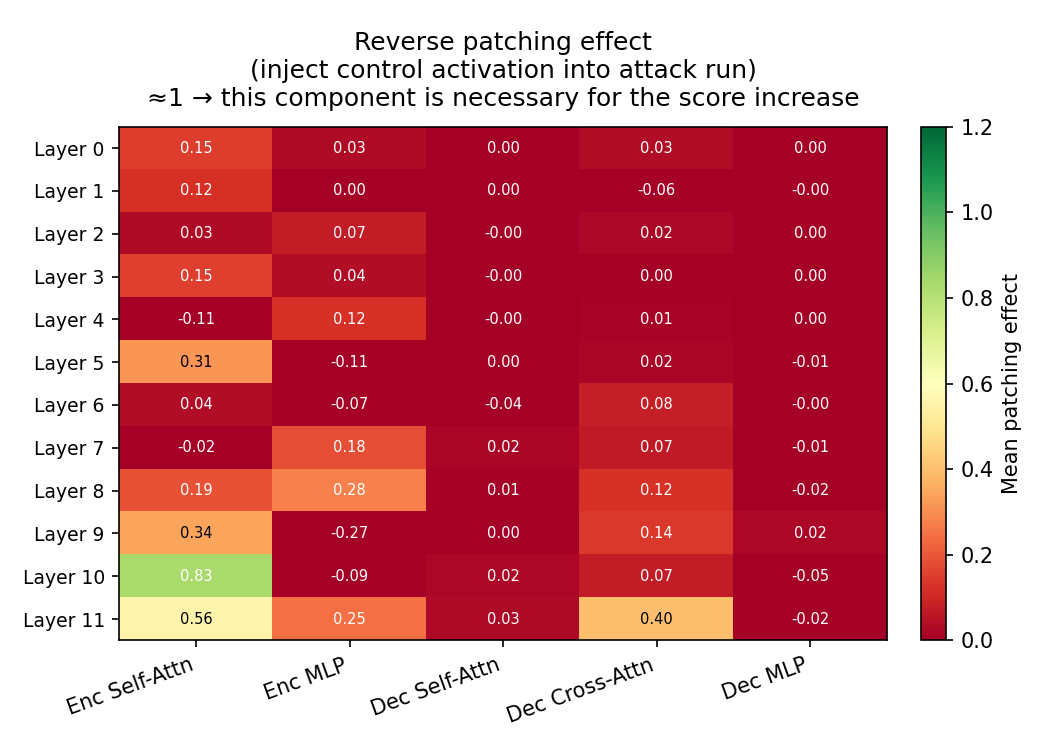
\includegraphics[width=0.17\textwidth]{outputs/attacks/relevance_end_4/plots/reverse_layer_component_heatmap.png} & 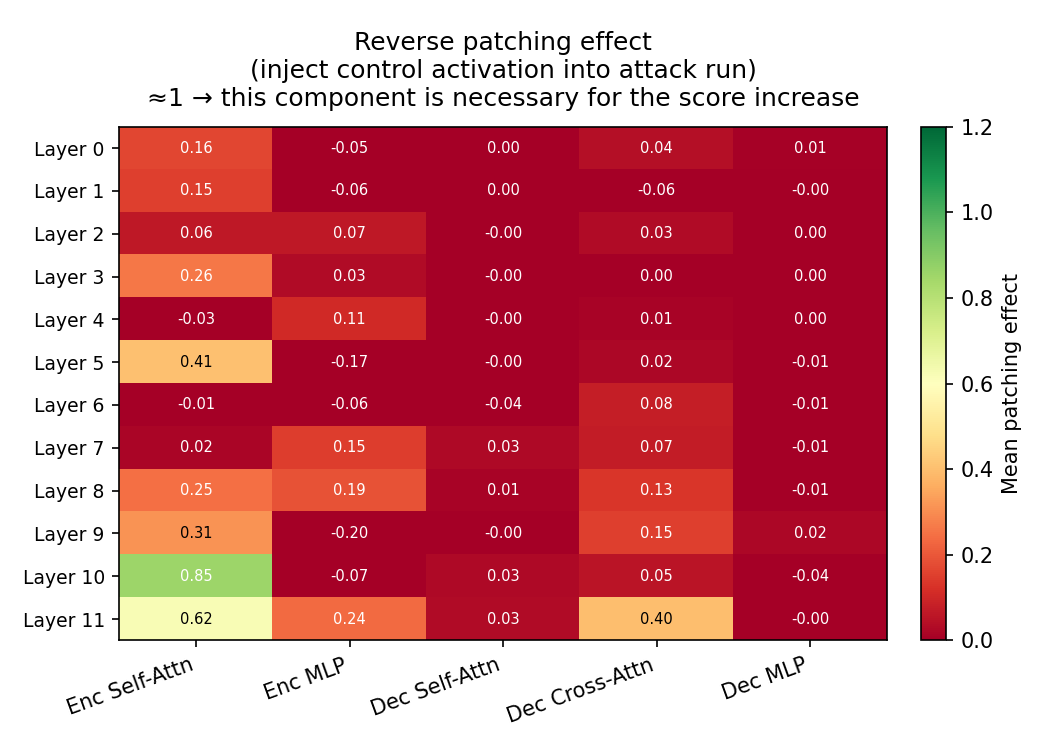
\includegraphics[width=0.17\textwidth]{outputs/attacks/relevance_end_5/plots/reverse_layer_component_heatmap.png} \\[4pt]
\rotatebox{90}{\textbf{combined}} & 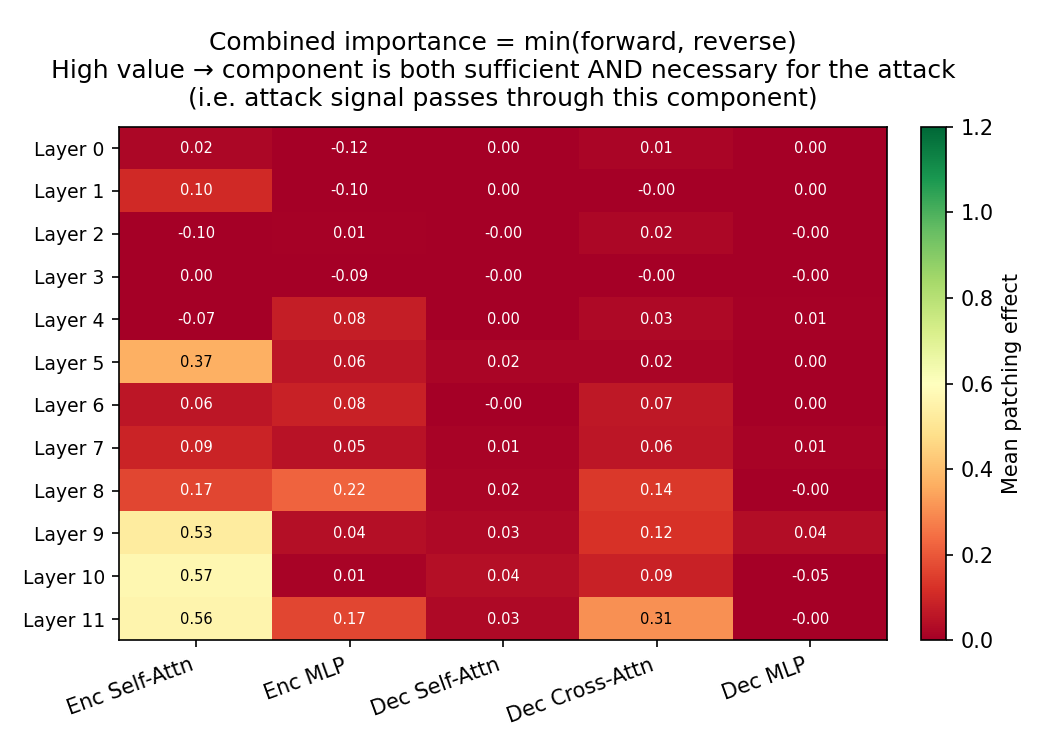
\includegraphics[width=0.17\textwidth]{outputs/attacks/relevance_end_1/plots/combined_layer_component_heatmap.png} & 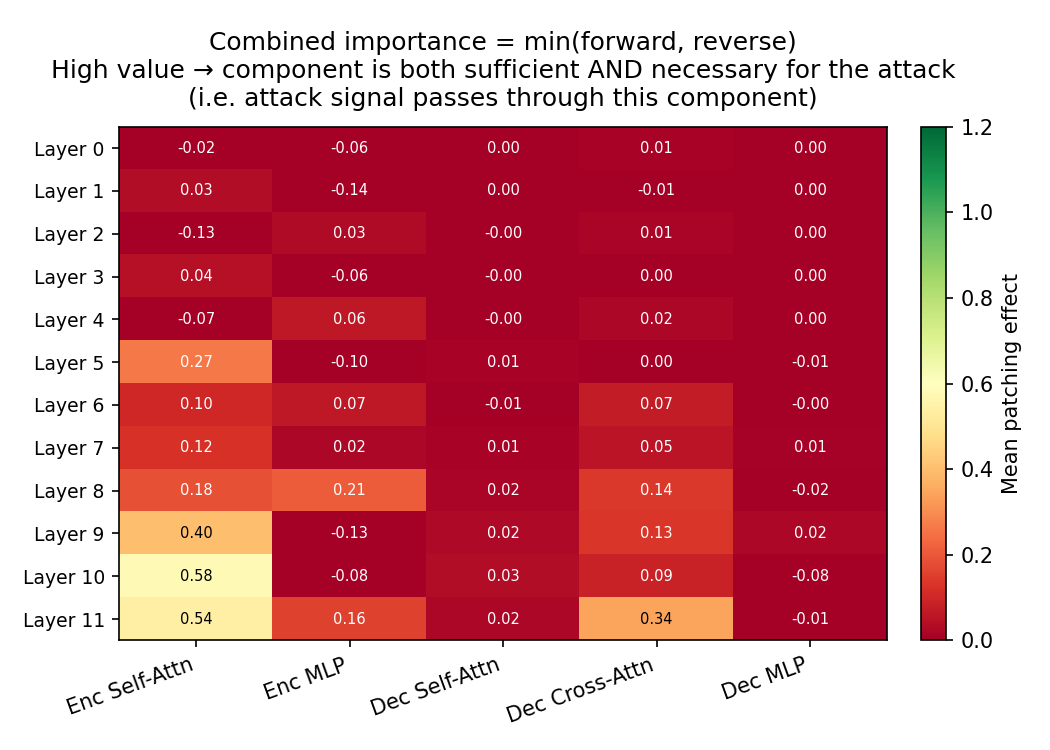
\includegraphics[width=0.17\textwidth]{outputs/attacks/relevance_end_2/plots/combined_layer_component_heatmap.png} & 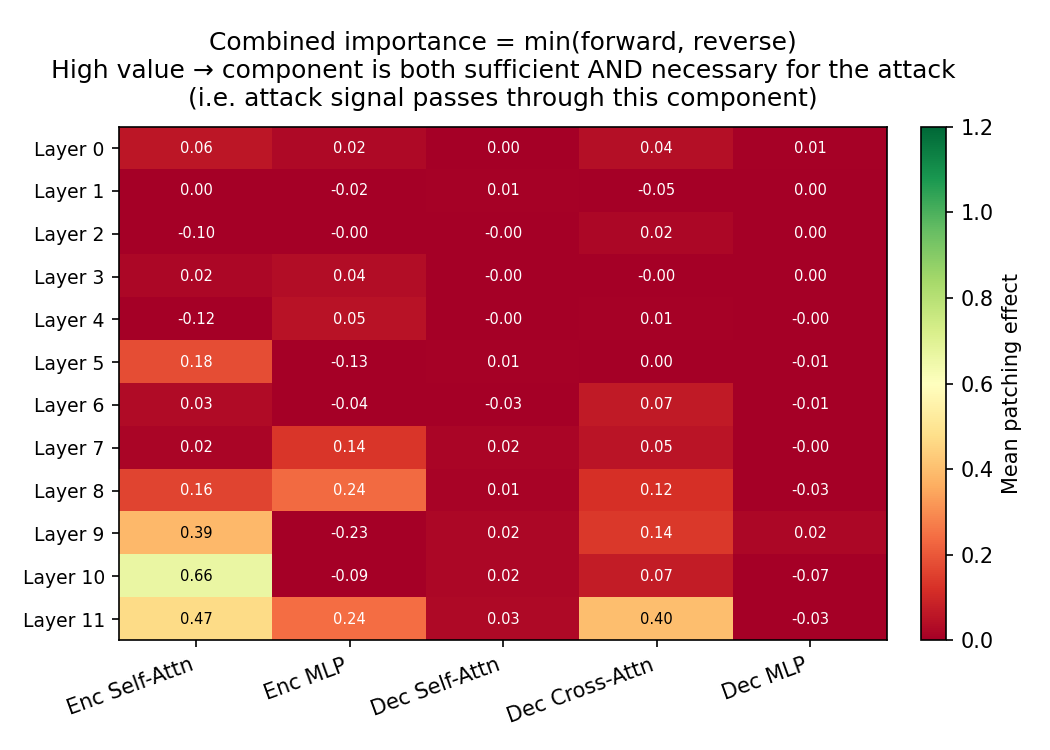
\includegraphics[width=0.17\textwidth]{outputs/attacks/relevance_end_3/plots/combined_layer_component_heatmap.png} & 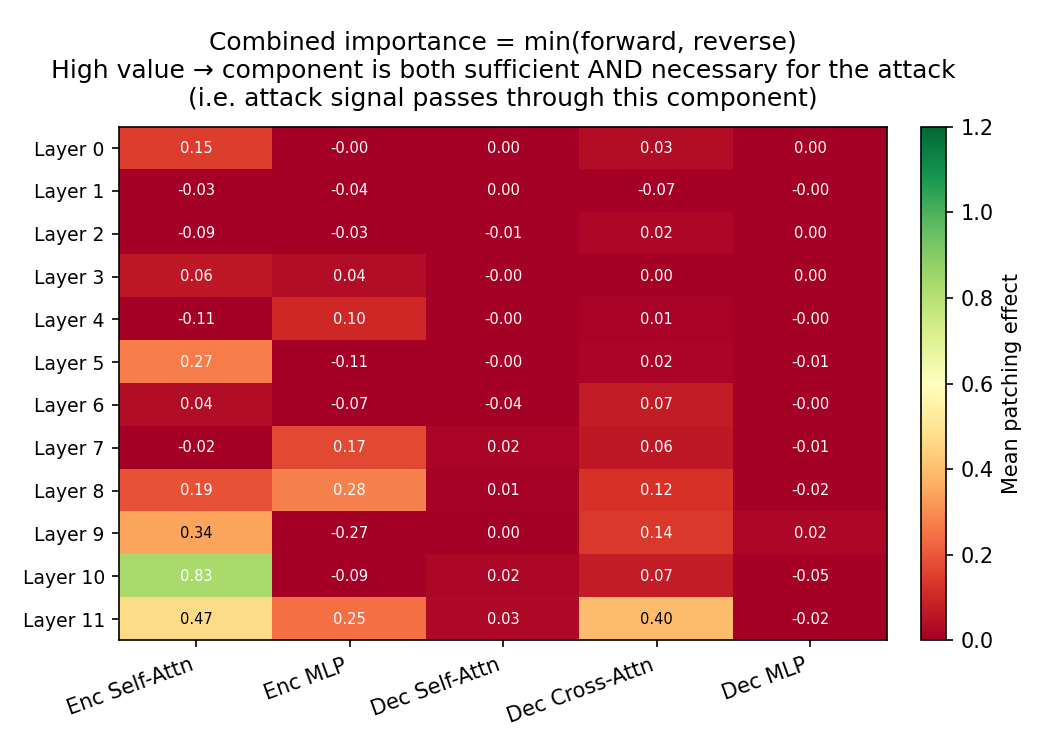
\includegraphics[width=0.17\textwidth]{outputs/attacks/relevance_end_4/plots/combined_layer_component_heatmap.png} & 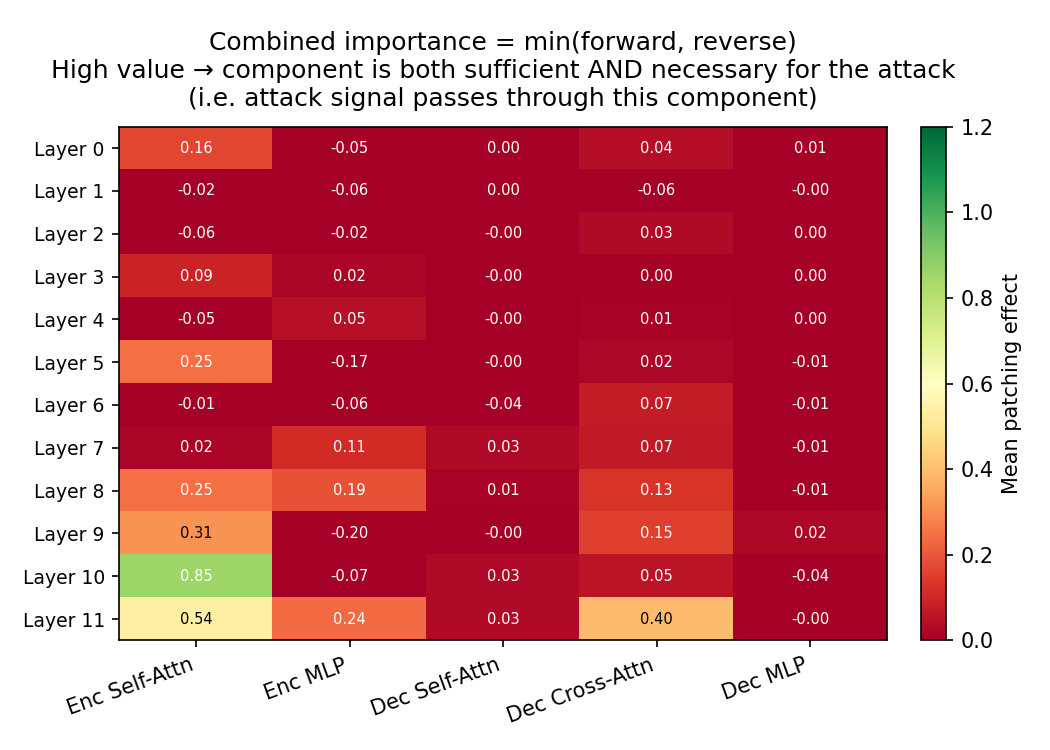
\includegraphics[width=0.17\textwidth]{outputs/attacks/relevance_end_5/plots/combined_layer_component_heatmap.png} \\[4pt]
\end{tabular}
\caption{Patching heatmaps for \texttt{relevance_end}: forward (top), reverse (middle), combined (bottom) across repetitions 1--5.}
\label{fig:hm:relevance_end}
\end{figure}

\begin{figure}[H]
\centering
\setlength{\tabcolsep}{2pt}
\renewcommand{\arraystretch}{0.5}
\begin{tabular}{r ccccc}
& \textbf{rep=1} & \textbf{rep=2} & \textbf{rep=3} & \textbf{rep=4} & \textbf{rep=5} \\[2pt]
\rotatebox{90}{\textbf{forward}} & 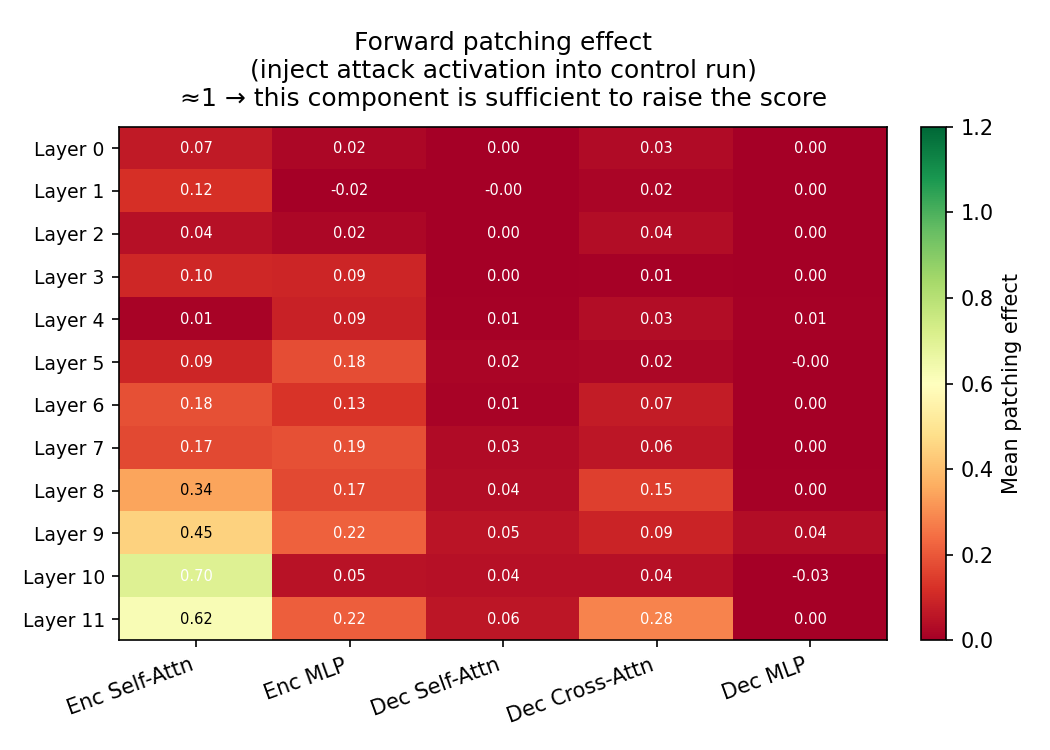
\includegraphics[width=0.17\textwidth]{outputs/attacks/relevance_random_1/plots/forward_layer_component_heatmap.png} & 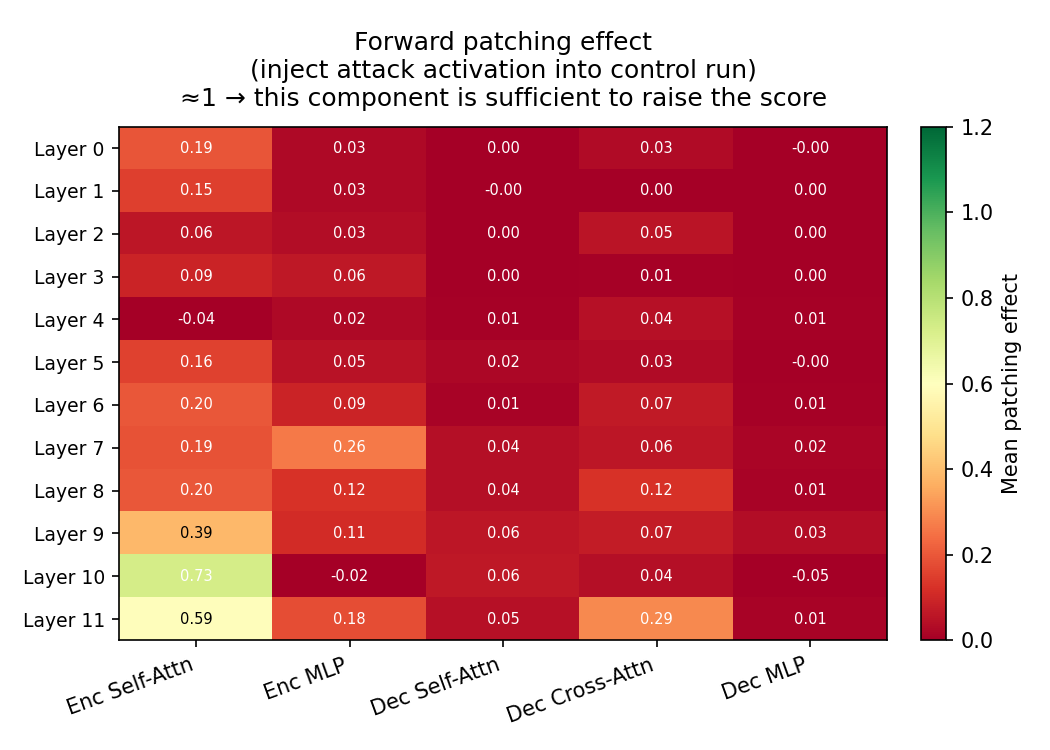
\includegraphics[width=0.17\textwidth]{outputs/attacks/relevance_random_2/plots/forward_layer_component_heatmap.png} & 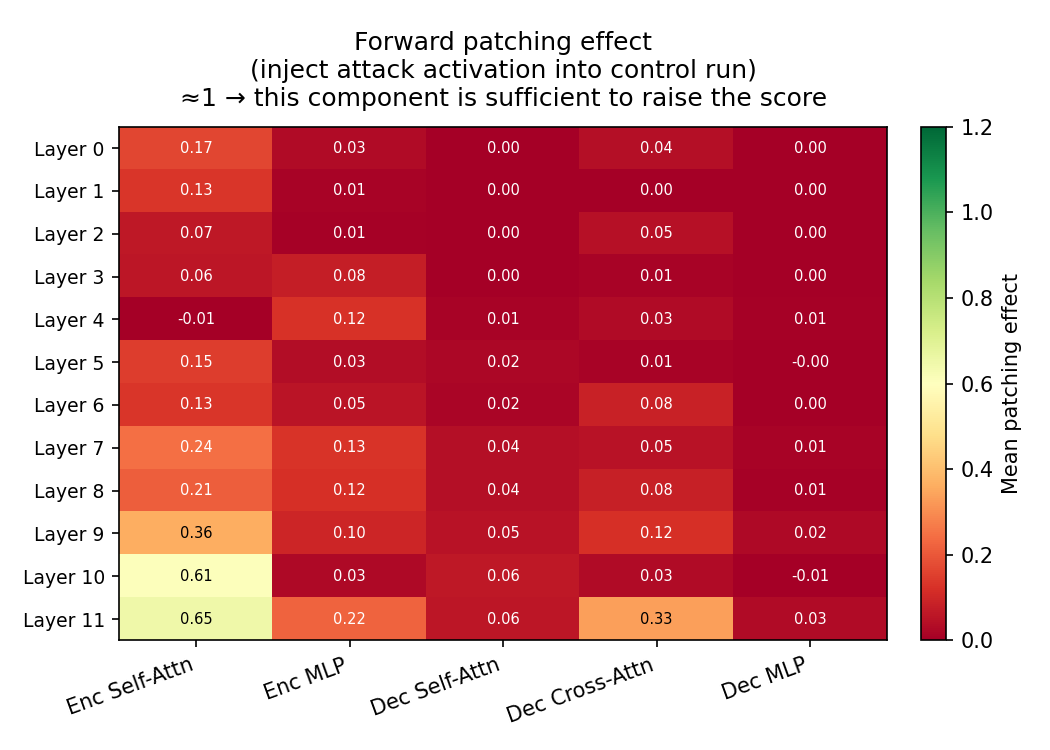
\includegraphics[width=0.17\textwidth]{outputs/attacks/relevance_random_3/plots/forward_layer_component_heatmap.png} & 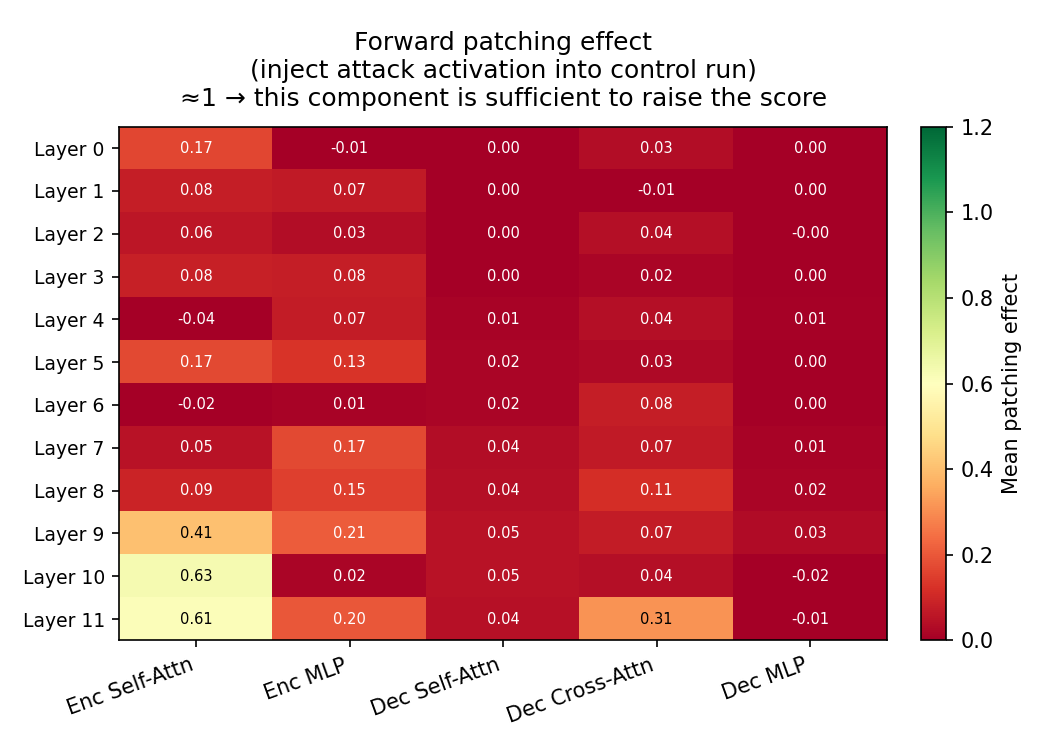
\includegraphics[width=0.17\textwidth]{outputs/attacks/relevance_random_4/plots/forward_layer_component_heatmap.png} & 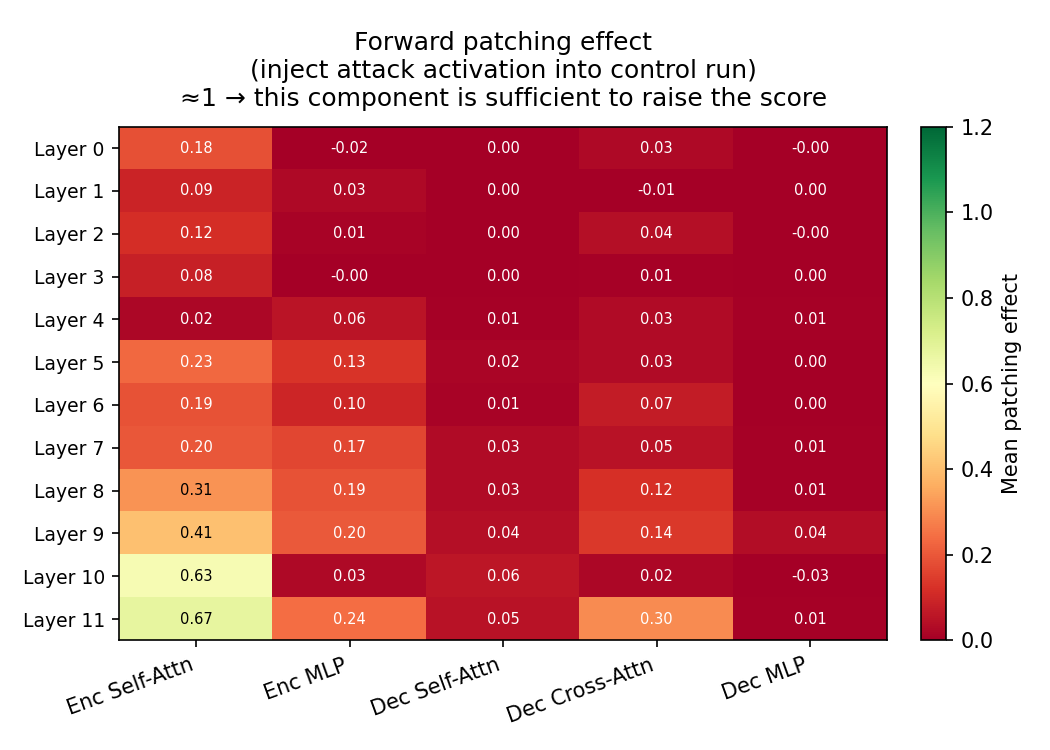
\includegraphics[width=0.17\textwidth]{outputs/attacks/relevance_random_5/plots/forward_layer_component_heatmap.png} \\[4pt]
\rotatebox{90}{\textbf{reverse}} & \includegraphics[width=0.17\textwidth]{outputs/attacks/relevance_random_1/plots/reverse_layer_component_heatmap.png} & \includegraphics[width=0.17\textwidth]{outputs/attacks/relevance_random_2/plots/reverse_layer_component_heatmap.png} & \includegraphics[width=0.17\textwidth]{outputs/attacks/relevance_random_3/plots/reverse_layer_component_heatmap.png} & \includegraphics[width=0.17\textwidth]{outputs/attacks/relevance_random_4/plots/reverse_layer_component_heatmap.png} & \includegraphics[width=0.17\textwidth]{outputs/attacks/relevance_random_5/plots/reverse_layer_component_heatmap.png} \\[4pt]
\rotatebox{90}{\textbf{combined}} & \includegraphics[width=0.17\textwidth]{outputs/attacks/relevance_random_1/plots/combined_layer_component_heatmap.png} & \includegraphics[width=0.17\textwidth]{outputs/attacks/relevance_random_2/plots/combined_layer_component_heatmap.png} & \includegraphics[width=0.17\textwidth]{outputs/attacks/relevance_random_3/plots/combined_layer_component_heatmap.png} & \includegraphics[width=0.17\textwidth]{outputs/attacks/relevance_random_4/plots/combined_layer_component_heatmap.png} & \includegraphics[width=0.17\textwidth]{outputs/attacks/relevance_random_5/plots/combined_layer_component_heatmap.png} \\[4pt]
\end{tabular}
\caption{Patching heatmaps for \texttt{relevance_random}: forward (top), reverse (middle), combined (bottom) across repetitions 1--5.}
\label{fig:hm:relevance_random}
\end{figure}

\begin{figure}[H]
\centering
\setlength{\tabcolsep}{2pt}
\renewcommand{\arraystretch}{0.5}
\begin{tabular}{r ccccc}
& \textbf{rep=1} & \textbf{rep=2} & \textbf{rep=3} & \textbf{rep=4} & \textbf{rep=5} \\[2pt]
\rotatebox{90}{\textbf{forward}} & \includegraphics[width=0.17\textwidth]{outputs/attacks/relevance_start_1/plots/forward_layer_component_heatmap.png} & \includegraphics[width=0.17\textwidth]{outputs/attacks/relevance_start_2/plots/forward_layer_component_heatmap.png} & \includegraphics[width=0.17\textwidth]{outputs/attacks/relevance_start_3/plots/forward_layer_component_heatmap.png} & \includegraphics[width=0.17\textwidth]{outputs/attacks/relevance_start_4/plots/forward_layer_component_heatmap.png} & \includegraphics[width=0.17\textwidth]{outputs/attacks/relevance_start_5/plots/forward_layer_component_heatmap.png} \\[4pt]
\rotatebox{90}{\textbf{reverse}} & \includegraphics[width=0.17\textwidth]{outputs/attacks/relevance_start_1/plots/reverse_layer_component_heatmap.png} & \includegraphics[width=0.17\textwidth]{outputs/attacks/relevance_start_2/plots/reverse_layer_component_heatmap.png} & \includegraphics[width=0.17\textwidth]{outputs/attacks/relevance_start_3/plots/reverse_layer_component_heatmap.png} & \includegraphics[width=0.17\textwidth]{outputs/attacks/relevance_start_4/plots/reverse_layer_component_heatmap.png} & \includegraphics[width=0.17\textwidth]{outputs/attacks/relevance_start_5/plots/reverse_layer_component_heatmap.png} \\[4pt]
\rotatebox{90}{\textbf{combined}} & \includegraphics[width=0.17\textwidth]{outputs/attacks/relevance_start_1/plots/combined_layer_component_heatmap.png} & \includegraphics[width=0.17\textwidth]{outputs/attacks/relevance_start_2/plots/combined_layer_component_heatmap.png} & \includegraphics[width=0.17\textwidth]{outputs/attacks/relevance_start_3/plots/combined_layer_component_heatmap.png} & \includegraphics[width=0.17\textwidth]{outputs/attacks/relevance_start_4/plots/combined_layer_component_heatmap.png} & \includegraphics[width=0.17\textwidth]{outputs/attacks/relevance_start_5/plots/combined_layer_component_heatmap.png} \\[4pt]
\end{tabular}
\caption{Patching heatmaps for \texttt{relevance_start}: forward (top), reverse (middle), combined (bottom) across repetitions 1--5.}
\label{fig:hm:relevance_start}
\end{figure}

\begin{figure}[H]
\centering
\setlength{\tabcolsep}{2pt}
\renewcommand{\arraystretch}{0.5}
\begin{tabular}{r ccccc}
& \textbf{rep=1} & \textbf{rep=2} & \textbf{rep=3} & \textbf{rep=4} & \textbf{rep=5} \\[2pt]
\rotatebox{90}{\textbf{forward}} & \includegraphics[width=0.17\textwidth]{outputs/attacks/relevant_end_1/plots/forward_layer_component_heatmap.png} & \includegraphics[width=0.17\textwidth]{outputs/attacks/relevant_end_2/plots/forward_layer_component_heatmap.png} & \includegraphics[width=0.17\textwidth]{outputs/attacks/relevant_end_3/plots/forward_layer_component_heatmap.png} & \includegraphics[width=0.17\textwidth]{outputs/attacks/relevant_end_4/plots/forward_layer_component_heatmap.png} & \includegraphics[width=0.17\textwidth]{outputs/attacks/relevant_end_5/plots/forward_layer_component_heatmap.png} \\[4pt]
\rotatebox{90}{\textbf{reverse}} & \includegraphics[width=0.17\textwidth]{outputs/attacks/relevant_end_1/plots/reverse_layer_component_heatmap.png} & \includegraphics[width=0.17\textwidth]{outputs/attacks/relevant_end_2/plots/reverse_layer_component_heatmap.png} & \includegraphics[width=0.17\textwidth]{outputs/attacks/relevant_end_3/plots/reverse_layer_component_heatmap.png} & \includegraphics[width=0.17\textwidth]{outputs/attacks/relevant_end_4/plots/reverse_layer_component_heatmap.png} & \includegraphics[width=0.17\textwidth]{outputs/attacks/relevant_end_5/plots/reverse_layer_component_heatmap.png} \\[4pt]
\rotatebox{90}{\textbf{combined}} & \includegraphics[width=0.17\textwidth]{outputs/attacks/relevant_end_1/plots/combined_layer_component_heatmap.png} & \includegraphics[width=0.17\textwidth]{outputs/attacks/relevant_end_2/plots/combined_layer_component_heatmap.png} & \includegraphics[width=0.17\textwidth]{outputs/attacks/relevant_end_3/plots/combined_layer_component_heatmap.png} & \includegraphics[width=0.17\textwidth]{outputs/attacks/relevant_end_4/plots/combined_layer_component_heatmap.png} & \includegraphics[width=0.17\textwidth]{outputs/attacks/relevant_end_5/plots/combined_layer_component_heatmap.png} \\[4pt]
\end{tabular}
\caption{Patching heatmaps for \texttt{relevant_end}: forward (top), reverse (middle), combined (bottom) across repetitions 1--5.}
\label{fig:hm:relevant_end}
\end{figure}

\begin{figure}[H]
\centering
\setlength{\tabcolsep}{2pt}
\renewcommand{\arraystretch}{0.5}
\begin{tabular}{r ccccc}
& \textbf{rep=1} & \textbf{rep=2} & \textbf{rep=3} & \textbf{rep=4} & \textbf{rep=5} \\[2pt]
\rotatebox{90}{\textbf{forward}} & \includegraphics[width=0.17\textwidth]{outputs/attacks/relevant_random_1/plots/forward_layer_component_heatmap.png} & \includegraphics[width=0.17\textwidth]{outputs/attacks/relevant_random_2/plots/forward_layer_component_heatmap.png} & \includegraphics[width=0.17\textwidth]{outputs/attacks/relevant_random_3/plots/forward_layer_component_heatmap.png} & \includegraphics[width=0.17\textwidth]{outputs/attacks/relevant_random_4/plots/forward_layer_component_heatmap.png} & \includegraphics[width=0.17\textwidth]{outputs/attacks/relevant_random_5/plots/forward_layer_component_heatmap.png} \\[4pt]
\rotatebox{90}{\textbf{reverse}} & \includegraphics[width=0.17\textwidth]{outputs/attacks/relevant_random_1/plots/reverse_layer_component_heatmap.png} & \includegraphics[width=0.17\textwidth]{outputs/attacks/relevant_random_2/plots/reverse_layer_component_heatmap.png} & \includegraphics[width=0.17\textwidth]{outputs/attacks/relevant_random_3/plots/reverse_layer_component_heatmap.png} & \includegraphics[width=0.17\textwidth]{outputs/attacks/relevant_random_4/plots/reverse_layer_component_heatmap.png} & \includegraphics[width=0.17\textwidth]{outputs/attacks/relevant_random_5/plots/reverse_layer_component_heatmap.png} \\[4pt]
\rotatebox{90}{\textbf{combined}} & \includegraphics[width=0.17\textwidth]{outputs/attacks/relevant_random_1/plots/combined_layer_component_heatmap.png} & \includegraphics[width=0.17\textwidth]{outputs/attacks/relevant_random_2/plots/combined_layer_component_heatmap.png} & \includegraphics[width=0.17\textwidth]{outputs/attacks/relevant_random_3/plots/combined_layer_component_heatmap.png} & \includegraphics[width=0.17\textwidth]{outputs/attacks/relevant_random_4/plots/combined_layer_component_heatmap.png} & \includegraphics[width=0.17\textwidth]{outputs/attacks/relevant_random_5/plots/combined_layer_component_heatmap.png} \\[4pt]
\end{tabular}
\caption{Patching heatmaps for \texttt{relevant_random}: forward (top), reverse (middle), combined (bottom) across repetitions 1--5.}
\label{fig:hm:relevant_random}
\end{figure}

\begin{figure}[H]
\centering
\setlength{\tabcolsep}{2pt}
\renewcommand{\arraystretch}{0.5}
\begin{tabular}{r ccccc}
& \textbf{rep=1} & \textbf{rep=2} & \textbf{rep=3} & \textbf{rep=4} & \textbf{rep=5} \\[2pt]
\rotatebox{90}{\textbf{forward}} & \includegraphics[width=0.17\textwidth]{outputs/attacks/relevant_start_1/plots/forward_layer_component_heatmap.png} & \includegraphics[width=0.17\textwidth]{outputs/attacks/relevant_start_2/plots/forward_layer_component_heatmap.png} & \includegraphics[width=0.17\textwidth]{outputs/attacks/relevant_start_3/plots/forward_layer_component_heatmap.png} & \includegraphics[width=0.17\textwidth]{outputs/attacks/relevant_start_4/plots/forward_layer_component_heatmap.png} & \includegraphics[width=0.17\textwidth]{outputs/attacks/relevant_start_5/plots/forward_layer_component_heatmap.png} \\[4pt]
\rotatebox{90}{\textbf{reverse}} & \includegraphics[width=0.17\textwidth]{outputs/attacks/relevant_start_1/plots/reverse_layer_component_heatmap.png} & \includegraphics[width=0.17\textwidth]{outputs/attacks/relevant_start_2/plots/reverse_layer_component_heatmap.png} & \includegraphics[width=0.17\textwidth]{outputs/attacks/relevant_start_3/plots/reverse_layer_component_heatmap.png} & \includegraphics[width=0.17\textwidth]{outputs/attacks/relevant_start_4/plots/reverse_layer_component_heatmap.png} & \includegraphics[width=0.17\textwidth]{outputs/attacks/relevant_start_5/plots/reverse_layer_component_heatmap.png} \\[4pt]
\rotatebox{90}{\textbf{combined}} & \includegraphics[width=0.17\textwidth]{outputs/attacks/relevant_start_1/plots/combined_layer_component_heatmap.png} & \includegraphics[width=0.17\textwidth]{outputs/attacks/relevant_start_2/plots/combined_layer_component_heatmap.png} & \includegraphics[width=0.17\textwidth]{outputs/attacks/relevant_start_3/plots/combined_layer_component_heatmap.png} & \includegraphics[width=0.17\textwidth]{outputs/attacks/relevant_start_4/plots/combined_layer_component_heatmap.png} & \includegraphics[width=0.17\textwidth]{outputs/attacks/relevant_start_5/plots/combined_layer_component_heatmap.png} \\[4pt]
\end{tabular}
\caption{Patching heatmaps for \texttt{relevant_start}: forward (top), reverse (middle), combined (bottom) across repetitions 1--5.}
\label{fig:hm:relevant_start}
\end{figure}

\begin{figure}[H]
\centering
\setlength{\tabcolsep}{2pt}
\renewcommand{\arraystretch}{0.5}
\begin{tabular}{r ccccc}
& \textbf{rep=1} & \textbf{rep=2} & \textbf{rep=3} & \textbf{rep=4} & \textbf{rep=5} \\[2pt]
\rotatebox{90}{\textbf{forward}} & \includegraphics[width=0.17\textwidth]{outputs/attacks/true_end_1/plots/forward_layer_component_heatmap.png} & \includegraphics[width=0.17\textwidth]{outputs/attacks/true_end_2/plots/forward_layer_component_heatmap.png} & \includegraphics[width=0.17\textwidth]{outputs/attacks/true_end_3/plots/forward_layer_component_heatmap.png} & \includegraphics[width=0.17\textwidth]{outputs/attacks/true_end_4/plots/forward_layer_component_heatmap.png} & \includegraphics[width=0.17\textwidth]{outputs/attacks/true_end_5/plots/forward_layer_component_heatmap.png} \\[4pt]
\rotatebox{90}{\textbf{reverse}} & \includegraphics[width=0.17\textwidth]{outputs/attacks/true_end_1/plots/reverse_layer_component_heatmap.png} & \includegraphics[width=0.17\textwidth]{outputs/attacks/true_end_2/plots/reverse_layer_component_heatmap.png} & \includegraphics[width=0.17\textwidth]{outputs/attacks/true_end_3/plots/reverse_layer_component_heatmap.png} & \includegraphics[width=0.17\textwidth]{outputs/attacks/true_end_4/plots/reverse_layer_component_heatmap.png} & \includegraphics[width=0.17\textwidth]{outputs/attacks/true_end_5/plots/reverse_layer_component_heatmap.png} \\[4pt]
\rotatebox{90}{\textbf{combined}} & \includegraphics[width=0.17\textwidth]{outputs/attacks/true_end_1/plots/combined_layer_component_heatmap.png} & \includegraphics[width=0.17\textwidth]{outputs/attacks/true_end_2/plots/combined_layer_component_heatmap.png} & \includegraphics[width=0.17\textwidth]{outputs/attacks/true_end_3/plots/combined_layer_component_heatmap.png} & \includegraphics[width=0.17\textwidth]{outputs/attacks/true_end_4/plots/combined_layer_component_heatmap.png} & \includegraphics[width=0.17\textwidth]{outputs/attacks/true_end_5/plots/combined_layer_component_heatmap.png} \\[4pt]
\end{tabular}
\caption{Patching heatmaps for \texttt{true_end}: forward (top), reverse (middle), combined (bottom) across repetitions 1--5.}
\label{fig:hm:true_end}
\end{figure}

\begin{figure}[H]
\centering
\setlength{\tabcolsep}{2pt}
\renewcommand{\arraystretch}{0.5}
\begin{tabular}{r ccccc}
& \textbf{rep=1} & \textbf{rep=2} & \textbf{rep=3} & \textbf{rep=4} & \textbf{rep=5} \\[2pt]
\rotatebox{90}{\textbf{forward}} & \includegraphics[width=0.17\textwidth]{outputs/attacks/true_random_1/plots/forward_layer_component_heatmap.png} & \includegraphics[width=0.17\textwidth]{outputs/attacks/true_random_2/plots/forward_layer_component_heatmap.png} & \includegraphics[width=0.17\textwidth]{outputs/attacks/true_random_3/plots/forward_layer_component_heatmap.png} & \includegraphics[width=0.17\textwidth]{outputs/attacks/true_random_4/plots/forward_layer_component_heatmap.png} & \includegraphics[width=0.17\textwidth]{outputs/attacks/true_random_5/plots/forward_layer_component_heatmap.png} \\[4pt]
\rotatebox{90}{\textbf{reverse}} & \includegraphics[width=0.17\textwidth]{outputs/attacks/true_random_1/plots/reverse_layer_component_heatmap.png} & \includegraphics[width=0.17\textwidth]{outputs/attacks/true_random_2/plots/reverse_layer_component_heatmap.png} & \includegraphics[width=0.17\textwidth]{outputs/attacks/true_random_3/plots/reverse_layer_component_heatmap.png} & \includegraphics[width=0.17\textwidth]{outputs/attacks/true_random_4/plots/reverse_layer_component_heatmap.png} & \includegraphics[width=0.17\textwidth]{outputs/attacks/true_random_5/plots/reverse_layer_component_heatmap.png} \\[4pt]
\rotatebox{90}{\textbf{combined}} & \includegraphics[width=0.17\textwidth]{outputs/attacks/true_random_1/plots/combined_layer_component_heatmap.png} & \includegraphics[width=0.17\textwidth]{outputs/attacks/true_random_2/plots/combined_layer_component_heatmap.png} & \includegraphics[width=0.17\textwidth]{outputs/attacks/true_random_3/plots/combined_layer_component_heatmap.png} & \includegraphics[width=0.17\textwidth]{outputs/attacks/true_random_4/plots/combined_layer_component_heatmap.png} & \includegraphics[width=0.17\textwidth]{outputs/attacks/true_random_5/plots/combined_layer_component_heatmap.png} \\[4pt]
\end{tabular}
\caption{Patching heatmaps for \texttt{true_random}: forward (top), reverse (middle), combined (bottom) across repetitions 1--5.}
\label{fig:hm:true_random}
\end{figure}

\begin{figure}[H]
\centering
\setlength{\tabcolsep}{2pt}
\renewcommand{\arraystretch}{0.5}
\begin{tabular}{r ccccc}
& \textbf{rep=1} & \textbf{rep=2} & \textbf{rep=3} & \textbf{rep=4} & \textbf{rep=5} \\[2pt]
\rotatebox{90}{\textbf{forward}} & \includegraphics[width=0.17\textwidth]{outputs/attacks/true_start_1/plots/forward_layer_component_heatmap.png} & \includegraphics[width=0.17\textwidth]{outputs/attacks/true_start_2/plots/forward_layer_component_heatmap.png} & \includegraphics[width=0.17\textwidth]{outputs/attacks/true_start_3/plots/forward_layer_component_heatmap.png} & \includegraphics[width=0.17\textwidth]{outputs/attacks/true_start_4/plots/forward_layer_component_heatmap.png} & \includegraphics[width=0.17\textwidth]{outputs/attacks/true_start_5/plots/forward_layer_component_heatmap.png} \\[4pt]
\rotatebox{90}{\textbf{reverse}} & \includegraphics[width=0.17\textwidth]{outputs/attacks/true_start_1/plots/reverse_layer_component_heatmap.png} & \includegraphics[width=0.17\textwidth]{outputs/attacks/true_start_2/plots/reverse_layer_component_heatmap.png} & \includegraphics[width=0.17\textwidth]{outputs/attacks/true_start_3/plots/reverse_layer_component_heatmap.png} & \includegraphics[width=0.17\textwidth]{outputs/attacks/true_start_4/plots/reverse_layer_component_heatmap.png} & \includegraphics[width=0.17\textwidth]{outputs/attacks/true_start_5/plots/reverse_layer_component_heatmap.png} \\[4pt]
\rotatebox{90}{\textbf{combined}} & \includegraphics[width=0.17\textwidth]{outputs/attacks/true_start_1/plots/combined_layer_component_heatmap.png} & \includegraphics[width=0.17\textwidth]{outputs/attacks/true_start_2/plots/combined_layer_component_heatmap.png} & \includegraphics[width=0.17\textwidth]{outputs/attacks/true_start_3/plots/combined_layer_component_heatmap.png} & \includegraphics[width=0.17\textwidth]{outputs/attacks/true_start_4/plots/combined_layer_component_heatmap.png} & \includegraphics[width=0.17\textwidth]{outputs/attacks/true_start_5/plots/combined_layer_component_heatmap.png} \\[4pt]
\end{tabular}
\caption{Patching heatmaps for \texttt{true_start}: forward (top), reverse (middle), combined (bottom) across repetitions 1--5.}
\label{fig:hm:true_start}
\end{figure}
